%                                                                 aa.dem
% AA vers. 9.1, LaTeX class for Astronomy & Astrophysics
% demonstration file
%                                                       (c) EDP Sciences
%-----------------------------------------------------------------------
%
%\documentclass[referee]{aa} % for a referee version
%\documentclass[onecolumn]{aa} % for a paper on 1 column  
%\documentclass[longauth]{aa} % for the long lists of affiliations 
%\documentclass[letter]{aa} % for the letters 
%\documentclass[bibyear]{aa} % if the references are not structured 
%                              according to the author-year natbib style

%
\documentclass{aa}  

%
\usepackage{graphicx}
%%%%%%%%%%%%%%%%%%%%%%%%%%%%%%%%%%%%%%%%
\usepackage{txfonts}
\usepackage[svgnames]{xcolor}
%%%%%%%%%%%%%%%%%%%%%%%%%%%%%%%%%%%%%%%%
% \usepackage[options]{hyperref}
% To add links in your PDF file, use the package "hyperref"
% with options according to your LaTeX or PDFLaTeX drivers.
%
\usepackage{hyperref}         % automagic cross-referencing
\usepackage{cleveref}
\usepackage{multirow}
\renewcommand{\arraystretch}{1.3}
\newcommand\numberthis{\addtocounter{equation}{1}\tag{\theequation}}
\numberwithin{equation}{section}
\numberwithin{table}{section}
\numberwithin{figure}{section}
% defines the color of hyperref objects
% Blending two colors:  blue!80!black  =  80% blue and 20% black
\hypersetup{ % this is just my personal choice, feel free to change things
    colorlinks,
    linkcolor={red!50!black},
    citecolor={blue!20!purple!80!black},
    urlcolor={blue!80!black},
    breaklinks=true}
\urlstyle{same}
\begin{document} 


   \title{A Numerical Study of the Cosmic Microwave Background}

   \subtitle{AST5220 - Cosmology II}

   \author{Candidate 15011
        %   \inst{1}
          }

   \institute{Institute of Theoretical Astrophysics (ITA), University of Oslo}

   \date{\today}

% \abstract{}{}{}{}{} 
% 5 {} token are mandatory
 
  \abstract

  {CONTEXT}
  {AIMS}
  {METHODS}
  {RESULTS}
  {CONCLUSIONS}\keywords{cosmic background radiation - large-scale structure of Universe}

   \maketitle
%
%-------------------------------------------------------------------
\section{Introduction}\label{sec: introduction}
\colorbox{Plum}{TODO: proper intro when finished} \\
% \colorbox{Plum}{does it make sense to have the links here?} 

In this work, I extensively reference the 2018 Planck results \citep[see][]{Planck}, which serve as the fiducial cosmology. The theoretical framework for this study, including derivations and discussions, is based on material from the AST5220 - Cosmology II course taught by Hans A. Winther at the University of Oslo \citep[see][]{Course}. All computational codes used in this work are available on my \href{https://github.com/paljettrosa/AST5220}{GitHub repository}, with major components based on templates developed by Winther. 


\section{Milestone I: Background Cosmology}\label{sec: milestone I}
The evolution of the universe is governed by the interplay between different energy components, including radiation, matter, and dark energy. Understanding how these components influence the expansion history is essential for predicting the large-scale structure of the Universe and the Cosmic Microwave Background (CMB) fluctuations. This milestone focuses on modeling the background evolution of the Universe using the Friedmann equations, which describe how the Hubble parameter $H$, and thus time and distance measures, evolve with redshift. 

I implement a numerical framework that takes in cosmological parameters and computes such key background quantities, and use this to fit to measurements of supernova luminosity distances. By completing this milestone, I aim to establish a robust computational framework that serves as a foundation for later stages of the project, where I analyze perturbations and extract information about CMB anisotropies to obtain constraints on cosmological parameters. \colorbox{Plum}{TODO: maybe change}
% The results will then be used for constraining cosmological parameters using observational data. 

\subsection{Theoretical framework}\label{subsec: I theory}
\subsubsection{Evolution of the Universe and the Hubble parameter}\label{subsubsec: I theory evolution}
The expansion of the Universe is governed by General Relativity, with the large-scale dynamics described by the Friedmann-Lemaître-Robertson-Walker (FLRW) metric. Assuming a homogeneous and isotropic universe, the metric is given by
\begin{equation}
    ds^2 = -c^2 dt^2 + a^2(t) \left[ \frac{dr^2}{1 - k r^2} + r^2 d\theta^2 + r^2 \sin^2\theta d\phi^2 \right],
\end{equation}
where $a(t) = 1/(1+z)$ is the dimensionless scale factor, with $z$ being the cosmological redshift. The constant $k$ determines the curvature of the Universe ($k = 0$ for a flat universe, $k > 0$ for a closed universe, and $k < 0$ for an open universe). 

The evolution of $a(t)$ is governed by the Friedmann equation, which is derived from Einstein's field equations:
\begin{equation}
    H^2 = \frac{8\pi G}{3} \sum_{i}\rho_i - \frac{k c^2}{a^2} \simeq \frac{8\pi G}{3} \sum_{i}\rho_i,
\end{equation}
Here, $H = \dot{a}/a$ is the Hubble parameter, and $\rho_i$ denotes the total energy density of some component (photons, baryons, etc.). In the second equality I have used that we can treat the curvature as its own component that is included in the sum, with energy density
\begin{equation}
  \rho_k = -\frac{3}{8\pi G}\frac{k c^2}{a^2}. \label{eq:rho k}
\end{equation}
It is essential to know not only how the curvature ``energy density'' scales with $a$, but the other components as well. To understand this, we start with the continuity equation for a perfect fluid, which is a very accurate description of the energy density components in the Universe on the largest scales, applied to a homogeneous and isotropic universe:
\begin{equation}
  \frac{d\rho_i}{dt} + 3H (\rho_i+ p_i) = \frac{d\rho_i}{dt} + \frac{3}{a}\frac{da}{dt} \rho_i(1 + w_i) = 0.
\end{equation}
Here, $p_i$ is the pressure of the fluid, and $w_i=p_i/\rho_i$ is the equation of state parameter, which is constant for the fluids considered in conventional cosmology. This differential equation is easily solved by separating variables and integrating, which gives us:
\begin{equation}
  \rho_i(a) = \rho_{i0} a^{-3(1+w_i)},
\end{equation}
where $\rho_{i0}$ is the present-day density.

On large scales, non-relativistic matter can essentially be treated as pressureless, hence $w_m = w_b=w_\text{CDM}=0$ and thus $\rho_m \propto a^{-3}$. This corresponds to the dilution of a density field in an expanding volume. Furthermore, neutrinos are so light that they can still be treated as relativistic (radiation), and we therefore have $w_r=w_\gamma=w_\nu=1/3$, which implies $\rho_r\propto a^{-4}$. Radiation is also diluted as the Universe expands, and the extra factor of $a^{-1}$ comes from redshifting of relativistic particles in an expanding universe. From eq. \eqref{eq:rho k} we indeed see that we can treat curvature as a perfect fluid with equation of state $w_k=-1/3$, while dark energy, represented by the cosmological constant $\Lambda$, remains constant in time, hence $w_\Lambda=-1$. 

A much more convenient way of writing the Friedmann equation can be derived by defining the critical density, which is the density required for a flat universe ($k=0$):
\begin{equation}
  \rho_c = \frac{3 H^2}{8 \pi G}.
\end{equation}
We may then define the dimensionless density parameters, which describe how much of the total energy density each component $i$ contributes:
\begin{equation}
  \Omega_i = \frac{\rho_{i}}{\rho_c}.
\end{equation}
Substituting this into the Friedmann equation gives us then
\begin{equation}
  H^2 = \frac{8\pi G}{3} \sum_i \Omega_{i}\rho_c = H^2\sum_i \Omega_{i}, \label{eq:H squared}
\end{equation}
which shows us explicitly that the density parameters always must sum up to unity. We would like to rewrite this in terms of quantities that we can actually measure today, such as the present day density parameters $\Omega_{i0}$. In that case, $H^2$ becomes $H_0^2$ on the right-hand side of eq. \eqref{eq:H squared}. Furthermore, since we know how the density components scale with $a$, we may write
\begin{equation}
  H^2 = H_0^2\sum_i \Omega_{i0}a^{-3(1+w_i)}. \label{eq:H squared 2}
\end{equation} 
The equivalency of this expression with eq. \eqref{eq:H squared} tells us that
\begin{equation}
  \Omega_{i}(a) = \frac{\Omega_{i0}a^{-3(1+w_i)}}{H^2(a)/H_0^2}, \label{eq:density params}
\end{equation}
Additionally, taking the square root on both sides of eq. \eqref{eq:H squared 2} and writing out the terms explicitly, we have
\begin{equation}
    H = H_0 \sqrt{(\Omega_{b0} + \Omega_{\text{CDM}0}) a^{-3} + (\Omega_{\gamma 0} + \Omega_{\nu 0}) a^{-4} + \Omega_{k0} a^{-2} + \Omega_{\Lambda 0}}.
\end{equation}

When fitting to measurements of supernova luminosity distances, I attempt to constrain all but the photon and neutrino density parameters. This is because we know these are given by
\begin{align}
    \Omega_{\gamma0} &= g\frac{\pi^2}{30}\frac{\left(k_\text{B}T_{\text{CMB}0}\right)^4}{\hbar^3c^5}\frac{8\pi G}{3H_0^2},
    \\
    \Omega_{\nu0} &= \frac{7}{8}N_\text{eff}\left(\frac{4}{11}\right)^{1/3}\Omega_{\gamma0}.
\end{align}
where $g=g_\gamma=g_\nu=2$, since photons and neutrinos both have 2 internal polarization states. We see that the only free parameters that appear in these expressions are $T_{\text{CMB}0}$, the present day value of the CMB temperature, and $N_\text{eff}$, the effective number of relativistic degrees of freedom, both of which are determined to high precision already. 
% Together with the baryon ($\Omega_{b0}$), cold dark matter ($\Omega_{\text{CDM}0}$) and curvature ($\Omega_{k0}$) density parameters, we then get the dark energy density parameter from
% \begin{equation}
%     \Omega_{\Lambda0} = 1 - \left(\Omega_{k0} + \Omega_{b0} + \Omega_{\text{CDM}0} + \Omega_{\gamma0} + \Omega_{\nu0} \right),
% \end{equation}
% since the density parameters must all sum to unity. 

When integrating from the very early universe, using the scale factor $a$ as the time parameter becomes numerically challenging, as it rapidly decreases to vanishingly small values. To address this, I therefore adopt the logarithmic time coordinate
\begin{equation}
    x = \log (a),
\end{equation}
instead, which implies that $x=0$ today and $x=-\infty$ at the Big Bang. Expressed in terms of $\Omega_{m0}=\Omega_{b0}+\Omega_{\text{CDM}0}$ and $\Omega_{r0}=\Omega_{\gamma0}+\Omega_{\nu0}$, we can equivalently write the Hubble parameter as
\begin{equation}
    H = H_0 \sqrt{\Omega_{m0} e^{-3x} + \Omega_{r0} e^{-4x} + \Omega_{k0} e^{-2x} + \Omega_{\Lambda 0}}.
\end{equation}

A commonly used rescaled version of the Hubble parameter is the conformal Hubble parameter:
\begin{equation}
    \mathcal{H} = aH = H_0 \sqrt{\Omega_{m0} e^{-x} + \Omega_{r0} e^{-2x} + \Omega_{k0} + \Omega_{\Lambda 0}e^{2x}}. \label{eq:Hp}
\end{equation}
This naturally appears when rewriting cosmological equations in terms of the conformal time $\eta$, which I present below. I focus more on this version of the Hubble parameter, partly because its first and second derivatives with respect to $x$ prove themselves useful verifing the validity of approximations I make later on. After some tedious calculation, we find that these are
\begin{align*}
    \frac{d\mathcal{H}}{dx} &= \frac{H_0}{2}
    \frac{-\Omega_{m0}e^{-x} - 2\Omega_{r0}e^{-2x} + 2\Omega_{\Lambda0}e^{2x}}
    {\sqrt{\Omega_{m0}e^{-x} 
    + \Omega_{r0}e^{-2x}
    + \Omega_{k0} + \Omega_{\Lambda0}e^{2x}}},
    \\
    &= -\frac{H_0^2}{2\mathcal{H}}\left(\Omega_{m0}e^{-x} + 2\Omega_{r0}e^{-2x} - 2\Omega_{\Lambda0}e^{2x}\right), \numberthis \label{eq:dHpdx}
    \\
    \frac{d^2\mathcal{H}}{dx^2} &= \frac{H_0}{2}
    \left(\frac{\Omega_{m0}e^{-x} + 4\Omega_{r0}e^{-2x} + 4\Omega_{\Lambda0}e^{2x}}{\sqrt{\Omega_{m0}e^{-x} + \Omega_{r0}e^{-2x} + \Omega_{k0} + \Omega_{\Lambda0}e^{2x}}}\right.
    \\
    &\hspace{38pt}
    \left.- \frac{1}{2}\frac{\left(\Omega_{m0}e^{-x} + 2\Omega_{r0}e^{-2x} - 2\Omega_{\Lambda0}e^{2x}\right)^2}{\left(\Omega_{m0}e^{-x} + \Omega_{r0}e^{-2x} + \Omega_{k0} + \Omega_{\Lambda0}e^{2x}\right)^{3/2}}\right),
    \\
    &= \frac{H_0^2}{\mathcal{H}}\left[\frac{1}{2}\Omega_{m0}e^{-x} + 2\Omega_{r0}e^{-2x} + 2\Omega_{\Lambda0}e^{2x}- \frac{1}{H_0^2}\left(\frac{d\mathcal{H}}{dx}\right)^2\right]. \numberthis \label{eq:ddHpddx}
\end{align*}

\colorbox{Plum}{maybe move to appendix}


\subsubsection{Conformal time and distance measures}
The cosmic time $t$ is related to our time variable $x$ through
\begin{equation}
  \frac{dt}{dx} = \frac{dt}{da}\frac{da}{dx} = \frac{a}{\dot{a}} = \frac{1}{H},
\end{equation}
hence, to compute the cosmic time $t$ given our time coordinate $x$, we simply integrate this to get 
\begin{equation}
  t(x) = \int_{-\infty}^{x} \frac{dx'}{H(x')}.
\end{equation}
Evaluating this at $x=0$ (today), we obtain the age of the Universe.

While it is interesting to solve our system of equations for $t$, it is more useful to introduce the conformal time $\eta$. This is defined as
\begin{equation}
d\eta = \frac{cdt}{a} \hspace{5pt}\Leftrightarrow\hspace{5pt}\frac{d\eta}{dx} = \frac{c}{\mathcal{H}}, \label{eq: eta}
\end{equation}
and thus has units of length. The equation on the right can easily be numerically integrated to obtain $\eta(x)$, which describes how far light has traveled since the Big Bang. It is therefore also called the particle horizon, and is a crucial concept in cosmology, as it determines the causal structure of the Universe. 


A closely related quantity is the so-called comoving distance a photon has travelled since emission, defined as
\begin{equation}
  \chi = \eta_0 - \eta,
\end{equation}
where $\eta_0$ is the conformal time today. This is fundamental in defining distance measures in cosmology. We know that photons travel along null geodesics $ds^2 = 0$, and from the conformal time and the FLRW line element we see that this implies that the coordinate distance $r$ satisfies
\begin{equation}
  c dt = \frac{adr}{\sqrt{1 - k r^2}},
\end{equation}
for a radially traveling photon ($d\theta = d\phi = 0$). Changing the time coordinate to conformal time, we rewrite this as
\begin{equation}
  d\eta = \frac{dr}{\sqrt{1 - k r^2}},
\end{equation}
and integrating from emission at time $\eta$ to today, we get precisely the comoving distance:
\begin{equation}
  \int_{\eta}^{\eta_0}  d\eta' \equiv \chi = \int_{0}^{r} \frac{dr'}{\sqrt{1 - k r'^2}}.
\end{equation}
Solving this integral for different values of the curvature constant $k$, we obtain
\begin{equation}
  r = 
  \chi\begin{cases}
  \cfrac{\sin\left(\sqrt{|\Omega_{k0}|} H_0 \chi / c\right)}{\left(\sqrt{|\Omega_{k0}|} H_0 \chi / c\right)}, & \Omega_{k0} < 0 \quad \text{(Closed)}, \\
1, & \Omega_{k0} = 0 \quad \text{(Flat)}, \\
\cfrac{\sinh\left(\sqrt{|\Omega_{k0}|} H_0 \chi / c\right)}{\left(\sqrt{|\Omega_{k0}|} H_0 \chi / c\right)}, & \Omega_{k0} > 0 \quad \text{(Open)}.
\end{cases}
\end{equation}
This defines the proper radial coordinate $r$, which is used in all cosmological distance measures. 

The angular diameter distance relates an object's physical extent $D$ to its observed angular extent $\theta$ on the sky:
\begin{equation}
d_A = \frac{D}{\theta}.
\end{equation}
From the metric, we see that the transverse separation of a source at $r$ subtending an angle $d\theta$ is
\begin{equation}
  dD = a r d\theta,
\end{equation}
hence the angular diameter distance:
\begin{equation}
  d_A = a r,
\end{equation}
which simplifies to:
\begin{equation}
  d_A = a \chi,
\end{equation}
for a flat universe.

Even more relevant for this milestone is the luminosity distance, which is dependent on the measured brightness of standard candles like Type Ia supernovae. We know that the flux $F$ from a source with luminosity $L$ follows an inverse-square law:
\begin{equation}
  F = \frac{L}{4\pi d_L^2}.
\end{equation}
In an expanding universe, photons are redshifted and their arrival rate is also affected, leading to the relation:
\begin{equation}
  d_L = d_A (1 + z)^2 = \frac{d_A}{a^2}.
\end{equation}
This quantity is crucial in observational cosmology as it accounts for both the geometric distance and the redshifted energy of photons. It is therefore fundamental for interpreting supernovae observations and measuring cosmic expansion.



\subsubsection{Key cosmological epochs}
Though it also has been verified by numerous observations, based on the expression for the Hubble parameter it is not hard to see that the Universe must have gone through phases where its energy budget was (or will be) dominated by radiation, matter and dark energy, separately, in that order. This implies that there must have been a point in time where the Universe was equal amounts of radiation and matter (matter and dark energy), if we neglect the curvature and dark energy (radiation). At radiation-matter equality ($rm$) we have
\begin{equation}
    \Omega_{r,rm} = \Omega_{m,rm} 
    \hspace{5pt}\Leftrightarrow\hspace{5pt} 
    \Omega_{r0}e^{-4x_{rm}} = \Omega_{m0}e^{-3x_{rm}}, 
\end{equation}
and thus
\begin{equation}
  x_{rm} = \log\left(\frac{\Omega_{r0}}{\Omega_{m0}}\right).
\end{equation}
Using that $x = \log (a)$ and $z = 1/a - 1$ this gives us an expression for the redshift at $rm$:
\begin{equation}
  z_{rm} = \frac{\Omega_{m0}}{\Omega_{r0}} - 1.
\end{equation} 
Similarly, at matter-dark energy equality ($m\Lambda$) we have
\begin{equation}
  \Omega_{m0}e^{-3x_{m\Lambda}} = \Omega_{\Lambda0}
  \hspace{5pt}\Leftrightarrow\hspace{5pt}
  x_{m\Lambda} = \frac{1}{3}\log\left(\frac{\Omega_{m0}}{\Omega_{\Lambda0}}\right),
\end{equation}
and thus
\begin{equation}
  z_{m\Lambda} = \left(\frac{\Omega_{\Lambda0}}{\Omega_{m0}}\right)^{1/3} - 1.
\end{equation}

To ensure that the numerical results presented in this work agree with analytical expectations, it is beneficial to have approximate expressions for the cosmic and conformal times in the different regimes. For a universe dominated by a single component with equation of state $w_i$ the cosmic time $t$ is given by
\begin{equation}
  t = \int_0^t dt' = \int_{-\infty}^{x}\frac{dx'}{H_0\sqrt{\Omega_{i0}e^{-3(1+w_i)x'}}}.
\end{equation}
When the Universe transitions between an era where its energy density is dominated by some component $\rho_j$ to some other component $\rho_i$, we may neglect all other components and compute an approximate expression for the cosmic time as function of $x$ by writing
\begin{equation}
  t_i(x) \approx t_{j,i} + \int_{x_{j,i}}^{x}\frac{dx'}{H_0\sqrt{\Omega_{i0}e^{-3(1+w_i)x'}}},
\end{equation}
where $x_{j,i}$ and $t_{j,i}$ correspond to their values when $\rho_j=\rho_i$. For radiation we simply have $x_{j,i}=-\infty$ and thus $t_{j,i}=0$, since the very early Universe was filled with relativistic particles, hence
\begin{equation}
  t_r(x) = \int_{{-\infty}}^{x}\frac{dx'}{H_0\sqrt{\Omega_{r0}e^{-4x'}}} = \frac{1}{2H_0\sqrt{\Omega_{r0}e^{-4x}}}.
\end{equation}
We see that radiation-matter equality occurs at
\begin{equation}
  t_{rm} = t_r(x_{rm}) = \frac{\Omega_{r0}^{3/2}}{2H_0\Omega_{m0}^2},
\end{equation}
and for matter it then follows
\begin{align*}
  t_m(x) &\approx t_{rm} + \int_{x_{rm}}^{x}\frac{dx'}{H_0\sqrt{\Omega_{m0}e^{-3x'}}}, 
  \\
  &= \frac{\Omega_{r0}^{3/2}}{2H_0\Omega_{m0}^2}+\frac{2}{3H_0}\left[\frac{1}{\sqrt{\Omega_{m0}e^{-3x}}} - \frac{\Omega_{r0}^{3/2}}{H_0\Omega_{m0}^2} \right],
  \\
  &= \frac{1}{3H_0}\left[\frac{2}{\sqrt{\Omega_{m0}e^{-3x}}} - \frac{\Omega_{r0}^{3/2}}{2\Omega^2_{m0}} \right], \numberthis
\end{align*}
with matter-dark energy equality occuring at
\begin{equation}
  t_{m\Lambda} = \frac{1}{3H_0}\left[\frac{2}{\sqrt{\Omega_{\Lambda0}}} - \frac{\Omega_{r0}^{3/2}}{2\Omega^2_{m0}} \right].
\end{equation}
Lastly, for dark energy we have
\begin{align*}
  t_\Lambda(x) &\approx t_{m\Lambda} + \int_{x_{m\Lambda}}^{x}\frac{dx'}{H_0\sqrt{\Omega_{\Lambda0}}}, 
  \\
  &= \frac{1}{3H_0}\left[\frac{2}{\sqrt{\Omega_{\Lambda0}}} - \frac{\Omega_{r0}^{3/2}}{2\Omega^2_{m0}} \right] + \frac{1}{H_0\sqrt{\Omega_{\Lambda0}}}\left[x - \frac{1}{3}\log\left(\frac{\Omega_{m0}}{\Omega_{\Lambda0}}\right)\right],
  \\
  &= \frac{1}{H_0\sqrt{\Omega_{\Lambda0}}}\left[x+\frac{2}{3}-\frac{1}{3}\log\left(\frac{\Omega_{m0}}{\Omega_{\Lambda0}}\right)-\frac{\sqrt{\Omega_{\Lambda0}}\Omega_{r0}^{3/2}}{6\Omega^2_{m0}}\right]. \numberthis
\end{align*}
From these derived expressions, it is obvious that $a\propto t^{1/2}$ in the radiation dominated era, $a\propto t^{2/3}$ in the matter era and $a\propto e^{H_0\sqrt{\Omega_{\Lambda0}}t}$ in the dark energy era, which is the expected result.

Following an analogous approach for the conformal time, it is straight-forward to show that since
\begin{equation}
  \eta_i(x) \approx \eta_{j,i} + \int_{x_{j,i}}^{x}\frac{cdx'}{H_0\sqrt{\Omega_{i0}e^{-(1+3w_i)x'}}},
\end{equation}
we have the following approximate expressions:
\begin{align}
  \eta_r(x) &= \frac{c}{H_0\sqrt{\Omega_{r0}e^{-2x}}},
  \\
  \eta_m(x) &= \frac{c}{H_0}\left[\frac{2}{\sqrt{\Omega_{m0}e^{-x}}} - \frac{\sqrt{\Omega_{r0}}}{\Omega_{m0}} \right],
  \\
  \eta_\Lambda(x) &= -\frac{c}{H_0}\left[\frac{1}{\sqrt{\Omega_{\Lambda0}e^{2x}}} +\frac{\sqrt{\Omega_{r0}}}{\Omega_{m0}} - \frac{3}{\Omega_{m0}^{1/3}\Omega_{\Lambda0}^{1/6}} \right],
\end{align}
with the conformal equality times:
\begin{align}
  \eta_{rm} &= \frac{c}{H_0}\frac{\sqrt{\Omega_{r0}}}{\Omega_{m0}},
  \\
  \eta_{m\Lambda} &= \frac{c}{H_0}\left[\frac{2}{\Omega_{m0}^{1/3}\Omega_{\Lambda0}^{1/6}} - \frac{\sqrt{\Omega_{r0}}}{\Omega_{m0}}\right].
\end{align}

To be able to actually test the validity of the approximations made above, it is essential to use them to compute the expected values of some scaled expressions, as this makes it easier to see the relative errors. Obviously, in an era dominated by component $i$ we have
\begin{equation}
    \mathcal{H}_i \approx H_0\sqrt{\Omega_{i0}e^{-(1+3w_i)}},
\end{equation}
and in the radiation dominated era we thus have
\begin{align}
  \left(\frac{d\mathcal{H}}{dx}\right)_r &= -H_0\sqrt{\Omega_{r0}}e^{-x}=-\mathcal{H}_r 
  \hspace{5pt}\Leftrightarrow\hspace{9pt}\left(\frac{1}{\mathcal{H}}\frac{d\mathcal{H}}{dx}\right)_r=-1,
  \\
  \left(\frac{d^2\mathcal{H}}{dx^2}\right)_r &= H_0\sqrt{\Omega_{r0}}e^{-x}=\mathcal{H}_r
  \hspace{18pt}\Leftrightarrow\hspace{5pt}\left(\frac{1}{\mathcal{H}}\frac{d^2\mathcal{H}}{dx^2}\right)_r=1.
\end{align}
Similarly, we have
\begin{align}
  \left(\frac{d\mathcal{H}}{dx}\right)_m &= -\frac{\mathcal{H}_m}{2} 
  \hspace{5pt}\Leftrightarrow\hspace{10pt}\left(\frac{1}{\mathcal{H}}\frac{d\mathcal{H}}{dx}\right)_m=-\frac{1}{2},
  \\
  \left(\frac{d^2\mathcal{H}}{dx^2}\right)_m &= \frac{\mathcal{H}_m}{4}
  \hspace{12pt}\Leftrightarrow\hspace{5pt}\left(\frac{1}{\mathcal{H}}\frac{d^2\mathcal{H}}{dx^2}\right)_m=\frac{1}{4}.
\end{align}
in the matter dominated era, and
\begin{equation}
  \mathcal{H}_\Lambda = \left(\frac{d\mathcal{H}}{dx}\right)_\Lambda = \left(\frac{d^2\mathcal{H}}{dx^2}\right)_\Lambda = H_0\sqrt{\Omega_{\Lambda0}}e^{x},
\end{equation}
in the dark energy dominated era. From the latter it is obvious that
\begin{equation}
  \left(\frac{1}{\mathcal{H}}\frac{d\mathcal{H}}{dx}\right)_\Lambda = \left(\frac{1}{\mathcal{H}}\frac{d^2\mathcal{H}}{dx^2}\right)_\Lambda = 1.
\end{equation} 

\colorbox{Plum}{maybe move "to ensure..." and down to app.}

\subsubsection{Onset of acceleration}
When analyzing a simulated CMB power spectrum and comparing it to observations, it is interesting to know when the expansion of the Universe started to accelerate. It is a well known fact that the expansion rate (governed by $\dot{a}$) is increasing as of today, and that we are in the early stage of a dark energy dominated era. We have the second Friedmann equation
\begin{equation}
    \frac{\ddot{a}}{a} = -\frac{4\pi G}{3}\sum_i \rho_i\left(1 + 3w_i \right),
\end{equation}
where the sum runs over all components (matter, radiation, etc.). The onset of acceleration occurs when $\ddot{a}$ switches sign, i.e., when
\begin{equation}
    \sum_i \rho_i\left(1 + 3w_i \right) = 0.
\end{equation}
Assuming that this happens well after the radiation dominated era, we can approximate this as
\begin{equation}
  \rho_m(x_\text{acc})- 2\rho_\Lambda(x_\text{acc}) = 0 \label{eq: equal acc time}
\end{equation}
Using that the expression \eqref{eq:density params} for the density parameters at arbitrary $a$, we can rewrite eq. \eqref{eq: equal acc time} to get
\begin{equation}
  \Omega_{m0}e^{-3x_\text{acc}} = 2\Omega_{\Lambda0}
  \hspace{5pt}\Leftrightarrow\hspace{5pt}
  x_\text{acc} = \frac{1}{3}\log\left(\frac{\Omega_{m0}}{2\Omega_{\Lambda0}}\right).
\end{equation}
This corresponds to a redshift
\begin{equation}
  z_\text{acc} = \left(\frac{2\Omega_{\Lambda0}}{\Omega_{m0}}\right)^{1/3}-1.
\end{equation}
Obviously, $t_\text{acc}<t_{m\Lambda}$, so we can make the same approximation this time, hence
% \begin{equation}
%   t_\text{acc} = t_{rm} + \int^{x_\text{acc}}_{x_{rm}}\frac{dx}{H_0\sqrt{\Omega_{m0}e^{-3x}}} = \frac{1}{3H_0}\left(\sqrt{\frac{2}{\Omega_{\Lambda0}}} -\frac{\Omega_{r0}^{3/2}}{2\Omega_{m0}^2}\right).
% \end{equation}
\begin{equation}
    t_\text{acc} = t_m(x_\text{acc}) = \frac{1}{3H_0}\left[\sqrt{\frac{2}{\Omega_{\Lambda0}}} -\frac{\Omega_{r0}^{3/2}}{2\Omega_{m0}^2}\right],
\end{equation}
with the conformal time being
\begin{equation}
    \eta_\text{acc} = \eta_m(x_\text{acc}) = \frac{c}{H_0}\left[\frac{2^{5/6}}{\Omega_{m0}^{1/3}\Omega_{\Lambda0}^{1/6}} - \frac{\sqrt{\Omega_{r0}}}{\Omega_{m0}}\right].
\end{equation}

\colorbox{Plum}{rewrite this if appendix}


\subsubsection{The Universe today}
It is of course a great consistency check to see if I am able to replicate the values for the age of the Universe and its horizon size today, and we can use the expressions derived above to do so. Following the approximations I have done up until this point, we have
\begin{align}
  t_0 &\approx t_{\Lambda}(0) = \frac{1}{H_0\sqrt{\Omega_{\Lambda0}}}\left[\frac{2}{3}-\frac{1}{3}\log\left(\frac{\Omega_{m0}}{\Omega_{\Lambda0}}\right)-\frac{\sqrt{\Omega_{\Lambda0}}\Omega_{r0}^{3/2}}{6\Omega^2_{m0}}\right],
  \\
  \eta_0 &\approx \eta_\Lambda(0) = -\frac{c}{H_0}\left[\frac{1}{\sqrt{\Omega_{\Lambda0}}} +\frac{\sqrt{\Omega_{r0}}}{\Omega_{m0}} - \frac{3}{\Omega_{m0}^{1/3}\Omega_{\Lambda0}^{1/6}} \right].
\end{align}
as we know that we currently are in the beginning of a dark energy dominated era.
% \colorbox{Plum}{should I just remove and present values in results? redundant here?}


\subsubsection{The \texorpdfstring{$\chi^2$}{Lg}-method}
After having established the theoretical framework describing the evolution of the Universe, we now turn to how observational data can be used to constrain cosmological parameters. One of the most powerful tools for this is the study of Type Ia supernovae, which serve as standard candles for measuring the expansion history of the Universe. Given their intrinsic luminosity, the observed flux allows us to determine their luminosity distance $d_L$ as a function of redshift $z$, providing a direct probe of the Universe's geometry and expansion.

To quantitatively compare theoretical models to observational data, we define the so-called chi-squared statistic:
\begin{equation}
  \chi^2(h, \Omega_{m0}, \Omega_{k0}) = \sum_{i=1}^{N} \frac{ \left[ d_L(z_i, h, \Omega_{m0}, \Omega_{k0}) - d_L^{\text{obs}}(z_i) \right]^2 }{\sigma_i^2},
\end{equation}
where $N$ is the number of data points, $d_L^{\text{obs}}(z_i)$ represents the measured luminosity distance at redshift $z_i$, and $\sigma_i$ is the associated measurement uncertainty. This function quantifies how well a given set of parameters $(h, \Omega_{m0}, \Omega_{k0})$ fits the data: a lower $\chi^2$ value corresponds to a better fit. 


\subsection{Implementation details}\label{subsec: I methods}
\subsubsection{The fiducial model}\label{subsubsec: I methods fiducial}
As mentioned in section \ref{sec: introduction}, I adopt the best-fit Planck 2018 cosmology \citep[see][]{Planck} as my fiducial model, with values chosen within their stated uncertainties. This includes the following parameters:
\begin{align*}
    h &= 0.67,
    \\
    T_{\text{CMB}0} &= 2.7255\,\text{K},
    \\
    N_\text{eff} &= 3.046,
    \\
    \Omega_{b0} &= 0.05,
    \\
    \Omega_{\text{CDM}0} &= 0.267,
    \\
    \Omega_{k0} &= 0.
\end{align*}
Here, $h$ is the dimensionless Hubble constant, which is related to the commonly presented Hubble constant through
\begin{equation}
    H_0 = 100h\,\text{km\,s}^{-1}\text{\,Mpc}^{-1}.
\end{equation}
The photon and neutrino density parameters are easily calculated using the values for $T_{\text{CMB}0}$ and $N_\text{eff}$, and since all the density parameters must sum up to unity, we have
\begin{align*}
  \Omega_{\gamma0} &= 5.50896\times10^{-5},
  \\
  \Omega_{\nu0} &=  3.81093\times10^{-5},
  \\
  \Omega_{\Lambda0} &= 0.683.
\end{align*}


\subsubsection{Main program structure}
As mentioned in section \ref{sec: introduction}, all the code I have used is located on my \href{https://github.com/paljettrosa/AST5220}{GitHub repository}. In this section I specify which files are relevant for this milestone, and roughly what they contain and how they should be implemented. All of the source codes, which are implemented in C++, are located in the \verb|src| folder, including the main program \verb|Main.cpp|. Naturally, the \verb|scripts| folder contains Python scripts, wherein NumPy and Matplotlib are used for plotting and analyzing the results. The \verb|data| and \verb|results| folders contain data and outputs from the source code, respectively, in the form of \verb|.txt| files, while figures are placed in \verb|figs|. \colorbox{Plum}{maybe remove folder info}

The evolution of the conformal and cosmic times, Hubble parameter, density parameters and related quantities are computed using the \verb|BackgroundCosmology| class, implemented in \verb|BackgroundCosmology.cpp| and \verb|BackgroundCosmology.h|. Necessary constants and units are defined in their SI-unit values in \verb|Utils.h|, as well as some convenient data types. The fundamental equations governing the expansion are integrated numerically using a GSL-based ODE solver (see \verb|ODESolver.cpp| and \verb|ODESolver.h|). The solutions for $t(x)$ and $\eta(x)$ are stored at discrete values of $x$ and are interpolated using cubic splines (see \verb|Spline.cpp| and \verb|Spline.h|) for efficient lookup, which also ensure smooth evaluations of these quantities at any redshift. This is implemented within the \verb|BackgroundCosmology| class, and all results produced here are written to file and analyzed in \verb|background.py|. 

\subsubsection{Initial conditions}\label{subsubsec: I method initial}
To numerically solve for conformal time $\eta$ and cosmic time $t$, we need appropriate initial conditions. Integrating from $x = -\infty$ (i.e., the Big Bang) is of course impossible, and we may therefore choose an early starting time $x_{\text{start}}$ instead, and use the analytical approximations in the radiation-dominated era:
\begin{align}
  \eta(x_{\text{start}}) &= \frac{c}{H_0\sqrt{\Omega_{r0}e^{-2x_\text{start}}}} \approx \frac{c}{\mathcal{H}(x_{\text{start}})},
  \\
  t(x_{\text{start}}) &= \frac{1}{2H_0\sqrt{\Omega_{r0}e^{-4x_\text{start}}}} \approx \frac{1}{2H(x_{\text{start}})}.
\end{align}
This ensures a smooth transition between analytical and numerical solutions, minimizing errors when solving for the full evolution of $\eta(x)$ and $t(x)$.


\subsubsection{Integration limits and points}
When integrating to solve for $\eta$ and $t$, I chose to use $x_\text{min}=-21.0$ and $x_\text{max}=6.0$ as integration limits, with $n=1\,000$ points. However, when splining the results I used $x_\text{min}=-20.0$ and $x_\text{max}=5.0$ instead, so as to not include the likely more unstable endpoints, with $n=2\,501$ points (corresponding to $\Delta x = 0.01$) for smoother visualization.


\subsubsection{Supernova fitting}
To constrain cosmological parameters ($h, \Omega_{m0}, \Omega_{k0}$), I performed a Markov Chain Monte Carlo (MCMC) fit to Type Ia supernova data (see \verb|supernovadata.txt|), which is implemented in \verb|SupernovaFitting.h|. The MCMC chain consists of 10$\,$000 samples, where I have treated the 200 first samples are as burn-in time and thus discarded them. The results are further analyzed in \verb|supernova.py|, where I visualize the accepted samples within the $(\chi^2-\chi^2_\text{min})<1\sigma$ and $(\chi^2-\chi^2_\text{min})<2\sigma$, constraints in the $(\Omega_{m0},\Omega_{\Lambda0})$-plane, corresponding to 68.3\% and 95.45\% confidence levels, repsectively. I use tabulated values of $1\sigma=3.53$ and $2\sigma=8.02$ \citep[see][]{Chi2}, since we have $k=3$ degrees of freedom. This is because we really have four parameters $(h, \Omega_{m0}, \Omega_{k0}, \Omega_{\Lambda0})$, but also the constraint that all the density parameters must sum up to unity, which eliminates one d.o.f. 

\subsubsection{Testing the code}\label{subsubsec: I methods testing}
\begin{figure}
    \centering
    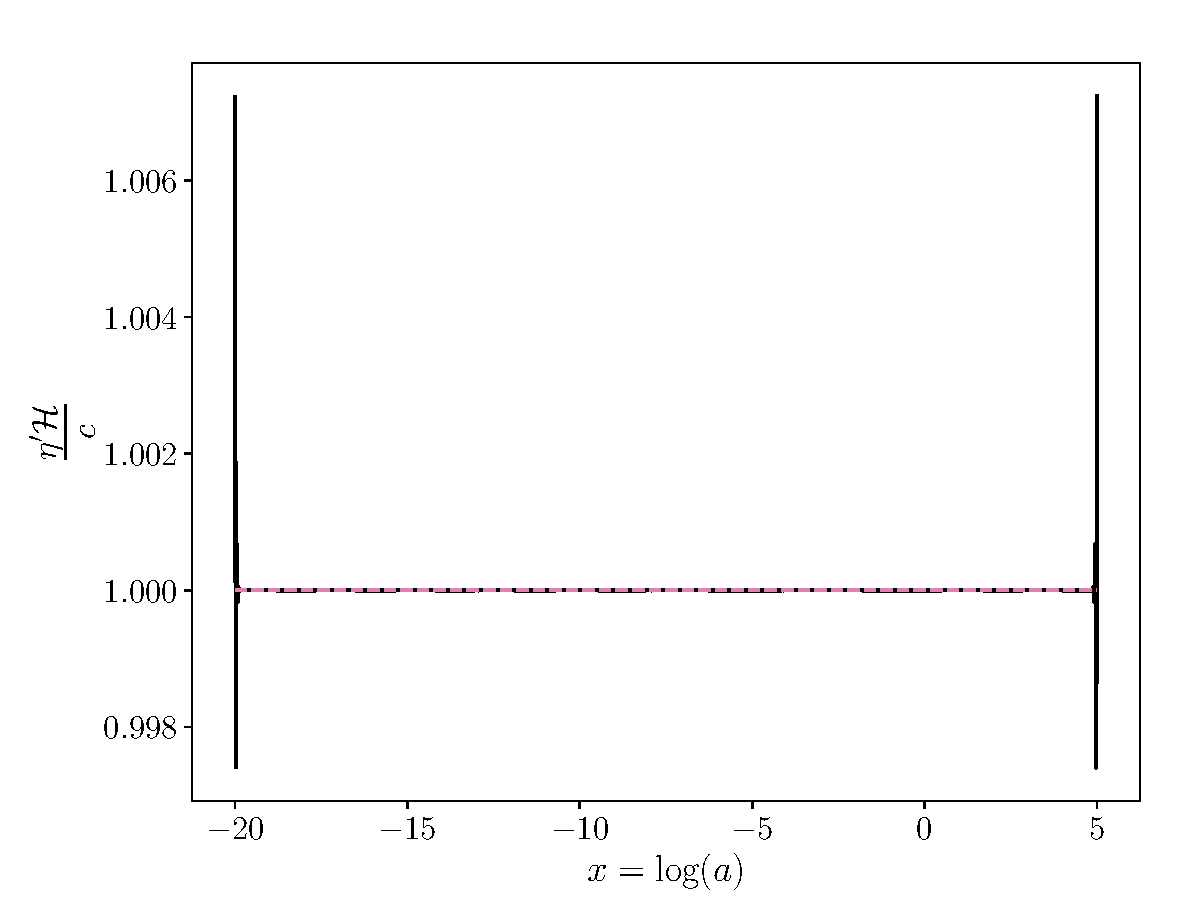
\includegraphics[width=\columnwidth]{/Users/paljettrosa/Documents/GitHub/AST5220/figs/numerical_stability.pdf}
    \caption{Comparison of the numerically computed conformal time derivative  $\eta'\mathcal{H}/c$ with the expected value of 1 (pink line). The small deviations on the order of $\lesssim 10^{-5}$ confirm the numerical stability of the integration.}\label{fig:numerical stability}
\end{figure}

To test the stability of the numerical solutions presented in the following section, I have plotted $\eta'\mathcal{H}/c$ as function of $x$ in figure \ref{fig:numerical stability}, since this quantity should remain close to unity throughout the range. The scatter points, which were obtained by taking the derivative of the spline for $\eta$, show small deviations from 1, on the order of $\lesssim 10^{-5}$, indicating that the numerical error is very small. It also remains bounded throughout the range of $x$, suggesting that the ODE solver maintains stability and does not accumulate significant numerical drift. The slight periodic variations could result from finite step sizes in the integration, or have something to do with interpolation errors between the integration points, but they are well within an acceptable tolerance.

As an additional test of the code, I ran it using a set of toy cosmological parameters chosen to match those used by \cite{Course}. The parameters are $h = 0.7$, $\Omega_\text{CDM0} = 0.45$, $\Omega_{b0} = 0.05$, $\Omega_{k0} = 0$, $N_\text{eff} = 0$ (implying $\Omega_{\nu0} = 0$), and $T_\text{CMB0} = 0.27255,\text{K}$, as in the fiducial model. The resulting plots, shown in figures \ref{appfig: Hp_and_eta}, \ref{appfig: eta_Hp_over_c}, and \ref{appfig: Omega_i} in appendix \ref{appsec: figures}, are visually indistinguishable from those published by Winther. This provides strong validation for the accuracy and reliability of the implementation.

\colorbox{Plum}{TODO: maybe move over prev. sec.}


\subsection{Results and discussions}\label{subsec: I results}

\subsubsection{The conformal Hubble parameter}
\begin{figure}
  \centering
  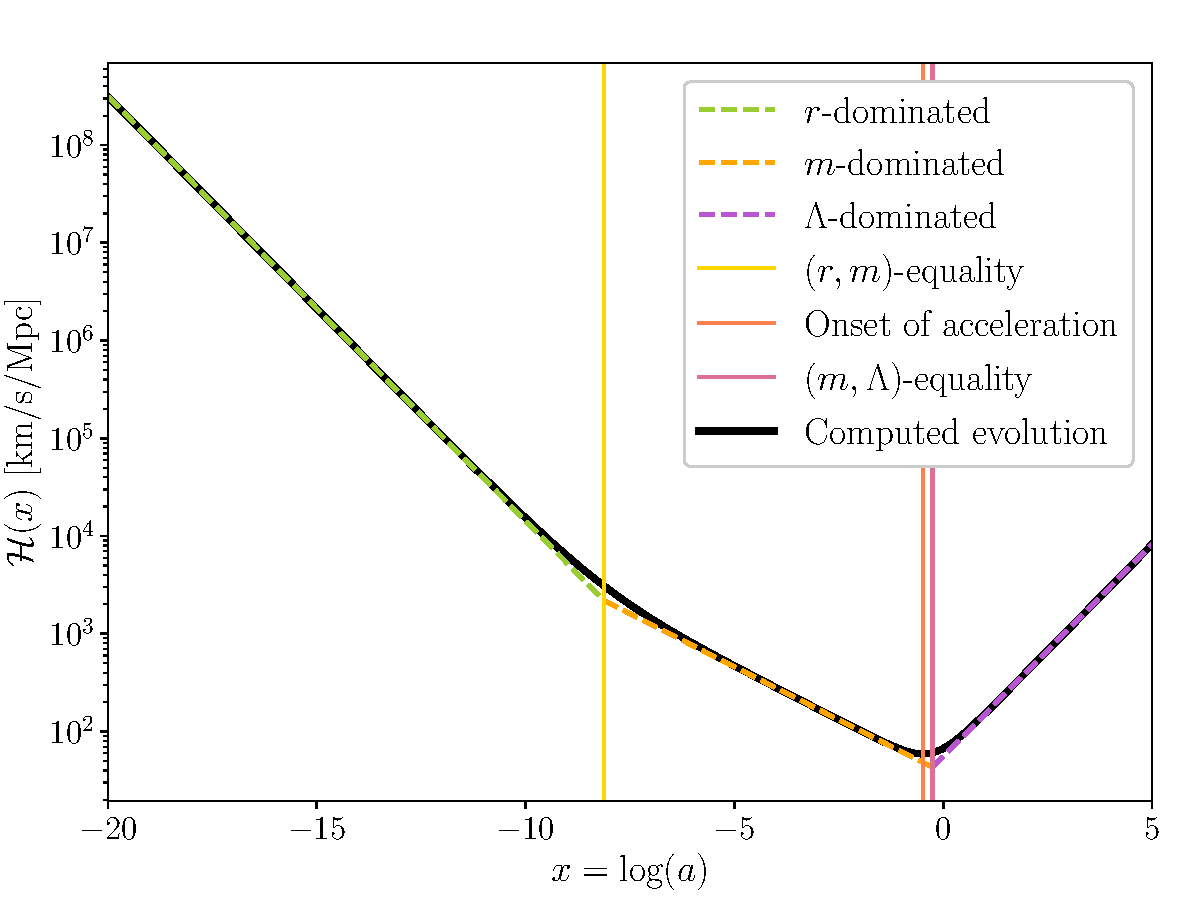
\includegraphics[width=\columnwidth]{/Users/paljettrosa/Documents/GitHub/AST5220/figs/H_prime.pdf}
  \caption{Exact evolution of the conformal Hubble parameter $\mathcal{H}(x)$ (black) compared with approximations (dashed). The onset of acceleration is visible as a departure from matter-like scaling, occuring at the trough of the exact solution.}\label{fig:H_prime}
\end{figure}


In figure \ref{fig:H_prime} I have plotted the exact evolution of the conformal Hubble parameter $\mathcal{H}(x)$ (black solid line), with approximations in the different cosmological epochs overplotted (dashed lines). Green, orange and purple correspond to radiation-, matter- and dark energy-dominated eras, respectively, with the yellow, red and pink vertical lines marking radiation-matter equality, onset of acceleration, and matter-dark energy equality. We see that the approximations closely follow the exact solution, staying at the correct order of magnitude at all times, although the deviations are significant close to the equality times. These are of course to be expected, since the approximations were derived under the assumption of the Universe only containing the dominating component within the different eras, which of course is not realistic as we transition from one to another. Thus, the result is still a great validation for the approximations, which indicates that we can safely use them to verify the numerical solutions for $\eta$ and $t$.

\begin{figure*}
    \centering
    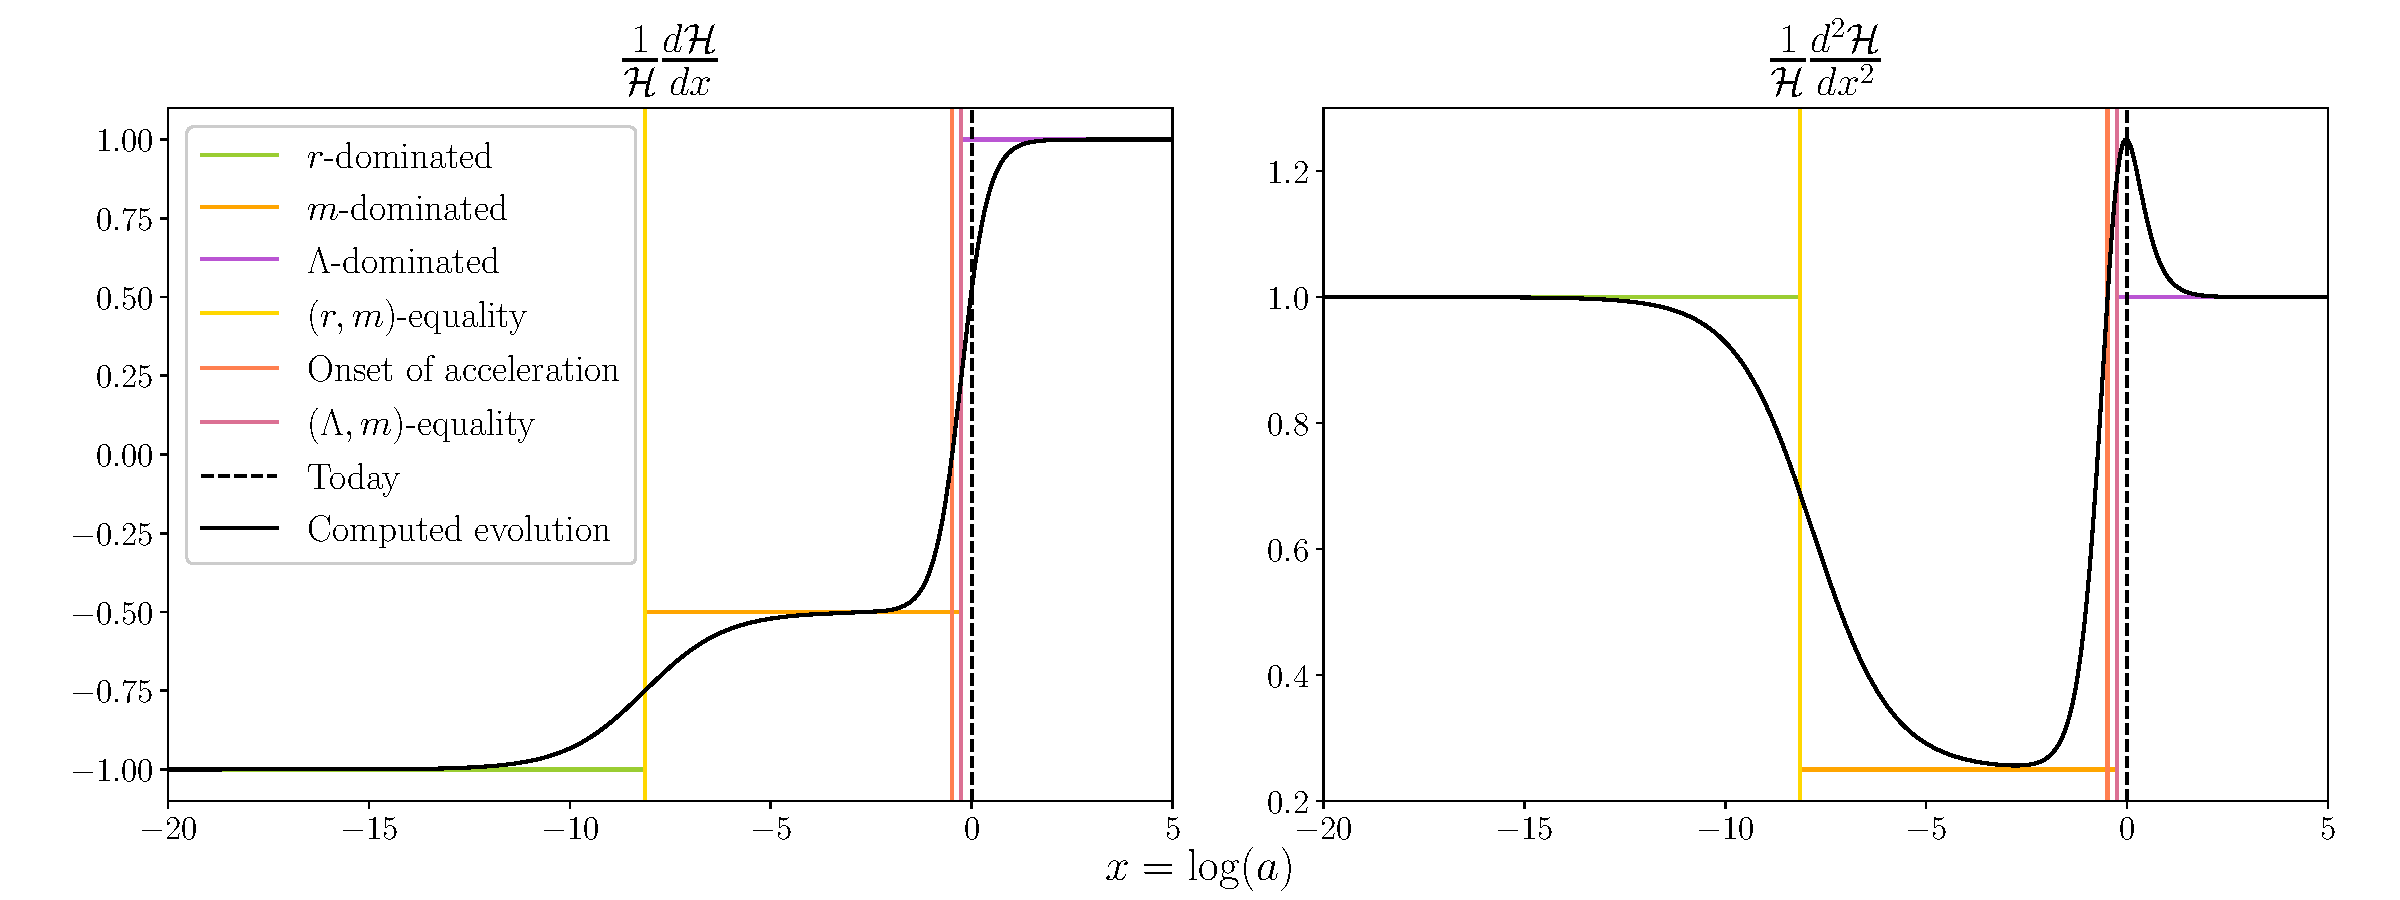
\includegraphics[width=\textwidth]{/Users/paljettrosa/Documents/GitHub/AST5220/figs/H_prime_derivatives.pdf}
    \caption{Comparison of exact evolutions (black) with approximations (dashed) for the scaled first and second derivatives of $\mathcal{H}(x)$. Agreement is good in pure radiation and matter domination but deviates near transitions due to neglected components.}\label{fig:H_prime derivatives}
\end{figure*}

A more direct comparison between the approximations and the exact evolution can be seen in figure \ref{fig:H_prime derivatives}, where I have plotted the first (left) and second (right) derivatives of $\mathcal{H}$ with respect to $x$, divided by $\mathcal{H}$ to see relative differences more easily. The dashed lines of different colors represent the same things here as well. We see good agreement in the asymptotically radiation-dominated and dark energy-dominated regimes, while in the matter-dominated epoch and around the equality times there are clear deviations, especially for the double derivative. This is reasonable, as we make rough approximations in both the beginning and the end of this era, hence the exact solution barely has time to sink to the expected value before it rises at the next transition point. 

It is interesting to see that the scaled double derivative actually increases beyond the expected value in the beginning of the dark energy-dominated era, with the peak being today. To understand this, we can look back at eqs. \eqref{eq:dHpdx} and \eqref{eq:ddHpddx}. The latter shows that the second derivative is influenced by a competition between growing and decaying terms as the Universe evolves: During the matter-dominated era, the dominant term is $\Omega_{m0} e^{-x}$, which leads to a slow decrease in $\mathcal{H}$; as $\Lambda$ begins to dominate, the exponential growth of the $2\Omega_{\Lambda 0} e^{2x}$ term starts accelerating the Universe. The transition is not instantaneous, meaning there is a period where the competing effects of matter dilution ($e^{-x}$) and dark energy growth ($e^{2x}$) cause a rapid shift in dynamics. This is visible in the sharp turn of $\mathcal{H}$ in figure \ref{fig:H_prime}, and explains the peak in the scaled second derivative before it settles into the $\Lambda$-dominated regime.


\subsubsection{Time and horizon measures}
\begin{figure*}
  \centering
  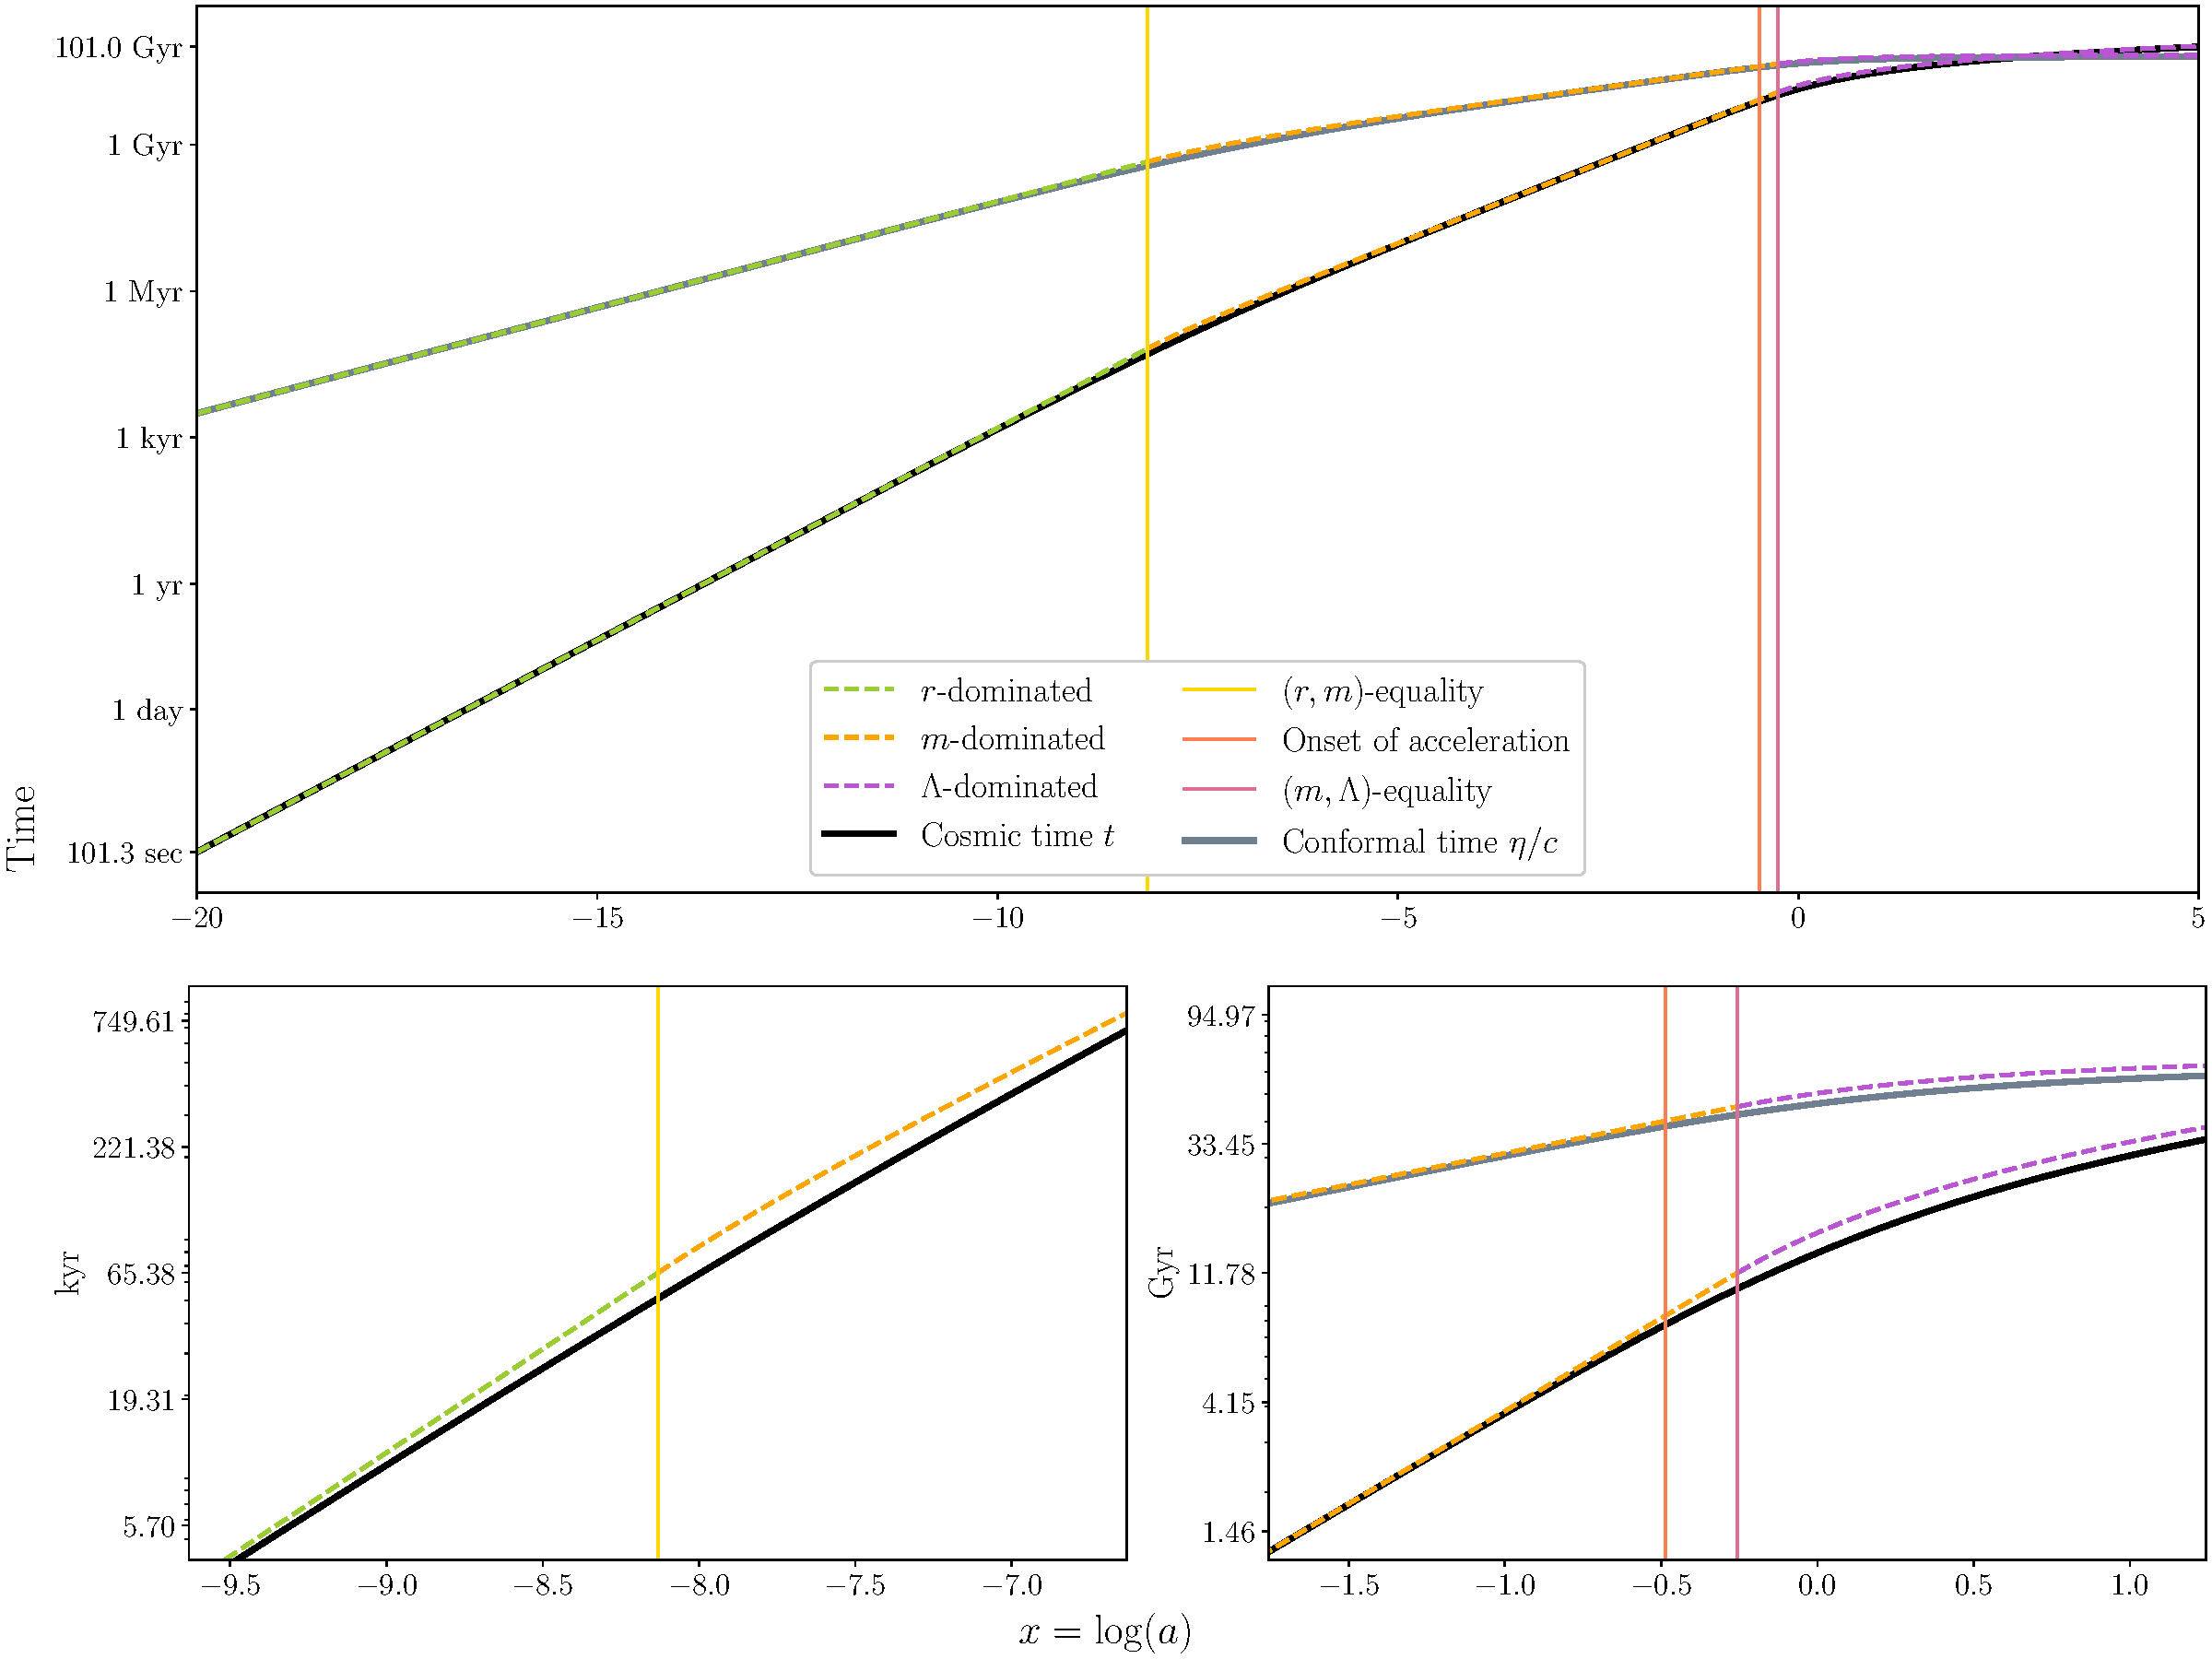
\includegraphics[width=\textwidth]{/Users/paljettrosa/Documents/GitHub/AST5220/figs/eta_and_t.pdf}
  \caption{Conformal time $\eta(x)$ (grey) and cosmic time $t(x)$ (black) compared with analytical approximations (dashed). Deviations near equality points arise due to gradual transitions between dominant energy components. This is highlighted in the bottom subplots for the cosmic time.}\label{fig:eta and t}
\end{figure*}

In figure \ref{fig:eta and t} I have plotted the numerical solutions for the conformal time $\eta/c$ (grey) and the cosmic time $t$ (black) as functions of $x$, with the approximate analytical solutions presented in section \ref{subsec: I theory} overplotted with dashed lines. The two bottom subplots, where the cosmic time is in focus, are included to easily be able to study what happens where the discrepancies between the numerical and analytical solutions are most drastic: where the Universe transitions from being dominated by one component to another. As expected, we see that the analytical approximation starts to deviate from the numerical curve as we approach $(r,m)$-equality, and eventually meets it again after. This happens also for the $(m,\Lambda)$-equality, but here the deviation actually continues to grow before it falls down again.


\begin{table*}
  \caption{Key cosmological timestamps at radiation-matter equality, the onset of acceleration, matter-dark energy equality, and present-day values. The analytical values are obtained using approximations from the theory section, while the numerical values are extracted from splines after solving the full system of equations. Discrepancies between the two highlight the limitations of the analytical approximations, especially during transition epochs.}             % title of Table
  \label{table:time stamps}      % is used to refer this table in the text
  \centering                          % used for centering table
  \begin{tabular}{| c || c | c | c | c |}        % centered columns (4 columns)
  \hline                % inserts double horizontal lines
   & Radiation-matter equality & Onset of acceleration & Matter-dark energy equality & Present day values \\    % table heading 
  \hline\hline                        % inserts single horizontal line
  \hspace{6pt}$x$\hspace{53pt} & \hspace{8.5pt}$-8.13$ & $-0.49$ & $-0.26$ & 0 \\      % inserting body of the table
  \hline 
  \hspace{6pt}$z$\hspace{53pt} & $3400.33$ & \hspace{6.5pt}$0.63$ & \hspace{7pt}$0.29$  & 0 \\
  \hline 
  \hspace{6pt}$t$ \hspace{5pt}(analytical) & \hspace{25pt}$65.38\,$kyr & \hspace{24.5pt}$8.33\,$Gyr & \hspace{19pt}$11.78\,$Gyr & \hspace{25pt}$16.30\,$Gyr \\
  \hspace{6pt}$t$ \hspace{5pt}(numerical) & \hspace{25pt}$51.06\,$kyr & \hspace{24.5pt}$7.75\,$Gyr & \hspace{19pt}$10.38\,$Gyr & \hspace{25pt}$13.86\,$Gyr \\
  \hline 
     $\eta/c$ (analytical) & \hspace{25pt}$444.75\,$Myr & \hspace{20.5pt}$40.22\,$Gyr & \hspace{19pt}$45.20\,$Gyr & \hspace{25pt}$50.36\,$Gyr \\ 
     $\eta/c$ (numerical) & \hspace{25pt}$368.44\,$Myr & \hspace{20.5pt}$38.57\,$Gyr & \hspace{19pt}$42.37\,$Gyr & \hspace{25pt}$46.32\,$Gyr \\ 
     \hline 
     \hspace{5.5pt}$\eta$ \hspace{3.5pt}(analytical) & \hspace{25pt}$136.27\,$Mpc & \hspace{20.5pt}$12.32\,$Gpc & \hspace{19pt}$13.85\,$Gpc & \hspace{25pt}$15.43\,$Gpc \\ 
     \hspace{5.5pt}$\eta$ \hspace{3.5pt}(numerical) & \hspace{25pt}$112.89\,$Mpc & \hspace{20.5pt}$11.82\,$Gpc & \hspace{19pt}$12.98\,$Gpc & \hspace{25pt}$14.19\,$Gpc \\ 
  \hline                                   %inserts single line
  \end{tabular}
  \end{table*}

In table \ref{table:time stamps} I have listed key cosmological timestamps for important transition points in the Universe's history: radiation-matter equality, the onset of acceleration, matter-dark energy equality, and present-day values. The logarithmic scale factor $x = \log (a)$ and redshift $z$ are listed for each event, along with analytical and numerical results for cosmic time $t$, conformal time $\eta/c$, and the comoving horizon $\eta$. We observe a discrepancy between the analytically approximated values for $t$ and $\eta$ obtained using the expressions derived in section \ref{subsec: I theory} and the corresponding numerical values, which instead were obtained by solving the full system of equations and interpolating via splines. These discrepancies are consistent with figure \ref{fig:eta and t}. \colorbox{Plum}{compare r-m eq w/ Planck!}

In \citet{Planck}, one presented estimate of the age of the Universe is $t_0=13.801\pm0.024\,\text{Gyr}$. This is based on $1\sigma$ constraints on a combination of gravitational lensing and TT (temperature), TE (temperature-E mode polarization), EE (E mode polarization) and lowE (low multipole E-mode polarization) angular power spectra measurements. This is in good agreement with the numerical result, although the value stated here is slightly larger. Nevertheless, the analytical approximation greatly overestimate it in comparison. This further validates the numerical solution around the equality times, where it deviates from the approximate evolutions and we have less to compare it to.

\subsubsection{Density parameters}
\begin{figure}
    \centering
    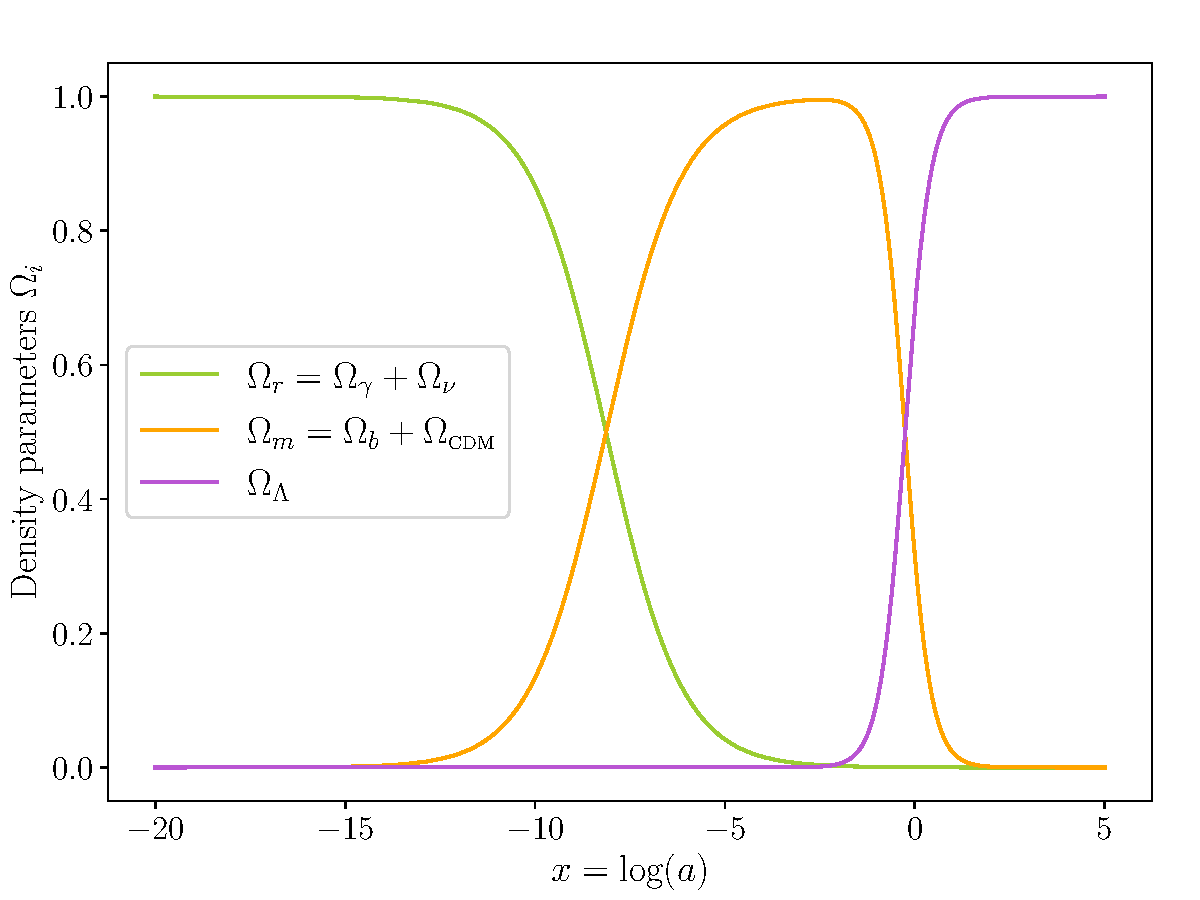
\includegraphics[width=\columnwidth]{/Users/paljettrosa/Documents/GitHub/AST5220/figs/density_parameters.pdf}
    \caption{The fractional energy densities of radiation, matter, and dark energy as functions of $x$ (solid lines). The dashed lines show the evolutions of the radiation components (photons and neutrinos) and matter components (baryons and dark matter).}\label{fig:density parameters}
\end{figure}

The evolutions of the density parameters $\Omega_i(x)$ are plotted in figure \ref{fig:density parameters}, with solid lines for $\Omega_r$, $\Omega_m$ and $\Omega_\Lambda$, and dashed lines for the individual components that make up the two first of these. The solid curves are consistent with the previous results, with the transitions between the different eras matching the observed changes in $\mathcal{H}$, $\eta$ and $t$. For example, the abrupt change in the conformal Hubble parameter at $(m,\Lambda)$-equality compared to the change at $(r,m)$-equality matches the relatively rapid takeover of $\Lambda$ as the dominating energy component, as opposed to the more gradual change from radiation to matter domination. 

\subsubsection{Supernova fitting}
% \begin{table}
%   \caption{Best-fit cosmological parameters obtained from supernova data, along with their mean values and standard deviations. The best-fit values correspond to the minimum $\chi^2$, while the Planck 2018 values are provided for comparison. The Hubble constant $H_0$ is given in units of km/s/Mpc.}             % title of Table
%   \label{table:supernova}      % is used to refer this table in the text
%   \centering                          % used for centering table
%   \begin{tabular}{| c || c | c | c | c |}        % centered columns (4 columns)
%   \hline                % inserts double horizontal lines
%    & \hspace{5pt}$\mu_i$\hspace{5pt} & \hspace{7pt}$\sigma_i$\hspace{7pt} & min$\big(\chi^2\big)$ & Planck \\    % table heading 
%   \hline\hline                     % inserts single horizontal line
%   $H_0$ & \hspace{-10pt}70.1 & \hspace{-10pt}0.5 & \hspace{-10pt}70.2 & \hspace{-10pt}67.0 \\
%   \hline
%   $\Omega_{m0}$ & \hspace{5pt}0.240 & 0.087 & \hspace{5pt}0.258 & \hspace{5pt}0.317 \\
%   \hline
%   $\Omega_{k0}$ & \hspace{5pt}0.118 & 0.216 & \hspace{5pt}0.071 & \hspace{5pt}0.000 \\
%   \hline
%   $\Omega_{\Lambda0}$ & \hspace{5pt}0.642 & 0.133 & \hspace{5pt}0.672 & \hspace{5pt}0.683 \\
%   \hline                                   %inserts single line
%   \end{tabular}
% \end{table}

\begin{table}
  \caption{Best-fit cosmological parameters obtained from supernova data, along with their mean values and standard deviations. The best-fit values correspond to the minimum $\chi^2$, while the Planck 2018 values estimated from 1$\sigma$ constraints on TT,TE,EE+lowE+lensing measurements are provided for comparison. These were determined by assuming a perfectly flat Universe, though they do actually estimate a small non-zero curvature density ($\Omega_{k0}=0.0007\pm0.0019$) when relaxing this assumption and also including BAO measurements. I have chosen to neglect this in my analysis, due to the relatively small value and large uncertainty. \colorbox{Plum}{move to main text?} Moreover, the Hubble constant is given in units of km/s/Mpc.}             % title of Table
  \label{table:supernova}      % is used to refer this table in the text
  \centering                          % used for centering table
  \begin{tabular}{| c || c | c | c | c |}        % centered columns (4 columns)
  \hline                % inserts double horizontal lines
   & \hspace{5pt}$\mu_i$\hspace{5pt} & \hspace{7pt}$\sigma_i$\hspace{7pt} & min$\big(\chi^2\big)$ & Planck \\    % table heading 
  \hline\hline                     % inserts single horizontal line
  $H_0$ & \hspace{-10pt}70.1 & \hspace{-10.2pt}0.5 & \hspace{-10.8pt}70.2 & \hspace{-5.5pt}$67.4\pm0.5$ \\
  \hline
  $\Omega_{m0}$ & \hspace{4.8pt}0.240 & \hspace{-0.2pt}0.087 & \hspace{4.6pt}0.258 & $0.315\pm0.007$ \\
  \hline
  $\Omega_{k0}$ & \hspace{0pt}0.12 & \hspace{-5pt}0.22 & \hspace{0pt}0.07 & 0 \\
  \hline
  $\Omega_{\Lambda0}$ & \hspace{5pt}0.642 & 0.133 & \hspace{5pt}0.672 & $0.685\pm0.007$ \\
  \hline                                   %inserts single line
  \end{tabular}
\end{table}


When running the MCMC fits, the minimum chi-squared value obtained was $\chi^2_\text{min}=29.2867$, corresponding to the parameter values listed in the third column of table \ref{table:supernova}. The means $\mu_i$ and standard deviations $\sigma_i$ (where $i$ runs over the parameters) computed for the samples within the $1\sigma$ constraints are listed as well, in addition to the Planck parameters stated in \cite{Planck} for comparison. Interestingly, the supernova measurements favor a slightly open universe, deviating from the Planck result of a flat universe. However, the standard deviation, which is about three times larger than the best-fit value, suggests that the data does not strongly constrain curvature. We also see that the Planck result for $\Omega_{m0}$ is higher than the best-fit value, though it is within the $1\sigma_m$ confidence interval. 
% Nevertheless, this suggests that the supernova data prefers a lower matter density, which is consistent with the higher inferred value of $H_0$. 
% Lastly, the Planck value for $\Omega_{\Lambda0}$ is only slightly larger than the best-fit value, and it is well within $1\sigma_\Lambda$. \colorbox{Plum}{correct to say this?}.

\begin{figure}
    \centering
    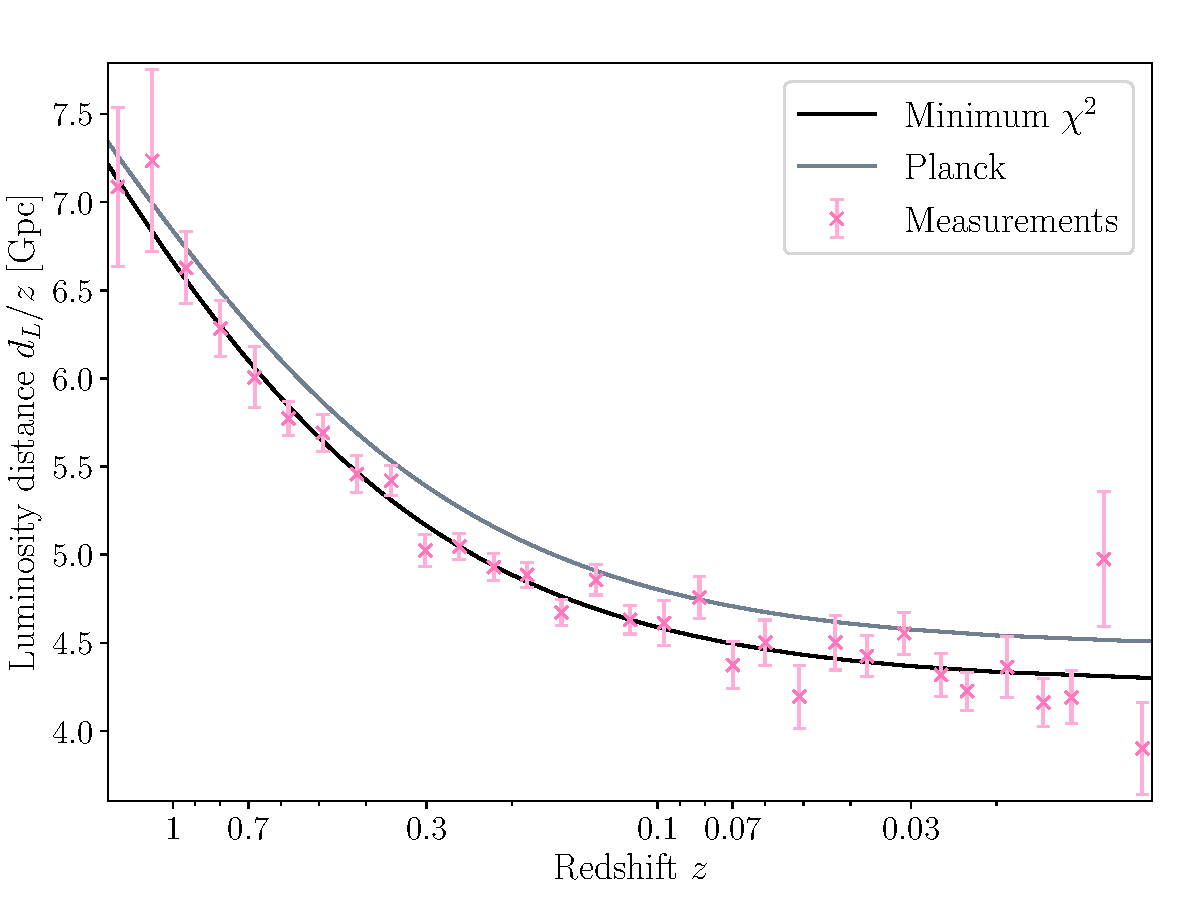
\includegraphics[width=\columnwidth]{/Users/paljettrosa/Documents/GitHub/AST5220/figs/luminosity_distance.pdf}
    \caption{Comparison of the luminosity distances $d_L^\text{obs}/z$ gathered from supernova observations (pink with errorbars) with the fiducial Planck model (grey) and the best-fit model from MCMC analysis (black).}\label{fig:luminosity distance}
\end{figure}

After obtaining the best-fit values I made a new instance of \verb|BackgroundCosmology| with these parameters and solved for this universe as well. In figure \ref{fig:luminosity distance} I have plotted the scaled luminosity distance $d_L/z$ against $z$ for this best-fit cosmology (black curve) as well as the Planck cosmology (grey curve), together with the data points $d_L^\text{obs}/z$ with scaled errorbars (pink). We see that the best-fit cosmology aligns much better with the data points than the Planck model, as the latter does not always lie within the supernova errorbars. This reflects the fact that the Planck data prefers a flat universe, whereas the best-fit suggests slightly negative curvature, which alters the distance-redshift relation. It also highlights tensions between low-redshift and high-redshift cosmological probes (see e.g. \cite{JWST} for a recent discussion of this so-called Hubble tension in light of JWST observations). However, it should be kept in mind that measurements of supernova magnitudes can be affected by calibration uncertainties, host galaxy effects and dust extinction, potentially shifting best-fit cosmological parameters. Nevertheless, the discrepancies underscore the importance of using multiple probes and datasets to break parameter degeneracies and obtain a more complete picture of cosmic expansion.


\begin{figure}
    \centering
    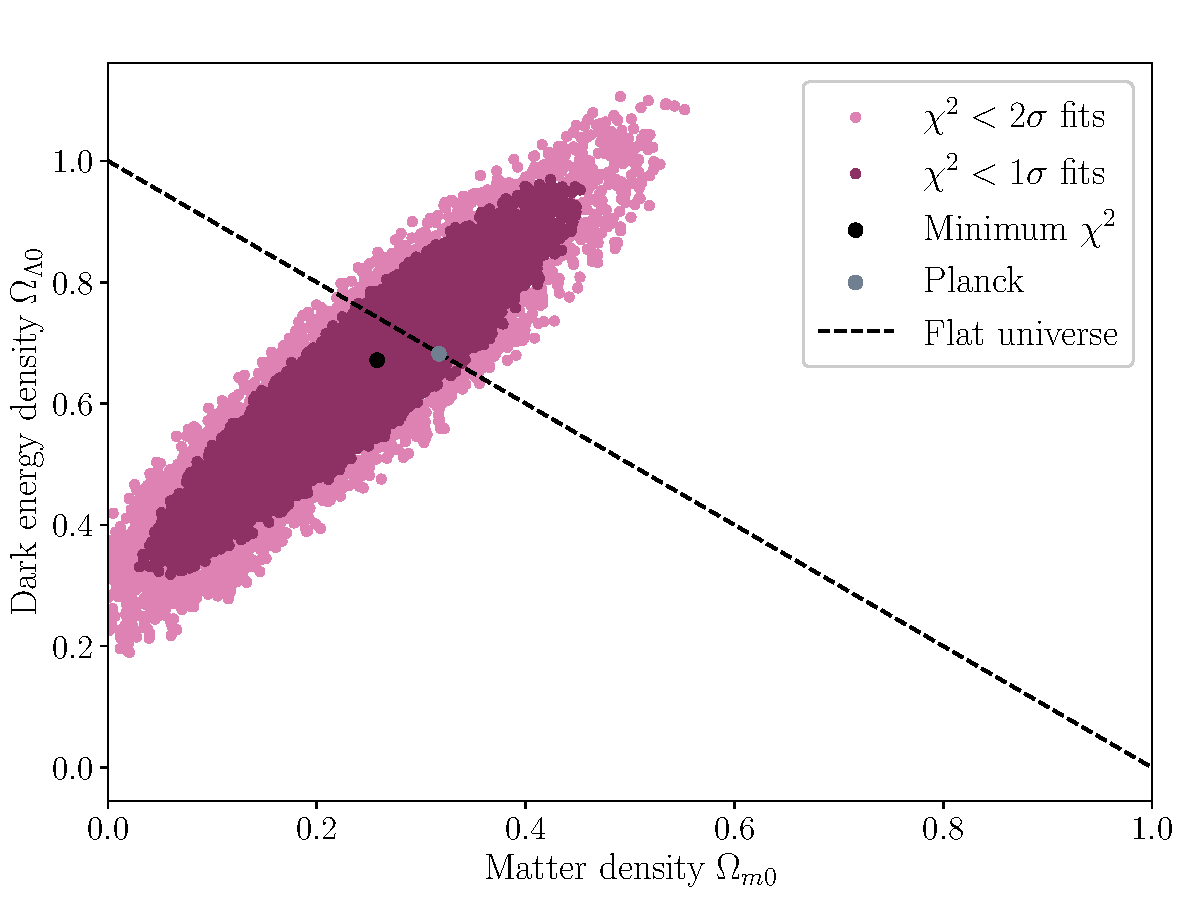
\includegraphics[width=\columnwidth]{/Users/paljettrosa/Documents/GitHub/AST5220/figs/MCMC_fits.pdf}
    \caption{Confidence contours in the $(\Omega_{m0},\Omega_{\Lambda0})$ parameter space from the supernova MCMC analysis, compared to the Planck fiducial model. The supernova constraints allow for a slightly open universe, while Planck favors flatness based on multi-probe data.}\label{fig:MCMC fits}
\end{figure}

In figure \ref{fig:MCMC fits} I have scatter plotted the accepted $(\Omega_{m0},\Omega_{\Lambda0})$ samples within the $1\sigma$ and $2\sigma$ constraints, with the black (grey) data point showing the best-fit (Planck) parameter set, and the dashed line showing the combinations that allow for a flat universe. We see clearly here that supernova-only constraints allow for slightly different cosmologies than the Planck model, with a preference for a lower matter density and small negative curvature. The Planck data includes additional information from the early universe, leading to a tighter preference for a flat universe with more mass. This discrepancy ties directly to the luminosity distance plot, confirming that these best-fit supernova parameters slightly differ from Planck's and further highlighting the importance of combining multiple datasets for robust cosmological constraints.


% When running the MCMC fits, the minimum chi-squared value obtained was $\chi^2_\text{min}=29.2867$, corresponding to the parameter values listed in the third column of table \ref{table:supernova}. The means $\mu_i$ and standard deviations $\sigma_i$ (where $i$ runs over the parameters) computed for the samples within the $1\sigma$ constraints are listed as well, in addition to the Planck parameters for comparison. We see that the best-fit value of $H_0$ based on the supernova data alone was $70.204\,$km/s/Mpc, slightly higher than the Planck result of $67\,$km/s/Mpc. This is expected, as supernova data alone tends to favor a higher $H_0$ than CMB-based analyses, a discrepancy known as the Hubble tension. We also see that the Planck result is larger than the best-fit value for $\Omega_{m0}$, though it is within $1\sigma_m$ \colorbox{Plum}{correct to say this?}. Nevertheless, this suggests that the supernova data prefers a lower matter density, which is consistent with the higher inferred value of $H_0$.

% Interestingly, the results favor a slightly open universe, deviating from the Planck result of a flat universe. However, the standard deviation, which is about three times larger than the best-fit value, suggests that the data does not strongly constrain curvature. Lastly, the Planck value for $\Omega_{\Lambda0}$ is only slightly larger than the best-fit value, and it is well within $1\sigma_\Lambda$. \colorbox{Plum}{correct to say this?}. These results highlight the differences between constraints obtained from supernova data alone versus those obtained from CMB measurements. The larger uncertainties in our fits, particularly for $\Omega_{k0}$, emphasize the need to incorporate additional cosmological probes, such as baryon acoustic oscillations (BAO) and CMB data, for tighter constraints.

\begin{figure*}
  \centering
  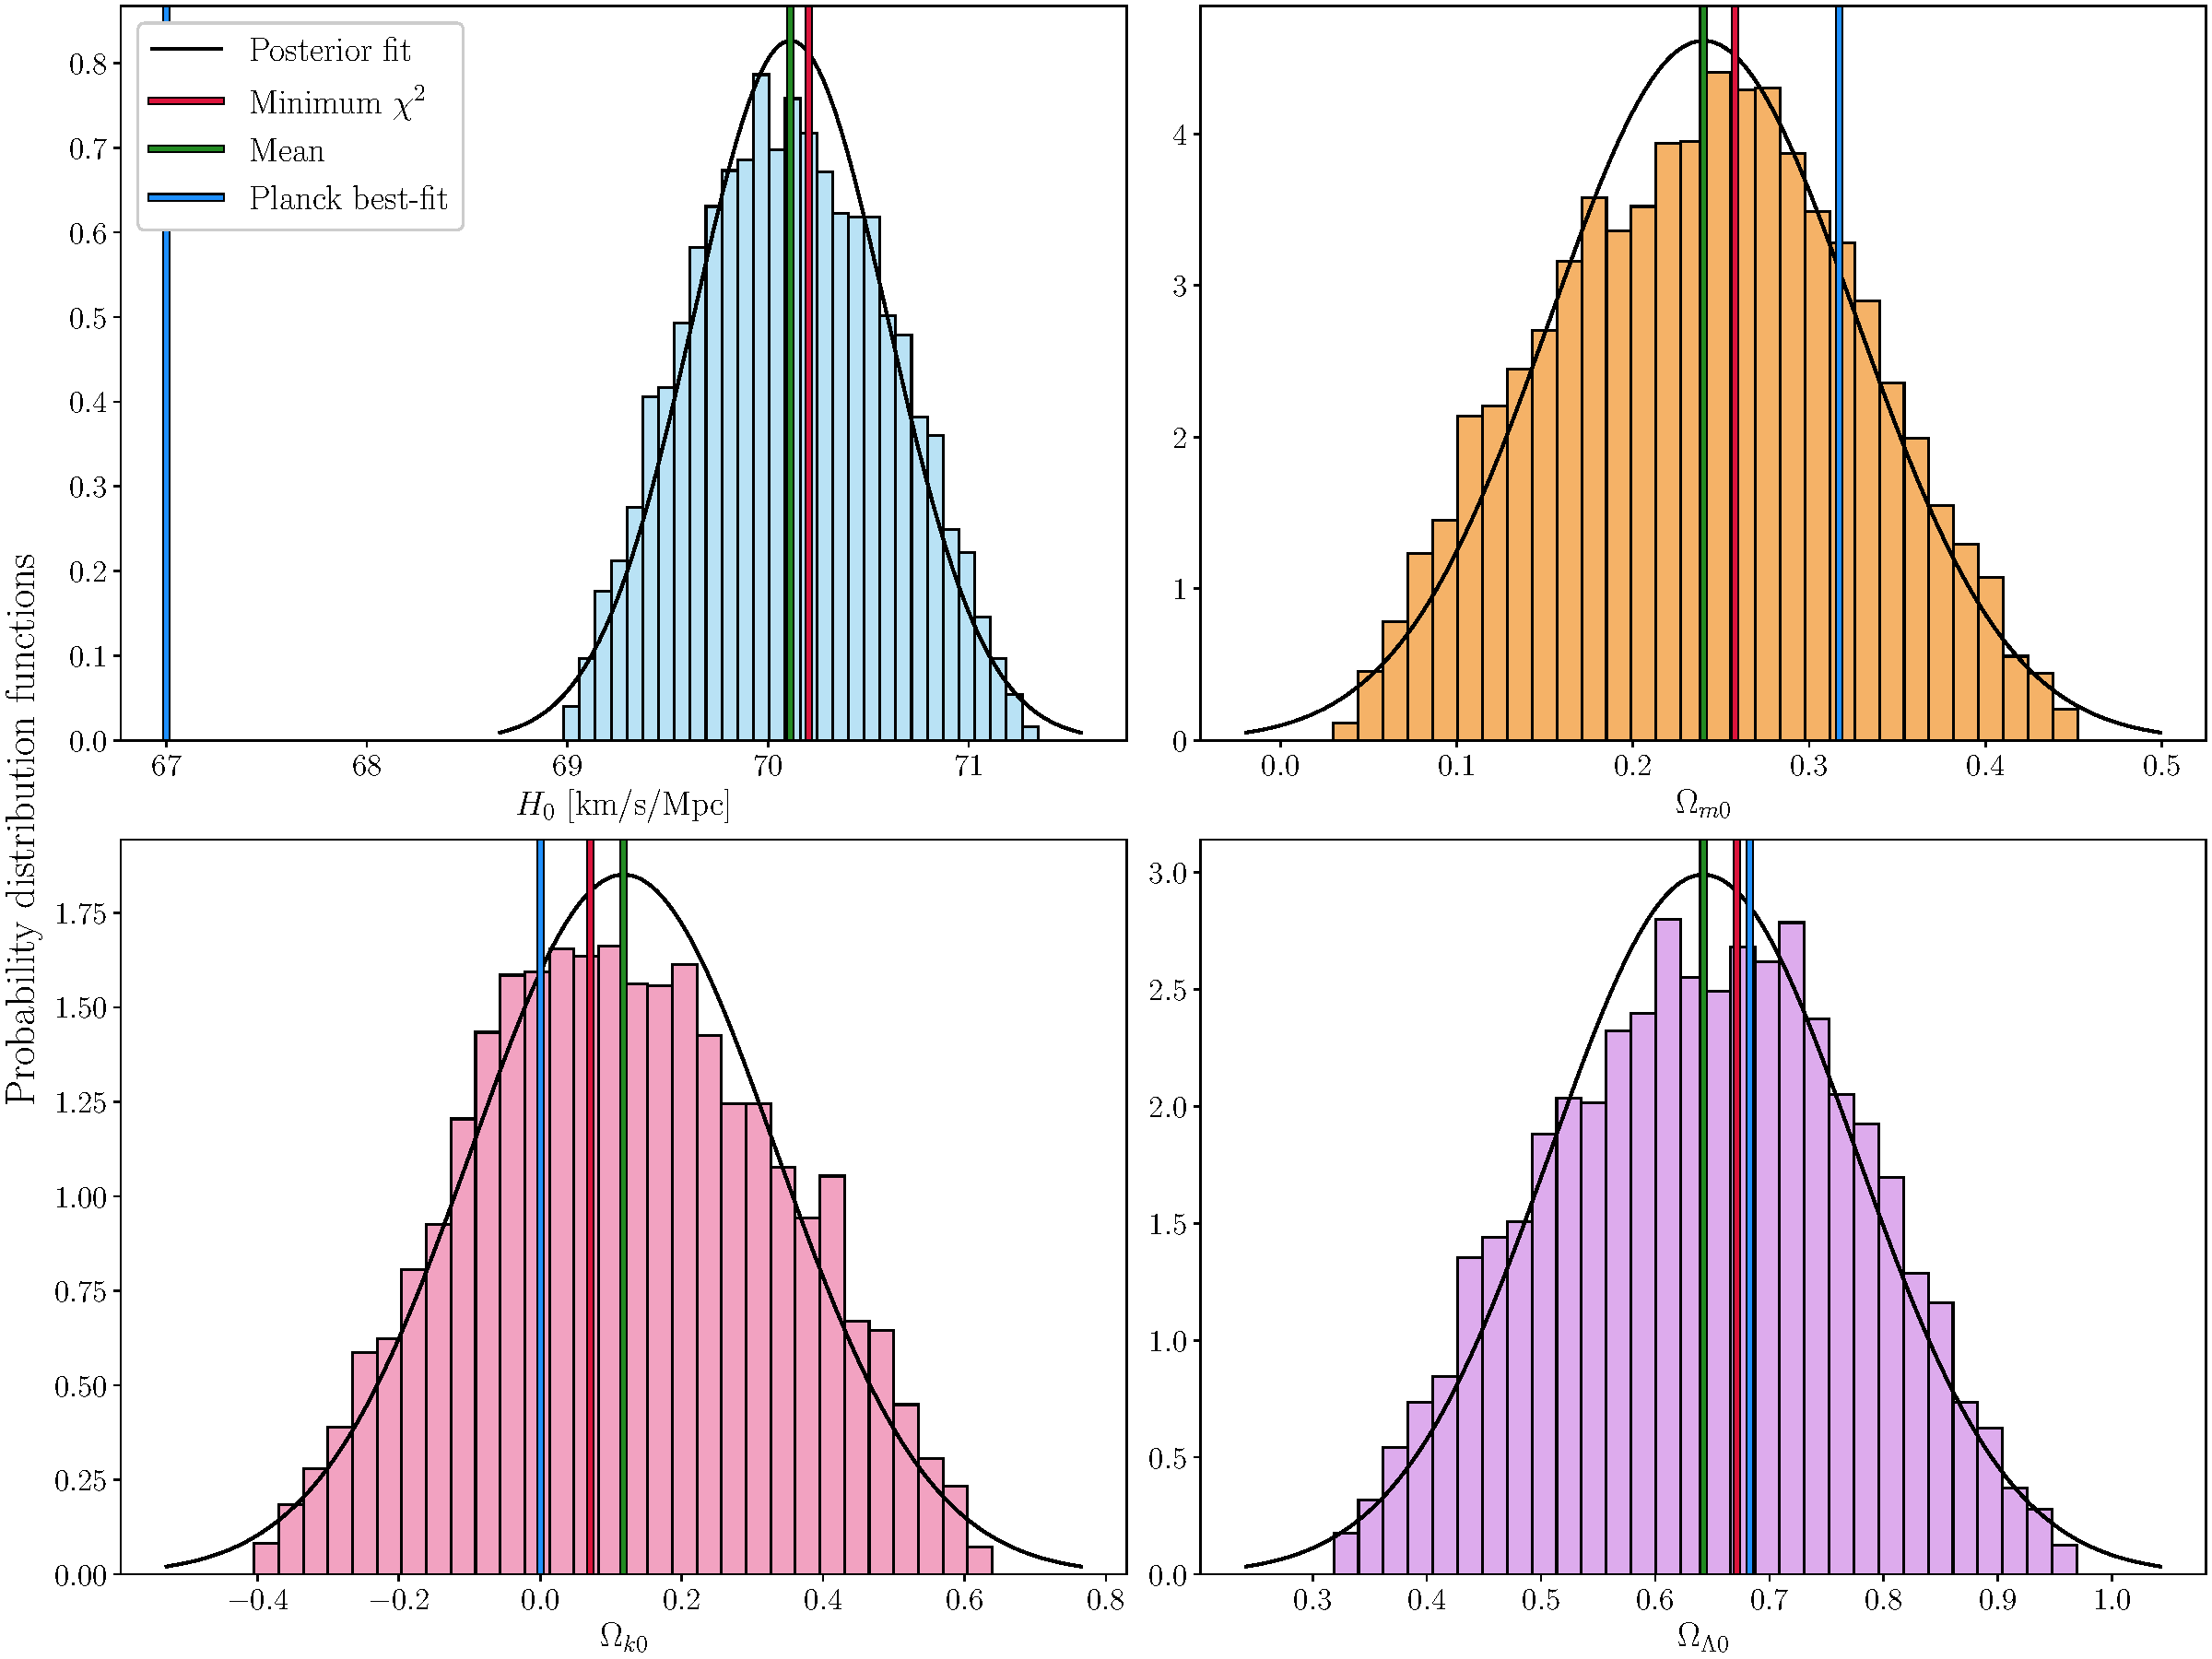
\includegraphics[width=\textwidth]{/Users/paljettrosa/Documents/GitHub/AST5220/figs/distributions.pdf}
  \caption{Histograms of the MCMC posterior distributions for the parameters $(H_0,\Omega_{m0}, \Omega_{k0}, \Omega_{\Lambda0})$, compared with Gaussian fits (solid curves) and Planck values. Deviations from Gaussianity indicate asymmetries in parameter uncertainties.}\label{fig:distributions}
\end{figure*}

Figure \ref{fig:distributions} shows normalized histograms of the samples within the 1$\sigma$ constraint, with Gaussian fits made with the $\mu_i$ and $\sigma_i$ overplotted to represent the posterior distributions. Most noticeable is how different the supernova and Planck results are for $H_0$, with the smallest accepted $1\sigma$ samples being as large as $69\,$km/s/Mpc. Planck's estimate is derived from early universe physics (CMB, baryon acoustic oscillations and large-scale structure), while supernova constraints come from low-redshift expansion. The discrepancy may therefore indicate new and/or unknown physics present at some eras of the expansion history (see \cite{JWST}, but also \cite{tensions} for critical discussions on tensions as indicators of new physics), or possibly systematic errors in one or both datasets. Moreover, we see that the supernova-only constraint clearly prefers a lower matter density compared than the Planck estimate, consistent with the MCMC contour plot.

The posterior distribution suggests a preference for a slightly open universe, though with considerable uncertainty. This deviation from flatness may arise because supernovae alone do not tightly constrain curvature, as they primarily measure relative distances, not absolute spatial curvature. Moreover, we see that the histograms are not perfectly Gaussian, particularly those for $\Omega_{m0}$ and $\Omega_{k0}$. Specifically, the asymmetry with more samples in the low mass/negative curvature ends may suggest a skewed uncertainty, indicating that a simple Gaussian error estimate might underestimate the possible range of accepted values. 

\colorbox{Plum}{maybe remove/argue for good in ast. standards}
% Alarmingly, the $H_0$ distribution appears more symmetric, indicating that supernova data alone provide a more stable estimate for the Hubble constant, which deviates the most from the Planck result.




\section{Milestone II: Recombination History}\label{sec: milestone II}
I got feedback on this paragraph from the milestone II intro, saying it was good but that initial conditions was not a good word to use in the last sentence. Can you suggest an alternative?

In the previous milestone, I established a numerical framework for solving the background evolution of the Universe, validating the results against analytical approximations and observational constraints. This provided a foundation for understanding the expansion history and cosmic distances, key ingredients in interpreting cosmological data. However, to model the formation of the CMB and its anisotropies, we must now extend the analysis to include recombination history: the period when the Universe transitioned from an ionized plasma to a neutral state, allowing photons to decouple from matter. This process determines the surface of last scattering, setting the conditions at decoupling that shape the CMB fluctuations we observe today.  

In this milestone, I compute the recombination and reionization history by solving the Saha and Peebles equations, track the evolution of the optical depth $\tau(x)$, and derive the visibility function $\tilde{g}(x)$, which quantifies when CMB photons last interacted with free electrons. These quantities are essential for accurately modeling the temperature and polarization anisotropies of the CMB in the next milestones. Additionally, I compute the sound horizon at decoupling, a fundamental scale imprinted in the CMB power spectrum. This milestone bridges the gap between background cosmology and perturbation theory, ensuring that my model of the early Universe correctly captures the physics governing photon-matter interactions before recombination. 


\subsection{Theoretical framework}\label{subsec: II theory}
% \begin{enumerate}
%   \item [1.] Write out the distribution function $f$ for fermions and bosons, and show that it reduces to the Maxwell-Boltzmann distribution in the low energy limit.
%   \item [2.] State the Boltzmann equation in general relativity, written in terms of an affine parameter $\lambda$, the time $t$, the spatial components $x^i$, the energy $E$, the zero'th component of the four-momentum $P^0$, and the unit three-momentum vector $\hat{p}^i$. Explain that we use the unit vector since it vanishes in linear perturbation theory? Define also the moments of the Boltzmann equation (number density, energy density apnd pressure).
%   \item [3.] Explain what the collision term is, and that we will simply use results from quantum field theory calculations. Explain that it is zero in a smooth universe where the particles are in equilibrium with the thermal bath.
%   \item [4.] Explain that we usually consider $1+2\leftrightarrow3+4$ processes in cosmology, such as electron-positron annihilation and pair production, Compton (Thompson i low energy limit?) and Coulomb scattering, and hydrogen recombination / ionization. Write out these interaction processes. 
%   \item [5.] Explain which interaction is relevant at this point in time and for the CMB: Compton scattering in the low energy limit (Thompson scattering), and explain why this is the most important.
%   \item [6.] Write out the Boltzmann equation for such a process in a smooth universe, and explain what the parameters $\alpha$ and $\beta$ are. Explain that $\beta$ is defined in terms of $\alpha$ and the equilibrium number density values.
%   \item [7.] Explain what decoupling and freeze-out is, and define these limits in terms of the Boltzmann equation. Explain why it is crucial for our purposes.
%   \item [8.] Explain that it is hard to know exact number densities and that we instead use the fraction parameters. Define these and state all the fraction parameters (free electron fraction $X_e$, primordial Helium fraction $Y_p$, as well as $x_\text{He++}$, $x_\text{He+}$ and $x_\text{H+}$).
%   \item [9.] Derive the Saha approximation, and state the Saha equations when including Helium.
%   \item [10.] Move on to explain that we need the Peebles equation when the free electron fraction $X_e<0.99$, and state this. State also all of the atomic physics constants. Make sure to include Helium.
%   \item [11.] Explain how we can improve the results by including the fudge factor $f$ to the Peebles equation, and reference Recfast.
%   \item [12.] Define the optical depth, and explain that this is a crucial quantity that we need to have a firm grasp on. Derive its first and second derivatives with respect to $x$, and explain why we must integrate it in the same way as we did for $\eta$ and $t$, but starting from today's value.
%   \item [13.] Define the visibility function and explain its importance, and what it represents. Derive its first and second derivatives with respect to $x$.
%   \item [14.] Define the optical depth for baryons, and explain why it is important to include it for accuracy. Explain what the baryon drag epoch is.
%   \item [15.] Explain that a typical approximation to make is to set the baryon temperature equal to the photon temperature at all times, but that it is necessary to include it for full accuracy. Derive the baryon temperature equation from the Boltzmann equation, and compare it to the photon temperature equation.
%   \item [16.] Define the sound horizon, and explain why we need to know it at decoupling, and why it will be interesting to know it at the drag epoch.
%   \item [17.] Explain what reionization is, why it happened and why we should include it for accurate results. State the relevant equations, and explain that we must ``turn it off'' when computing certain quantities, such as the freeze-out abundance of free electrons today.
% \end{enumerate}

% Point 1 is for subsection 1, points 2-7 for subsection 2, point 8 for subsection 3, 9 for subsection 4, 10 and 11 for subsection 5, 12-14 for subsection 6, 15 for subsection 7, 16 for subsection 8, and point 17 for subsection 9. 

% Can you write subsection 8 about sound horizons? Make sure to include point 16. Be concise and thorough, and match my writing style from the previous milestone.



% \subsubsection{Distribution functions and the Boltzmann equation}
% \subsubsection{Distribution functions}
% In cosmology, the evolution of particle species is governed by their phase-space distribution function, $f$, which describes the number density of particles in a given region of phase space. For a system in thermal equilibrium, the distribution function is dictated by quantum statistics, specifically the Fermi-Dirac (+) and Bose-Einstein (-) distributions:
% \begin{equation}
% f(E) = \frac{1}{e^{(E - \mu) / T} \pm 1}.
% \end{equation}
% Here, $E$ is the energy of the particle, $\mu$ is the chemical potential, and $T$ is the temperature of the system. \colorbox{Plum}{match lecture notes?} The difference in the denominator arises due to quantum effects: bosons (minus sign in denominator) obey Bose-Einstein statistics and exhibit stimulated emission, while fermions (plus sign) obey the Pauli exclusion principle, preventing multiple particles from occupying the same state. \colorbox{Plum}{redundant?}

% Since the full distribution function is difficult to track, we instead take moments of the Boltzmann equation to extract physically relevant quantities. The number density $n$, energy density $\rho$, and pressure $P$ are given by weighted integrals over momentum space:
% \begin{align}
% n &= \frac{g}{(2\pi)^3} \int f d^3p, \\
% \rho &= \frac{g}{(2\pi)^3} \int E f d^3p, \\
% P &= \frac{g}{(2\pi)^3} \int \frac{p^2}{3E} f d^3p.
% \end{align}
% Here, $g$ represents the number of internal polarization states of the relevant particle species. Taking moments of the Boltzmann equation allows us to derive conservation equations, which describe how mass, momentum, and energy evolve over time. \colorbox{Plum}{maybe remove paragraph}


\subsubsection{The Boltzmann equation and interactions}\label{subsubsec: II theory interactions}
In cosmology, the evolution of particle species is governed by their phase-space distribution function, which in thermal equilibrium takes the following form:
\begin{equation}
f(E) = \frac{1}{e^{(E - \mu) / T} \pm 1}. \label{eq: distribution}
\end{equation}
Here, $E$ is the energy of the particle, $\mu$ is the chemical potential, and $T$ is the temperature of the system. The plus sign corresponds to the Fermi-Dirac distribution, and the minus sign to the Bose-Einstein distribution, which apply to fermions and bosons, respectively. For non-relativistic particles ($E \gg T$), the exponential terms in the denominator dominate, leading to the classical Maxwell-Boltzmann distribution:
\begin{equation}
f(E) \approx e^{-(E - \mu) / T}. \label{eq: Maxwell}
\end{equation}
This approximation is valid for massive species that are thermally decoupled or at sufficiently low temperatures. It plays a crucial role in describing the abundance of baryons and cold dark matter in the late Universe.

The phase-space distribution function is the fundamental quantity from which one can compute physical observables such as number densities, energy densities, and momenta. Its time evolution is governed by the Boltzmann equation, which describes how particles respond to the expansion of the Universe and interact with each other. In general relativity, this equation is written in terms of an affine parameter $\lambda$ as:
\begin{equation}
\frac{df}{d\lambda} = C[f], \label{eq: Boltzmann}
\end{equation}
where $C[f]$ is the collision term, which is is generally obtained from quantum field theory and encodes interactions between particles. In a homogeneous and isotropic universe, it vanishes when species are in thermal equilibrium, as detailed balance ensures that the rate of interactions maintains the equilibrium distribution.

In cosmology, we primarily consider $1+2 \leftrightharpoons 3+4$ interactions, where the most crucial to consider are Compton scattering of photons off electrons, Coulomb scattering of electrons off protons, and Hydrogen recombination and ionization:
\begin{align}
  e^- + \gamma &\leftrightharpoons e^- + \gamma, \\
  e^- + p &\leftrightharpoons e^- + p, \\
  e^- + p &\leftrightharpoons \text{H} + \gamma. \label{eq: Hydrogen recomb}
\end{align}
The most relevant interaction for computing the CMB is Compton scattering in its low-energy (Thomson) limit, as this governs the coupling between electrons and photons in the early Universe. It is thus crucial for the optical depth, a quantity I introduce in section \ref{subsubsec: II theory optical depth} that will prove to be essential as we move on to perturbations. 
% It is also the main form of scattering of the CMB photons. They also scatter off protons as well, but as we will see the interaction's efficiency goes as $\propto m^{-2}$, and protons are much more massive than electrons. 
% Electron-positron annihilation is only really relevant a few seconds after the Big Bang, so I will not consider this any further. 
Moreover, Coulomb scattering is only indirectly important, as its strength ensures that we can treat electrons and protons as a single particle species (baryons).
% Coulomb scattering is only indirectly important. This is because it is strong enough to ensure that electrons and protons always are in thermal equilibrium, which lets us treat them as a single particle species (baryons) in cosmology. 
Lastly, Hydrogen (as well as Helium) recombination and ionization is crucial for the recombination history. This is studied more in detail in sections \ref{subsubsec: II theory Saha} through \ref{subsubsec: II theory reionization}. 

% As the Universe expands and cools, interactions eventually become inefficient, leading to decoupling and freeze-out of different particle species. This occurs when the interaction rate $\Gamma$ drops below the Hubble expansion rate, meaning that particles can no longer maintain thermal equilibrium:
% \begin{equation}
% \frac{\Gamma}{H} \ll 1.
% \end{equation}
% This condition is crucial for understanding the transition from an ionized plasma to a neutral universe. In the next section, I introduce fraction parameters to describe the ionization state of the Universe and lay the groundwork for modeling recombination. \colorbox{Plum}{maybe remove/explain different}



\subsubsection{Mass fractions}\label{subsubsec: II theory mass fractions}
% Instead of tracking the absolute number densities of different particle species, it is often more convenient to work with mass fractions, which describe the relative abundance of each species in a given system. This approach simplifies calculations, particularly in scenarios where the total number of particles is conserved or evolves in a predictable manner.

% For recombination, it is convenient to define the free electron fraction $X_e$, which quantifies the number of free electrons relative to the total number of Hydrogen nuclei:
% \begin{equation}
% X_e = \frac{n_e}{n_\text{H}},
% \end{equation}
% where $n_e$ is the number density of free electrons and $n_\text{H}$ is the number density of Hydrogen nuclei (both ionized and neutral).
Rather than tracking the absolute number densities of different particle species, it is convenient to define mass fractions to describe relative species abundances. The most important of these is the free electron fraction, defined as
\begin{equation}
X_e = \frac{n_e}{n_\text{H}},
\end{equation}
where $n_e$ is the number density of free electrons and $n_\text{H}$ is the number density of Hydrogen nuclei (both ionized and neutral).

Since Helium is also present in the early Universe, we define the primordial Helium mass fraction $Y_p$, which represents the fraction of baryonic mass in Helium:
\begin{equation}
Y_p = \frac{m_\text{He} n_{\text{He}}}{m_bn_{b}} = \frac{4 n_{\text{He}}}{n_{b}}, \label{eq: Yp}
\end{equation}
where $n_{\text{He}}$ is the number density of Helium nuclei and
\begin{equation}
  n_b \approx \frac{\rho_b}{m_\text{H}} = \frac{\Omega_{b0} \rho_{c0}}{m_\text{H} a^3}, \label{eq: nb}
\end{equation}
is the total baryon number density. The factor of 4 in eq. \eqref{eq: Yp} accounts for the fact that Helium nuclei (Helium-4) have four nucleons each. The number density of Hydrogen can easily be expressed in terms of $Y_p$, as all other elements are negligible for our purposes:
\begin{equation}
  n_\text{H} = n_b - 4n_\text{He} = (1-Y_p)n_b.
\end{equation}

To fully describe the ionization state of the Universe, it is also necessary to introduce the ionization fractions of Hydrogen and Helium:
\begin{align}
x_{\text{H+}} &= \frac{n_{\text{H}^+}}{n_H}, \\
x_{\text{He+}} &= \frac{n_{\text{He}^+}}{n_{\text{He}}}, \\
x_{\text{He++}} &= \frac{n_{\text{He}^{++}}}{n_{\text{He}}}.
\end{align}
Here, $x_{\text{H+}}$ represents the fraction of ionized Hydrogen, while $x_{\text{He+}}$ and $x_{\text{He++}}$ describe singly and doubly ionized Helium, respectively. These mass fractions allow for efficient tracking of the recombination process. When including Helium, the free electron number density is given by
\begin{equation}
n_e = 2n_{\text{He++}} + n_{\text{He+}} + n_{\text{H+}},
\end{equation}
which can be rewritten as
\begin{equation}
\frac{n_e}{n_b} = (2 x_{\text{He++}} + x_{\text{He+}}) \frac{Y_p}{4} + x_{\text{H+}} (1 - Y_p) \equiv f_e. \label{eq: fe}
\end{equation}
The free electron fraction is related to this by:
\begin{equation}
X_e = \frac{f_e}{1 - Y_p}.
\end{equation}

% In the fully ionized early Universe, we have $X_e \approx 1$, meaning nearly all electrons are free. As recombination progresses, electrons combine with protons and Helium nuclei to form neutral atoms, reducing $X_e$ until it asymptotically approaches a small residual value due to incomplete recombination. \colorbox{Plum}{maybe remove?}







\subsubsection{The Saha approximation}\label{subsubsec: II theory Saha}
To determine how recombination proceeds, we need to quantify the balance between ionization and recombination processes in the early Universe. The evolution of number densities is governed by the Boltzmann equation, and for a general interaction of the type $1 + 2 \leftrightharpoons 3 + 4$ it can be shown that this takes the following form: 
\begin{equation}
\frac{1}{a^3} \frac{d(n_1 a^3)}{dt} = -\alpha n_1 n_2 + \beta n_3 n_4. \label{eq: 1234}
\end{equation}
Here, $\alpha = \langle \sigma v \rangle$ is the thermally averaged cross-section for the interaction, while $\beta$ is related to $\alpha$ through equilibrium conditions:
\begin{equation}
\beta = \alpha \left( \frac{n_1 n_2}{n_3 n_4} \right)_{\text{eq}}. \label{eq: number densities}
\end{equation}
If equilibrium holds, the right-hand side must vanish, and we obtain an equation relating the equilibrium number densities.

% As mentioned in section \ref{subsubsec: II theory interactions}, an interaction that is crucial for computing the thermal history of the Universe is recombination and ionization of protons and electrons into neutral Hydrogen atoms (eq. \eqref{eq: Hydrogen recomb}). Naturally, this is governed by eq. \eqref{eq: 1234}. Similarly, Helium undergoes recombination through the reactions: \colorbox{Plum}{word different?}
% \begin{align}
% \text{He}^{++} + e^- &\leftrightharpoons \text{He}^+ + \gamma, \\ 
% \text{He}^+ + e^- &\leftrightharpoons \text{He} + \gamma.
% \end{align}
% Since recombination proceeds in thermal equilibrium at early times, we can use statistical mechanics to derive the equilibrium number densities.

The Saha equation provides an analytical expression for the ionization fraction in equilibrium, valid when the ionization and recombination rates are fast compared to the Hubble expansion rate. It follows from writing eq. \eqref{eq: number densities} for the process specified in eq. \eqref{eq: Hydrogen recomb} in terms of the free electron fraction $X_e$. However, in order to derive it we need the number density of a species in thermal equilibrium, which follows from the distribution functions (eq. \eqref{eq: distribution}) in the non-relativistic limit $E\gg T$:
\begin{equation}
n_i = g_i \left( \frac{m_i k_\text{B} T}{2\pi \hbar^2} \right)^{3/2} e^{-\epsilon_i / k_\text{B} T},
\end{equation}
where $g_i$ is the statistical degeneracy, $m_i$ is the mass, and $\epsilon_i$ is the ionization energy. Using this, we obtain the standard Saha equation for Hydrogen recombination when ignoring Helium alltogether:
\begin{equation}
\frac{X_e^2}{1 - X_e} = \frac{1}{n_H} \left( \frac{m_e k_\text{B} T}{2\pi \hbar^2} \right)^{3/2} e^{-\epsilon_0 / k_\text{B} T}. \label{eq: Saha}
\end{equation}
Here, $\epsilon_0 = 13.6\,$eV is the ionization energy of Hydrogen. This equation determines how the free electron fraction evolves with temperature, and is an excellent approximation when $X_e\approx1$.

To compute the recombination history more accurately, we must account for Helium. Conveniently, the ionization history of Helium follows the same principles as for Hydrogen,
% with the relevant reactions taking the same form as eq. \eqref{eq: 1234}, but with different ionization energies. 
and using the ionization fractions defined in section \ref{subsubsec: II theory mass fractions} we obtain three coupled Saha equations for Hydrogen and Helium recombination:
\begin{align}
n_e \frac{x_{\text{He+}}}{1 - x_{\text{He+}} - x_{\text{He++}}} &= 2 \left( \frac{m_e k_\text{B}T_b}{2\pi\hbar^2} \right)^{3/2} e^{-\chi_0 / k_\text{B}T_b}, \\
n_e \frac{x_{\text{He++}}}{x_{\text{He+}}} &= 4 \left( \frac{m_e k_\text{B}T_b}{2\pi\hbar^2} \right)^{3/2} e^{-\chi_1 / k_\text{B}T_b}, \\
n_e \frac{x_{\text{H+}}}{1 - x_{\text{H+}}} &= \left( \frac{m_e k_\text{B}T_b}{2\pi\hbar^2} \right)^{3/2} e^{-\epsilon_0 / k_\text{B}T_b}.
\end{align}
Here, $\chi_0 = 24.5874\,$eV is the ionization energy of neutral Helium, and $\chi_1 = 4\epsilon_0 = 54.42279\,$eV is the ionization energy of singly ionized Helium.

% When including Helium, the free electron number density is instead given by
% \begin{equation}
% n_e = 2n_{\text{He++}} + n_{\text{He+}} + n_{\text{H+}},
% \end{equation}
% which can be rewritten as
% \begin{equation}
% \frac{n_e}{n_b} = (2 x_{\text{He++}} + x_{\text{He+}}) \frac{Y_p}{4} + x_{\text{H+}} (1 - Y_p) \equiv f_e.
% \end{equation}
% The free electron fraction is related to this by:
% \begin{equation}
% X_e = \frac{f_e}{1 - Y_p}.
% \end{equation}

% \colorbox{Plum}{introduce in previous section?}

Unlike Hydrogen recombination, which can be solved directly using the Saha equation, Helium recombination requires an iterative approach. Given an initial guess for $ f_e \approx 1 $, we may solve the three Saha equations algebraically for $x_{\text{He++}}$, $x_{\text{He+}}$ and $x_{\text{H+}}$, then compute the corresponding value of $f_e$ using eq. \eqref{eq: fe}. This process should be repeated a few times, using the updated $f_e$ as input for the next iteration, until convergence according to some threshold value is reached:
\begin{equation}
  |f_e - f_{e,\text{old}} | < \Delta f_{e,\text{tol}}.
\end{equation}
This ensures an accurate determination of the free electron fraction.

% The Saha approximation provides a simple and intuitive way to determine the thermal history in the early universe. However, it assumes that recombination occurs instantaneously and does not account for the fact that some photons from recombination are reabsorbed, delaying the process. This leads to deviations between the Saha prediction and the actual recombination history. In particular, the freeze-out abundance of free electrons is higher than the Saha equation predicts, meaning that recombination is not fully completed when the Saha equilibrium condition suggests it should be. To properly account for the non-equilibrium effects in recombination, we must use the Peebles equation, which tracks the rate of recombination and includes the effects of photon escape. \colorbox{Plum}{shorten?}





\subsubsection{The Peebles equation}
The Saha approximation provides an accurate description of recombination in the early stages when the ionization and recombination processes are in thermal equilibrium. However, as the universe expands and cools, the recombination rate slows down relative to the Hubble expansion, preventing the free electron fraction $X_e$ from immediately following the equilibrium prediction. To accurately model recombination at later times, when $X_e$ is no longer very close to 1, we must instead use the Peebles equation, which describes the evolution of $X_e$ in an out-of-equilibrium setting. This looks the same whether Helium is included or not, and is given by
\begin{equation}
\frac{dX_e}{dx} = \frac{C_r(T_b)}{H} \left[ \beta(T_b) (1 - X_e) - n_\text{H}\alpha^{(2)}(T_b) X_e^2 \right]. \label{eq: Peebles}
\end{equation}

Most of the quantities that appear in eq. \eqref{eq: Peebles} are derived from quantum field theory calculations, and I will simply state them and what they represent. First of all,
\begin{equation}
  \alpha^{(2)}(T_b) = \frac{64\pi}{\sqrt{27\pi}}\left(\frac{\alpha}{m_e\hbar}\right)^2\sqrt{\frac{\epsilon_0}{k_\text{B}T_b}}\phi_2(T_b),
\end{equation}
and
\begin{equation}
  \alpha = \frac{m_ec}{\hbar}\sqrt{\frac{3\sigma_\text{T}}{8\pi}} \simeq \frac{1}{137.0359992},
\end{equation}
are the effective recombination coefficient and the fine-structure constant, respectively, with $\sigma_\text{T}$ being the cross-section for Thomson scattering, and the dimensionless function
\begin{equation}
  \phi_2(T_b) = 0.448\ln\left(\frac{\epsilon_0}{k_\text{B}T_b}\right).
\end{equation}
Furthermore,
\begin{equation}
  \beta(T_b) = \alpha^{(2)}(T_b)\left(\frac{m_ek_\text{B}T_b}{2\pi\hbar^2}\right)^{3/2}e^{-\epsilon_0/k_\text{B}T_b},
\end{equation}
is the recombination rate per unit volume, and 
\begin{equation}
  C_r = \frac{\Lambda_{2s \to 1s} + \Lambda_{\alpha}}{\Lambda_{2s \to 1s} + \Lambda_{\alpha} + \beta^{(2)}(T_b)},
\end{equation}
is the Peebles correction factor, which accounts for the fact that some recombinations result in excited Hydrogen states instead of directly producing neutral Hydrogen. In this expression, $\Lambda_{2s \to 1s}=8.227\,\text{s}^{-1}$ is the spontaneous two-photon decay rate of the Hydrogen $2s$ state, and 
\begin{equation}
  \Lambda_{\alpha} = \frac{H}{(8\pi)^2n_{1s}}\left(\frac{3\epsilon_0\hbar}{c} \right)^3,
\end{equation}
is the Ly-$\alpha$ escape rate, which accounts for the fact that Ly-$\alpha$ photons can redshift out of resonance before being reabsorbed. Furthermore, 
\begin{equation}
  n_{1s} = (1-X_e)n_\text{H},
\end{equation}
is the number density of Hydrogen in the ground state, and
\begin{equation}
  \beta^{(2)}(T_b) = \beta(T_b)e^{3\epsilon_0/4k_\text{B}T_b},
\end{equation}
is the modified photoionization rate from the $n=2$ level, introduced in the Peebles model to account for the fact that only recombinations into the $n=2$ state are considered, rather than the full statistical equilibrium among excited states.


\subsubsection{Reionization}\label{subsubsec: II theory reionization}
Although reionization was likely a complex and extended process, it can be accurately modeled using a simple hyperbolic tangent (tanh) function, as implemented in CAMB (Code for Anisotropies in the Microwave Background, see \cite{camb2}). This approach provides a smooth transition of the free electron fraction $X_e$ from its post-recombination value to a fully ionized state. The modified evolution of the free electron fraction is then given by:
\begin{equation}
  X_e = X_e^\text{Peebles} + \frac{1 + f_{\text{He}}}{2} \left( 1 + \tanh \frac{y_{\text{reion}} - y}{\Delta y_{\text{reion}}} \right), \label{eq: reionization}
\end{equation}
where we define $y = (1+z)^{3/2} = e^{-3x/2}$, and thus $y_{\text{reion}} = (1+z_{\text{reion}})^{3/2}$ and $\Delta y_{\text{reion}} = \frac{3}{2} \sqrt{1+z_{\text{reion}}} \Delta z_{\text{reion}}$. Here, $z_{\text{reion}}$ is the redshift at which reionization is centered, and $\Delta z_{\text{reion}}$ determines how quickly the transition occurs. These parameters are constrained by CMB data, particularly the large-scale E-mode polarization spectrum. 

In eq. \eqref{eq: reionization},
\begin{equation}
  f_{\text{He}} = \frac{Y_p}{4(1-Y_p)}
\end{equation} 
accounts for the contribution to the reionization process from singly and doubly ionized Helium. The former is assumed to contribute around the same time as Hydrogen reionization, hence the factor $(1+f_\text{He})/2$. Furthermore, Helium likely underwent a second phase of reionization at later times, and this can be modelled by adding a second term:
\begin{equation}
  \frac{f_{\text{He}}}{2} \left( 1 + \tanh \frac{z_{\text{He,reion}} - z}{\Delta z_{\text{He,reion}}}\right).
\end{equation}
Analogous to the primary reionization process, the parameters that determine the mid-point and duration of this second phase are $z_\text{He,reion}$ and $\Delta z_\text{He,reion}$, respectively. Though the contribution from Helium if not as crucial as that from Hydrogen, it is still essential to include if one wants to accurately model the thermal history of the Universe.




\subsubsection{Optical depths and visibility functions}\label{subsubsec: II theory optical depth}

To understand how photons interact with matter during recombination, we need to study the optical depth, which quantifies the probability of a photon scattering as it travels through the Universe. 
% The visibility function is then derived from the optical depth and characterizes when the last scattering of CMB photons occurred. These quantities are essential for describing how the CMB was imprinted and later observed. \colorbox{Plum}{explain decoupling and last scattering surface}
It is a dimensionless quantity that describes the attenuation of intensity due to scattering. If a source emits radiation with an initial intensity $I_0$, then the observed intensity after traveling a distance $x$ through a medium with optical depth $\tau$ is given by
\begin{equation} 
  I(x) = I_0 e^{-\tau(x)}. 
\end{equation} 
If $\tau\gg1$ we say that the medium is optically thick, meaning photons scatter many times before escaping. If $\tau\ll1$ the medium is optically thin, allowing most photons to pass through unimpeded. It is common in cosmology to define $\tau=1$ as the point of last scattering, where photons transition from being tightly coupled to propagating freely.

As mentioned in section \ref{subsubsec: II theory interactions}, the primary source of opacity in the early Universe is Thomson scattering of photons off free electrons. Thus, the optical depth of photons at a given conformal time $\eta$ is defined as the integrated Thomson scattering rate along the line of sight:
\begin{equation}
  \tau(\eta) = \int_{\eta}^{\eta_0}n_e\sigma_\text{T}ad\eta'.
\end{equation}
However, it is more conveniently written on differential form in terms of the chosen time variable $x$ instead: 
\begin{equation}
  \tau'(x) = \frac{d\tau}{dx} = -\frac{c n_e \sigma_\text{T}}{H}, \label{eq: optical depth deriv}
\end{equation}
which can easily be integrated numerically and splined so that we can compute $\tau(x)$. The second derivative of the optical depth, $\tau''$, is also useful to compute from this, since it helps characterize the sharpness of changes in $\tau$ during important events in the thermal history, such as decoupling and reionization. 

% Since the integral accumulates the scattering probability from the present time backward, the optical depth increases towards the past, with $\tau(x=0) = 0$ today. Thus, instead of the standard approach of integrating from the past until now, I begin today and integrate backwards instead. \colorbox{Plum}{word better/move to initial condition section}

A related, but less critical quantity is the baryon optical depth, which quantifies the drag exerted on baryons due to interactions with photons. On differential form it is given by:
\begin{equation}
\tau_b'(x) = \frac{d\tau_b}{dx} = -\frac{c Rn_e \sigma_\text{T}}{H} = R\frac{d\tau}{dx},
\end{equation}
where
\begin{equation}
  R(x) = \frac{4\Omega_{\gamma0}}{3\Omega_{b0}a} = \frac{4\Omega_{\gamma0}}{3\Omega_{b0}}e^{-x}, \label{eq: R}
\end{equation}
is the ratio of the photon and baryon energy densities. The point when baryons stop being significantly influenced by the drag from photons and start evolving under gravity alone is defined by $\tau_b = 1$, and the interval between the photon and baryon decoupling is referred to as the drag epoch. This delay plays an important role in the evolution of baryon acoustic oscillations (BAO). It primarily arises from the much higher number density of photons relative to baryons, which means that photons can continue to effectively drag baryons even after photon decoupling has begun.
% We typically define $\tau=1$ as the point where photons decouple and stop noticing the baryons, and similarly we say that the baryons decouple and stop noticing the photons when $\tau_b=1$. This happens a little later, and the period between the two events is defined as the drag epoch. This is important for understanding baryon acoustic oscillations (BAO). \colorbox{Plum}{explain dragging, word different?}

Can you add a sentence saying that we also can analogously define a visibility function $\tilde{g}_b(x)$ derived from the baryon optical depth, which we won't necessarily need for further computations, but can be used for testing that $\tau_b(x)$ is integrated correctly?

The visibility function $\tilde{g}(x)$ gives the probability density that a CMB photon last scattered at time $x$ and is defined as:
\begin{equation}
\tilde{g}(x) = -\frac{d\tau}{dx} e^{-\tau(x)}.
\end{equation}
It peaks around photon decoupling, when $\tau(x) \approx 1$, marking the transition from frequent scattering to free-streaming. The width of this peak reflects how sharply defined the time of photon decoupling is, hence why it is commonly referred to as the surface of last scattering. 

To ensure the correctness of the numerical implementation further on, it is also useful to compute the first and second derivatives of $\tilde{g}(x)$ with respect to $x$, as they play a central role in the expression for the source function used in the line-of-sight integration. This is is essential for computing the CMB spectrum, as we will see in section \ref{subsubsec: IV theory LOS}. Analogously, we can define a baryon visibility function $\tilde{g}_b(x)$ from the baryon optical depth. While we won't need this quantity in later calculations, it can serve as a useful check to verify that $\tau_b(x)$ has been integrated correctly.



\subsubsection{The sound horizon}\label{subsubsec: II theory sound}
The maximum comoving distance that a sound wave in the primordial plasma could have propagated from the beginning of the Universe is reprented by the so-called sound horizon. It is defined as the integral of the sound speed over cosmic time:
\begin{equation}
s(x) = \int_0^t \frac{c_s(t')}{a(t')} dt' = \int_{-\infty}^x \frac{c_s(x')}{\mathcal{H}(x')} dx',
\end{equation}
and is thus closely related to the particle horizon (eq. \eqref{eq: eta}). Here, $c_s$ is the speed of sound in the tightly coupled photon-baryon plasma, hence the speed of a pressure wave propagating in the primordial fluid. It is given by
\begin{equation}
c_s(x) = \frac{c}{\sqrt{3(1 + R(x))}},
\end{equation}
where $R(x)$ is defined as in eq. \eqref{eq: R}. At early times, photons dominate, and $c_s \approx c/\sqrt{3}$, but as the Universe expands and baryons become more influential, $c_s$ decreases.

A crucial quantity when studying the CMB is the sound horizon at decoupling, $r_s$, as this length scale is directly imprinted on the temperature power spectrum. More specifically, a commonly computed quantity in studies of the CMB is the angular acoustic scale, given in terms of $r_s$ and the comoving distance to the last scattering surface $\chi_s=\eta_0-\eta_s$ as
\begin{equation}
  \theta_s = \frac{r_s}{\chi_s}.
\end{equation}
Furthermore, the sound horizon at baryon decoupling, $r_\text{drag}$, is relevant for baryon acoustic oscillations in the large-scale distribution of galaxies. Accurately computing both sound horizons is therefore essential for making precise predictions about the observed large-scale structure of the Universe.


% The sound horizon is most relevant at decoupling, as the length scale $r_s=s(x_s)$, where $x_s$ is the time of decoupling, is directly imprinted in the CMB power spectrum.
% 2. Baryon Drag Epoch: This is when baryons stop being influenced by photon pressure and begin to move under gravitational attraction alone. The sound horizon at this epoch, $r_s(z_d)$, is relevant for baryon acoustic oscillations (BAO) in the large-scale distribution of galaxies.

% To compute the sound horizon accurately, we integrate $c_s / aH$ numerically, ensuring a proper treatment of both recombination physics and the evolving baryon-to-photon ratio.

% The sound horizon provides a fundamental length scale for both CMB anisotropies and large-scale structure formation. Measuring it at different redshifts allows us to constrain cosmological parameters, such as the Hubble constant $H_0$, and test models of cosmic expansion. Its role in BAO measurements makes it a key observable for understanding dark energy and the evolution of the universe.
% \color{black}





\subsubsection{Baryon temperature}\label{subsubsec: II theory baryon temp}
A common approximation in cosmology is to assume that the baryon temperature $T_b$ follows the photon temperature $T_\gamma=T_\text{CMB}$ at all times due to rapid interactions between baryons and photons. However, Thomson scattering becomes too inefficient some time after decoupling, and the baryon temperature eventually starts evolving independently. Though this occurs relatively late in the recombination history, and thus has little effect on the CMB anisotropies, it is good to track the full evolution of $T_b$ in order to to ensure accuracy in the predictions. 

The baryon temperature is also governed by the Boltzmann equation, and in a smooth, homogeneous universe, its evolution is given by:
\begin{equation}
\frac{dT_b}{dx} = 2\left[\frac{\mu(x)}{m_e}\frac{d\tau_b}{dx}(T_b -T_\text{CMB}) - T_b \right], \label{eq: dTbdx}
\end{equation}
Here, $\mu(x)$ is the mean molecular weight of baryons, including free electrons and all ions of Hydrogen and Helium, but it is a good approximation to simply set $\mu = m_\text{H}$ at all times $x$. 

Eq. \eqref{eq: dTbdx} is numerically unstable at early times when $|d\tau/dx|\gg 1$, so it's convenient to introduce
\begin{equation}
  y = \frac{T_b}{T_\text{CMB}} - 1 \hspace{5pt}\Rightarrow\hspace{5pt} \frac{dy}{dx} = \frac{1}{T_\text{CMB}}\left[\frac{dT_b}{dx} - (y+1)\frac{dT_\text{CMB}}{dx} \right], \label{eq: y}
\end{equation}
and solve for this variable instead. Using that $T_\text{CMB}=T_\text{CMB0}e^{-x}$, and inserting eq. \eqref{eq: dTbdx} into eq. \eqref{eq: y}, we thus get the following differential equation for $y$:
\begin{equation}
  \frac{dy}{dx} = 1 + y\left[2\frac{m_\text{H}}{m_e}\frac{d\tau_b}{dx} -  1\right].
\end{equation}










\subsection{Implementation details}\label{subsec: II methods}
% \begin{enumerate}
%   \item [-] Short section about which reionization and helium fraction parameters are used. Planck values? Check this.
%   \item [-] Short paragraph about which files contain what (similar to milestone I). Mention which splines are made (specifically the weird ones, such as $x(\tau)$, and what it is used for). Maybe explain booleans.
%   \item [-] Specify integration limits, number of points for splining, etc. mention that electron fraction and especially optical depth double derivative are somewhat unstable in Saha to Peebles regime and at reionization, so we use more points.
%   \item [-] Own paragraph about tolerances etc., mention that we use $X_e = 0.9999$ as Saha limit, tolerance of $10^{-3}$ for Taylor expanding in Saha regime, adjust accuracy of ODE solver when solving for $T_b$, and use a tolerance for $x$ when solving for $y$ since it is very unstable in the beginning. Also mention how we iterately solve for $f_e$ and the tolerance used.
%   \item [-] Mention test of integral of $\tilde{g}$, explain why we do this, and state result with relative error.
% \end{enumerate}

\subsubsection{The fiducial model}
Adding to the cosmological parameters specified in section \ref{subsubsec: I methods fiducial}, I use the following parameters to compute the recombination and reionization history of the Universe:
\begin{align*}
  Y_p &= 0.245,
  \\
  z_\text{reion} &= 8.0,
  \\
  \Delta z_\text{reion} &= 0.5,
  \\
  z_\text{He,reion} &= 3.5,
  \\
  \Delta z_\text{He,reion} &= 0.5.
\end{align*}
These are again based on best-fit values from the 2018 Planck results \citep[see][]{Planck}. They use a primordial Helium mass fraction of $Y_p=0.2454$, the posterior mean predicted by Big Bang Nucleosynthesis, and state their estimate of the reionization redshift mid-point as $z_\text{reion}=7.82\pm0.71$ based on $1\sigma$ limits on TT,TE,EE+lowE+lensing+BAO measurements. When modelling reionization, the rest of the parameters they use are the same as those stated here.

\subsubsection{Main program structure}
The free electron fraction, electron density, optical depths with derivatives, visibility functions with derivatives, sound horizon, and baryon temperature are all computed in the class \verb|RecombinationHistory|, implemented in the source code and header files of the same name. The same GSL-based ODE solver used previously is also used when solving for $X_e$ (in the Peebles regime), $\tau$, $\tau_b$, $\tilde{g}$, $\tilde{g}_b$, $s$ and $T_b$, and all of these solutions are interpolated using cubic splines. The results are written to file and visualized in \verb|recombination.py|. 


\subsubsection{Initial conditions}
In the numerical implementation of the recombination history, careful selection of initial conditions is crucial for stable and accurate integration. As we switch to the Peebles regime, the initial condition for $X_e$ in eq. \eqref{eq: Peebles} is naturally the last value computed in the Saha regime. From this, the free electron density $n_e$ is determined using the baryon number density $n_b$, which is computed separately from cosmological parameters (eq. \eqref{eq: nb}). 

For the optical depth, both the photon optical depth $\tau$ and the baryon optical depth $\tau_b$ are defined to be zero today. Since the optical depth is an integral that accumulates from past times until today, it is advantageous to integrate backward in time. This avoids truncation errors near $x = 0$ and ensures an accurate computation of the visibility function.

The sound horizon $s(x)$ requires an initial condition at early times. As mentioned in section \ref{subsubsec: II theory sound}, it is closely related to the conformal time $\eta$, which in the radiation-dominated era follows an analytical approximation (see section \ref{subsubsec: I method initial}). Following an analogous reasoning, the initial condition for $s(x)$ thus becomes
\begin{equation}
  s(x_\text{start}) = \frac{c_s(x_\text{start})}{H_0\sqrt{\Omega_{r0}e^{-2x_\text{start}}}} \approx \frac{c_s(x_\text{start})}{\mathcal{H}(x_{\text{start}})}.
\end{equation}

For the baryon temperature $T_b$, we initially set it equal to the photon temperature $T_\text{CMB}$. This is justified since Thomson scattering is highly efficient at maintaining thermal equilibrium between baryons and photons well into the Peebles regime. Since we solve for the variable $y = T_b / T_\text{CMB} - 1$, this means the initial condition for $y$ is set to zero.



% \subsubsection{Integration limits and specific details}
\subsubsection{Integration limits and points}
To ensure numerical accuracy in later milestones, I began the integration at $x_\text{min} = -18.0$, even though no significant recombination-related transitions occur this early. The upper limit was chosen as $x_\text{max} = 0.0$, since the optical depth is conventionally defined to vanish at the present time, $\tau(x = 0) = 0$, making it a natural endpoint. For the Saha-only solution, I used $1\,000$ integration points, while for the combined Saha-Peebles calculation I increased this to $10\,000$ to ensure a smooth transition between the two regimes. When outputting the results I used the range $x \in [-12.0, 0.0]$ with $12\,001$ sampling points, corresponding to $\Delta x = 0.001$.


\subsubsection{Tolerances}
As mentioned in the previous section, I had to tune the number of integration points in order to avoid numerical instability in the transition between the Saha and Peebles regimes. Specifically, the double derivative of the optical depth suffers from discontinuities if either too few or too many points are chosen. Also, I found that transitioning to the Peebles regime too late lead to the same effect, and ended up using $X_e<0.9999$ as criterion. 

Although I have decided to include Helium, the code also works with $Y_p=0$. In that case, eq. \eqref{eq: Saha} is used in the Saha regime when computing $X_e$, which has positive root
\begin{equation}
  X_e = \frac{b}{2}\left(-1+\sqrt{1 + \frac{4}{b}}\right), \hspace{10pt} b = \frac{1}{n_b}\left( \frac{m_eT_b}{2\pi}\right)^{3/2}e^{-\epsilon_0/T_b}.
\end{equation}
In the early Universe $T_b$ is very large, hence $b\ll 1$ since the exponential term dominates. Thus, $4/b\approx0$, which leads to $X_e = 0$. Obviously, this is not the case at early times, and be may expand the square root around $4/b = 0$ to get $X_e \approx b/2(-1 + 1 + 2/b)=1$. This is only viable in the very beginning of solving the system, and I have therefore set a tolerance of $4/b>10^{-3}$ for when the above expression can be used to compute $X_e$.

As mentioned in section \ref{subsubsec: II theory Saha}, one must solve iteratively for $f_e$ in the Saha regime when using a non-zero Helium abundance. I chose to set $f_e = 1$ and $f_{e,\text{old}}=0$ to begin with, then use $\left|f_e-f_{e,\text{old}}\right|<10^{-10}$ as stopping criterion to ensure that it had properly converged. This is not numerically challenging, so the low tolerance has negligible effect on the computation speed.

When solving for the baryon temperature $T_b$, we have a set of coupled differential equations for $X_e$ and $y$ in the Peebles regime becomes. The ODE for $y$ is very stiff in the beginning, and since we expect the baryon and photon temperatures to be identical until well after recombination, I have chosen to simply set $T_b=T_\text{CMB}$ in the differential equation for $X_e$ until some threshold value of $x$. This can be passed as an argument to the right-hand side method for the Peebles ODE, with default value \verb|x_tol=-7.0| (which is what I have used to produce my results). Furthermore, to aid in the stability of the differential equations I have made it so that the absolute and relative tolerances of the ODE solver are changed from $\epsilon_\text{abs}=\epsilon_\text{rel}=10^{-7}$ to $\epsilon_\text{abs}=\epsilon_\text{rel}=10^{-12}$ in case we solve for $T_b$. 



\subsubsection{Testing the code}
A good way to check that the computed quantities are reasonable is to compute the integral of $\tilde{g}$ and $\tilde{g}_b$ from $x_\text{min}$ to $x_\text{max}$, since these are probability density functions and must therefore integrate up to unity. By summing the splined values and dividing by the number of points used for integrating, I found that
\begin{align*}
  \int_{x_\text{min}}^{x_\text{max}}\tilde{g}(x)\,dx &= 1.0+9.4\times10^{-8},
  \\
  \int_{x_\text{min}}^{x_\text{max}}\tilde{g}_b(x)\,dx &= 1.0+6.9\times10^{-9}.
\end{align*}
This greatly validates most of the numerical solutions, as the visibility functions depend on the optical depths, which in turn depend on the free electron fraction.

As in the previous milestone, I have produced comparison plots to benchmark the results against those provided by \cite{Course}. Figures \ref{appfig: Xe}, \ref{appfig: tau}, and \ref{appfig: g_tilde} in appendix \ref{appsec: figures} show the evolution of $X_e$, $\tau$ (with derivatives), and $\tilde{g}$ (with derivatives), respectively. These were generated using the same toy cosmology described in section \ref{subsubsec: I methods testing}, with the addition that Helium is ignored in all cases except the right panel of figure \ref{appfig: Xe}, where $Y_p = 0.24$ is used. Reionization is also included in some runs, primarily using the fiducial parameters with the exception of $z_\text{reion} = 11.0$. Helium reionization is, naturally, only accounted for when $Y_p \neq 0$.

Overall, the plots show excellent agreement with Winther's results. The only noticeable discrepancy appears in the second derivative of the optical depth, $\tau''$, which exhibits minor numerical instabilities around the transition from the Saha to Peebles regimes and near $x = 0$. Aside from this, the consistency strongly supports the robustness of the implementation.



\subsection{Results and discussions}\label{subsec: II results}
% Can you present and discuss this plot of the posterior distributions for H0, Omega_m0, Omega_k0 and Omega_Lambda0?  Remember to adress the difference between our fiducial model (Planck) and the supernova data, and discuss in light of the two previous plots. Really discuss thoroughly that the Planck results are based on many measures, and mention these. Also, discuss the deviations in the histograms from the gaussian fits I have plotted

% Also, can you present this table containing important time stamps as well? I used the analytical expressions from the theory section for all values except for the values of t and eta/c today, which I got from the splines. 

% Can you write short, concise captions for all the plots and tables I have presented to you? Make sure they fit the writing style of milestone I.


\subsubsection{Electron fraction and number density}

\begin{figure*}
  \centering
  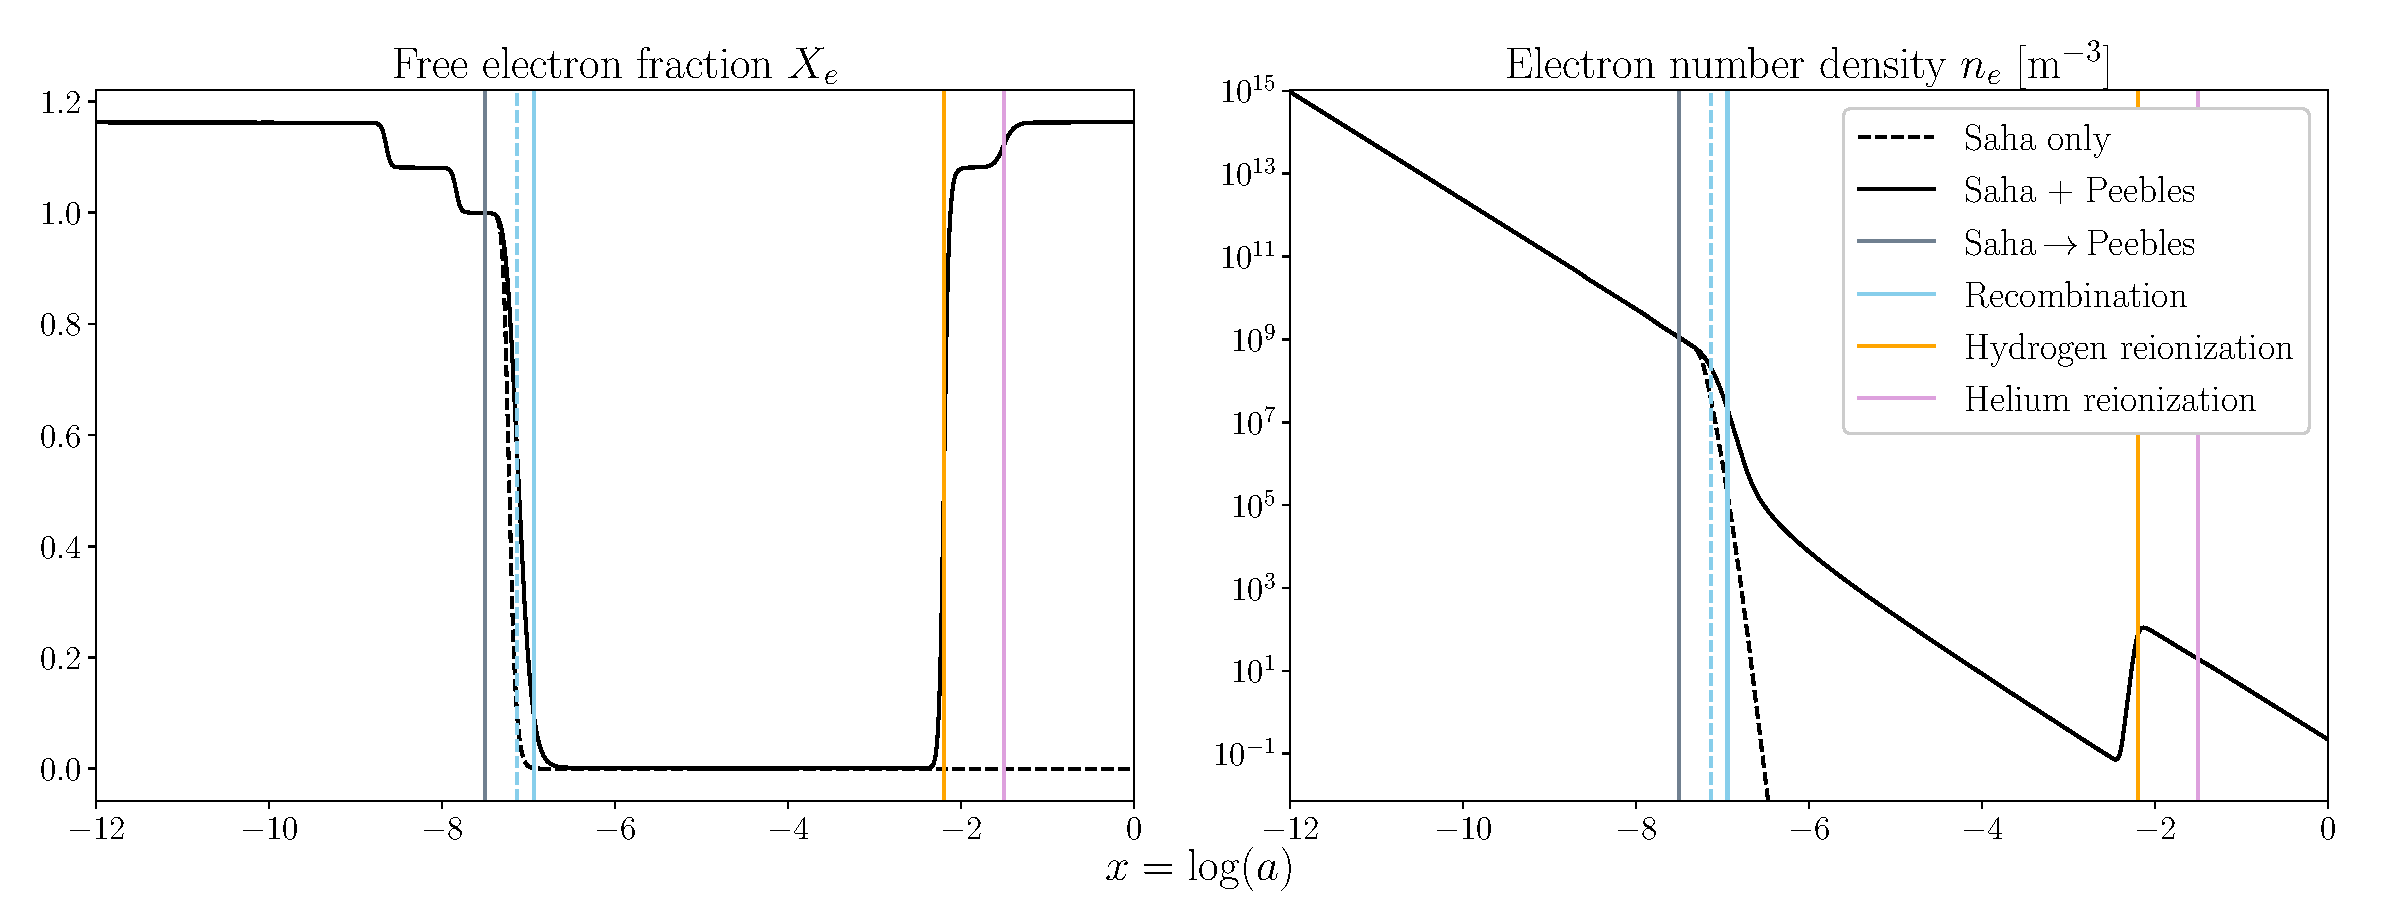
\includegraphics[width=\textwidth]{/Users/paljettrosa/Documents/GitHub/AST5220/figs/Xe_and_ne.pdf}
  \caption{The evolution of the free electron fraction $X_e$ (left) and the free electron number density $n_e$ (right) as functions of $x = \log(a)$. The dashed blue line marks the time of recombination estimated using only the Saha approximation, while the solid line shows the result from solving the Peebles equation. The significant difference illustrates the limitations of assuming equilibrium. 
  % The multiple orders of magnitude difference in $n_e$ and the sharp transitions highlight key epochs such as recombination and reionization. \colorbox{Plum}{maybe remove last sentence}
  }\label{fig:X_e and n_e}
\end{figure*}

In figure \ref{fig:X_e and n_e}, I have plotted the free electron fraction, $X_e$ (left subplot), and the electron number density, $n_e$ (right subplot), as functions of $x$. Initially, we observe that $X_e \lesssim 1.2$, reflecting a fully ionized Universe where both Hydrogen and Helium are ionized. The free electron fraction slightly exceeds 1 due to the contribution of Helium. As the Universe expands and cools, recombination progresses in stages. Around $x \approx -9$, doubly ionized Helium ($\text{He}^{++}$) captures an electron and transitions to singly ionized Helium ($\text{He}^+$). Shortly afterward, at $x \approx -8$, $\text{He}^{+}$ recombines into neutral Helium ($\text{He}$). Hydrogen recombination occurs later, around $x \approx -7$, where $X_e$ undergoes a steep decline as most free electrons combine with protons to form neutral Hydrogen. This marks Hydrogen recombination as the dominant process in determining the final ionization state of the Universe.

The impact of these recombination events is also evident in the evolution of the electron number density. During Helium recombination, $n_e$ follows the expected trend of volume dilution with no significant deviations, indicating that Helium recombination has a minimal effect on the overall number density. However, during Hydrogen recombination, $n_e$ drops by approximately four orders of magnitude, demonstrating the rapid capture of electrons by protons. A similar trend can be seen at later times: although $\text{He}^{+}$ reionization leads to an increase in the free electron fraction, its effect on the total number density is negligible compared to the large increase that occurs during the first reionization period.

By turning off reionization, I determined the freeze-out abundance of free electrons to be:
\begin{align*}
  X_e &\approx 2.7 \times10^{-4},
  \\
  n_e &\approx 5.2 \times10^{-5}\,\text{m}^{-3}.
\end{align*}
These values are consistent with standard recombination theory, which predicts a residual ionized fraction $X_e$ on the order of $10^{-3}$ to $10^{-4}$. Although this small asymptotic value is difficult to measure directly in today's highly reionized Universe, it plays an important role in our understanding of the thermal history between recombination and reionization. The presence of this residual electron population reflects both the continued existence of high-energy photons capable of reionizing hydrogen atoms and the low particle densities at late times, which reduce the likelihood of recombination events. As a result, a small fraction of electrons and protons remains unbound, preventing complete neutralization of the cosmic plasma.



\subsubsection{Optical depths}

\begin{figure*}
  \centering
  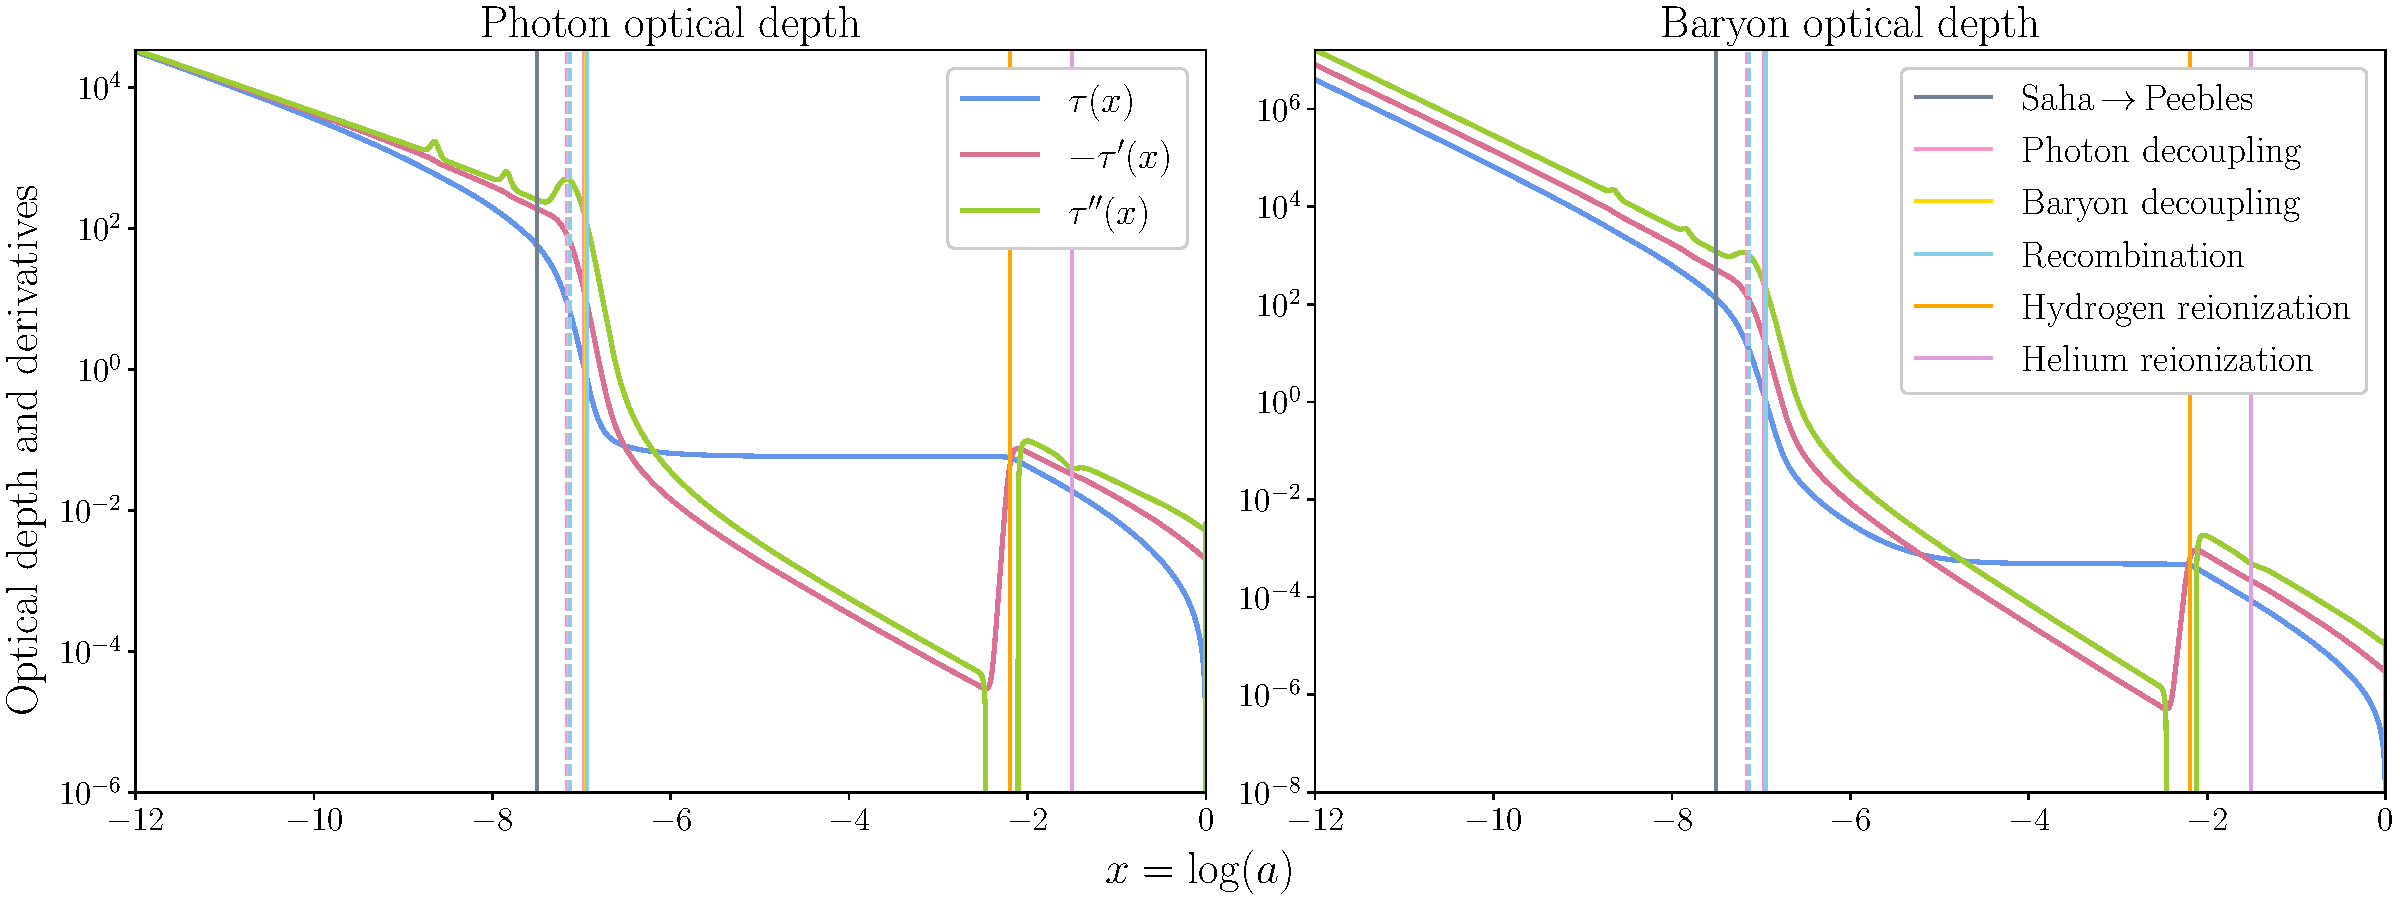
\includegraphics[width=\textwidth]{/Users/paljettrosa/Documents/GitHub/AST5220/figs/optical_depth.pdf}
  \caption{The evolution of the optical depth $\tau$ (blue), its first derivative $-\tau'$ (red), and its second derivative $\tau''$ (green) for both photons (left) and baryons (right). 
  % The bottom left subplot shows the evolutions of these quantities around decoupling and recombination, while the bottom right subplot highlights their changes during the epoch of reionization. 
  The sharp drop in $\tau$ marks photon decoupling, after which photons free-stream. In constrast, the gradual decline in $\tau_b$ indicates the prolonged influence of radiation pressure on baryons during the drag epoch. 
  % Reionization produces distinct plateaus in the optical depths, corresponding to the gradual reionization of the intergalactic medium. \colorbox{Plum}{correct? not gradual in this model?}
  }\label{fig:optical depth}
\end{figure*}

Figure \ref{fig:optical depth} shows the evolution of the photon (left) and baryon (right) optical depths (blue) and their first (red) and second derivatives (green) as functions of $x = \log (a)$. We see from the left panel that the photon optical depth $\tau$ is initially large, reflecting the fact that photons are tightly coupled to the baryon-electron plasma due to frequent Thomson scattering. Around decoupling we see a rapid drop in $\tau$, since the photons stop noticing the baryons. This is also visible from the steep negative peak in $-\tau'$, which marks the rapid decline in the scattering probability. 

The second derivative $\tau''$ provides further insight into the recombination process. In particular, we see two smaller peaks just before the dominant Hydrogen recombination, corresponding to the transitions of $\text{He}^{++} \rightarrow \text{He}^{+}$ and $\text{He}^{+} \rightarrow \text{He}$, which highlights the changes in the free electron fraction seen in figure \ref{fig:X_e and n_e}. Though subtle, these peaks indicate sudden drops in $-\tau'$, demonstrating that $X_e$ does not decrease monotonically but rather in distinct stages due to the sequential recombination of Helium and Hydrogen.

After recombination, $\tau$ levels off and remains nearly constant, meaning that photons are no longer frequently scattering. This corresponds to the transition to CMB free-streaming, where the photons released at decoupling travel largely undisturbed throughout the Universe. However, at $x \lesssim -2$ we observe a sudden increase in $-\tau'$, accompanied by a sharp drop in $\tau''$, corresponding to Hydrogen reionization. This phase is driven by ionizing radiation from early stars, which rapidly increases the free electron fraction, as reflected in the jumps in $X_e$ and $n_e$ in figure \ref{fig:X_e and n_e}. The optical depth $\tau$ then enters a plateau. A second, smaller bump at $x \approx -1.5$ arises from Helium reionization, caused by high-energy photons from quasars that fully ionize singly ionized Helium (see e.g. \cite{Helium} for updated analyzes in light of recent JWST data).

To understand the reionization plateau, consider a photon emitted at aredshift $z<z_\text{reion}$. Since most Hydrogen is ionized, it has a non-negligible probability of Thomson scattering on its way to us. This probability accumulates over time, making the optical depth larger for photons emitted further in the past. However, for photons emitted in the neutral era between recombination and reionization ($z_\text{rec} \gg z > z_\text{reion}$), the scattering probability is negligible, leading to a roughly constant optical depth in this regime. The optical depth at reionization is often a more relevant quantity than the precise redshift of reionization. From my computed spline, I found this value to be $\tau_\text{reion} = 0.0561$, which perfectly matches the Planck 2018 result: based on TT,TE,EE+lowE+lensing+BAO measurements, \cite{Planck} found $\tau_\text{reion} = 0.0561 \pm 0.0071$.

The baryon optical depth $\tau_b$ follows a similar evolution to the photon optical depth but starts from a significantly higher value. This reflects the large photon-to-baryon ratio, implying that baryons have an even shorter mean free path than photons in the tightly coupled plasma. Around decoupling, $\tau_b$ also undergoes a decline but does so more gradually due to the extended drag epoch, during which residual interactions between baryons and photons delay the onset of independent baryon motion. As seen in the photon case, Hydrogen and Helium reionization lead to a delayed but noticeable increase in $\tau_b'$, though the effect is less pronounced. Since baryons are non-relativistic, they are less affected by changes in the free electron fraction compared to photons, resulting in a weaker response to reionization.
% While photons begin free-streaming immediately, baryons remain coupled to the residual ionized plasma for a longer time, affecting the formation of the first acoustic peaks in the CMB. \colorbox{Plum}{maybe shorten/move to theory} 


\subsubsection{The visibility function}

\begin{figure}
  \centering
  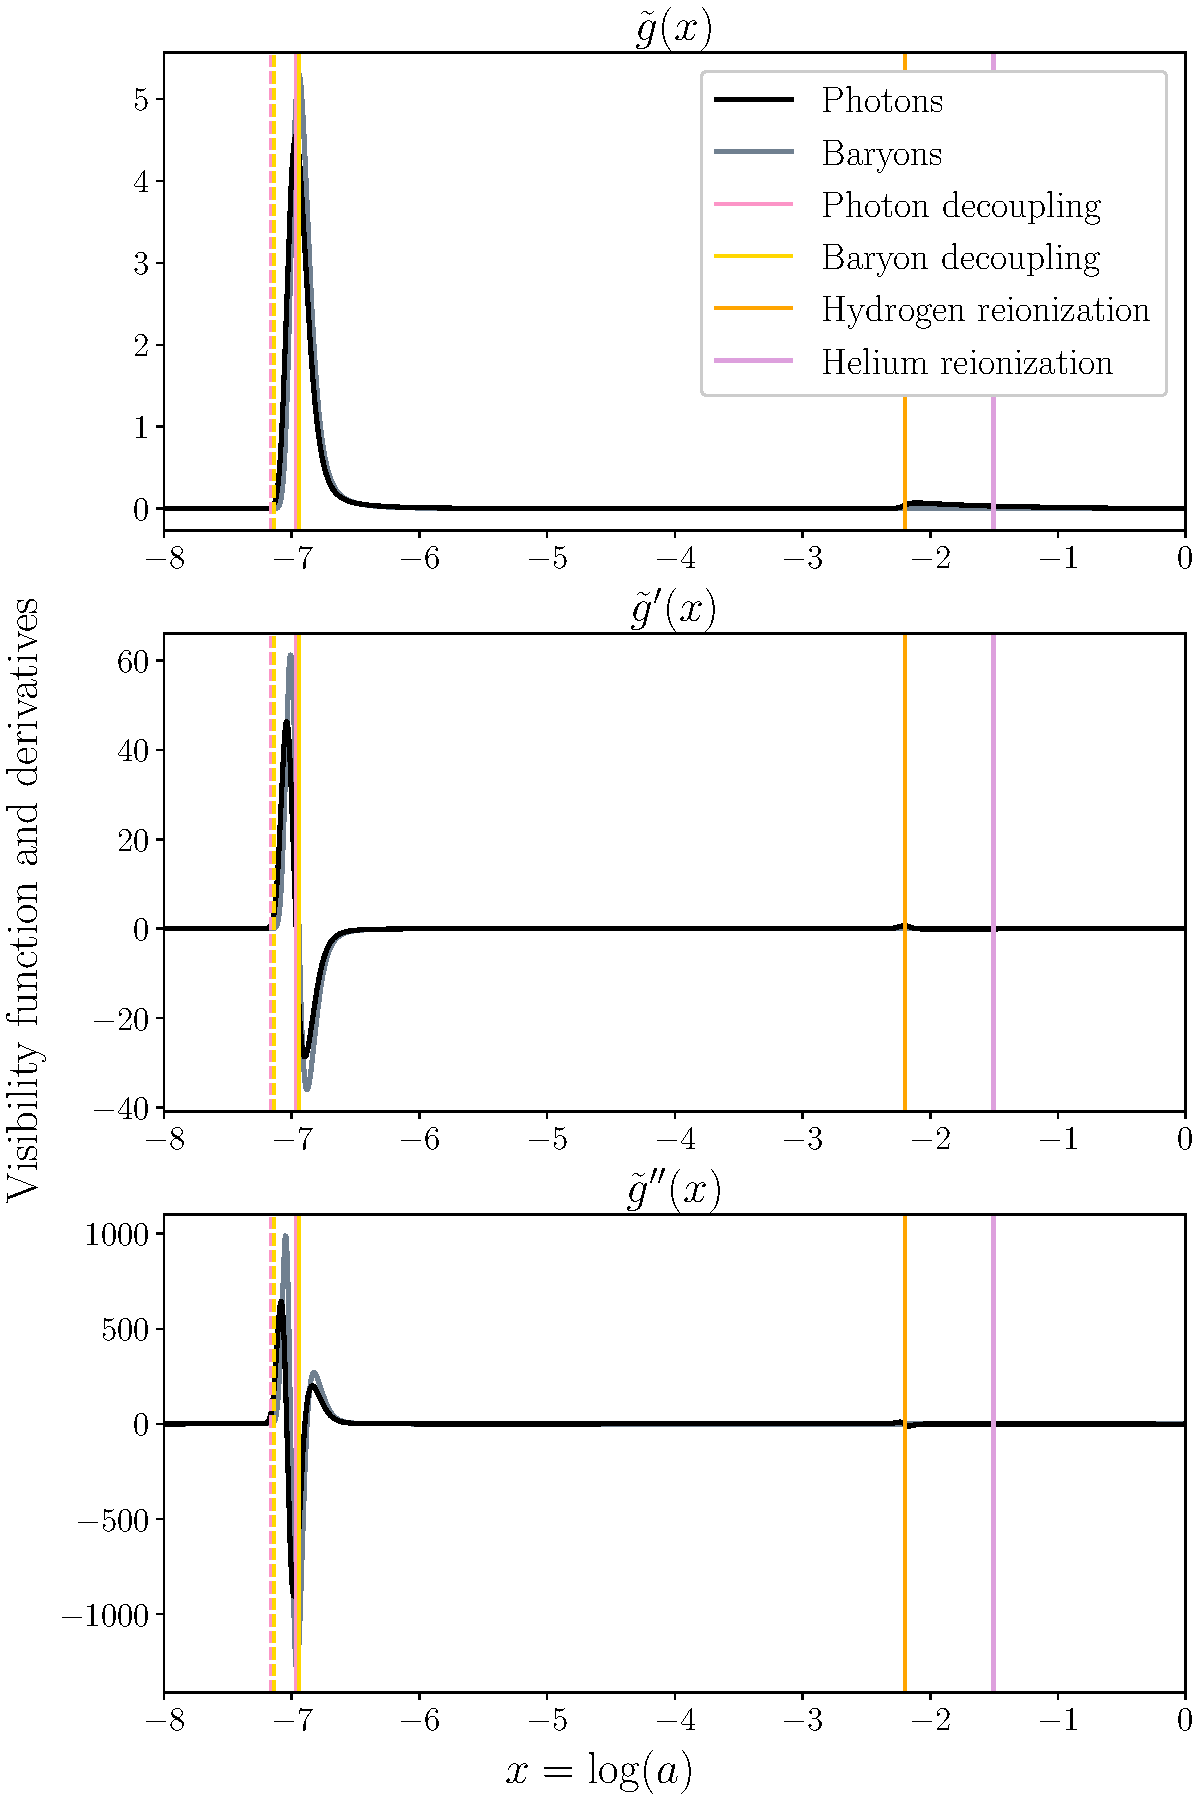
\includegraphics[width=\columnwidth]{/Users/paljettrosa/Documents/GitHub/AST5220/figs/visibility_function.pdf}
  \caption{The visibility function $\tilde{g}(x)$ (top), its first derivative $\tilde{g}'(x)$ (middle), and its second derivative $\tilde{g}''(x)$ (bottom). The sharp peak in $\tilde{g}$ defines the last scattering surface, while the first derivative's zero-crossing confirms the rapid transition. 
  % The second derivative provides insight into the smoothness of recombination, and secondary features at late times reflect reionization events. \colorbox{Plum}{maybe word differently}
  }\label{fig:visibility function}
\end{figure}

In figure \ref{fig:visibility function}, I have plotted the photon visibility function $\tilde{g}(x)$ (top), its first derivative $\tilde{g}'(x)$ (middle), and second derivative $\tilde{g}''(x)$ (bottom) as functions of $x$. The interval $x\in[-12,-8)$ has been omitted, as all these quantities remain identically zero in this range. We see that the visibility function peaks sharply around $x \approx -7$, confirming that the last scattering of CMB photons occurred near this time. 
% This peak marks the transition from frequent scattering to free-streaming and corresponds to photon decoupling.
As discussed in section \ref{subsubsec: II theory optical depth}, the width of the peak in $\tilde{g}(x)$ reflects the thickness of the last scattering surface, while the zero-crossing of $\tilde{g}'(x)$ indicates the time of steepest decline in scattering probability. 
% The strong dip in $\tilde{g}''(x)$ around $x \approx -7$ quantifies the sharpness of this transition, and verifying the shape of $\tilde{g}''(x)$ is important for ensuring the accuracy of later computations, particularly the source function used in the line-of-sight integration.

At later times, around $x \lesssim -2$, Hydrogen reionization causes a secondary, broader increase in $\tilde{g}(x)$, reflecting the renewed interaction between photons and free electrons. However, this increase is significantly smaller than at recombination, indicating that only a fraction of CMB photons were re-scattered during this epoch. The visibility function barely changes during the subsequent reionization of singly ionized Helium to doubly ionized Helium, as expected from the negligible impact of this process on the optical depths and their first derivatives.



\subsubsection{Important time stamps and horizons}

\begin{table*}
  \caption{Table of key cosmological time stamps, showing photon and baryon decoupling, the changes that occur inbetween (the drag epoch), and recombination, along with their corresponding redshifts, cosmic times, conformal times (particle horizons), and sound horizons. The Saha-only results differ significantly from the full solution, underestimating recombination time due to its equilibrium assumption.} 
  %The sound horizon at recombination sets the scale for acoustic peaks in the CMB and BAO in large-scale structure. \colorbox{Plum}{fact check} \colorbox{Plum}{add Planck values!}}             % title of Table
  \label{table:time stamps decoupling}    % is used to refer this table in the text
  \centering                          % used for centering table
  \begin{tabular}{| c || c || c | c | c | c |}        % centered columns (4 columns)
  \hline                % inserts double horizontal lines
  Quantity & Method & Photon decoupling & Baryon decoupling & Drag epoch & Recombination \\    % table heading 
  \hline\hline                        % inserts single horizontal line
  \multirow{2}{*}{$x$}       & Saha only       & \hspace{4.5pt}$-7.16$  & \hspace{4.5pt}$-7.14$     & \hspace{4.5pt}$0.02$        & \hspace{4.5pt}$-7.13$   \\      
  \cline{2-6}
                           & Saha + Peebles  & \hspace{4.5pt}$-6.97$  & \hspace{4.5pt}$-6.95$     & \hspace{4.5pt}$0.02$        & \hspace{4.5pt}$-6.94$   \\      
  \hline 
  \multirow{2}{*}{$z$}       & Saha only       & \hspace{-4pt}$1291.70$ & \hspace{-4pt}$1260.11$    & \hspace{-7pt}$-31.59$       & \hspace{-4pt}$1249.29$ \\
  \cline{2-6}
                           & Saha + Peebles  & \hspace{-4pt}$1064.44$ & \hspace{-4pt}$1037.76$    & \hspace{-7pt}$-26.68$       & \hspace{-4pt}$1033.21$ \\
  \hline 
  \multirow{2}{*}{$t$ [kyr]} & Saha only       & \hspace{1pt}$279.19$   & \hspace{1pt}$291.19$      & \hspace{-0.5pt}$11.99$        & \hspace{1pt}$295.48$    \\
  \cline{2-6}
                           & Saha + Peebles  & \hspace{1pt}$387.17$   & \hspace{1pt}$404.02$      & \hspace{-0.5pt}$16.85$      & \hspace{1pt}$407.01$    \\
  % \hline 
  % $\eta/c$ (Saha, TODO) & $934.94\,$Myr & \hspace{6pt}$949.53\,$Myr   & \hspace{0pt}$14.59\,$Myr  & \hspace{0pt}$14.59\,$Myr \\ 
  % \cline{2-6}
  % $\eta/c$ (numerical)  & $934.94\,$Myr & \hspace{6pt}$949.53\,$Myr   & \hspace{0pt}$14.59\,$Myr  & \hspace{0pt}$14.59\,$Myr TODO \\
  \hline 
  \multirow{2}{*}{$\eta$ [Mpc]} & Saha only       & \hspace{1pt}$246.80$   & \hspace{1pt}$251.49$      & \hspace{4.5pt}$4.69$        & \hspace{1pt}$253.14$    \\ 
  \cline{2-6}
                           & Saha + Peebles  & \hspace{1pt}$285.49$   & \hspace{1pt}$290.92$      & \hspace{4.5pt}$5.43$        & \hspace{1pt}$291.87$    \\ 
  \hline 
  \multirow{2}{*}{$s$ [Mpc]} & Saha only       & \hspace{1pt}$128.90$   & \hspace{1pt}$131.09$      & \hspace{4.5pt}$2.19$        & \hspace{1pt}$131.85$    \\ 
  \cline{2-6}
                           & Saha + Peebles  & \hspace{1pt}$146.66$   & \hspace{1pt}$149.10$      & \hspace{4.5pt}$2.44$        & \hspace{1pt}$149.53$    \\
  \hline                                   %inserts single line
  \end{tabular}
\end{table*}

Table \ref{table:time stamps decoupling} presents the computed values of $x$, redshift $z$, cosmic time $t$, conformal time (particle horizon) $\eta$, and sound horizon $s$ corresponding to photon and baryon decoupling, the changes that occured during the drag epoch in between the two, as well as recombination. The values are given both for calculations using only the Saha approximation and for the more accurate approach that includes the full Peebles equation. As expected, photon decoupling (where $\tau$ falls to unity) and recombination (when $X_e$ drops below 0.1) occur at nearly identical times. This is because photons cease scattering once neutral Hydrogen forms, making the two processes tightly linked. However, recombination happens slightly later because a residual fraction of free electrons persists even after photons transition to free-streaming. Baryon decoupling occurs between the two, as evident from figures \ref{fig:optical depth} and \ref{fig:visibility function}. 
% This delay arises because even after photons stop scattering frequently, baryons still experience residual drag from the remaining photon-baryon interactions, which only fully cease after the drag epoch.

The Saha approximation alone predicts earlier times of recombination and decoupling, consistent with the steeper drop in the free electron fraction observed in figure \ref{fig:X_e and n_e}. This discrepancy arises because the Saha equation assumes instantaneous thermal equilibrium, meaning ionization and recombination are treated as occurring instantaneously when crossing equilibrium thresholds. However, in reality, recombination is a non-equilibrium process, as captured by the Peebles equation, which accounts for the slower capture of electrons by protons in an expanding universe.

The difference in sound horizons between the two approaches highlights the impact of an earlier recombination. Since sound waves in the tightly coupled photon-baryon plasma define the characteristic scale of acoustic oscillations, an earlier recombination results in a slightly smaller sound horizon. This has direct consequences for the CMB anisotropy spectrum, as the first acoustic peak corresponds to the largest mode that fits within the sound horizon at decoupling. A smaller sound horizon shifts the peak positions and alters the angular scale of the acoustic features in both the CMB power spectrum and the BAO in the matter power spectrum. This clearly demonstrates the necessity of using the Peebles equation to accurately model recombination, as relying on the Saha approximation alone leads to artificially early decoupling and incorrect predictions for the CMB and BAO scales.

% \colorbox{Plum}{rename section?}


\begin{figure}
  \centering
  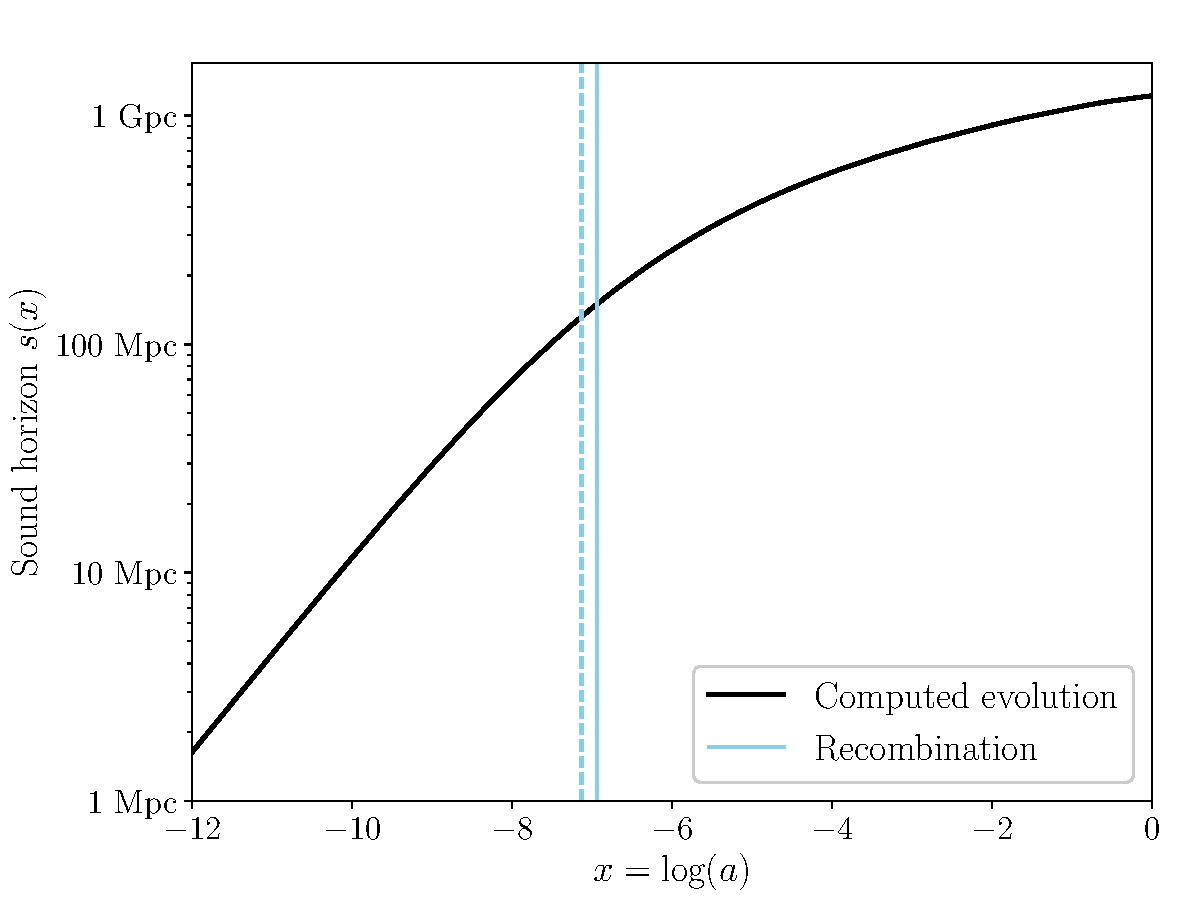
\includegraphics[width=\columnwidth]{/Users/paljettrosa/Documents/GitHub/AST5220/figs/sound_horizon.pdf}
  \caption{The evolution of the sound horizon $s(x)$ as a function of $x = \log(a)$. The rapid early growth reflects the high sound speed in the tightly coupled photon-baryon plasma, while the flattening at recombination marks the transition to the matter era.}\label{fig:sound horizon}
\end{figure}

Figure \ref{fig:sound horizon} illustrates the evolution of the sound horizon $s(x)$, with the estimated time of recombination marked to highlight where its growth gets stunted. In the early Universe, the sound horizon increases rapidly due to the high sound speed in the tightly coupled photon-baryon fluid. This is a direct consequence of the nearly relativistic equation of state of the plasma, where the sound speed $c_s$ remains close to $c/\sqrt{3}$. However, around recombination, the pressure support from photons is significantly reduced, allowing matter to cluster more freely and leading to a decrease in the sound speed. Consequently, the growth of the sound horizon flattens out as baryons decouple from photons and begin falling into dark matter potential wells, setting the scale of BAO in the later Universe.

In \cite{Planck}, the estimated redshifts of photon and baryon decoupling are $z_s = 1089.92\pm0.25$ and $z_\text{drag} = 1059.94\pm0.30$, respectively, based on $1\sigma$ constraints from TT,TE,EE+lowE+lensing measurements. The corresponding sound horizons are $r_s = 144.43\pm0.26\,\text{Mpc}$ and $r_\text{drag} = 149.09\pm0.26\,\text{Mpc}$. My computed values for $z_s$ and $z_\text{drag}$ are systematically lower, although the resulting sound horizons—particularly $r_\text{drag}$—are in good agreement with the Planck results. This discrepancy in redshift does not necessarily indicate a numerical error but rather reflects a key difference in methodology: while I have computed these quantities using a fixed fiducial cosmology, Planck reports statistically inferred values obtained by fitting a cosmological model to observational data. Differences in how reionization is handled (e.g., the choice of $z_\text{reion} = 8$ in my calculations vs. Planck's $z_\text{reion} = 7.64$) could also slightly shift estimated parameters.

Using the value for the particle horizon at photon decoupling presented in table \ref{table:time stamps decoupling} (Saha + Peebles approach) and the present-day particle horizon from table \ref{table:time stamps} (numerical value), the comoving distance to the last scattering surface is found to be $\chi_{s} \approx 13904.51\,$Mpc. With my computed sound horizon at decoupling of $r_s \approx 146.66\,$Mpc, this gives an angular acoustic scale of $100\theta_{s} \approx 1.0548$. This is slightly larger than the Planck result of $100\theta_{s} = 1.0411\pm0.0003$, falling outside their reported uncertainty. However, it should be noted that I have not been able to estimate the uncertainty of my estimate, and that the Planck value could fall within this range. Potential sources of this uncertainty include the finite resolution of the numerical integration, the choice of interpolation method for the visibility function, and approximations made in the recombination model.

\colorbox{Plum}{TODO: maybe change/remove last part}



\subsubsection{Baryon temperature evolution}

\begin{figure}
  \centering
  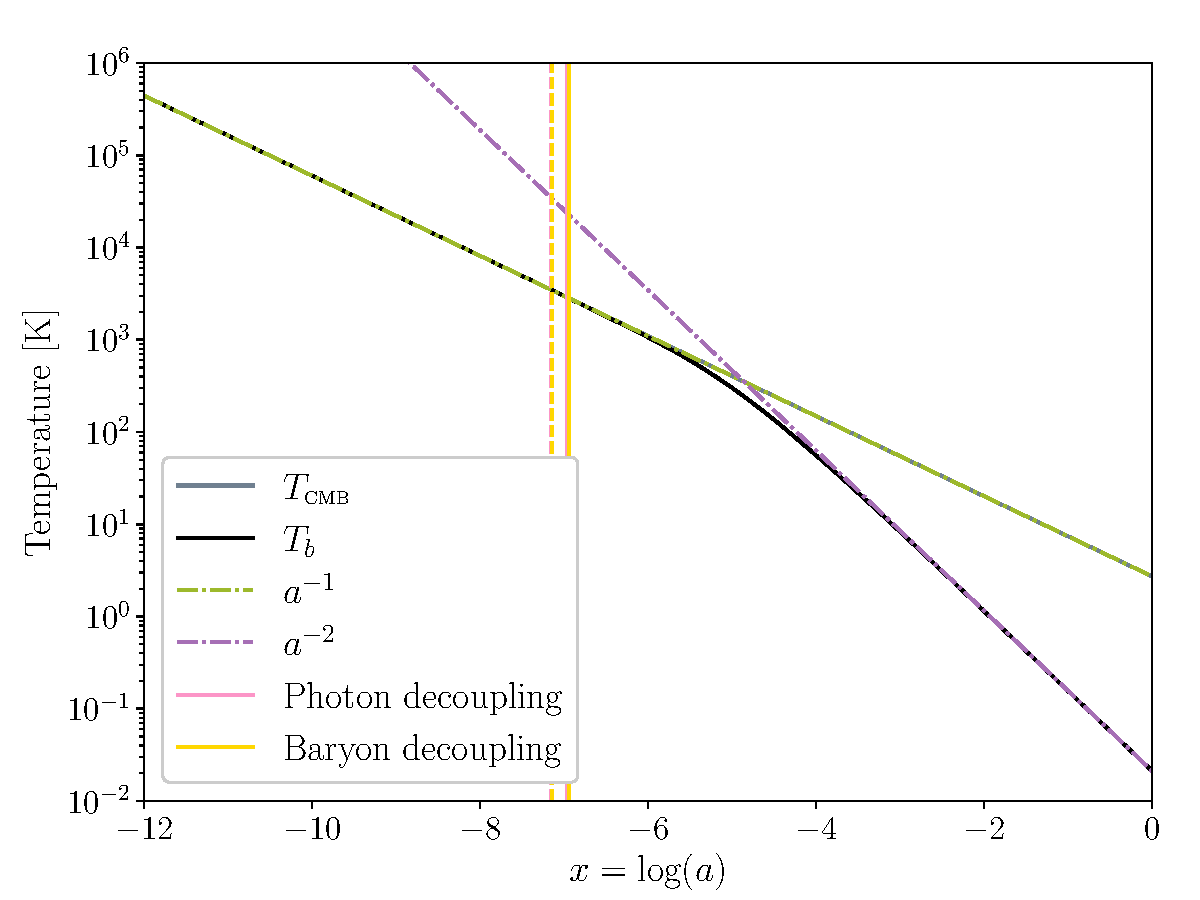
\includegraphics[width=\columnwidth]{/Users/paljettrosa/Documents/GitHub/AST5220/figs/photon_baryon_temp.pdf}
  \caption{The evolution of the baryon temperature $T_b(x)$ (black) compared to the photon temperature $T_\text{CMB}(x)$ (grey). The two temperatures track each other closely before recombination due to strong Thomson scattering. Some time after decoupling, baryons start to cool adiabatically as $T_b \propto a^{-2}$ (purple dashed line), while photons continue to cool as $T_\text{CMB} \propto a^{-1}$ (green dashed line).}\label{fig:baryon temperature}
\end{figure}

Figure \ref{fig:baryon temperature} illustrates the evolution of the baryon temperature $T_b(x)$ (black line) compared to the photon (CMB) temperature $T_\text{CMB}(x)$ (grey line). Before recombination the baryon temperature closely follows the photon temperature due to strong Thomson scattering between electrons and CMB photons, which ensures thermal equilibrium. In this regime, both temperatures scale as $T \propto a^{-1}$, as expected for a relativistic plasma. However, 
% after recombination, photon interactions become infrequent, allowing the baryons to cool adiabatically as $T_b \propto a^{-2}$, while the CMB continues to cool following the radiation-like scaling of $T_\text{CMB} \propto a^{-1}$.
% In figure \ref{fig:optical depth} we saw a sharp decrease in the optical depth around decoupling, due to Thomson scattering becoming inefficient after the free electron fraction drops. As a result, baryons are no longer in thermal equilibrium with photons, and the two temperatures begin to diverge. 
baryons begin to cool independently some time after recombination, around $x\approx-6$. At this point, the baryon temperature transition from the radiation-like scaling to an adiabatic evolution, where $T_b \propto a^{-2}$, since the baryons no longer receive energy from photons and instead evolve as a non-relativistic gas in an expanding universe. This is directly linked to the drop in optical depth observed in figure \ref{fig:optical depth}. The delay between decoupling and the point where the two diverge explains why $\tau_b$ declines more gradually than $\tau$, extending the impact of photon pressure beyond the formal decoupling time. 

I found the baryon temperature to be $T_{b0} \approx 21\,\text{mK}$, which is only about $\sim 7-8\%$ of the measured CMB temperature today. This result is consistent with theoretical expectations, given the $a^{-2}$ scaling of $T_b$ after $x\approx 6$ compared to the $a^{-1}$ scaling of $T_\text{CMB}$. However, unlike the CMB temperature, which follows a nearly perfect blackbody distribution with only small-scale anisotropies encoding information about early-universe physics, the baryon temperature is not a meaningful global quantity today. This is because matter has strongly clustered since decoupling, leading to highly non-linear structure formation. Most of the baryonic content is no longer in a diffuse, cold state, but concentrated into dense regions such as stars, galaxies, and the hot intergalactic medium. There are very few regions of truly diffuse baryonic gas with temperatures as low as the mean value presented here, though such cold gas remains an active area of research in extragalactic astronomy (see e.g., \cite{tumlinson2017circumgalactic} and \cite{nelson2020cold} about the cold circumgalactic medium).

The temperature deviation between photons and baryons introduces a minor correction to the photon-baryon sound speed, which in principle affects the evolution of acoustic oscillations. However, since recombination is complete before $T_b$ and $T_\text{CMB}$ significantly diverge, this effect is minimal. For precision calculations of the CMB power spectrum, including the evolution of $T_b$ can slightly refine the modeling of BAO, but its impact on large-scale anisotropies will likely remains small, as mentioned in section \ref{subsubsec: II theory baryon temp}.








\section{Milestone III: Perturbations}\label{sec: milestone III}
Having established the background evolution of the universe and the recombination history in the previous milestones, I now turn to the evolution of cosmological perturbations, which describe how small fluctuations in density and temperature grew from the early Universe into the large-scale structures we observe today. This step is essential for understanding the formation of CMB anisotropies, as well as the distribution of galaxies and clusters in the late Universe. 

In this milestone, I numerically solve the Einstein-Boltzmann equations in linear perturbation theory to track the evolution of cosmological perturbations in photons, neutrinos, baryons, and cold dark matter. These are computed across different Fourier modes to obtain time-dependent solutions for key quantities such as density and velocity perturbations, temperature anisotropies, and gravitational potentials. To manage numerical instabilities at early times, I implement the tight-coupling approximation. The resulting solutions form the basis for computing the CMB power spectrum in the next milestone, enabling direct comparison between theory and observation.

\subsection{Theoretical framework}\label{subsec: III theory}

% \begin{enumerate}
%   \item [1.] Introduce the concept of metric perturbations by writing up the perturbed line element $ds^2$, and explain that the Einstein equations for scalars, vectors and tensors don't mix at linear order and can therefore be treated separately. I will mostly focus on scalar fluctuations and the associated density perturbations. Vector perturbations aren't produced by inflation and even if they were, they would decay quickly with the expansion of the Universe. Tensor perturbations (gravitational waves) are an important prediction of inflation and I will get back to them in the next milestone. 
%   \item [2.] Explain that we use the Newtonian gauge because we then can apply some of our Newtonian intuition, and introduce the potentials $\Psi$ and $\Phi$. 
%   \item [3.] Explain that the perturbation equations we end up with are going to be coupled linear partial differential equations, which are not trivial in real space, hence why we go to Fourier space. Explain that we go from spatial variables $v^i$ to wave vector components $k^i$, and that $\nabla u(x)\to i\vec{k}\tilde{u}(k)$ as we move to Fourier space.
%   \item [4.] Introduce the perturbed Einstein-Boltzmann equation (the Boltzmann equation in general relativity that we introduced in the previous milestone) for photons, by stating the geodesic equation in a perturbed universe. Use this to show the momentum perturbations for photons today (subscript 0) as function of values at recombination (subscript rec): 
%   \begin{equation}
%     \left(\frac{\delta p}{p}\right)_0 = \left(\frac{\delta p}{p}\right)_\text{rec} + \left(\Psi_\text{rec} - \Psi_0\right) + \int_{t_\text{rec}}^{t_0}\left[\frac{\partial\Psi}{\partial t} - \frac{\partial \Phi}{\partial t} \right]\,dt,
%   \end{equation}
%   and identify and explain the Sachs-Wolfe and Integrated Sachs-Wolfe effects. Explain what these mean, and how important they are for understanding CMB anisotropies.
%   \item [5.] Explain that by introducing perturbations in the temperature 
%   \begin{equation}
%     T=\overline{T}(1+\Theta(t,\vec{x},p,\hat{p})),
%   \end{equation}
%   and thus in the distribution function for photons (expand this in the $\Theta\ll1$ limit) we end with the Boltzmann equation with the background subtracted.
%   \item [5.] Finally arrive at the explicit expressions for the photon temperature multipoles, using multipole expansions. Explain where these come from, and state the general expressions.
%   \item [6.] Explain what the monopole, dipole and quadrupole represent.
%   \item [7.] Explain how and why we truncate the Boltzmann hierarchies of infinite equations.
%   \item [8.] Explain the concept of polarization of photons, and how the polarization spectra can be used to constrain parameters. 
%   \item [9.] State the explicit polarization expressions in the problem description, and explain that we will further analyze the concept itself, the E-modes and B-modes (explain briefly what these are) and their spectra in the next milestone.
%   \item [10.] Explain that this is very similar to the photon situation, but without polarization and a collision term. Explain also that neutrinos in reality have mass, and that it becomes significantly more complicated if we include this, hence why we ignore it.
%   \item [11.] State the explicit expressions for the neutrino multipoles, and explain them.
%   \item [12.] Derive the explicit expressions for cold dark matter density perturbations and velocity. See the lecture notes.
%   \item [13.] Derive the explicit expressions for baryon density perturbations and velocity. See the lecture notes.
%   \item [14.] Make sure to mention the interactions we can ignore/must include for baryons, hence why the collision term is not zero.
%   \item [15.] Explain that the nonzero metric elements are
%   \begin{align}
%     g_{00} &= -\left(1+2\Psi \right),
%     \\
%     g_{ij} &= a^2\left(1+2\Phi \right)\delta_{ij},
%   \end{align}
%   and that, since the potentials $\Psi$ and $\Phi$ are small, the inverse metric components are
%   \begin{align}
%     g^{00} &= -\frac{1}{1+2\Psi} \simeq -1+2\Psi,
%     \\
%     g^{ij} &= \frac{1}{a^2\left(1+2\Phi \right)}\delta_{ij} \simeq a^{-2}\left(1-2\Phi\right)\delta_{ij}.
%   \end{align}
%   \item [16.] Move on to explain that after computing the Christoffel symbols, the Ricci tensor and scalar, and the Einstein tensor, we can move on to the general relativistic expression for the energy momentum tensor in the Boltzmann formalism:
%   \begin{equation}
%     T_\nu^\mu = \frac{g}{(2\pi)^3}\int\frac{dP_1dP_2dP_3}{\sqrt{-\text{det}\,g}}\frac{P^\mu P_\nu}{P^0}f,
%   \end{equation}
%   where $P^\mu=dx^\mu/d\lambda$ is the 4-momentum and $\text{det}\,g$ is the determinant of the metric $g_{\mu\nu}$. Show the approximate expression for this, using that it is diagonal, and explain that we can compute the $\mu=0$, $\nu=0$ component with $f=\overline{f}+\delta f$ to get
%   \begin{align}
%     \left(T_0^0\right)_\gamma &= -\overline{\rho}_\gamma\left(1+4\Theta_0\right),
%     \\
%     \left(T_0^0\right)_\nu &= -\overline{\rho}_\nu\left(1+4\mathcal{N}_0\right),
%     \\
%     \left(T_0^0\right)_\text{CDM} &= -\overline{\rho}_\text{CDM}\left(1+\delta_\text{CDM}\right),
%     \\
%     \left(T_0^0\right)_b &= -\overline{\rho}_b\left(1+\delta_b\right),
%   \end{align}
%   \item [17.] Explain then how this leads to the expressions for $\Phi'$ and $\Psi$ stated in the problem description. 
%   \item [18.] Briefly explain what inflation is, why we need it (primarily horizon and flatness problem), and explain how this affects our initial conditions.
%   \item [19.] State the initial conditions we will use, and explain where each of them come from.
%   \item [20.] Explain what the tight-coupling regime is, why it introduces a problem for solving the full set of equations, and how we will combine the solution from this regime with the solution at later times to describe the entire process. 
%   \item [21.] Derive the relevant expressions from the problem description, and explain where they come from and why they are more numerically stable.
%   \item [22.] Tie the initial conditions together with the higher order $\ell\geq2$ multipole moments.
% \end{enumerate}

% % Points 1-3 are for subsection 1, points 4-9 for subsection 2, points 10 and 11 for subsection 3, 12 for subsection 4, 13 and 14 for subsection 5, 15-17 for subsection 6, 18 and 19 for subsection 7, and points 20-22 for subsection 8. 

% % Can you write subsection 8 about the tight-coupling regime? Make sure to include points 20-22. Be concise and thorough, and match my writing style from the previous milestones.

\subsubsection{Metric perturbations}

The perturbed Einstein equations for scalars, vectors, and tensors decouple at linear order, allowing us to study them separately. In this work, I primarily focus on scalar perturbations, which correspond to density fluctuations and are responsible for structure formation. Vector perturbations (vorticity) are not generated by inflation and decay rapidly due to cosmic expansion, hence they are irrelevant when computing the CMB. Furthermore, tensor perturbations (gravitational waves) are a key prediction of inflation and is therefore a topic I revisit in the next milestone. 

To simplify the perturbation equations, I work in the Newtonian gauge, where the metric is diagonal:
\begin{equation}
ds^2 = - \,(1 + 2\Psi)\,dt^2 + a^2 (1 + 2\Phi)\, \delta_{ij}\, dx^i dx^j.
\end{equation}
Here, $\Psi$ and $\Phi$ are the gravitational potentials, which describe scalar perturbations to the metric and play analogous roles to the Newtonian potential in classical gravity. This is another perk of working in the Newtonian gauge, as it allows for more intuitive physical interpretation while keeping the full relativistic structure of general relativity. More specifically, $\Psi$ represents the perturbation to the time-time component of the metric and acts as the gravitational potential experienced by non-relativistic particles, while $\Phi$ appears in the spatial metric perturbations and affects the expansion of space. 


The perturbation equations take the form of coupled partial differential equations in real space, which are not trivial to solve. To simplify the problem, we transform them into Fourier space, where they become a system of ordinary differential equations for each wave mode. 
% This is justified by the linearity of the system, allowing each mode to evolve independently.  
In Fourier space, spatial derivatives transform as:  
\begin{equation}
\nabla u(x) \rightarrow i \vec{k} \tilde{u}(k),
\end{equation}
where $\vec{k}$ is the comoving wave vector of the perturbation. This Fourier decomposition allows us to track the evolution of perturbations across different scales and study their behavior from superhorizon to subhorizon regimes. 

\subsubsection{Photons}\label{subsubsec: III theory photons}
The evolution of CMB anisotropies is governed by perturbations in the photon distribution function. Since photons are massless, they follow null geodesics in a perturbed metric. For a photon with four-momentum $P^\mu$ and energy $E=p$, expanding the Christoffel symbols in the geodesic equation leads to: 
\begin{align}
&\frac{dP^0}{d\lambda} + \Gamma^0_{\mu\nu} P^\mu P^\nu = 0 \\
\Rightarrow\hspace{5pt} &\frac{dp}{dt} = \frac{1}{P_0}\frac{dp}{d\lambda} \simeq -p\left[H + \frac{\partial \Phi}{\partial t} + \frac{\partial \Psi}{\partial x^{i}}\frac{\hat{p}^{i}}{a}\right].
\end{align}
\colorbox{Plum}{show this?} This equation describes how the photon energy changes due to both cosmic expansion (the Hubble term $H$) and metric perturbations. Integrating from recombination to today gives the perturbation to the photon energy in terms of its initial value: 
\begin{equation}
\left(\frac{\delta p}{p}\right)_0 = \left(\frac{\delta p}{p}\right)_{\text{rec}} + \left(\Psi_{\text{rec}} - \Psi_0\right) + \int_{t_{\text{rec}}}^{t_0} \left[\frac{\partial\Psi}{\partial t} - \frac{\partial \Phi}{\partial t} \right] dt. \label{eq: photon momentum}
\end{equation}


Eq. \eqref{eq: photon momentum} encodes two key effects that shape CMB anisotropies. The first of these is the Sachs-Wolfe effect: the gravitational redshift of photons due to metric perturbations at the last scattering surface, corresponding to the term $(\Psi_{\text{rec}} - \Psi_0)$. More specifically, this represents the change in the gravitational potential from recombination to today. Furthermore, the last term represents the time variation of the metric perturbations $(\partial_t \Psi - \partial_t \Phi)$, which affects photons' energies as they travel through evolving potential wells. This is called the integrated Sachs-Wolfe (ISW) effect, and is most important in the late Universe when dark energy becomes significant. 
% These effects contribute to large-scale temperature fluctuations in the CMB, directly imprinting information about early-universe physics and cosmic structure formation.

To describe perturbations in the CMB systematically, we introduce the photon temperature perturbation, defined as:
\begin{equation}
T = \overline{T} (1 + \Theta),
\end{equation}
where $\Theta = \delta T/\overline{T}$ represents small deviations from the mean photon temperature. This perturbation generally depends on time, space, the magnitude, and direction of the photon momentum. However, since Thomson scattering only affects the direction of the photon momentum to first order, we can express the perturbation as $\Theta(t, \vec{x}, \hat{p})$, eliminating explicit dependence on $p$. Furthermore, expanding the distribution function for photons in the limit $\Theta \ll 1$ gives:
\begin{equation}
f = \frac{1}{e^{p/\overline{T}(1-\Theta)}-1} \simeq \overline{f} + \Theta p\frac{\partial\overline{p}}{\partial p} \Theta,
\end{equation}
where 
\begin{equation}
  \overline{f} = \frac{1}{e^{p/\overline{T}}-1}.
\end{equation}
Since the chemical potential $\mu=0$ for photons, this follows directly from the Bose-Einstein distribution (eq. \eqref{eq: distribution}). Subtracting the background evolution from the full Boltzmann equation \eqref{eq: Boltzmann} leads to the first-order perturbed Boltzmann equation for photons:
\begin{equation}
\frac{df}{d\lambda} = -p^2\frac{\partial\overline{f}}{\partial p}\left[\frac{\partial{\Theta}}{\partial t} + \frac{\partial{\Theta}}{\partial x^{i}}\frac{\hat{p}^{i}}{a} + \left(\frac{\partial{\Phi}}{\partial t} + \frac{\partial{\Psi}}{\partial x^{i}}\frac{\hat{p}^{i}}{a} \right) \right] = C[f]. \label{eq: Boltzmann photons}
\end{equation}
\colorbox{Plum}{show this more explicitly?} 

% As discussed extensively in the previous milestone, the dominant interaction term for photons is Thomson scattering with free electrons. \colorbox{Plum}{too repetitive?} 
If we ignore polarization and the angular dependence of the Thomson scattering cross section, the collision to first order in perturbation theory simplifies to
\begin{equation}
  C[f] = -p^2\frac{\partial\overline{f}}{\partial p}n_e\sigma_\text{T}\left(\Theta_0 - \Theta + \hat{p}\cdot\vec{v}_b \right). \label{eq: collision photons}
\end{equation}
Here, $\vec{v}_b$ is the baryon velocity, which describes how fast electrons (and protons) are moving, and
\begin{equation}
  \Theta_0 = \frac{1}{4\pi}\int\Theta\,d\Omega_{\hat{p}} = \frac{1}{2}\int_{-1}^{1}\Theta\,d\mu, 
\end{equation}
is the monopole moment of the photon distribution, which describes the local temperature averaged over all directions. The integration variable $\mu$ is simply the cosine of the angle between the wavevector $\vec{k}$ and the photon direction:
\begin{equation}
  \mu = \hat{p}\cdot\frac{\vec{k}}{k}.
\end{equation}
Thus, inserting this into eq \eqref{eq: Boltzmann photons} we arrive at the perturbed Boltzmann equation for photons:
\begin{equation}
  \frac{\partial{\Theta}}{\partial t} + \frac{\partial{\Theta}}{\partial x^{i}}\frac{\hat{p}^{i}}{a} + \left(\frac{\partial{\Phi}}{\partial t} + \frac{\partial{\Psi}}{\partial x^{i}}\frac{\hat{p}^{i}}{a} \right) = n_e\sigma_\text{T}\left(\Theta_0 - \Theta + \hat{p}\cdot\vec{v}_b \right).
\end{equation}
This equation tells us that when Thomson scattering is efficient, photons from different directions have the same temperature, enforcing $\Theta\approx\Theta_0$ locally.

Since CMB perturbations are naturally described in Fourier space, it is convenient to make use of $\vec{k}$ and $\mu$. The baryon velocity is curl-free, so in Fourier space it simplifies to 
\begin{equation} 
  \vec{v}_b = iv_b \frac{\vec{k}}{k}. 
\end{equation} 
With this, the Boltzmann equation transforms into
\begin{equation} 
  \frac{\partial \Theta}{\partial t} + \frac{ik\mu}{a} \Theta + \left(\frac{\partial\Phi}{\partial t} + \frac{ik\mu}{a} \Psi \right) = n_e\sigma_T \hspace{-1pt}\left(\Theta_0 \hspace{-1pt}-\hspace{-1pt} \Theta \hspace{-1pt}+ \hspace{-1pt}i\mu v_b - \frac{3\mu^2 - 1}{4} \Pi \right)\hspace{-1pt}, \label{eq: Boltzmann photons Fourier}
\end{equation} 
where the additional term 
\begin{equation}
  \Pi = \Theta_2 + \Theta_0^P + \Theta_2^P, \label{eq: Pi}
\end{equation}
accounts for the angular dependence of Tomson scattering through the temperature quadrupole $\Theta_2$, and CMB polarization through the polarization monopole $\Theta_0^P$ and quadrupole $\Theta_2^P$.
% where the additional term 
% \begin{equation}
%   \Pi = \Theta_2 = -\frac{1}{2}\int_{-1}^{1}\Theta \frac{3\mu^2-1}{2}\,d\mu, \label{eq: Pi old}
% \end{equation}
% accounts for the angular dependence of Tomson scattering. 
% and CMB polarization, although the latter is ignored here. 
% \colorbox{Plum}{TODO: introduce w/ polarization here?} 
% Expanding in Legendre multipoles will eventually give us a coupled hierarchy of equations, which must be solved numerically.


\subsubsection{Multipole expansions}

As mentioned in the previous section, the equation governing the evolution of the photon temperature perturbation depends explicitly on the angular direction of the photon momentum. To obtain a more manageable system of equations, it is convenient to expand the angular dependence of the perturbation $\Theta(t, k, \mu)$ in terms of Legendre polynomials, leading to a hierarchy of equations known as the Boltzmann hierarchy. This expansion is particularly useful since the CMB anisotropies are naturally expressed in terms of spherical harmonics, which are closely related to Legendre polynomials. Thus, we write:
\begin{equation} 
  \Theta(t, k, \mu) = \sum_{\ell=0}^{\infty} \frac{2\ell+1}{i^\ell} \Theta_\ell(t, k) P_\ell(\mu), 
\end{equation}
where $P_\ell(\mu)$ are the Legendre polynomials, and $\Theta_\ell$ are the multipole moments of the photon distribution function, defined as:
\begin{equation} 
  \Theta_\ell(t, k) = \frac{i^\ell}{2} \int_{-1}^{1} \Theta(t, k, \mu) P_\ell(\mu) d\mu. 
\end{equation}

The first few moments in the multipole expansion have clear physical interpretations. As we have already seen in eq. \eqref{eq: collision photons}, the $\ell=0$ term corresponds to the monopole moment, which is directly related to the density contrast of radiation via $\delta_\gamma = 4\Theta_0$. Furthermore, the $\ell=1$ term describes the dipole moment, which tells us about the velocity of the photon perturbations via the relation $v_\gamma = -3\Theta_1$. Lastly, $\ell=2$ corresponds to the quadrupole moment of the photon distribution and is closely associated with the anisotropic stress, which I will get back to. Higher-order multipoles describe increasingly finer angular variations in the photon distribution, though they are less intuitive to interpret physically. 
% These moments arise because photons free-stream through the Universe after decoupling, leading to a continuous evolution of anisotropies. 
% \colorbox{Plum}{TODO: include last sentence?} 

To derive the evolution equations for the multipoles, we take moments of the Boltzmann equation for photons. This requires the orthogonality relation for Legendre polynomials,
\begin{equation}
  \mu P_\ell = \frac{\ell+1}{2\ell+1} P_{\ell+1} + \frac{\ell}{2\ell+1} P_{\ell-1}. 
\end{equation}
Multiplying eq. \eqref{eq: Boltzmann photons Fourier} by $(i^\ell/2) P_\ell$ and integrating over $\mu$ allows us to obtain a coupled hierarchy of equations. For $\ell = 0,1,2,\ldots$, this results in:
\begin{align*} 
  \Theta_0' =\, &-\frac{ck}{\mathcal{H}} \Theta_1 - \Phi', \numberthis \label{eq: monopole} \\ 
  \Theta_1' =\, &\frac{ck}{3\mathcal{H}} \Theta_0 - \frac{2ck}{3\mathcal{H}} \Theta_2 + \frac{ck}{3\mathcal{H}} \Psi + \tau' \left[ \Theta_1 + \frac{1}{3} v_b \right], \numberthis \label{eq: dipole} \\
  \Theta_\ell' =\, &\frac{c k}{(2\ell+1) \mathcal{H}} \Big[ \ell \Theta_{\ell-1} - (\ell+1) \Theta_{\ell+1} \Big] \\
  &+ \tau' \left[ \Theta_\ell - \frac{1}{10} \Pi \delta_{\ell,2} \right], \qquad \ell \geq 2. \numberthis 
\end{align*}
Here, derivatives are taken with respect to $x$, and the optical depth derivative $\tau'$ appears as it was defined in eq. \eqref{eq: optical depth deriv}.

Eq. \eqref{eq: monopole} corresponds to the perturbed continuity equation for photons, which ensures conservation of particle number. Furthermore, eq. \eqref{eq: dipole} describes the evolution of the photon dipole and is equivalent to the Euler equation, accounting for the anisotropic stress through the quadrupole term, as well as the momentum transfer between photons and baryons via the last term. 
% \colorbox{Plum}{correct?} The quadrupole term is particularly important, as it represents the anisotropic stress of the photon distribution, \colorbox{Plum}{redundant, mentioned above} while the final term in the dipole equation 
% The last term accounts for momentum transfer between photons and baryons via Thomson scattering, 
This ensures that the baryon velocity remains equal to the photon velocity in the tight-coupling regime, which I come back to in section \ref{subsubsec: III theory tight-coupling}.

Since the Boltzmann hierarchy contains an infinite number of coupled equations, solving the full system numerically is impossible. Fortunately, at sufficiently high multipoles, the moments decrease in amplitude, allowing for an approximation. However, a naive truncation, such as setting all moments beyond some $\ell_{\max}$ to zero, would introduce errors that propagate to lower multipoles. Instead, the hierarchy is truncated by modifying the equation for the highest included multipole:
\begin{equation} 
  \Theta_{\ell_{\max}}' = \frac{ck}{\mathcal{H}} \Theta_{\ell_{\max}-1} - c \frac{\ell_{\max}+1}{\mathcal{H} \eta(x)} \Theta_{\ell_{\max}} + \tau' \Theta_{\ell_{\max}}. 
\end{equation}
This ensures that the high-order multipoles decay smoothly, preventing numerical artifacts. In the next milestone I employ an extremely valuable method known as line-of-sight integration, which lets us set $\ell_{\max} \sim 6-10$ and still obtain moderate to high accuracy.
% In practice, including multipoles up to $\ell_{\max} \sim 6-10$ is sufficient for moderate accuracy, \colorbox{Plum}{mention that we include many more in IV?} while higher precision calculations (e.g., $\sim 0.1\%$ accuracy) require $\ell_{\max} \sim 10$. \colorbox{Plum}{correct? remove?}

% A similar approach applies to neutrinos, whose evolution equations are obtained by taking the photon hierarchy and removing terms involving $\tau'$, as neutrinos do not experience Thomson scattering. Since neutrinos lack tight coupling, their higher-order multipoles decay more gradually, requiring a slightly higher truncation order—typically around $\ell_{\max} \sim 10 - 12$.

\subsubsection{Polarization}
In addition to the temperature anisotropies of the CMB, polarization also plays a significant role in constraining cosmological parameters. The CMB becomes polarized due to Thomson scattering, which selectively filters the radiation field and generates linear polarization when there is a local quadrupole anisotropy in the photon distribution.

% To account for polarization, we introduce the multipoles $\Theta^P_\ell$. 
The equations governing the polarization multipoles $\Theta^P_\ell$ are similar to those for the temperature perturbations, but differ in their source terms and hierarchical coupling. It can be shown that the full set of equations for takes the following form:
\begin{align*} 
  \Theta'^P_0 =\, &-\frac{ck}{\mathcal{H}} \Theta^P_1 + \tau' \left[ \Theta^P_{0} - \frac{1}{2} \Pi \right], \numberthis \\ 
  \Theta'^P_{\ell} =\, &\frac{ck}{(2\ell+1)\mathcal{H}} \Big[\ell\Theta^P_{\ell-1} - (\ell+1)\Theta^P_{\ell+1}\Big] \\
  &+ \tau' \left[ \Theta^P_{\ell} - \frac{1}{10} \Pi \delta_{\ell,2} \right], \qquad 1 \leq \ell < \ell_{\max}, \numberthis \\ 
  \Theta'^P_{\ell_{\max,P}} =\, &\frac{ck}{\mathcal{H}} \Theta^P_{\ell_{\max,P}-1} - c \frac{\ell+1}{\mathcal{H}\eta(x)} \Theta^P_{\ell_{\max,P}} + \tau' \Theta^P_{\ell_{\max,P}}. \numberthis
\end{align*}
Tight-coupling allows us to truncate this hierarchy in the same way as for photons, hence we may set $\ell_{\max,P}=\ell_{\max}$.

\colorbox{Plum}{should I refer to Callin when not deriving eq. myself?}
% TODO: include stuff about Boltzmann equation written in milestone IV draft?

% When including polarization in the perturbation calculations, eq. \eqref{eq: Pi old} no longer holds for the variable $\Pi$. Instead, it now includes contributions from the polarization monopole and quadrupole as well: 
% \begin{equation} 
%   \Pi = \Theta_2 + \Theta^P_{0} + \Theta^P_{2}. \label{eq: Pi}
% \end{equation}
% This modification accounts for the effect of polarization on the photon distribution and introduces additional terms in the Boltzmann hierarchy. 

% TODO: include this?
% Polarization measurements of the CMB provide an independent and complementary way to extract cosmological parameters. The polarization spectra can be decomposed into two modes—E-modes and B-modes—which arise due to different physical mechanisms.
% % contain information about both scalar and tensor perturbations in the early Universe. Specifically, different modes of polarization—E-modes and B-modes—arise due to different physical mechanisms. 
% E-modes correspond to polarization patterns that have even parity, meaning they do not change under reflections. They are primarily generated by scalar perturbations, which create quadrupolar temperature anisotropies in the photon distribution. 
% % due to velocity gradients in the plasma. 
% Furthermore, B-modes have odd parity and are not generated by scalar perturbations at linear order. Instead, they arise from either gravitational lensing of E-modes or primordial tensor perturbations (gravitational waves) generated during inflation. These modes, particularly the E-modes, are \colorbox{Plum}{shorten/remove?}
% % Detecting primordial B-modes would provide strong evidence for inflation and help constrain the energy scale of the early Universe.

% \colorbox{Plum}{mention that we will explore these in IV?}


\subsubsection{Neutrinos}
Being nearly massless and only weakly interacting, neutrinos evolve differently from photons in the early Universe. While photons remain tightly coupled to baryons through Thomson scattering until recombination, neutrinos decoupled approximately one second after the Big Bang and have free-streamed almost unimpeded from then on. Their behavior is well-described by a perturbation to the neutrino temperature, similar to that of photons. Defining the fractional temperature perturbation as
% \begin{equation}
% \mathcal{N} = \frac{\delta T_{\nu}}{T_{\nu}},
% \end{equation}
\begin{equation}
  \mathcal{N} = \frac{\delta T_\nu}{\overline{T}_\nu} \hspace{5pt}\Leftrightarrow\hspace{5pt} T_\nu = \overline{T}_\nu (1 + \mathcal{N}),
\end{equation}
we find that the evolution of neutrino perturbations is exactly the same as that of photons in the absence of a collision term:
% closely mirrors that of photons, with one critical difference: 
% in the absence of a collision term. 
% after neutrino decoupling. \colorbox{Plum}{rewrite?} 
% Thus, by taking the Boltzmann equation for photons and setting the Thomson cross-section to zero, we obtain
\begin{equation}
\frac{\partial \mathcal{N}}{\partial t} + \frac{ik\mu}{a} \mathcal{N} + \left(\frac{\partial \Phi}{\partial t} + \frac{ik\mu}{a} \Psi \right) = 0.
\end{equation}
This equation shows that neutrino perturbations are only influenced by gravitational redshifting due to potential wells and cosmic expansion. 
% Unlike photons, which are affected by interactions with baryons, neutrinos freely propagate without being driven toward a monopole component through scattering processes. As a result, their anisotropies persist and contribute to the formation of cosmic structures. \colorbox{Plum}{correct?}

Since neutrinos are free-streaming, their distribution must be expanded into multipoles to describe their angular structure. Similar to the photon case, we may decompose the perturbation into Legendre multipoles:
\begin{align}
\mathcal{N}_0' &= -\frac{ck}{\mathcal{H}} \mathcal{N}_1 - \Phi', \\
\mathcal{N}_1' &= \frac{ck}{3\mathcal{H}} \mathcal{N}_0 - \frac{2ck}{3\mathcal{H}} \mathcal{N}_2 + \frac{ck}{3\mathcal{H}} \Psi, \\
\mathcal{N}_\ell' &= \frac{ck}{(2\ell + 1)\mathcal{H}} \Big[\ell\mathcal{N}_{\ell-1} -(\ell+1)\mathcal{N}_{\ell+1}\Big], \qquad \ell \geq 2.
\end{align}
Truncating this Boltzmann hierarchy at some maximum value $\ell_{\max,\nu}$ gives us then
\begin{equation}
  \mathcal{N}_{\ell_{\max,\nu}}' = \frac{ck}{\mathcal{H}} \mathcal{N}_{\ell_{\max,\nu}-1} - c \frac{\ell_{\max,\nu} + 1}{\mathcal{H} \eta(x)} \mathcal{N}_{\ell_{\max,\nu}}.
\end{equation}

Unlike photons, neutrinos freely propagate without being driven toward a monopole component through scattering processes. As a result, their anisotropies persist and contribute to the formation of cosmic structures. Additionally, their relativistic free-streaming contributes to the radiation density, altering the expansion rate and damping small-scale fluctuations. This free-streaming also induces a phase shift in the CMB power spectrum, providing a signature of their presence. Accurately modeling these effects requires truncating the Boltzmann hierarchy for neutrinos at $\ell_{\max, \nu} \approx 10-12$, capturing their impact more comprehensively than the photon case, where tight coupling allows for truncation at lower $\ell$.



\subsubsection{Cold dark matter}
Cold dark matter (CDM) plays a crucial role in the formation of cosmic structure. Unlike photons and neutrinos, CDM particles are non-relativistic and interact only through gravity, meaning they do not experience pressure support or free-streaming effects. This leads to a different evolution for CDM perturbations, which gravitationally attract baryons and seed the formation of galaxies and large-scale structure.

The evolution of CDM density and velocity perturbations can be derived from the Boltzmann equation as well. Because dark matter does not participate in scattering interactions, its collision term vanishes, leaving us with the following equation governing its phase-space distribution function:
\begin{equation}
\frac{\partial f}{\partial t} + \frac{\partial f}{\partial x^i} \frac{\hat{p}^i}{a} \frac{p}{E} - \frac{\partial f}{\partial E} \left[ H \frac{p^2}{E} + \frac{\partial \Phi}{\partial t} \frac{p^2}{E} + \frac{\partial \Psi}{\partial x^i} \frac{p \hat{p}^i}{a} \right] = 0.
\end{equation}

Since CDM is non-relativistic ($E \approx m$), its evolution is primarily described by the first two moments of the Boltzmann equation—the density contrast and the velocity divergence—rather than a full hierarchy of multipole moments as needed for photons and neutrinos. By integrating over the momentum space, we obtain the continuity equation, which describes the conservation of CDM number density in an expanding Universe:
\begin{equation}
\frac{\partial n}{\partial t} + \frac{1}{a} \frac{\partial}{\partial x^i} \left(n v^i\right) + 3 n \left(H + \frac{\partial \Phi}{\partial t} \right) = 0.
\end{equation}
This equation closely resembles the fluid continuity equation, with additional terms accounting for the expansion of the Universe and the effect of gravitational potentials. 

\colorbox{Plum}{write as an overdensity equation instead?}

To describe the evolution of CDM velocity perturbations, we take the first moment of the Boltzmann equation, yielding the Euler equation:
\begin{equation}
\frac{\partial v^i}{\partial t} + H v^i = -\frac{1}{a} \frac{\partial \Psi}{\partial x^i}.
\end{equation}
Since CDM is pressureless, it does not develop internal sound waves, unlike baryons, which are influenced by photon pressure. Instead, dark matter perturbations grow primarily due to gravitational instability, following the potential wells formed by initial fluctuations in the early Universe.

In Fourier space, the evolution equations for the CDM overdensity $\delta_{\rm CDM}$ and velocity divergence $v_{\rm CDM}$ take the simpler forms:
\begin{align}
\delta_{\rm CDM}' &= \frac{c k}{\mathcal{H}} v_{\rm CDM} - 3 \Phi', \\
v_{\rm CDM}' &= - v_{\rm CDM} - \frac{c k}{\mathcal{H}} \Psi.
\end{align}
These equations highlight how CDM perturbations respond to metric fluctuations. The density contrast evolves due to velocity divergence and changes in the gravitational potential, while the velocity perturbation is sourced by gradients in the metric perturbation $\Psi$, analogous to how the Euler equation describes the motion of a perfect fluid affected by gravity. 

% Since CDM does not interact electromagnetically, it does not experience radiation pressure or scattering effects, allowing it to form deep potential wells early on. These wells subsequently attract baryons after recombination, seeding the growth of galaxies and large-scale structure.




\subsubsection{Baryons}
Having established the equations governing photons, neutrinos, and cold dark matter, the next step is to consider ordinary baryonic matter (electrons and protons). 
% TODO: include this?
% In cosmology, baryons refer primarily to protons and electrons, which are tightly coupled in the early Universe through Coulomb interactions, as mentioned in section \ref{subsubsec: II theory interactions}. \colorbox{Plum}{mention negligible Thomson for p?}
% % Since protons are much more massive than electrons, the Compton (Thomson) scattering of protons with photons is negligible compared to that of electrons. \colorbox{repetitive?} Coulomb interactions, on the other hand, serve to maintain the tight coupling of electrons and protons. If electrons were to cluster separately from protons, the resulting electric forces—much stronger than gravity—would quickly act to restore charge neutrality. 
% As a result, the density and velocity perturbations of electrons and protons remain the same, defining a common baryon density contrast and velocity:
% \begin{align}
%     \delta_p = \delta_e &\equiv \delta_b, \\
%     \vec{v}_p = \vec{v}_e &\equiv \vec{v}_b.
% \end{align}
Since the number of baryons is conserved, the continuity equation follows directly from the dark matter case, as neither Coulomb nor Compton interactions affect baryon number conservation. Thus, the baryon number density satisfies
\begin{equation}
    \frac{\partial n_b}{\partial t} + \frac{1}{a} \frac{\partial}{\partial x^i} \left(n_b v_b^i\right) + 3n_b \left( H + \frac{\partial \Phi}{\partial t} \right) = 0.
\end{equation}

The key distinction from dark matter lies in the Euler equation, which governs momentum conservation. Unlike dark matter, baryons experience interactions that transfer momentum, particularly through the Thomson scattering of photons off electrons. 
% In the absence of interactions, the Euler equation would take the same form as for dark matter:
% \begin{equation}
%     \frac{\partial v_b^i}{\partial t} + H v_b^i = -\frac{1}{a} \frac{\partial \Psi}{\partial x^i}.
% \end{equation}
% However, because photons scatter off free electrons, a momentum transfer term arises, modifying the Euler equation. 
% Since momentum must be conserved between the baryons and photons, the amount of momentum lost (or gained) by photons must be gained (or lost) by baryons. 
The last term in the Euler equation for photons, derived earlier from the multipole expansion (see eq. \eqref{eq: dipole}, and recall that $v_\gamma=-3\Theta_1$), accounts for this momentum transfer.
% \begin{equation}
%     v_\gamma' = -\frac{c k}{4\mathcal{H}} \delta_\gamma + \frac{2 c k}{3 \mathcal{H}} \Theta_2 - \frac{c k}{\mathcal{H}} \Psi + \tau' [ v_\gamma - v_b ].
% \end{equation}
% The momentum density is proportional to $\delta T^i_0$, and since the total momentum density $(\bar{\rho} + \bar{P}) \vec{v}$ must remain conserved, 
Since momentum must be conserved between the baryons and photons, the baryon Euler equation must include a corresponding term weighted by the relative energy densities:
% \begin{equation}
%     \text{momentum transfer} = -\frac{4 \bar{\rho}_\gamma}{3 \bar{\rho}_b} \tau' (v_\gamma - v_b) = -\tau'R\left(v_\gamma- v_b \right).
% \end{equation}
% where $R$ was defined in eq. \eqref{eq: R}. Thus, the full Euler equation for baryons is:
\begin{equation}
    \frac{\partial v_b^i}{\partial t} + H v_b^i = -\frac{1}{a} \frac{\partial \Psi}{\partial x^i} - \tau' R(v_\gamma^i - v_b^i),
\end{equation}
where $R$ is the ratio defined in eq. \eqref{eq: R}.

As with other components, it is useful to take the Fourier transform to express the baryon evolution equations in terms of the density contrast $\delta_b$ and velocity divergence $v_b$. These take the standard form:
\begin{align}
    \delta_b' &= \frac{c k}{\mathcal{H}} v_b - 3\Phi', \\
    v_b' &= - v_b - \frac{c k}{\mathcal{H}} \Psi + \tau' R (3\Theta_1 + v_b).
\end{align}
The presence of $\tau'$ indicates that prior to recombination, photons exert a significant drag force on baryons, preventing them from freely collapsing under gravity. Once recombination occurs and free electrons become scarce, $\tau'$ drops, allowing baryons to decouple from photons and fall into dark matter potential wells, ultimately leading to structure formation. 





\subsubsection{Gravitational potentials}
We have now established the perturbation equations for the different species in the Universe, and we finally arrive at the equations governing the metric potentials, $\Psi$ and $\Phi$. 
% These potentials describe the scalar perturbations to the metric in the Newtonian gauge and are sourced by the perturbations in matter and radiation. The evolution of these gravitational potentials is dictated by Einstein's equations, which relate them to the energy-momentum tensor of the cosmic fluid.
The first of these equations follows from the perturbed Einstein equations and describes how the time evolution of the metric perturbations is linked to the density perturbations in different components:
\begin{align*}
\Phi' =\, &\Psi - \frac{c^2 k^2}{3\mathcal{H}^2} \Phi + \frac{H_0^2}{2\mathcal{H}^2} \Big(\Omega_{\text{CDM}0} \delta_{\text{CDM}} + \Omega_{b0} \delta_b\Big)e^{-x} \label{eq: dPhidx}
\\
&+ \frac{2H_0^2}{\mathcal{H}^2}\left(\Omega_{\gamma0} \Theta_0 + \Omega_{\nu0} \mathcal{N}_0 \right)e^{-2x}. \numberthis
\end{align*}
\colorbox{Plum}{derive this?} This equation shows that the gravitational potential $\Phi$ evolves due to the curvature of space ($\Psi$ term), gradients in the potential itself (the $k^2$ term), and contributions from cold dark matter, baryons, photons, and neutrinos. 
% The presence of radiation and relativistic neutrinos introduces extra pressure support, leading to differences in how perturbations evolve compared to a purely matter-dominated Universe.

The second equation we need provides a constraint relating $\Psi$ and $\Phi$. In the absence of anisotropic stress, general relativity dictates that $\Phi = -\Psi$. However, the presence of relativistic species such as photons and neutrinos generates an anisotropic stress contribution, which modifies this relation:
\begin{equation}
\Psi = -\Phi - \frac{12 H_0^2}{c^2 k^2} \left( \Omega_{\gamma0} \Theta_2 + \Omega_{\nu0} \mathcal{N}_2 \right)e^{-2x}. \label{eq: Psi}
\end{equation}
% Here, the quadrupole moments of the photon and neutrino distributions, $\Theta_2$ and $\mathcal{N}_2$, respectively, contribute an additional term that affects the evolution of $\Psi$. 
% This effect arises because relativistic species free-stream, inducing anisotropic stress that modifies the gravitational potential. \colorbox{Plum}{redundant?}
% In these equations, we have also introduced:
% \begin{equation}
% \Pi = \Theta_2 + \Theta^P_0 + \Theta^P_2,
% \end{equation}
% which represents the total anisotropic stress contribution, incorporating both temperature and polarization quadrupole terms. The parameter $R$ appearing in previous equations is given by:
% \begin{equation}
% R = \frac{4 \Omega_{\gamma 0}}{3 \Omega_{b0} a}.
% \end{equation}
% This parameter quantifies the relative importance of photon pressure to baryon inertia and plays a crucial role in governing acoustic oscillations in the baryon-photon plasma.
A key takeaway from these equations is that while $\Phi$ is dynamical and evolves due to matter and radiation perturbations, $\Psi$ follows directly from $\Phi$ once the anisotropic stress contributions are known. This allows us to solve for the evolution of metric perturbations given the behavior of the matter and radiation components. 
% \colorbox{Plum}{redundant?}





\subsubsection{Inflation and initial conditions}\label{subsubsec: III theory inflation}
To numerically evolve perturbations in the early Universe, we must first determine the initial conditions for all variables involved. This requires an understanding of their origin, which inflation provides a compelling explanation for. During this phase of accelerated expansion, quantum fluctuations in the inflaton field were stretched to cosmological scales, transitioning into classical perturbations that seeded the large-scale structure of the Universe. 

A central prediction of inflation is the emergence of a nearly scale-invariant Gaussian random field of curvature perturbations, characterized by
\begin{equation}
  \langle\mathcal{R}(\vec{k})\mathcal{R}^*(\vec{k}')\rangle = (2\pi)^3\delta(\vec{k}-\vec{k}')P_\text{primordial}(k).
\end{equation}
The function $P_\text{primordial}(k)$ is known as the primordial power spectrum, and is properly introduced in section \ref{subsubsec: IV theory CMB} of the next milestone. Outside the horizon (i.e., for modes where $ck \ll \mathcal{H}$), the curvature perturbation field $\mathcal{R}$ remains approximately constant:
\begin{equation}
\frac{d\mathcal{R}}{dt} \approx 0.
\end{equation}
This conservation law allows us to use $\mathcal{R}$ as a bridge between inflationary predictions and initial conditions at later times. 

In the Newtonian gauge, the curvature perturbation field is defined as
\begin{equation}
\mathcal{R} = \Phi + \frac{\mathcal{H}^2\left( \Phi' - \Psi \right)}{4\pi G (\bar{\rho} + \bar{P})}e^{-2x}.
\end{equation}
For superhorizon modes in the radiation era, where metric potentials vary slowly, we have $\Phi' \approx 0$ and $\Psi' \approx 0$, and thus $\mathcal{R} \approx \Phi - \Psi/2$. Assuming $\mathcal{R} = 1$ thus sets the normalization for all other perturbation variables. The relation between the two potentials then becomes
\begin{equation}
\Phi + \Psi \simeq -\frac{2f_\nu}{5} \Psi,
\end{equation}
where 
\begin{equation}
  f_\nu = \frac{\Omega_{\nu 0}}{\Omega_{\gamma 0} + \Omega_{\nu 0}}, 
\end{equation}
is the neutrino fraction. This yields the following initial conditions:
\begin{align}
\Psi &= \left(\frac{3}{2} + \frac{2f_\nu}{5}\right)^{-1}, \\
\Phi &= -\left(1 + \frac{2f_\nu}{5} \right)\Psi.
\end{align}

\colorbox{Plum}{derive these things more thoroughly?}

% If we neglect neutrinos ($f_\nu = 0$) and photon polarization, the initial conditions become:
% \begin{align}
% \Psi &= 1, \\
% \Phi &= -1, \\
% \delta_\text{CDM} = \delta_b &= -\frac{3}{2}\Psi, \\
% v_\text{CDM} = v_b &= -\frac{ck}{2\mathcal{H}} \Psi, \\
% \Theta_0 &= -\frac{1}{2} \Psi, \\
% \Theta_1 &= +\frac{ck}{6\mathcal{H}} \Psi, \\
% \Theta_2 &= -\frac{20ck}{45\mathcal{H} \tau'} \Theta_1, \\
% \Theta_\ell &= -\frac{\ell}{2\ell+1} \frac{ck}{\mathcal{H} \tau'} \Theta_{\ell-1}, \qquad \ell \geq 3.
% \end{align}
% Neutrino perturbations are ignored in this case.

% When including massless neutrinos and photon polarization, the system is extended with additional variables:
It can further be shown that for cold dark matter and baryons, the initial conditions become:
\begin{align}
\delta_\text{CDM} = \delta_b &= -\frac{3}{2}\Psi, \\
v_\text{CDM} = v_b &= -\frac{ck}{2\mathcal{H}} \Psi,
\end{align}
while for photons, we set:
\begin{align}
\Theta_0 &= -\frac{1}{2} \Psi, \\
\Theta_1 &= \frac{ck}{6\mathcal{H}} \Psi, \\
\Theta_2 &= \begin{cases}-\cfrac{8ck}{15\mathcal{H} \tau'} \Theta_1, \qquad&\text{(with polarization)} \\
  -\cfrac{20ck}{45\mathcal{H} \tau'} \Theta_1, \hspace{3pt}&\text{(without polarization)}
\end{cases} \label{eq: initial quadrupole} \\
\Theta_\ell &= -\frac{\ell}{2\ell+1} \frac{ck}{\mathcal{H} \tau'} \Theta_{\ell-1}, \qquad \ell \geq 3.
\end{align}
For photon polarization we have:
\begin{align}
\Theta_0^P &= \frac{5}{4} \Theta_2, \\
\Theta_1^P &= -\frac{ck}{4\mathcal{H} \tau'} \Theta_2, \\
\Theta_2^P &= \frac{1}{4} \Theta_2, \\
\Theta_\ell^P &= -\frac{\ell}{2\ell+1} \frac{ck}{\mathcal{H} \tau'} \Theta_{\ell-1}^P, \qquad \ell \geq 3. \label{eq: initial polarization multipole}
\end{align}
Lastly, the neutrino perturbations follow a similar hierarchy:
\begin{align}
\mathcal{N}_0 &= -\frac{1}{2} \Psi, \\
\mathcal{N}_1 &= \frac{ck}{6\mathcal{H}} \Psi, \\
\mathcal{N}_2 &= -\frac{c^2 k^2  (\Phi + \Psi)}{12 H_0^2\Omega_{\nu0}}e^{2x}, \\
\mathcal{N}_\ell &= \frac{ck}{(2\ell+1)\mathcal{H}} \mathcal{N}_{\ell-1}, \qquad \ell \geq 3.
\end{align}
% As noted, $\Psi$ is not a dynamical variable—it only sets the initial conditions. Since the equations are linear, the overall normalization can be chosen freely and matched to observational quantities later, such as the primordial curvature power spectrum $\mathcal{P}_{\mathcal{R}}$. By choosing $\mathcal{R} = 1$ initially, we ensure compatibility with the inflationary prediction for the primordial amplitude.
These initial conditions, derived under the assumption of adiabaticity, allow us to evolve the Boltzmann system forward in time from a well-defined starting point. If one excludes polarization the equations above simplify accordingly, since then $\Pi$ is simply equal to $\Theta_2$. Similarly, excluding neutrinos sets $f_\nu=0$. 

\colorbox{Plum}{should the initial conditions be derived?}






\subsubsection{The tight-coupling regime}\label{subsubsec: III theory tight-coupling}
% As discussed in the previous sections, we have now established the full system of differential equations governing the evolution of perturbations in various species. 
Unfortunately, solving the full Boltzmann hierarchy numerically across all times is not practical—particularly in the early Universe, when Thomson scattering is extremely efficient and the optical depth derivative $\tau'$ is very large. In this limit, the equations become stiff and unstable for direct numerical integration. To avoid this issue, we may adopt a simplified set of equations valid in the so-called tight-coupling regime, where photons and baryons are so strongly coupled that they behave as a single fluid. These are derived under the assumption that time derivatives of $(3\Theta_1 + v_b)$ are suppressed and can be approximated via a leading-order expansion in $1/\tau'$.
% In this regime, the photon distribution is well approximated by retaining only the lowest multipoles, $\Theta_0$ and $\Theta_1$, while the higher moments can be reconstructed algebraically. Additionally, the dipole evolution and the baryon velocity derivative are modified to remain numerically stable.

By defining the combination
\begin{align*}
q =\, &-\kappa\Big[(1 - R)\tau' + (1 + R)\tau''\Big](3\Theta_1 + v_b) \\
&-\kappa\frac{ck}{\mathcal{H}}\left[\Psi + \left(1 - \frac{\mathcal{H}'}{\mathcal{H}}\right)(\Theta_0 - 2\Theta_2) + \Theta_0'\right], \numberthis
\end{align*}
where the factor
\begin{equation}
  \kappa = \left[(1+R)\tau' + \frac{\mathcal{H'}}{\mathcal{H}}-1\right]^{-1},
\end{equation}
we may write the baryon velocity evolution as
\begin{equation}
v_b' \hspace{-1pt}=\hspace{-1pt} \frac{1}{1 \hspace{-0.7pt}+\hspace{-0.7pt} R} \hspace{-0.5pt}\left[ \hspace{-0.5pt}-\hspace{-0.5pt}v_b \hspace{-0.5pt}- \hspace{-0.5pt}\frac{ck}{\mathcal{H}} \hspace{-0.5pt}\Psi \hspace{-0.5pt}+\hspace{-0.5pt} R \left( q \hspace{-0.5pt}+ \hspace{-0.5pt}\frac{ck}{\mathcal{H}}(\hspace{-0.5pt}-\Theta_0 \hspace{-0.5pt}+\hspace{-0.5pt} 2\Theta_2) \hspace{-0.5pt}-\hspace{-0.5pt} \frac{ck}{\mathcal{H}}\hspace{-0.5pt} \Psi \hspace{-0.5pt}\right) \right].
\end{equation}
The evolution of the photon dipole then becomes
\begin{equation}
\Theta_1' = \frac{1}{3} \big(q - v_b'\big).
\end{equation}
% These expressions are derived under the assumption that time derivatives of $(3\Theta_1 + v_b)$ are suppressed due to tight-coupling and can be approximated via a leading-order expansion in $1/\tau'$.
% \colorbox{Plum}{redundant?} 
Furthermore, the higher-order photon multipoles, as well as all of the polarization multipoles, are not dynamically evolved but instead algebraically determined from the dipole. More specifically, they can all be computed using the initial conditions in the normal regime (eqs. \eqref{eq: initial quadrupole}-\eqref{eq: initial polarization multipole}). Furthermore, neutrinos are unaffected by baryon-photon interactions and therefore evolve the same way as usual. 
% These relations show that in the tight-coupling limit, photon polarization and higher anisotropies are heavily suppressed, scaling with inverse powers of $\tau'$. Consequently, they are negligible at early times but must be carefully tracked as $\tau'$ decreases.


\colorbox{Plum}{should I add a sec. about analytical approx. for testing?}

\colorbox{Plum}{or is it enough to compare to your figures?}
% \subsubsection{Analytical approximations}
% \colorbox{Plum}{maybe remove this section}

% While a numerical implementation is necessary for accurately solving the full system of cosmological perturbation equations, it's valuable to have analytical estimates to compare against. These approximations help ensure that the general trends in the evolution of our perturbations are physically reasonable and that no implementation errors have been made in the code. Even though we cannot solve the full Boltzmann hierarchy analytically, simplified solutions exist in specific limits and regimes.

% One key check is to examine the evolution of the photon temperature monopole. Prior to recombination, when the photon-baryon fluid is tightly coupled, the evolution of the temperature perturbations can be approximated analytically. In the simplest case, we expect the combination $\Theta_0 + \Psi$ to oscillate sinusoidally:
% \begin{equation}
% \Theta_0 + \Psi \propto \cos\left(\frac{k\eta}{\sqrt{3}}\right),
% \end{equation}
% which corresponds to acoustic oscillations in the photon-baryon fluid. Though this is a rough approximation, it captures the expected oscillatory behavior. 
% % More accurate approximations can be found in the literature (e.g. Hu \& Sugiyama 1995 \colorbox{Plum}{cite?}), and are typically accurate at the $\sim 10 - 20\%$ level. \colorbox{Plum}{rewrite?} TODO: include this?

% We can also validate the evolution of the gravitational potential $\Phi$ by comparing to known results in matter and radiation-dominated regimes. A useful consistency check is to simulate a Universe with only matter and radiation and examine the behavior of $\Phi$ on large (super-horizon) scales. For modes satisfying $k \lesssim 0.001\,\text{Mpc}^{-1}$, we expect:
% \begin{equation}
% \Phi_\text{matter-era} = \frac{9}{10} \Phi_\text{radiation-era},
% \end{equation}
% which reflects the transition from radiation to matter domination. Furthermore, a useful form for the evolution of the potential on subhorizon scales ($k \gtrsim 0.1\,\text{Mpc}^{-1}$) in the radiation era is:
% \begin{equation}
% \Phi \simeq \Phi_\text{ini} \, \frac{\sin(y) - y \cos(y)}{y^3 / 3}, \quad y = \frac{k\eta}{\sqrt{3}}.
% \end{equation}
% Once inside the matter-dominated regime, the potential should become approximately constant in time, which can serve as another check.

% Another important benchmark is the behavior of dark matter perturbations. On subhorizon scales during the matter era ($k \gg \mathcal{H}$), the Meszaros equation describes the growth of $\delta$:
% \begin{equation}
% \delta \propto a = e^x,
% \end{equation}
% while in the radiation era, where dark matter is not yet growing efficiently, we find $\delta \propto x$. An additional test is to compute the growth rate of perturbations, defined as:
% \begin{equation}
% f \equiv \frac{1}{\delta} \frac{d\delta}{dx} \simeq \Omega_m(x)^{0.55},
% \end{equation}
% which provides a useful reference in the matter-dominated epoch. \colorbox{Plum}{correct that this is CDM? add subscript}

% \colorbox{Plum}{have this in implementation?}
% These analytical forms do not replace the full numerical solution but serve as essential consistency checks. They help verify that the dynamics of key variables like $\Theta_0$, $\Phi$, and $\delta$ behave as expected in known limits, providing confidence in the overall correctness of our results.



\subsection{Implementation details}\label{subsec: III methods}
% \begin{enumerate}
%   \item [-] Short section about which reionization and helium fraction parameters are used. Planck values? Check this.
%   \item [-] Short paragraph about which files contain what (similar to milestone I). Mention which splines are made (specifically the weird ones, such as $x(\tau)$, and what it is used for). Maybe explain booleans.
%   \item [-] Specify integration limits, number of points for splining, etc. mention that electron fraction and especially optical depth double derivative are somewhat unstable in Saha to Peebles regime and at reionization, so we use more points.
%   \item [-] Own paragraph about tolerances etc., mention that we use $X_e = 0.9999$ as Saha limit, tolerance of $10^{-3}$ for Taylor expanding in Saha regime, adjust accuracy of ODE solver when solving for $T_b$, and use a tolerance for $x$ when solving for $y$ since it is very unstable in the beginning. Also mention how we iterately solve for $f_e$ and the tolerance used.
%   \item [-] Mention test of integral of $\tilde{g}$, explain why we do this, and state result with relative error.
% \end{enumerate}

\subsubsection{Main program structure}
The class \verb|Perturbations|, implemented in the corresponding source and header files, contains methods for solving all perturbation quantities—both in the tight-coupling regime and in the regime where the full Boltzmann equations apply. The results are stored using cubic 2D splines for efficient lookup, and can be retrieved via dedicated get-methods that take $x$ and $k$ as arguments. For the photon, polarization, and neutrino multipoles, the multipole number $\ell$ is required as a third argument. Additionally, this class computes and splines the source functions needed for the line-of-sight integration in the next milestone (see section \ref{subsubsec: IV theory LOS} for the relevant expressions).

The number of photon multipoles included when solving the system is controlled by the constructor argument \verb|n_ell_Theta|. For the results presented in section \ref{subsec: III results}, I have set this to 11, corresponding to $\ell_{\max} = 10$. Inclusion of polarization and neutrino multipoles is governed by the arguments \verb|n_ell_Theta_P| and \verb|n_ell_Nu|, respectively: if either is set to zero, the associated boolean flags \verb|polarization| or \verb|neutrinos| are set to \verb|false|. I have used 11 multipoles for polarization and 13 for neutrinos to ensure adequate numerical accuracy. An additional boolean constructor argument \verb|lensing| determines whether the source function for the CMB lensing potential (see section \ref{subsubsec: IV theory lensing}) is computed.

\colorbox{Plum}{maybe not mention source funcs before next milestone?}

As before, the code uses the GSL-based ODE solver, though the system now contains many more components. Since the equations must be solved independently for each value of $k$, the runtime can be substantial. To address this, I have parallelized the $k$-loops using OpenMP, and enabled this feature by adding the compiler flag \verb|-fopenmp| to the \verb|Makefile| provided by Winther. Moreover, the results are written to file for a chosen value of $k$ using a single output-method, and visualized in \verb|perturbations.py|. 


\subsubsection{Keeping track of indices}  
In the class constructor, I define integer indices \verb|idx_var|, where \verb|var| refers to one of the scalar quantities we solve for: $\Phi$, $\delta_\text{CDM}$, $\delta_b$, $v_\text{CDM}$, and $v_b$. Their respective indices are set to 0, 1, 2, 3, and 4. These constants are used throughout the code to access variables when setting initial conditions, solving the system, and filling the 2D vector \verb|y_array| with the full solutions.

For the photon, polarization, and neutrino multipoles, I define separate starting indices \verb|idx_start_var| corresponding to the positions of their respective monopoles. For photons, this index is given by \verb|idx_start_Theta = n_scalars|, where \verb|n_scalars = 5|. The starting indices for polarization and neutrinos depend on whether these components are included, so they are defined as:
\begin{align*}
  i_{\text{start},P} &= i_{\text{start},\Theta} + n_{\ell,\Theta} - (1 - b_P), \\
  i_{\text{start},\nu} &= i_{\text{start},P} + n_{\ell,P} + (b_\nu - b_P).
\end{align*}
Here, $i_{\text{start},P}$ and $n_{\ell,P}$ correspond to the starting index and total number of polarization multipoles, while $b_P$ is the polarization bool. The same goes for photons (subscript $\Theta$) and neutrinos ($\nu$). For example, with 8 photon multipoles and we want to include neutrinos but not polarization, we get $i_{\text{start},P} = 5 + 8 - (1 - 0) = 12$ and $i_{\text{start},\nu} = 12 + 0 + (1 - 0) = 13$. This way, $\mathcal{N}_0$ correctly follows immediately after $\Theta_7$.

When storing the ODE results, I declare \verb|y_array| with \verb|n_ell_tot + 2| components, where \verb|n_ell_tot| includes the 5 scalars and the total number of included multipoles. This extra space is reserved for storing the metric perturbation $\Psi(x, k)$ and the polarization source $\Pi(x, k)$, which are not solved directly but instead computed afterwards using eqs. \eqref{eq: Psi} and \eqref{eq: Pi}. These are appended at the end of \verb|y_array|, with $\Pi$ stored last.


\subsubsection{Switching between regimes}
As the Universe evolves and scattering between photons and electrons weakens, we eventually exit the tight-coupling regime. To determine when this transition occurs, it is necessary to define a set of conditions that must be met simultaneously: 
\begin{enumerate}
  \item [] \vspace{-19pt}\begin{equation} \hspace{-12.3pt}1. \hspace{3.1pt}
    \left|\frac{d\tau}{dx}\right| > 10,
  \end{equation}
  \item [] \vspace{-13pt}\begin{equation} \hspace{-12.3pt}2. \hspace{3.1pt}
    \left|\frac{d\tau}{dx}\right| > 10 \frac{ck}{\mathcal{H}}
  \end{equation}
  \item [3.] We have not yet passed the onset of recombination, which we take to occur at $x = -8.3$ (corresponding to $z \approx 4000$).  
\end{enumerate}

For each mode $k$, we start at the initial time and search forward to find when tight-coupling ends. This occurs when:
\begin{equation}
\left| \frac{d\tau}{dx} \right| = 10 \cdot \min\left(1, \frac{ck}{\mathcal{H}} \right).
\end{equation}
If the solution gives $x > -8.3$, I fix the end of tight coupling to $x = -8.3$ instead. In practice, this only affects the smallest scales ($k \gtrsim 0.15\,$Mpc$^{-1}$), where tight coupling breaks earlier due to faster photon decoupling. At this point, I switch to solving the full Boltzmann hierarchy to accurately track the evolution of anisotropies around recombination. 

\colorbox{Plum}{should I move this to theory?}

I use the endpoints of the tight-coupling ODE solutions as initial conditions for the full system, with the exception of the multipoles $\Theta_{\ell \geq 2}$ and $\Theta^P_\ell$. Since these only start evolving dynamically after tight-coupling ends, their derivatives are set to zero in this regime, and they are instead determined from the initial conditions defined in section \ref{subsubsec: III theory inflation}. As a result, their values are small but non-zero at early times—particularly for large $k$. I therefore compute these multipoles separately using the inflationary initial conditions after retrieving the solutions for the dynamical quantities, and fill \verb|y_array| accordingly, since their values from the ODE solver will otherwise be zero.


\colorbox{Plum}{should I explain that I find a tc-index?}


\subsubsection{Integration limits and points}\label{subsubsec: III methods limits}
When integrating the perturbation equations, I used the range $x_\text{min} = -18.0$ to $x_\text{max} = 0.0$, with $1,000$ sampling points for computational efficiency. This resolution was found to give results nearly indistinguishable from those obtained using $10,000$ points, making it a reasonable trade-off between accuracy and runtime. Although large values of $k$ take significantly longer to solve than small ones, I opted to compute the solutions for $200$ logarithmically spaced $k$-modes between $k_\text{min} = 5.0 \times 10^{-5}\,\text{Mpc}^{-1}$ and $k_\text{max} = 1.0\,\text{Mpc}^{-1}$ to capture the full range of scale-dependent behaviors.

For plotting purposes, I focused on a representative subset of modes: $k \in [0.001, 0.01, 0.1, 1.0]\,\text{Mpc}^{-1}$, as including more values would make the figures cluttered and harder to interpret. Modes with $k < 0.001\,\text{Mpc}^{-1}$ correspond to extremely large scales that do not enter the horizon until very late times and thus show limited evolution within the range of interest. For the output, I used the same $x$-range as in the integration and sampled $18,001$ points with spacing $\Delta x = 0.001$ to ensure smooth visualizations.



\subsubsection{Testing the code}
Many of the quantities computed in this milestone are intricately linked through tight-coupling relations and Boltzmann hierarchies, meaning that even minor implementation errors can propagate and lead to incorrect results. Unfortunately, several of these quantities are also challenging to interpret physically. While there are many possible ways to test the code, I found it most instructive to compare against the reference plots provided by \cite{Course} \colorbox{Plum}{okay to cite this way?}  using the toy cosmology described in the previous milestones. In this setup, only 8 photon multipoles are included, and neutrinos, polarization, Helium, and reionization are all neglected.

Figures \ref{appfig: Phi}, \ref{appfig: delta_and_v}, and \ref{appfig: Thetas} in appendix \ref{appsec: figures} show the plots I have made with this toy cosmology. Overall, the agreement is excellent. The only notable differences appear in the baryon velocity and photon multipoles for the smallest scale mode ($k=0.1\,\text{Mpc}^{-1}$). In the right subplot of figure \ref{appfig: delta_and_v}, the dashed green line shows that $v_b$ dips to much smaller values in my plot than in Winther's, and the relative depths of these dips also differs. However, since the figure uses logarithmic scaling and displays absolute values, these dips simply mark where the perturbation changes sign. This discrepancy likely results from different sampling densities.

Similarly, small differences in the post-recombination oscillations of $\Theta_0$ and $\Theta_1$ for this same mode (see the green curve in figure \ref{appfig: Thetas}) are also likely due to differences in sampling. The fact that all other features match closely is a strong validation of the code's accuracy—at least when polarization and neutrinos are excluded from the system.

\colorbox{Plum}{should I discuss more?}



\subsection{Results and discussions}\label{subsec: III results}

\subsubsection{Cold dark matter and baryons}

\begin{figure*}
  \centering
  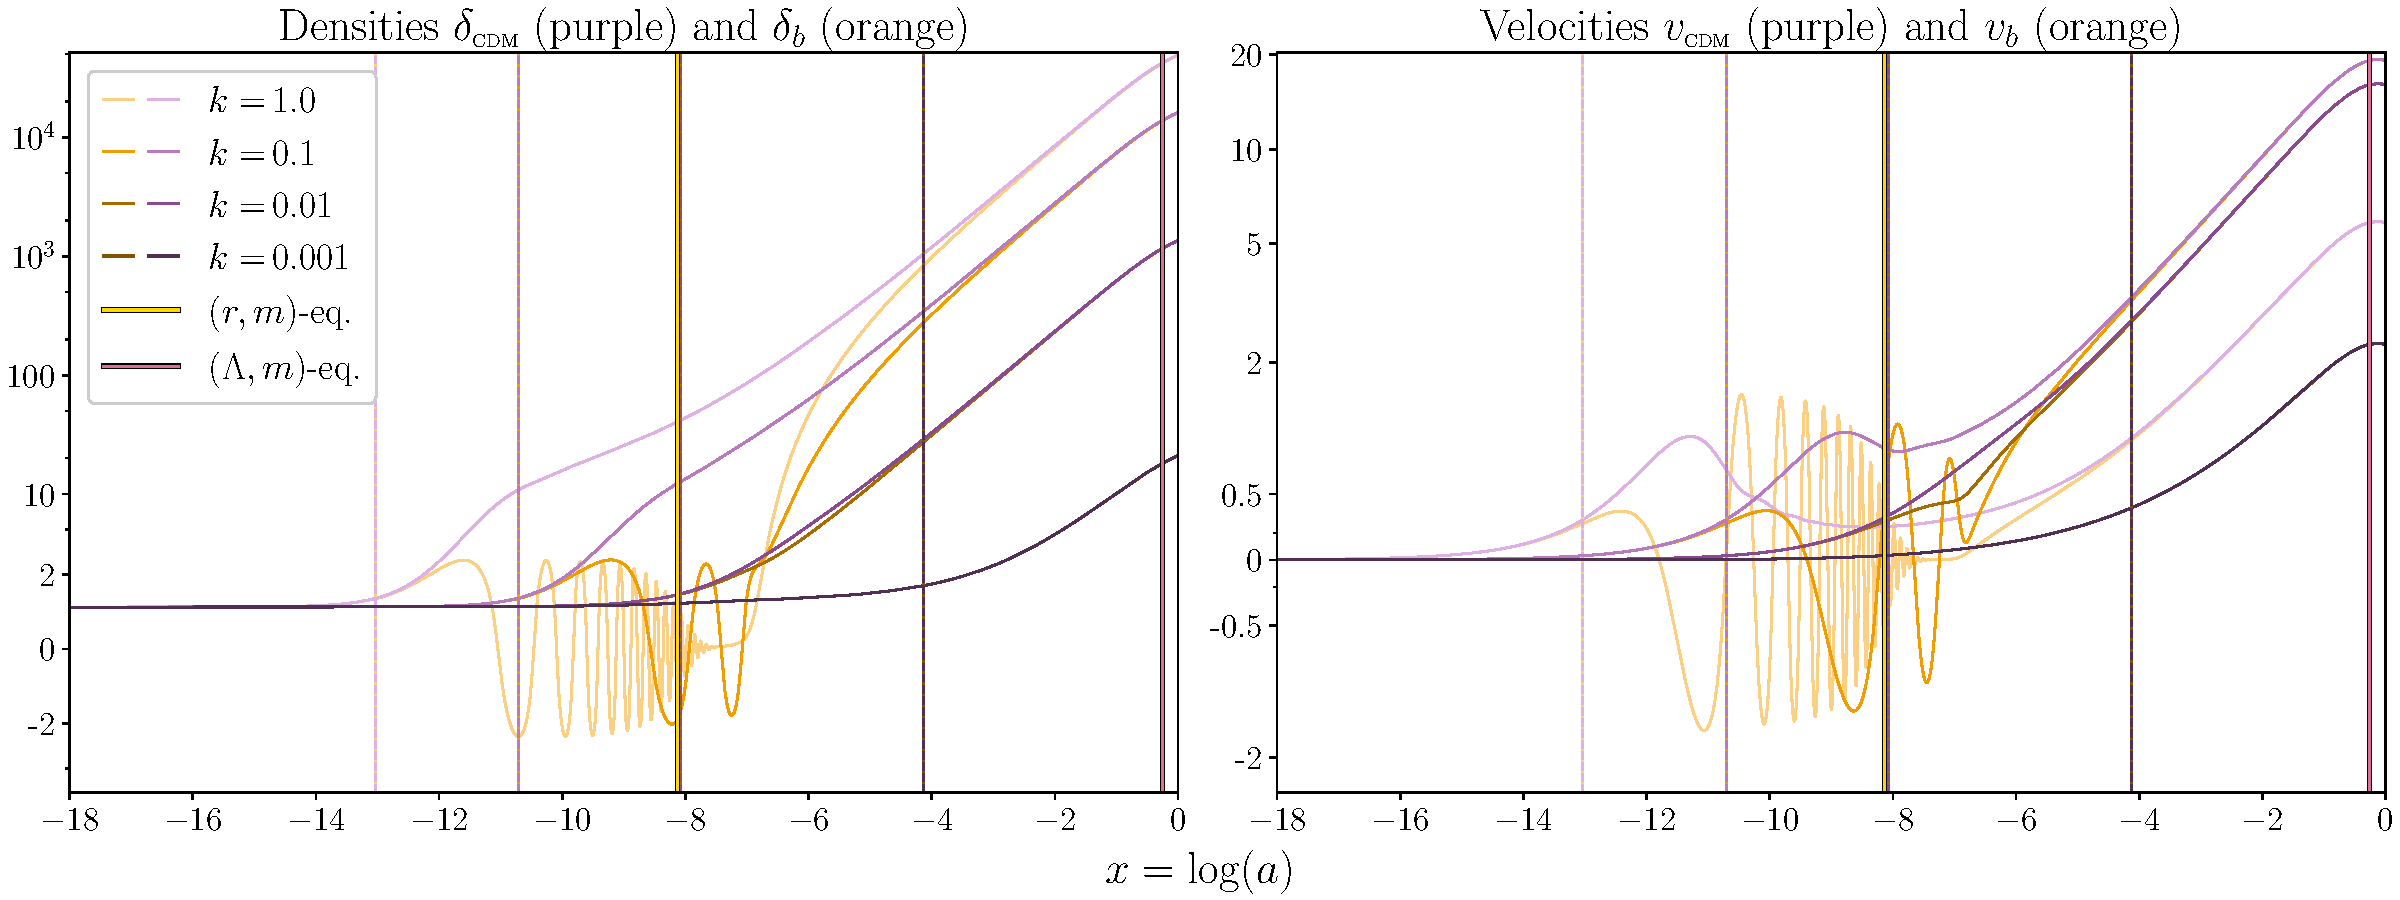
\includegraphics[width=\textwidth]{/Users/paljettrosa/Documents/GitHub/AST5220/figs/CDM_and_baryons.pdf}
  \caption{Evolution of the CDM (purple shades) and baryon (orange shades) density (left) and velocity (right) perturbations. Darker lines correspond to larger scales (smaller $k$, given in units of $\text{Mpc}^{-1}$). An asinh-scaling is used to highlight variations across several orders of magnitude and sign changes. Dashed lines indicate approximate horizon entry times for different modes, while the yellow and red vertical lines mark radiation-matter and matter-dark energy equality, respectively. \colorbox{Plum}{should I explain the asinh scaling?}}\label{fig:CDM and baryons}
\end{figure*}

Figure \ref{fig:CDM and baryons} shows the evolution of the density contrasts $\delta_\text{CDM}$ and $\delta_b$ (left panel) and the corresponding velocity perturbations $v_\text{CDM}$ and $v_b$ (right panel), plotted as functions of $x = \log (a)$ for the four selected wavenumbers mentioned in section \ref{subsubsec: III methods limits}. Darker colors correspond to smaller $k$ (larger scales), and vertical dashed lines mark the approximate horizon entry for each mode, estimated by $ck/\mathcal{H} = 1$. \colorbox{Plum}{should I explain this?} The yellow and red lines indicate radiation-matter and matter-dark energy equality, respectively.

Small-scale modes ($k = 1.0$, $0.1\,\text{Mpc}^{-1}$) enter the horizon during radiation domination, when the energy density is dominated by relativistic species that cannot cluster efficiently. As a result, gravitational potentials decay, suppressing the growth of matter overdensities—a phenomenon known as the Meszaros effect. In this regime, CDM perturbations grow only logarithmically until matter domination sets in. This suppression is driven indirectly by radiation pressure, which causes the decay of gravitational wells and weakens the gravitational pull that would otherwise enhance CDM growth. Since dark matter does not couple directly to photons, this suppression is slightly delayed compared to baryons. CDM overdensities continue to grow briefly after horizon entry, with velocity perturbations peaking slightly later (e.g., around $x \sim -11.5$ for $k = 1.0\,\text{Mpc}^{-1}$), before growth eventually stalls.

For baryons, the behavior is markedly different prior to recombination. In addition to being affected by the decaying gravitational wells, they experience acoustic oscillations driven by photon pressure due to their tight coupling through Thomson scattering. This is visible in the velocity plot as rapid oscillations for the highest $k$-mode following horizon entry. The radiation pressure prevents effective baryon clustering, leading to oscillations in $\delta_b$ and preventing the growth observed in $\delta_\text{CDM}$. The onset of oscillations is slightly delayed by the gravitational pull from growing CDM overdensities, which initially drive the baryons into the same potential wells. However, the direct interaction with photons soon dominates, causing the velocity divergence to reverse and oscillate.

The intermediate mode ($k = 0.01\,\text{Mpc}^{-1}$), which enters the horizon around the time of radiation-matter equality, displays a hybrid behavior. Initially, its growth is mildly suppressed by residual radiation pressure, causing the baryon overdensity to lag slightly behind that of dark matter. After recombination, however, the diminishing influence of photon scattering allows baryons to fall freely into CDM potential wells. This leads to the observed  convergence of the baryon and CDM perturbations, with any residual oscillations in the baryon velocity field decaying rapidly as pressure support fades. The largest mode ($k = 0.001\,\text{Mpc}^{-1}$) enters the horizon well after matter-radiation equality, and evolves in a regime where gravitational potentials are nearly constant. Consequently, both CDM and baryon overdensities grow roughly in proportion to the scale factor, with steadily increasing and closely aligned velocity perturbations, unaffected by oscillatory behavior.

At late times, after matter-dark energy equality (marked by the red line), the accelerated expansion caused by dark energy suppresses the growth of all matter perturbations. This is reflected in the flattening of the density contrast curves and the gradual decrease of velocity perturbations for all modes, and is the result of decaying of gravitational potentials. This leads to a freeze-out in structure formation, and is closely related to the ISW effect mentioned in section \ref{subsubsec: III theory photons}. 
% which leaves a significant imprint on the CMB power spectrum as we will see in the next milestone. \colorbox{Plum}{maybe rewrite/shorten}
% as discussed in secton \ref{subsubsec: III results Phi and Psi}. 


\subsubsection{Photons and neutrinos}

\begin{figure*}
  \centering
  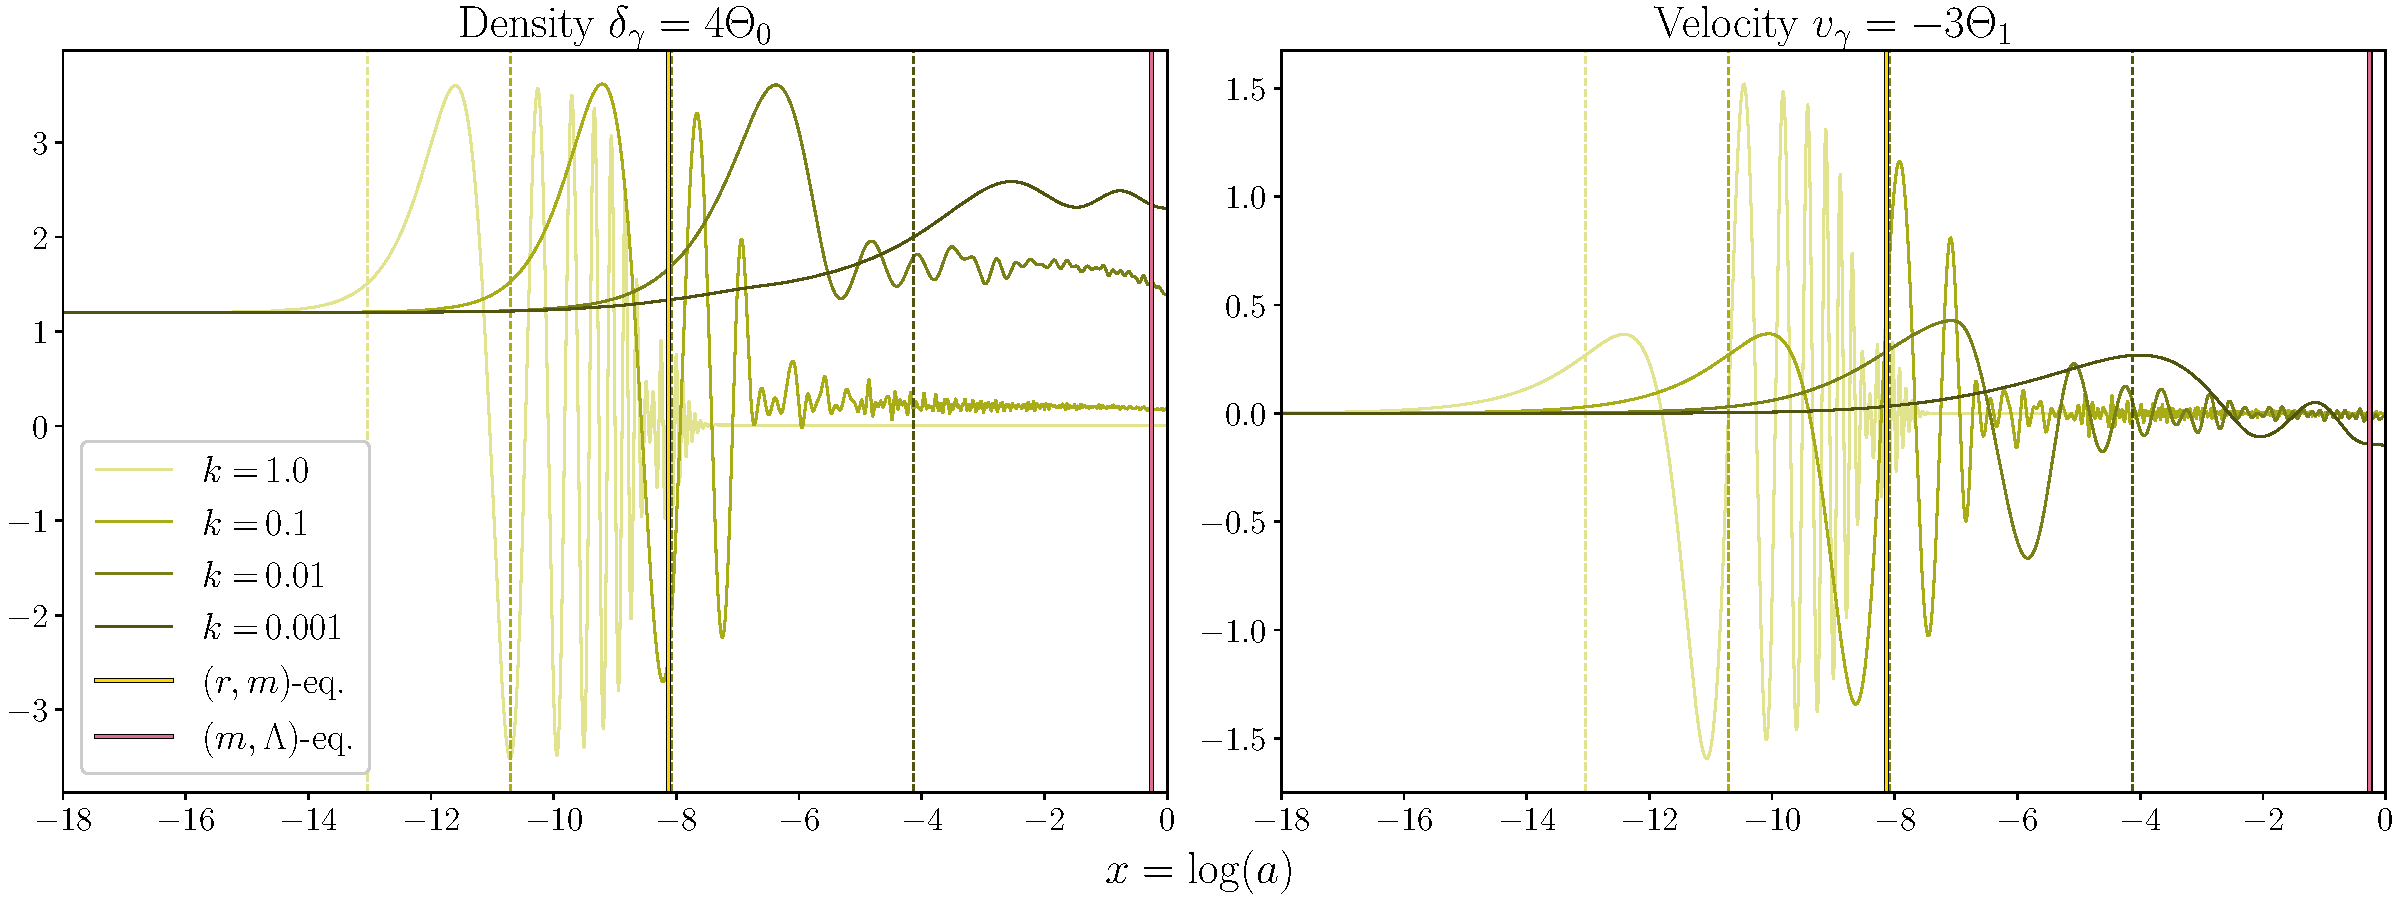
\includegraphics[width=\textwidth]{/Users/paljettrosa/Documents/GitHub/AST5220/figs/photons.pdf}
  \caption{Evolution of photon density $\delta_\gamma=4\Theta_0$ (left) and velocity $v_\gamma=-3\Theta_1$ (right) perturbations. 
  %Darker lines represent larger scales, and the $k$-values are given in units of $\text{Mpc}^{-1}$. 
  The photon perturbations grow and oscillate after horizon entry, with oscillations damping over time, especially for small-scale modes after matter-radiation equality.}\label{fig:photons}
\end{figure*}

Figure \ref{fig:photons} displays the evolution of the photon density perturbations $\delta_\gamma = 4\Theta_0$ (left panel) and velocity perturbations $v_\gamma = -3\Theta_1$ (right panel), for the same range of $k$-values as previously. Before horizon entry, all modes evolve slowly and remain nearly constant due to the absence of causal interactions. If a mode enters the horizon before or around the time of recombination, it begins to oscillate due to acoustic waves in the tightly coupled photon-baryon plasma, mimicking the behavior seen for baryons in figure \ref{fig:CDM and baryons}. These oscillations are governed by the interplay between gravitational compression and the restoring pressure of the photons, effectively behaving like a driven harmonic oscillator.

For the modes that enter the horizon during radiation domination (e.g., $k=0.1$ and $1.0\,\text{Mpc}^{-1}$), oscillations begin early and with high frequency. However, their amplitude gradually decays over time due to diffusion damping (Silk damping), where photons scatter and diffuse out of overdense regions, erasing anisotropies on small scales. This leads to the observed rapid suppression of oscillations in both $\delta_\gamma$ and $v_\gamma$ for these high-$k$ modes after radiation-matter equality. In contrast, large-scale modes ($k=0.001$ and $0.01\,\text{Mpc}^{-1}$) enter the horizon later, during or after matter domination. As a result, they begin oscillating later and at lower frequencies, and their amplitudes are less affected by damping. 
% This results in more sustained and coherent oscillatory behavior. Notably, the $k=0.01\,\text{Mpc}^{-1}$ mode maintains significant amplitude well into the matter-dominated era, reflecting continued gravitational driving before damping dominates.

The velocity perturbations $v_\gamma$ track the same oscillation frequency as $\delta_\gamma$, but are phase-shifted by $\pi/2$, consistent with harmonic oscillator dynamics. Their amplitudes evolve similarly, decreasing with time due to the same damping mechanisms, with small-scale modes decaying more rapidly than large-scale ones. Their sign reflects the direction of bulk photon motion associated with compressions and rarefactions in the fluid.


\begin{figure*}
  \centering
  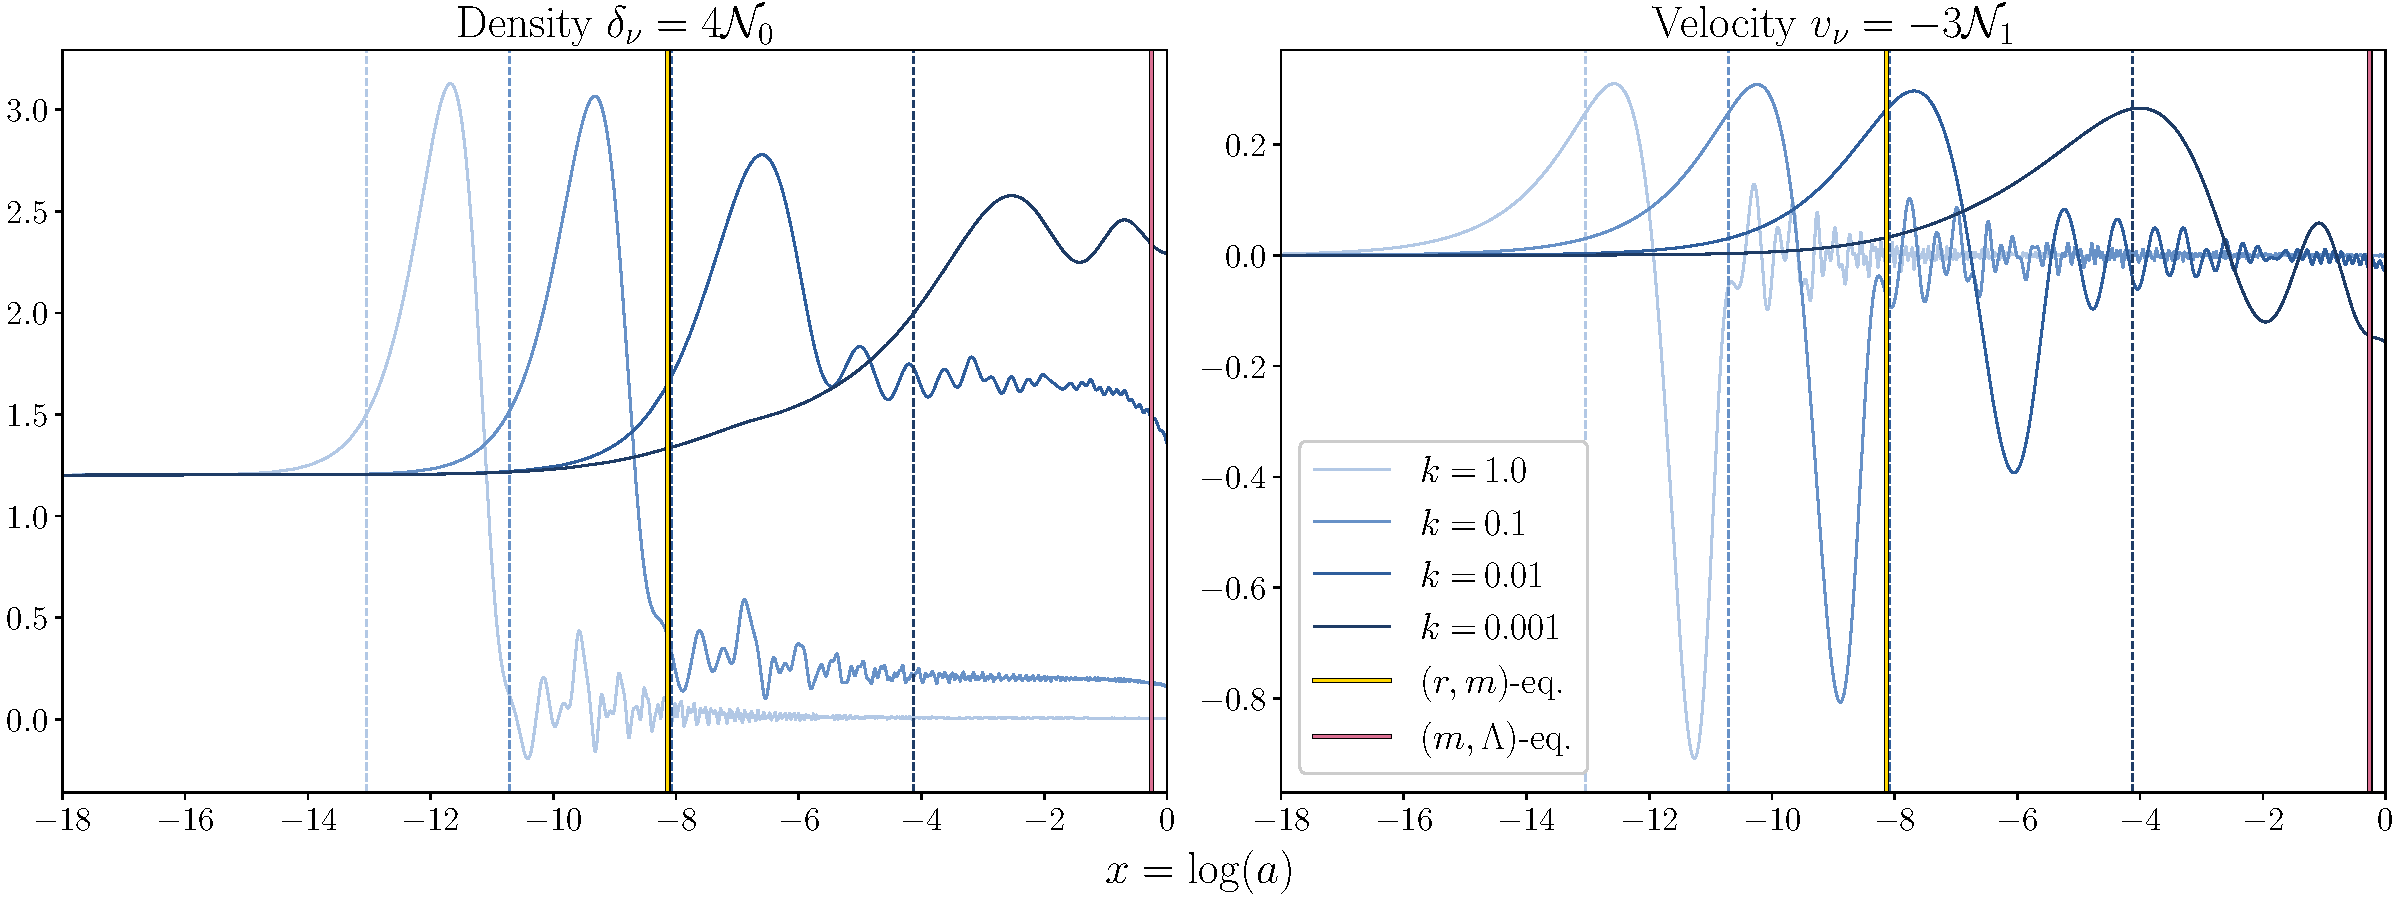
\includegraphics[width=\textwidth]{/Users/paljettrosa/Documents/GitHub/AST5220/figs/neutrinos.pdf}
  \caption{Evolution of neutrino density $\delta_\nu=4\mathcal{N}_0$ (left) and velocity $v_\nu=-3\mathcal{N}_1$ (right) perturbations. 
  %Darker lines show larger scales, with $k$-values stated in $\text{Mpc}^{-1}$ as before. \colorbox{Plum}{necessary to state every time?} 
  Neutrino perturbations behave similarly to photons at early times but evolve differently due to free-streaming, with scale-dependent residuals emerging after horizon entry.}\label{fig:neutrinos}
\end{figure*}

Figure \ref{fig:neutrinos} shows the evolution of the neutrino density contrast $\delta_\nu = 4\mathcal{N}_0$ (left) and velocity perturbation $v_\nu = -3\mathcal{N}_1$ (right) for the same range of wavenumbers. Before horizon entry, all perturbations evolve slowly and remain nearly constant, consistent with the causal limitations imposed on superhorizon modes.

Unlike photons, neutrinos decoupled at temperatures around $1\,$MeV and have been free-streaming ever since. As a result, their perturbations evolve collisionlessly, and begin to oscillate immediately after horizon crossing. However, because neutrinos do not participate in the tight-coupling dynamics of the photon-baryon fluid, they are not subject to the same restoring forces, and their perturbations are not sustained by acoustic oscillations. Consequently, we see that the velocity and density contrasts in neutrinos decay more rapidly than their photon counterparts. This damping is particularly strong for small-scale modes, where the free-streaming is most effective at erasing inhomogeneities.
% unlike the sustained oscillations seen in photons, neutrino perturbations are quickly damped due to the rapid dispersion of neutrinos in momentum space. This damping is particularly strong for small-scale modes, where the free-streaming is most effective at erasing inhomogeneities.

At late times, the accelerated expansion driven by dark energy suppresses the growth of all perturbations. For relativistic species like photons and neutrinos, whose energy densities dilute more rapidly with expansion ($\rho_r \propto a^{-4}$), this results in a gradual decline in their density contrasts. This behavior is evident in the intermediate-scale modes shown in figures \ref{fig:photons} and \ref{fig:neutrinos}, where the perturbations—following an extended period of near-constant oscillations—begin to decay as we approach matter-dark energy equality.

% The different asymptotic values of $\delta_\nu$ for the various $k$-modes can be understood from the balance between gravitational driving and free-streaming. Larger-scale modes are affected by gravitational potentials for a longer time before horizon entry and can retain more of their initial amplitude, whereas small-scale modes are rapidly damped by free-streaming once they enter the horizon. This explains the downward trend in $\delta_\nu$ for increasing $k$ in the late-time Universe.


\subsubsection{Quadrupole moments}\label{subsubsec: III results quadrupoles}

\begin{figure*}
  \centering
  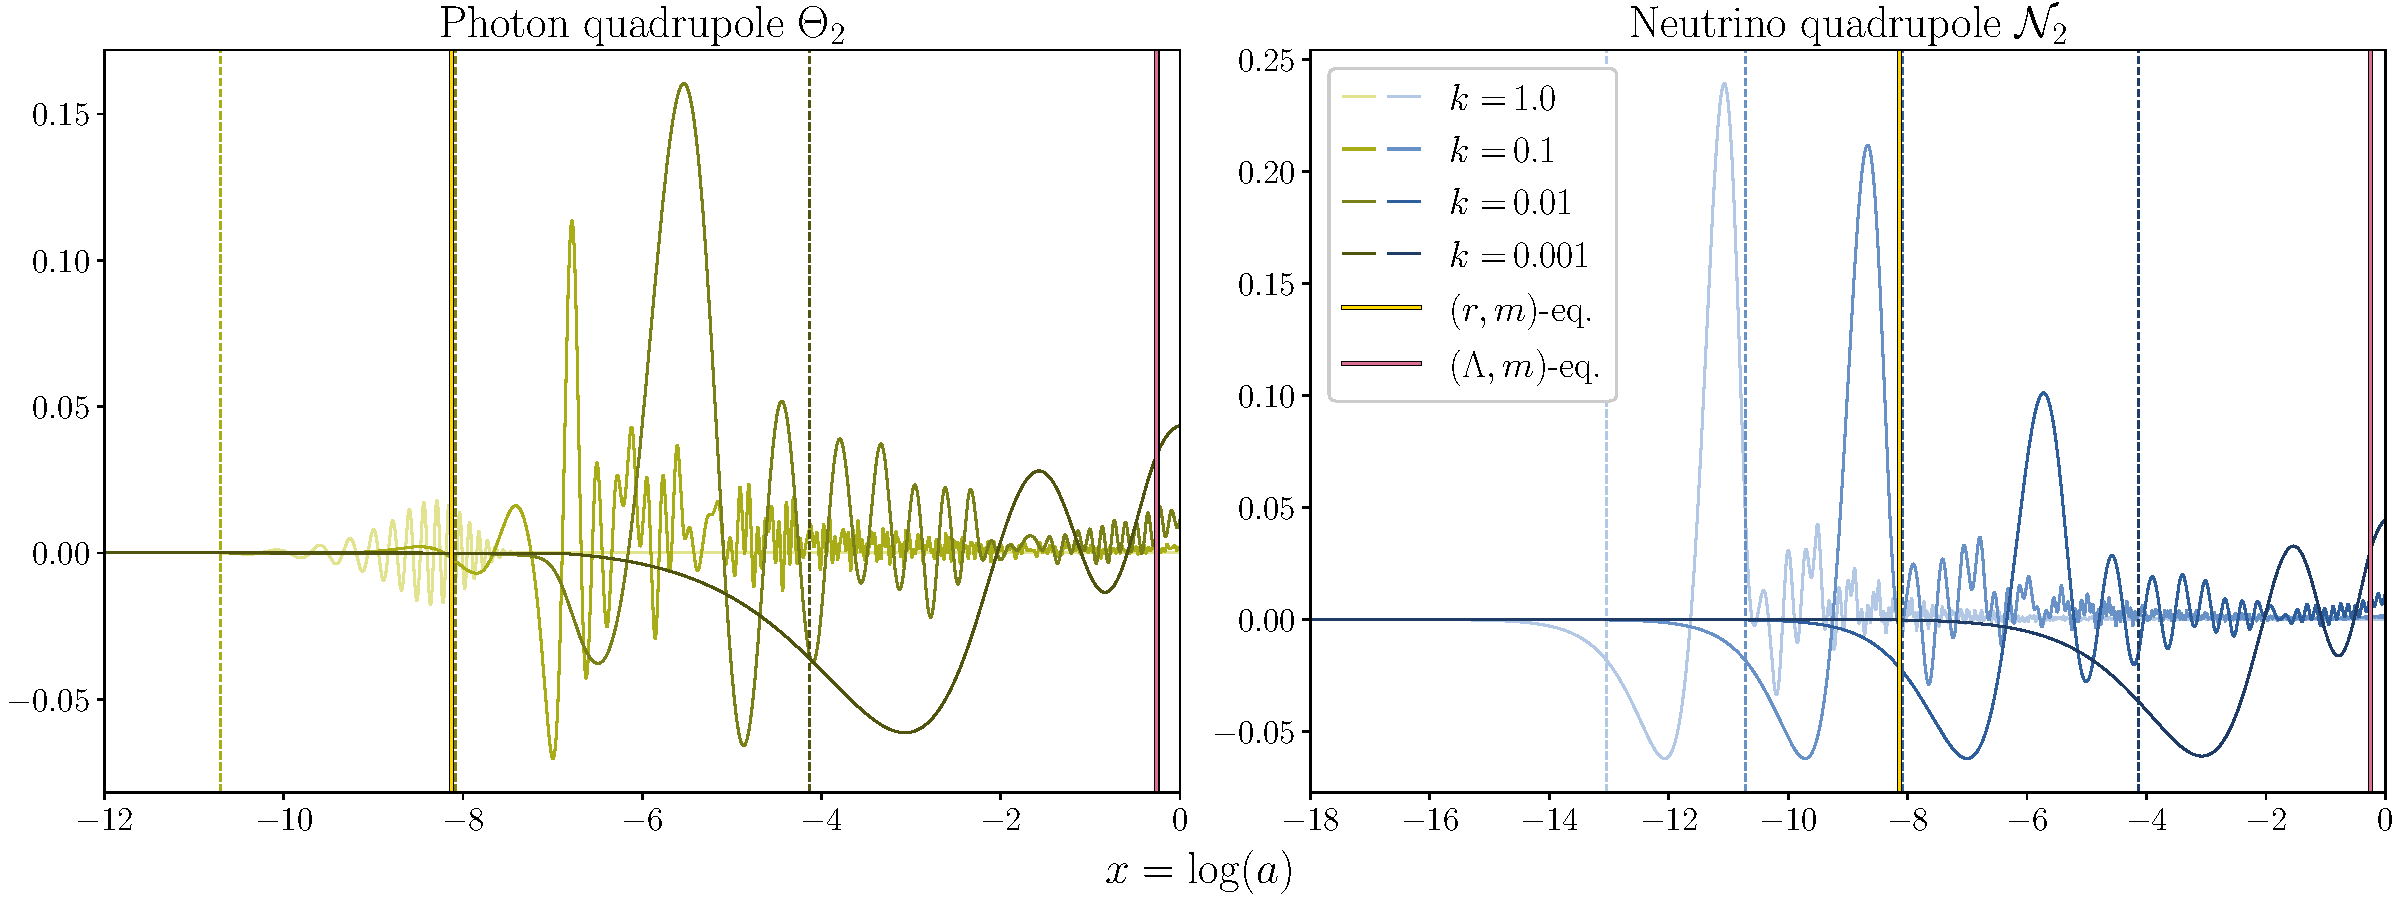
\includegraphics[width=\textwidth]{/Users/paljettrosa/Documents/GitHub/AST5220/figs/quadrupoles.pdf}
  \caption{Evolution of the photon quadrupole $\Theta_2$ (left) and the neutrino quadrupole $\mathcal{N}_2$ (right). 
  %Darker curves correspond to larger scales, and $k$ is given in units of $\text{Mpc}^{-1}$. 
  The photon quadrupole remains suppressed until tight-coupling breaks down, while the neutrino quadrupole freely grows after horizon crossing.}\label{fig:quadrupoles}
\end{figure*}

Figure \ref{fig:quadrupoles} shows the evolution of the photon (left) and neutrino (right) quadrupoles. In the left panel, the $x$-axis is cropped to exclude most of the tight-coupling era, during which $\Theta_2$ is heavily suppressed due to rapid Thomson scattering. After tight-coupling breaks down near recombination, a non-zero photon quadrupole rapidly develops, though its evolution varies strongly with scale. For the largest $k$-mode, $\Theta_2$ begins oscillating shortly after horizon entry and is quickly damped by residual scattering and diffusion. In contrast, the second largest mode exhibits more pronounced and irregular oscillations that persist further into the matter-dominated era before gradually decaying—highlighting the continued interplay between acoustic driving and damping processes described earlier.

The second smallest $k$-mode exhibits the most pronounced and sustained oscillations. Although the amplitude gradually decays following recombination, a significant growth is observable around $x \sim -2$, coinciding with the onset of reionization. This timing might suggest that renewed Thomson scattering off free electrons reintroduced during reionization may allow for temporary amplification of the quadrupole through new anisotropic photon scattering. \colorbox{Plum}{is this reasonable?}

Turning to $\mathcal{N}_2$, we observe a visibly different pattern, especially on small scales. Due to the very early neutrino decoupling, their quadrupole begins growing immediately after horizon entry for each mode, unimpeded by scattering. The smaller-scale modes peak at higher amplitudes due to more efficient free-streaming and earlier entry into the horizon, while the large-scale modes enter later and thus remain nearly flat until matter domination. In the radiation-dominated era, neutrinos contribute significantly to the anisotropic stress. Since they can develop a quadrupole immediately upon horizon entry, they also play an important role in the decay of the gravitational potential $\Phi$ on subhorizon scales.

A noteworthy late-time feature is the gentle upward trend in both $\Theta_2$ and $\mathcal{N}_2$ for the large- and intermediate-scale modes after matter-dark energy equality. This can be attributed to the decay of gravitational potentials in the dark energy-dominated era, which acts as a source for anisotropies via the ISW effect. The fact that this trend appears in both the photon and neutrino quadrupoles suggests it is unlikely to be a consequence of reionization, as neutrinos are unaffected by scattering processes.

\color{Plum}
QUESTION: Could the increase towards $x=0$ be a numerical artifact caused by including too many multipoles? Or does it actually have a physical significance? It disappears if I reduce to 8 multipoles of each type. I'm honestly guessing a little here, because I think it's kinda difficult to interpret.
\color{black}


\subsubsection{Polarization multipoles}

\begin{figure}
  \centering
  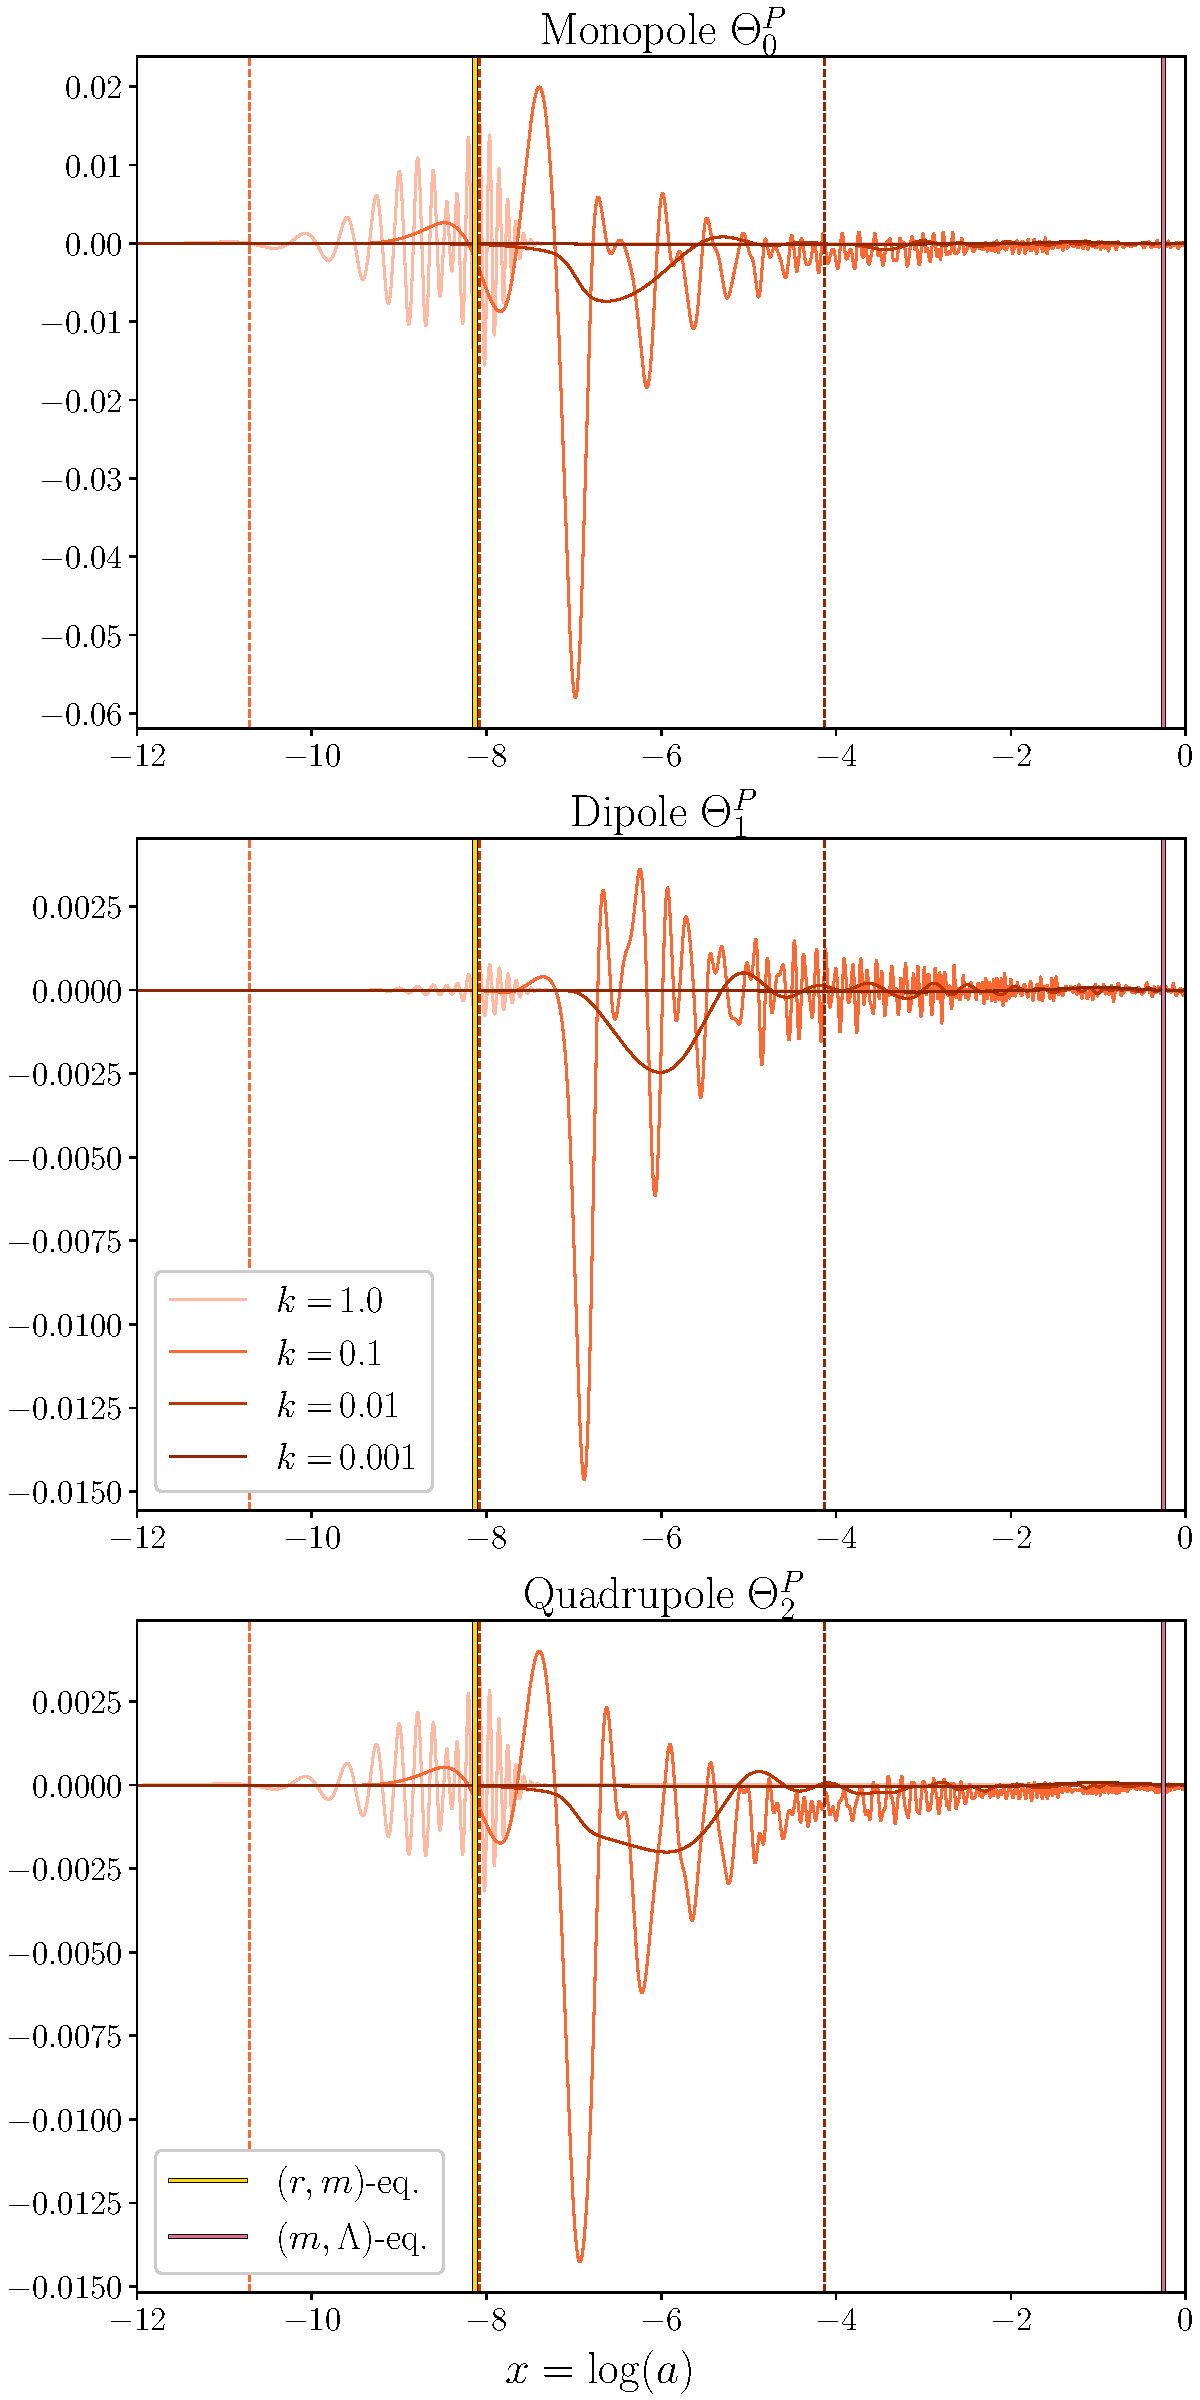
\includegraphics[width=\columnwidth]{/Users/paljettrosa/Documents/GitHub/AST5220/figs/polarization.pdf}
  \caption{Evolution of the polarization monopole $\Theta^P_0$ (top), dipole $\Theta^P_1$ (middle), and quadrupole $\Theta^P_2$ (bottom). Polarization arises from the temperature quadrupole anisotropy, becoming significant only after tight-coupling ends.}\label{fig:polarization}
\end{figure}


Figure \ref{fig:polarization} shows the evolution of the photon polarization monopole $\Theta^P_{0}$ (top panel), dipole $\Theta^P_{1}$ (middle panel), and quadrupole $\Theta^P_{2}$ (bottom panel). In contrast to photon temperature perturbations, all the polarization multipoles are sourced by the anisotropic Thomson scattering that becomes effective only after photon decoupling. Consequently, they are vanishingly small in the early Universe, and the $x$-axis is cropped in the plot to highlight their relevant evolution.

The smallest-scale mode, which enters the horizon deep in the radiation era, naturally begins oscillating first. Its polarization multipoles closely track the oscillatory pattern of $\Theta_2$ from figure \ref{fig:quadrupoles}, consistent with the fact that all polarization multipoles are algebraically related to the temperature quadrupole in the tight-coupling regime. Their oscillations also persist with decreasing amplitude after radiation-matter equality, echoing the damping seen for $\Theta_2$.

The intermediate-scale modes show more irregular oscillatory behavior, with noticeable shifts and non-monotonic amplitudes. This may be partially influenced by reionization at $x \gtrsim -2$, which reintroduces Thomson scattering and allows the quadrupole to again source polarization. Interestingly, $\Theta^P_{0}$ and $\Theta^P_{2}$ for these modes appear to be consistently shifted slightly below zero, suggesting a net anisotropic distortion in one direction due to residual quadrupole contributions or asymmetric reionization effects. \colorbox{Plum}{or possibly a numerical artifact?}

Finally, the largest-scale mode exhibits almost no oscillation in any of the polarization multipoles, despite the quadrupole $\Theta_2$ for this mode showing clear growth after horizon entry. This mismatch is a consequence of the limited causal interaction at such large scales: the polarization generation is inefficient due to the lack of significant Thomson scattering at late times and therefore insufficient anisotropy build-up.



\subsubsection{Gravitational potentials}\label{subsubsec: III results Phi and Psi}

\begin{figure*}
  \centering
  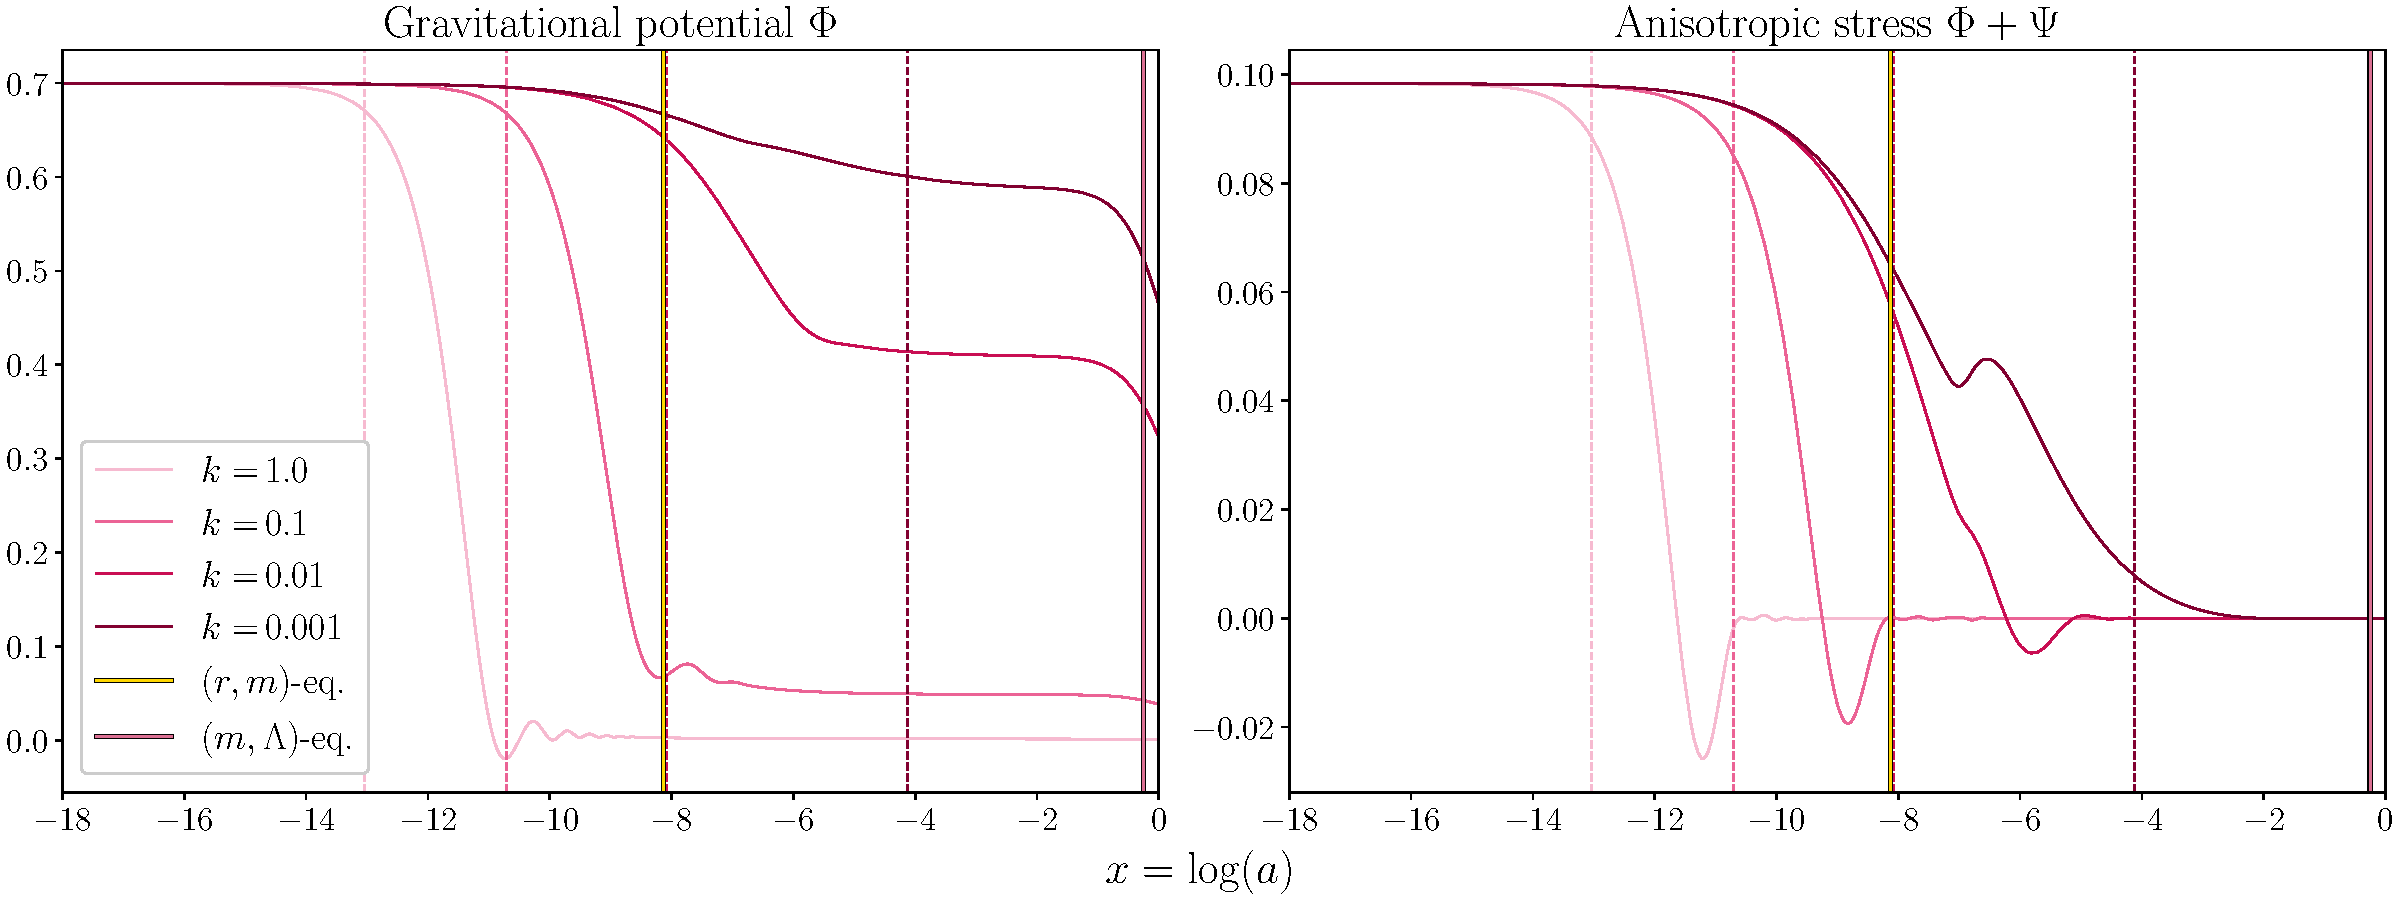
\includegraphics[width=\textwidth]{/Users/paljettrosa/Documents/GitHub/AST5220/figs/Phi_and_Psi.pdf}
  \caption{Evolution of the gravitational potential $\Phi$ (left) and the anisotropic stress $\Phi + \Psi$ (right). 
  %Darker lines show larger scales, with $k$-values stated in $\text{Mpc}^{-1}$ as before. 
  Small-scale modes that enter the horizon during radiation domination exhibit decaying $\Phi$ and oscillatory $\Phi + \Psi$, while large-scale modes preserve nearly constant potentials until dark energy domination.
  % as functions of $x = \log (a)$. Darker lines correspond to larger scales (smaller $k$, given in units of $\text{Mpc}^{-1}$). Dashed lines indicate approximate horizon entry times for different modes, while the yellow and red vertical lines mark radiation-matter and matter-dark energy equality, respectively.
  }\label{fig:Phi and Psi}
\end{figure*}

Figure \ref{fig:Phi and Psi} shows the evolution of the gravitational potential $\Phi$ (left) and the anisotropic stress $\Phi + \Psi$ (right). During radiation domination, $\Phi$ remains nearly constant for superhorizon modes, consistent with the conservation of the comoving curvature perturbation $\mathcal{R}$. In contrast, for the smallest-scale modes that enter the horizon during this epoch, $\Phi$ decays rapidly. This occurs because the dominating radiation pressure prevents the sustain of stable gravitational potential wells and inhibits efficient matter clustering. As illustrated in figures \ref{fig:CDM and baryons} and \ref{fig:photons}, this decay contributes both to the onset of acoustic oscillations in the photon-baryon fluid and to the suppressed growth of CDM overdensities via the Meszaros effect.

The intermediate mode $k = 0.01\,\text{Mpc}^{-1}$ enters the horizon around the time of radiation-matter equality, and its behavior reflects the transition between these two regimes. Its gravitational potential exhibits a modest decay while radiation still contributes significantly to the total energy density, but soon flattens as CDM begins to dominate and support stable potential wells. This pattern aligns with the sustained growth of matter perturbations seen for this mode and helps explain its prolonged oscillatory behavior in the photon and neutrino quadrupole plots (figure \ref{fig:quadrupoles}).

For the largest scale, which enters well after matter domination, $\Phi$ remains nearly constant after horizon entry. Here, CDM clustering is fully efficient, and the lack of significant radiation pressure means potential wells remain effectively static. This reflects the standard Meszaros transition, where structure formation proceeds unimpeded by relativistic species. At late times, however, all modes exhibit a decline in $\Phi$ as dark energy becomes dominant. As mentioned briefly in the previous sections, this decay of potentials contributes to the late-time ISW effect, which sources large-scale temperature anisotropies in the CMB.

The right panel of figure \ref{fig:Phi and Psi} illustrates how the anisotropic stress $\Phi + \Psi$ evolves across different scales and epochs. For high-$k$ modes entering the horizon during radiation domination, we observe a rapid decline from the initial positive value, followed by oscillations around zero with a decaying amplitude. This pattern reflects the onset of anisotropic stress caused by free-streaming neutrinos. As seen in figure \ref{fig:quadrupoles}, the neutrino quadrupole $\mathcal{N}_2$ grows rapidly once a mode enters the horizon, generating anisotropic stress that alters the Einstein equations by suppressing $\Psi$ relative to $\Phi$ (see eq. \eqref{eq: Psi}). This in turn causes $\Phi + \Psi$ to deviate from its initial value and oscillate.

These oscillations also affect the evolution of $\Phi$, as both $\Psi$ and the neutrino quadrupole $\mathcal{N}_2$ enter its differential equation (eq. \eqref{eq: dPhidx}). On small scales, this coupling drives the rapid decay of the gravitational potentials. As the Universe transitions to matter domination, the impact of free-streaming relativistic species weakens, leading to a gradual decline in anisotropic stress. For the intermediate mode ($k = 0.01\,\text{Mpc}^{-1}$), this change appears as a brief dip in $\Phi + \Psi$ just after horizon entry, followed by a steady return toward zero, reflecting the residual but diminishing influence of radiation. In contrast, the largest-scale mode exhibits only a modest positive bump before smoothly flattening out. In both cases, $\Phi + \Psi$ approaches zero at late times, consistent with a pressureless fluid in which anisotropic stress vanishes and $\Phi = -\Psi$.

\color{Plum}
QUESTION: Is it okay to have this subsection at the end? I placed it here because I wanted to refer to the quadrupole plots when discussing the anisotropic stress, but I don't know if these things should be presented earlier.
\color{black}





% \subsubsection{Density perturbations}
% \begin{figure*}
%   \centering
%   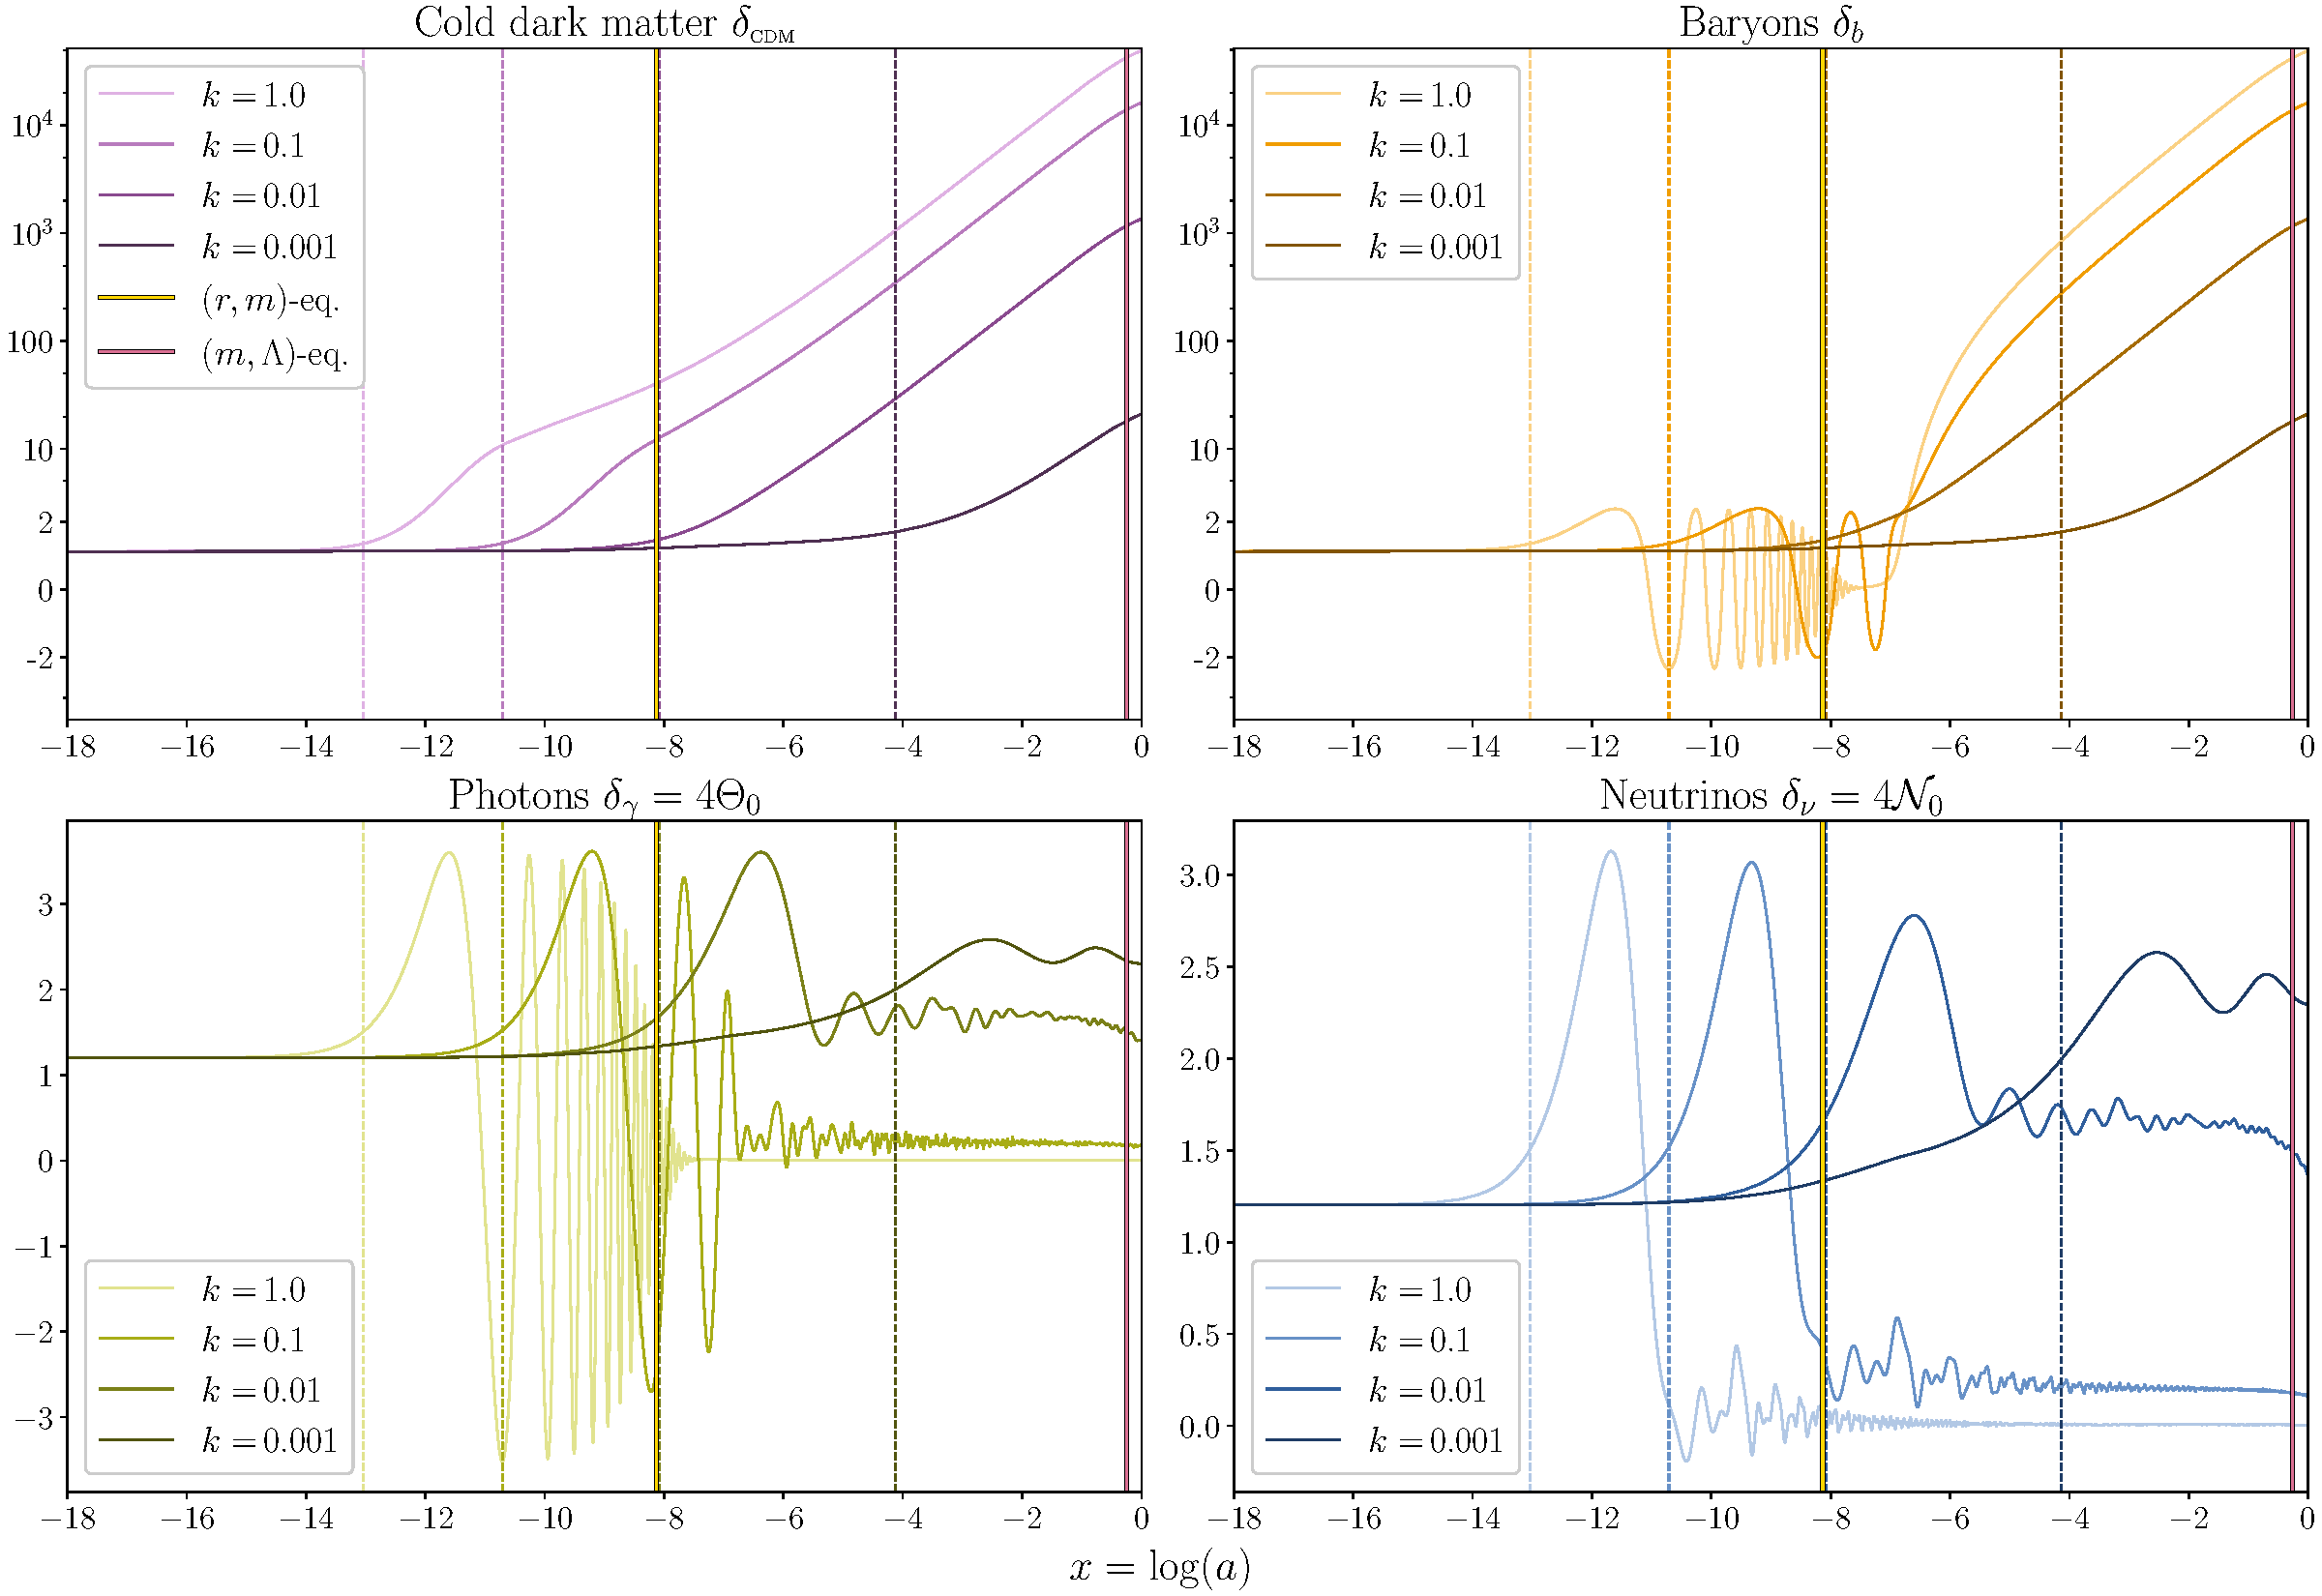
\includegraphics[width=\textwidth]{/Users/paljettrosa/Documents/GitHub/AST5220/figs/densities.pdf}
%   \caption{Evolution of the CDM (top left), baryon (top right), photon (bottom left) and neutrino (bottom right) overdensities. Darker lines correspond to larger scales (smaller $k$, given in units of $\text{Mpc}^{-1}$). The CDM and baryon plots use an asinh-scale to highlight variations across several orders of magnitude and sign changes. Dashed lines indicate approximate horizon entry times for different modes, while the yellow and red vertical lines mark radiation-matter and matter-dark energy equality, respectively. \colorbox{Plum}{TODO: maybe change, explain asinh?}}\label{fig:densities}
% \end{figure*}

% \color{Plum}
% Figure \ref{fig:densities} shows the evolution of the density contrasts $\delta_i$ for cold dark matter (top left), baryons (top right), photons (bottom left), and neutrinos (bottom right) as functions of $x = \log (a)$ for the four selected wavenumbers mentioned in section \ref{subsubsec: III methods limits}. Darker curves correspond to larger spatial scales (smaller $k$), and the dashed vertical lines mark the approximate horizon entry times for each mode, estimated by the condition $ck/\mathcal{H} = 1$. \colorbox{Plum}{should I explain this?} The yellow and red vertical lines indicate radiation-matter and matter-dark energy equality, respectively.

% In the top two panels, we see that CDM and baryons share similar growth behavior on large scales, as well as on smaller scales before horizon entry and well after after recombination. Prior to horizon entry, all matter perturbations grow slowly due to causal constraints. After entering the horizon, modes that do so during radiation domination (e.g. $k = 1.0$ and $0.1$ Mpc$^{-1}$) experience suppressed growth—a manifestation of the Meszaros effect. Here, radiation dominates the energy density and gravitational potentials decay, inhibiting efficient structure formation. These modes continue to grow only logarithmically until matter takes over, but not before the corresponding velocity contrasts have sufficiently decayed due to the rapid radiation-driven expansion. This is visible from 

% By contrast, modes that enter the horizon after matter-radiation equality (e.g. $k = 0.001$ Mpc$^{-1}$) grow more efficiently upon horizon entry, as cold dark matter can now dominate and maintain gravitational potential wells. As expected, the largest-scale CDM perturbations reach the highest amplitudes by today. The intermediate mode ($k = 0.01$ Mpc$^{-1}$), which enters around equality, displays a transition between the two regimes, with some early suppression followed by linear growth—highlighting the gradual nature of equality.

% Baryons closely follow the photon field before recombination due to tight coupling. As a result, $\delta_b$ exhibits oscillatory behavior prior to decoupling. After recombination, baryons decouple from photons and begin falling into CDM potential wells, causing $\delta_b$ to converge toward $\delta_\text{CDM}$. The convergence is slower for smaller-scale modes due to lingering pressure support and photon drag.

% The bottom panels illustrate photon and neutrino density perturbations. Both species are relativistic and free-streaming after their respective decoupling epochs. After horizon entry, both $\delta_\gamma$ and $\delta_\nu$ undergo oscillations, though their behavior differs. Photons oscillate in the coupled photon-baryon fluid, forming acoustic waves with decaying amplitude due to Silk damping. Neutrinos, having decoupled much earlier, evolve collisionlessly and undergo free-streaming, which causes more rapid damping and smoothed perturbations. This distinction becomes evident at high $k$.

% Unlike photons, neutrinos are unaffected by recombination, so their oscillations continue undisturbed until matter domination, after which their contribution becomes subdominant. Notably, $\delta_\nu$ settles at different asymptotic values for different $k$ due to the competing effects of free-streaming and gravitational driving prior to horizon entry.

% Together, these panels highlight how different species respond to horizon crossing, coupling mechanisms, and the dominant energy component of the Universe. These density perturbations in turn source gravitational potentials and drive the evolution of velocity perturbations, which we discuss in the following subsection.
% \color{black}


% \subsubsection{Velocity perturbations}
% \begin{figure*}
%   \centering
%   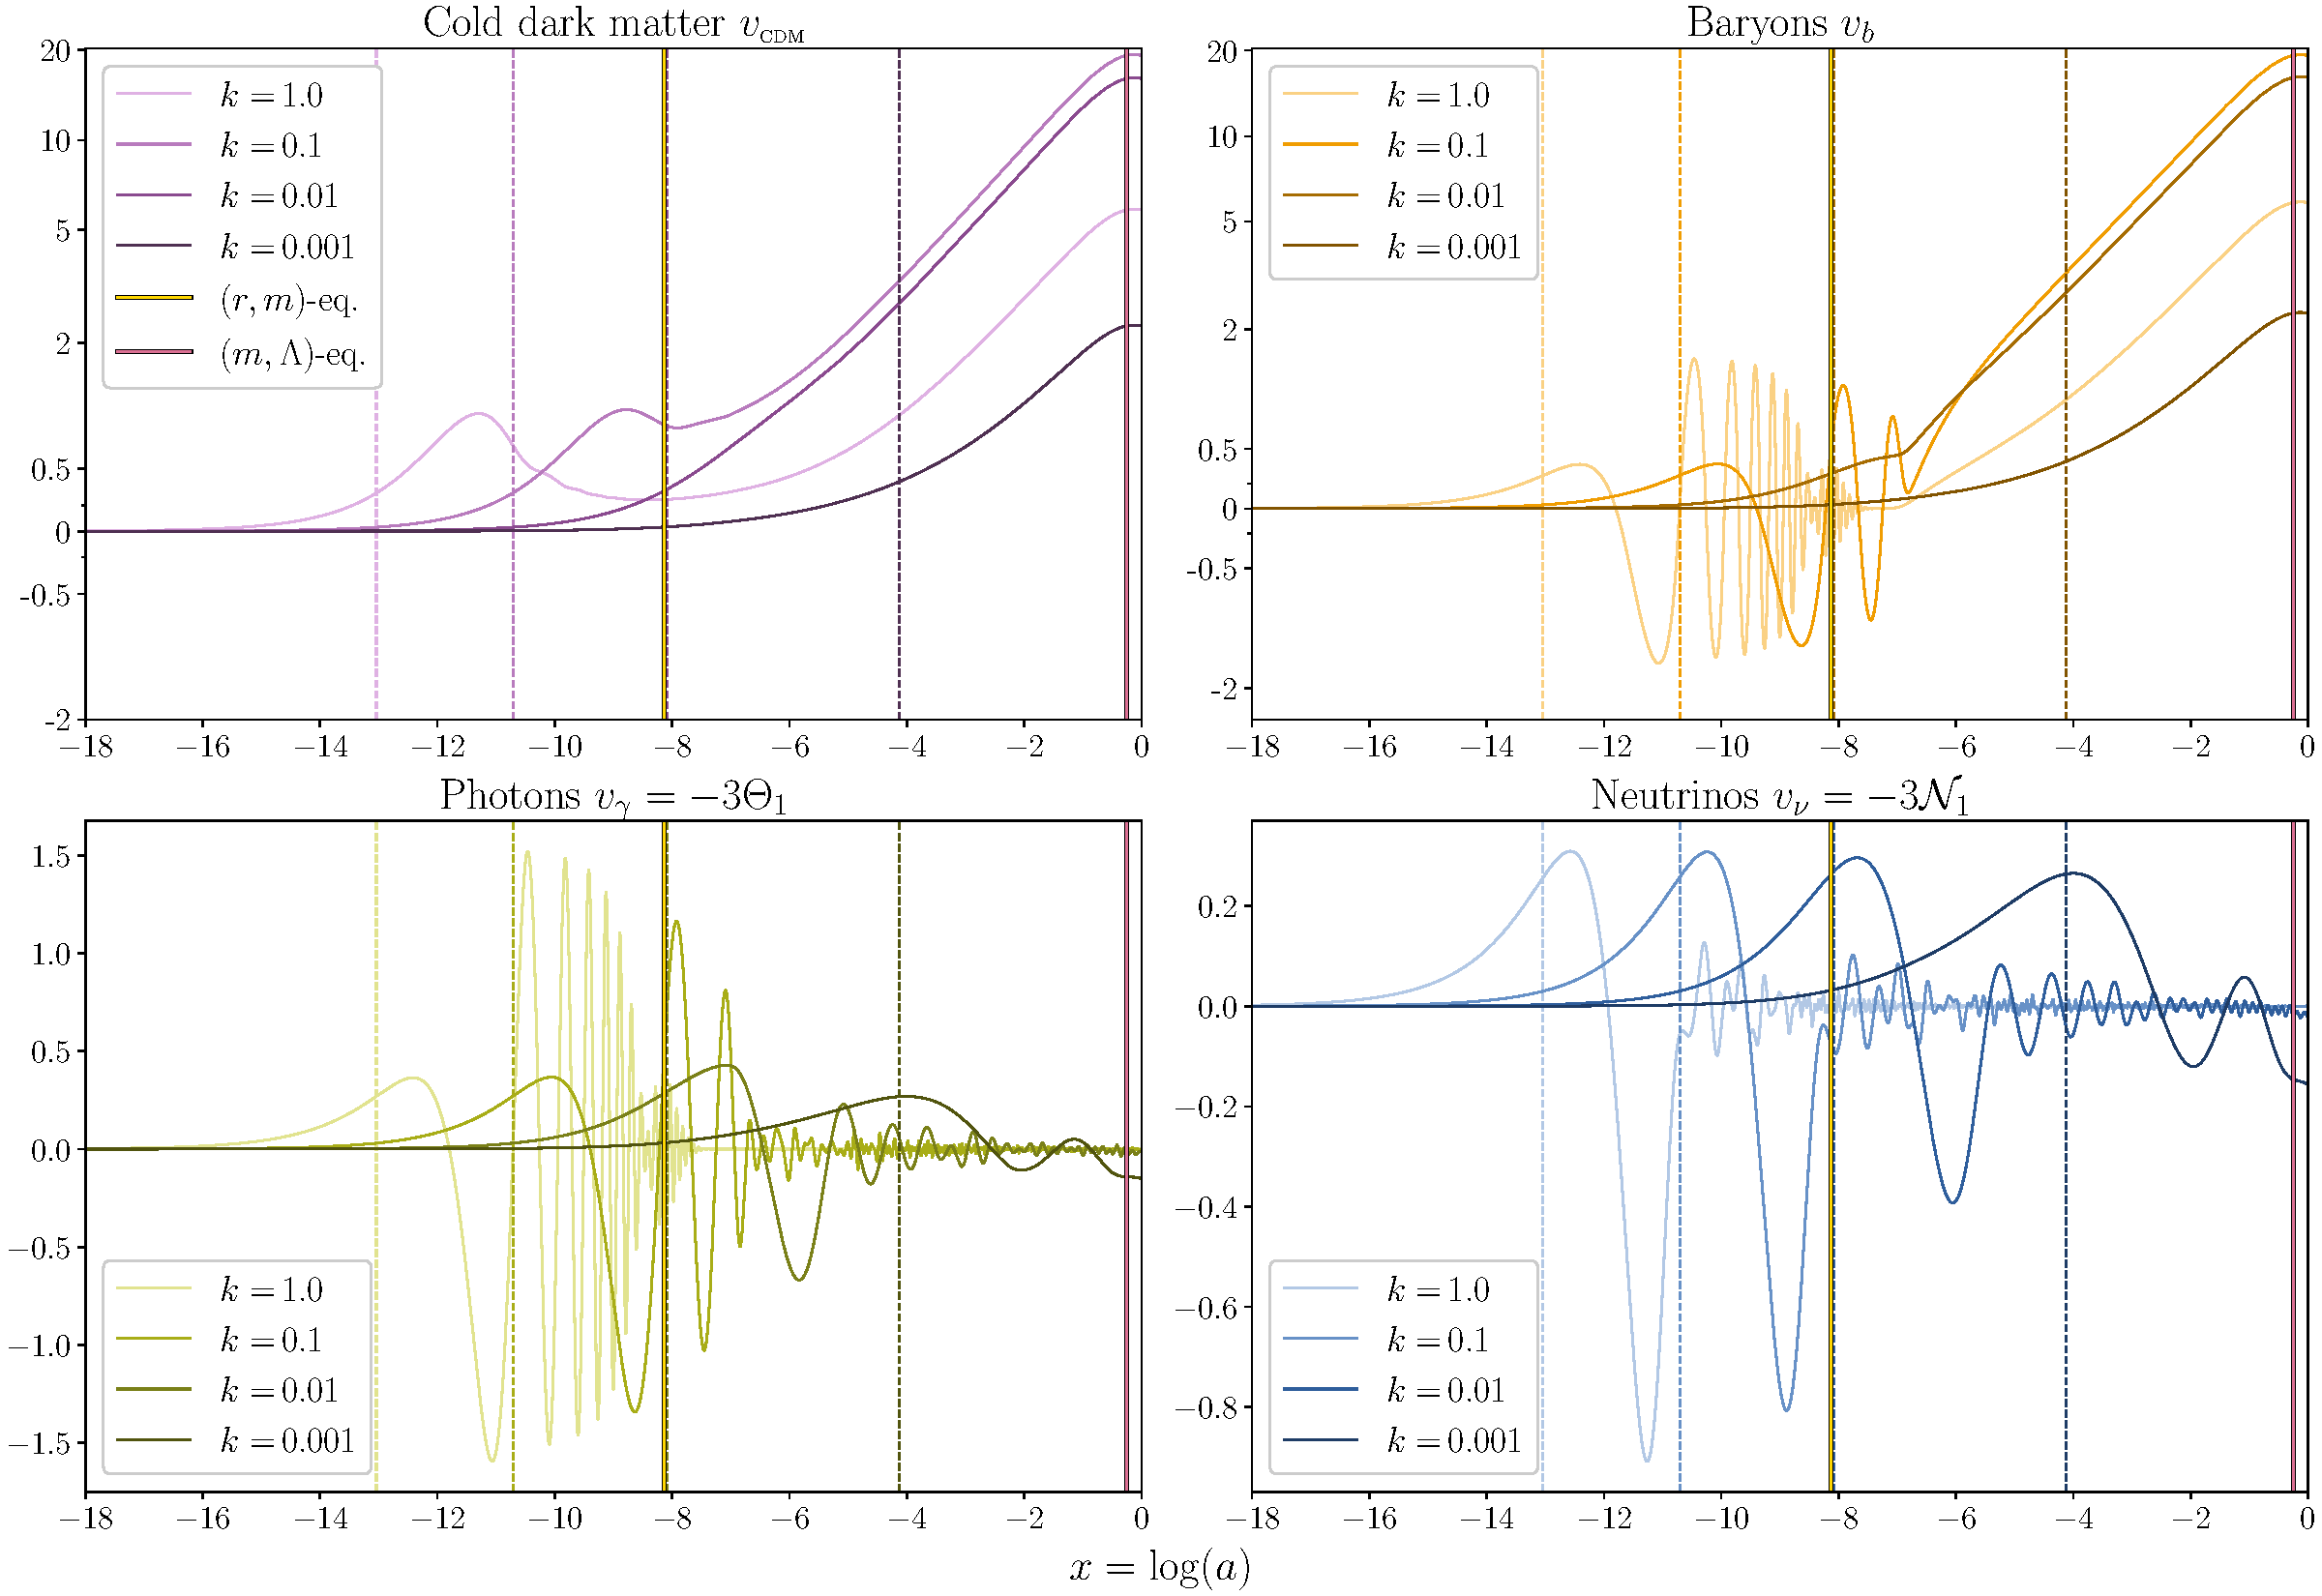
\includegraphics[width=\textwidth]{/Users/paljettrosa/Documents/GitHub/AST5220/figs/velocities.pdf}
%   \caption{Evolution of the CDM (upper left), baryon (upper right), photon (lower left) and neutrino (lower right) velocity perturbations. Darker lines indicate larger scales, and the values of $k$ are in units of $\text{Mpc}^{-1}$. The CDM and baryon plots use an asinh-scale to highlight variations across several orders of magnitude and sign changes. Key cosmological transitions are indicated as in the previous figure.}\label{fig:velocities}
% \end{figure*}

% \color{Plum}
% Figure \ref{fig:velocities} displays the evolution of the velocity perturbations $v_i$ for cold dark matter (CDM), baryons, photons, and neutrinos. Each subplot shows $v_i$ as a function of $x = \log(a)$ for four representative wavenumbers $k = 0.001$, $0.01$, $0.1$, and $1.0,\text{Mpc}^{-1}$, with darker curves corresponding to larger spatial scales (smaller $k$). Vertical yellow and red lines denote radiation-matter equality and matter-dark energy equality, respectively.

% Before horizon entry, all velocities remain close to zero due to the superhorizon nature of the perturbations—causal processes have not yet begun to operate. Upon horizon entry, each component begins to develop velocity perturbations, responding to gravitational potentials and pressure forces.

% For CDM, which is pressureless and uncoupled from other species, the velocity perturbations increase monotonically after horizon entry and eventually freeze out during dark energy domination. This behavior reflects CDM's smooth infall into growing gravitational potentials, with no oscillatory motion due to the absence of pressure.

% In contrast, baryon velocities initially track those of photons closely, displaying clear acoustic oscillations for high-$k$ modes. This behavior arises from the tight coupling between baryons and photons before recombination, where the photon pressure drives oscillations in the combined photon-baryon fluid. The amplitude and frequency of these oscillations are determined by the sound speed of the fluid and the wavenumber. After recombination, photons decouple and begin free-streaming, allowing baryons to fall more freely into gravitational wells. As a result, the baryon velocities start to align with the CDM velocities, and oscillations gradually damp out.

% Photon and neutrino velocity perturbations also exhibit oscillatory behavior following horizon entry. For photons, the oscillations stem from the harmonic response of the tightly coupled photon-baryon fluid to gravitational compression and rarefaction. These oscillations are phase-shifted by $\pi/2$ relative to the density fluctuations, consistent with the harmonic oscillator model described in Milestone III. The amplitude of $v_\gamma$ decreases after matter-radiation equality due to Silk damping, which erases small-scale perturbations via photon diffusion.

% Neutrinos, which decoupled early and have been free-streaming ever since, display qualitatively similar oscillations to photons but with key differences. Unlike photons, they are not subject to tight coupling or Silk damping, and thus their velocity perturbations exhibit broader oscillations with less damping. Nevertheless, the free-streaming nature of neutrinos causes their perturbations to spread out in phase space, leading to an overall suppression of small-scale modes after horizon entry.

% Comparing all components, we see that photon and baryon velocities are initially synchronized due to tight coupling, while CDM and neutrinos evolve independently. The eventual alignment of baryon and CDM velocities after recombination reflects the transition to baryons behaving like a pressureless fluid. The distinct evolution of photon and neutrino velocities also highlights the impact of interactions (or lack thereof) on perturbation growth, which in turn affects the gravitational potentials that drive structure formation. These insights set the stage for the next subsections on higher-order multipoles and the evolution of $\Phi$ and $\Psi$.
% \color{black}











\section{Milestone IV: Power Spectra}\label{sec: milestone IV}
Having explored the background evolution of the Universe, its thermal history, and the growth of perturbations, we now reach the final step: computing the primary statistical observables in cosmology—the CMB power spectrum and the matter power spectrum. These spectra encode the evolution of perturbations from their initial conditions to their imprint on the cosmic microwave background and the large-scale distribution of matter. Their precise computation allows us to compare theoretical predictions with observations from missions such as Planck, placing stringent constraints on cosmological parameters.  

The CMB power spectrum quantifies temperature and polarization anisotropies in the CMB sky, which arise from acoustic oscillations in the early Universe, gravitational redshifting, and scattering effects. To compute this spectrum, we must perform line-of-sight integration, tracing how photons have propagated from recombination to today, incorporating contributions from Sachs-Wolfe effects, Doppler shifts, and polarization terms. The matter power spectrum, on the other hand, describes how density fluctuations in the Universe are distributed across different scales today. It is derived from the total matter perturbations, including contributions from dark matter and baryons, and plays a crucial role in understanding the formation of large-scale structure.  

By synthesizing the physics from all previous milestones, this milestone brings us to the final stage of our Einstein-Boltzmann solver. The results will allow direct comparison with observational data, testing the validity of our theoretical model and its numerical implementation.

\colorbox{Plum}{TODO: shorten/word different to fit the rest}




\subsection{Theoretical framework}\label{subsec: IV theory}
% \begin{enumerate}
%   \item [1.] Explain how we can write the photon temperature field in terms of spherical harmonics, and define what these are.
%   \item [2.] Explain why the CMB power spectrum is the square of the coefficients in the spherical harmonics expansion, and explain what the $\ell$'s and $m$'s mean. Explain also explicitly why there is no $m$-dependence, and we therefore write $C_\ell$.
%   \item [3.] Explain thoroughly what the line-of-sight integration method is, who developed it, how it works and why it works.
%   \item [4.] Explain and derive explicitly what the source function is, and explain that this comes from the milestone III result. Explain what each term means, where they come from and how they affect the power spectrum.
%   \item [5.] Explain what the spherical bessel functions are, and why we use these when we perform line-of-sight integration (take into account the projection of the 3D characterized by $k$ onto a 2D sphere characterized by $\ell$).
%   \item [6.] Explain how we can use the spline of the photon temperature and polarization multipoles to obtain the CMB power spectra for temperature and polarization, repsectively. Explain also the differences between the TT, TE and EE maps.
%   \item [7.] Write explicitly the general expression for the primordial power spectrum, and explain where it comes from.
%   \item [8.] Explain that most inflation models predict a so-called Harrison-Zel'dovich primordial spectrum, and explicitly write out the form of this. 
%   \item [9.] Explain what cosmic variance is, state the expression for it and explain how it will inevitably affect the results.
%   \item [10.] Explain how we can generate a CMB map with the help of the theoretical $C_\ell$ spectrum.
%   \item [11.] Explain how we compute the neutrino power spectrum, and why it is similar to the CMB spectrm. Write explicitly out the source function.
%   \item [12.] Explain what the matter power spectrum represents, and state the general expression for it. 
%   \item [13.] Explain what the gauge invariant matter density field is, and why we need it.
%   \item [14.] Explain how we can look at the matter power spectrum for individual components and state the general expression for $\Delta_i(k,x)$. Explain the terms.
%   \item [15.] Explain what the correlation function is (Fourier transform of the matter power-spectrum), and what it represents. Explain how we easily can compute it. Motivate that it is interesting to study because of baryon acoustic oscillations?
%   \item [16.] Explain what the angular correlation function is, and state the expression from the problem description appendix.
%   \item [17.] Explain how we can compute the effects of gravitational lensing on the CMB temperature power spectrum, and write explicitly the expression for the lensed correlation function. Also write explicitly what $\sigma^2(\theta)$, $C_\text{gl}(\theta)$ and $C_\text{gl,2}(\theta)$ are, and what they physically represent. Also write out the expression for the reduced Wigner functions $d_{mn}^\ell(\theta)$. 
%   \item [18.] Explain why the effects of gravitational lensing are interesting, and how we expect it to affect the power spectrum.
% \end{enumerate}
% Points 1 and 2 are for subsection 1 (temperature fluctuations as spherical harmonics), points 3-5 for subsection 2 (line-of-sight integration), points 6-10 for subsection 3 (the CMB power spectra), point 11 for subsection 4 (the neutrino power spectrum), points 12-14 for subsection 5 (the matter power spectrum), point 15 for subsection 6 (the correlation function), and points 16-18 for subsection 7 (effects of gravitational lensing).


% Can you write subsection 7 about the effects of gravitational lensing? Make sure to include points 16-18: 
% \item [16.] Explain what the angular correlation function is, and state the expression from the problem description appendix.
% \item [17.] Explain how we can compute the effects of gravitational lensing on the CMB temperature power spectrum, and write explicitly the expression for the lensed correlation function. Also write explicitly what $\sigma^2(\theta)$, $C_\text{gl}(\theta)$ and $C_\text{gl,2}(\theta)$ are, and what they physically represent. Also write out the expression for the reduced Wigner functions $d_{mn}^\ell(\theta)$. 
% \item [18.] Explain why the effects of gravitational lensing are interesting, and how we expect it to affect the power spectrum.

\subsubsection{Temperature fluctuations as spherical harmonics}
To begin understanding the CMB power spectrum, we must connect our theoretical results to the actual observable: the temperature fluctuations of the CMB across the sky. These are quantified by the temperature field $\Theta(t,\vec{x},\hat{p})$ introduced in the previous milestone, which we already know how to solve for in Fourier space. 
% These are measured as small deviations from the average temperature $T(\hat{n})$ in different directions $\hat{n}$. After subtracting the mean temperature, the relative fluctuation is defined as  
% \begin{equation}
% \frac{\delta T}{T} = \Theta(t,\vec{x}, \hat{p}),
% \end{equation}
% where $\Theta$ is the photon temperature perturbation we solved for, $\hat{p}$ is the line-of-sight direction, and $t$ is the time of observation, typically taken as today. 
Since the sky is a two-dimensional sphere, it is natural to expand this temperature field in terms of spherical harmonics:  
\begin{equation}
\Theta(t, \vec{x}, \hat{p}) = \sum_{\ell=1}^{\infty} \sum_{m=-\ell}^{\ell} a_{\ell m}(t, \vec{x}) Y_{\ell m}(\hat{p}).
\end{equation}
Here, $Y_{\ell m}$ are the spherical harmonic functions that form a complete basis on the sphere, and the coefficients $a_{\ell m}$ describe the amplitude of fluctuations at angular scale $\ell$ and azimuthal mode $m$. By expressing $\Theta$ in terms of its Fourier components we can compute these coefficients as
\begin{equation}
  a_{\ell m}(t,\vec{x}) = \int\frac{d^3k}{2\pi^3}e^{i\vec{k}\cdot\vec{x}}\int Y^*_{\ell m}(\hat{p})\Theta(t,\vec{k},\hat{p})\,d\Omega_{\hat{p}}. \label{eq: coeffs}
\end{equation}
\colorbox{Plum}{TODO: remove? rewrite to fit 4.17 and 4.18?}

The multipole index $\ell$ is inversely related to the angular scale: low $\ell$ values correspond to large angular scales (broad patterns on the sky), while high $\ell$ values probe finer angular features. The $m$ index corresponds to different orientations of the pattern at a fixed angular scale. However, since the Universe is assumed to be statistically isotropic, the ensemble average of the temperature field must be invariant under rotations. This implies that there should be no preferred direction on the sky, and hence no statistical dependence on $m$. Consequently, we define the angular power spectrum as the variance of $a_{\ell m}$ over $m$:  
\begin{equation}
C_\ell \equiv \langle |a_{\ell m}|^2 \rangle = \frac{1}{2\ell+1} \sum_{m=-\ell}^{\ell} |a_{\ell m}|^2.
\end{equation}
Thus, the CMB power spectrum $C_\ell$ provides the average amplitude of temperature fluctuations as a function of angular scale $\ell$, and is the primary quantity we compare to observations. \\ \colorbox{Plum}{redundant?}

% To quantify the strength of temperature fluctuations at each angular scale, we define the CMB power spectrum as:
% \begin{equation}
% C_\ell = \langle |a_{\ell m}|^2 \rangle.
% \end{equation}
% This measures the variance of the spherical harmonic coefficients over different realizations of the universe. In an isotropic universe, there is no preferred direction, so the expectation value is independent of $m$, leading to:
% \begin{equation}
% C_\ell = \frac{1}{2\ell+1} \sum_{m=-\ell}^{\ell} |a_{\ell m}|^2.
% \end{equation}
% This result follows from the statistical isotropy of the CMB, which ensures that all $m$-modes for a given $\ell$ contain equal power on average.  
% \colorbox{Plum}{choose paragraph!}

A crucial point to emphasize is that we only observe one realization of the Universe. Theoretically, the average $\langle \cdot \rangle$ is meant to be an ensemble average over many universes with the same statistical properties. In practice, we must replace this ensemble average with an average over the $2\ell + 1$ available $m$-modes at each $\ell$, assuming ergodicity. 
% \colorbox{Plum}{TODO: maybe remove} 
This leads to a fundamental statistical limitation called cosmic variance. Since there are fewer $m$-modes at low $\ell$, our estimate of $C_\ell$ becomes increasingly uncertain on large angular scales. The cosmic variance is quantified by  
\begin{equation}
\frac{\mathrm{Var}(C_\ell)}{C_\ell^2} = \frac{2}{2\ell + 1},
\end{equation}
which shows that the relative uncertainty is larger for small $\ell$. Importantly, this is not a limitation of our instruments or data analysis, but a fundamental property of observing only one sky. As $\ell \to 0$, the number of independent modes becomes too small to robustly determine $C_\ell$, leading to large uncertainties in the low-$\ell$ regime of the power spectrum.








\subsubsection{Line-of-sight integration}\label{subsubsec: IV theory LOS}
To calculate the CMB angular power spectrum $C_\ell$, we need the temperature multipoles $\Theta_\ell(k)$ at present time. A naive approach would be to evolve the full Boltzmann hierarchy for each $\ell$ up to some large $\ell_{\text{max}} \sim 1000$, which would involve solving thousands of coupled differential equations for every mode $k$. While this is theoretically feasible, it is extremely computationally expensive. Fortunately, a clever method known as line-of-sight (LOS) integration (see \colorbox{Plum}{add citation!}) offers an elegant and much more efficient alternative.
% This technique was introduced by Uros Seljak and Matias Zaldarriaga in 1996 in their influential paper ``A Line of Sight Approach to Cosmic Microwave Background Anisotropies'' \colorbox{Plum}{add cite!}. 
Rather than evolving the entire Boltzmann hierarchy, this method instead solves for the monopole at all times and positions and then integrates over the photon path to determine the final anisotropies observed today. This drastically reduces the computational cost, requiring us to compute only a handful of lower multipoles, as mentioned in the previous milestone.
% \colorbox{Plum}{TODO: word different?}

At the heart of the LOS approach lies the so-called source function, which captures all physical effects that contribute to the temperature anisotropies observed in the CMB. It is derived by formally integrating the photon temperature perturbation equation from the last milestone, and isolating the directional dependence through integration by parts and multipole expansion. The final expression for the temperature multipole at present time $x = 0$ is:
\begin{equation}
\Theta_\ell(k, x=0) = \int_{-\infty}^{0} \tilde{S}(k, x) j_\ell\big[k(\eta_0 - \eta)\big]\, dx \label{eq: multipoles LOS}
\end{equation}
Here, $\tilde{S}(k, x)$ is the source function, and $j_\ell$ are spherical Bessel functions. Their appearance in the integral arises from the projection of three-dimensional spatial perturbations (characterized by wavevector magnitude $k$) onto the two-dimensional sky (characterized by angular multipole moment $\ell$). These functions emerge naturally when decomposing the plane wave $e^{i \vec{k} \cdot \vec{x}}$ into spherical harmonics and radial functions, and encode how fluctuations in a Fourier mode $k$ contribute to angular anisotropies at a given scale $\ell$. 
% \colorbox{Plum}{TODO: shorten?}
% Mathematically, this is captured by the expansion:
% \begin{equation}
% e^{i \vec{k} \cdot \vec{x}} = \sum_{\ell=0}^{\infty} (2\ell+1)i^\ell j_\ell(kx) P_\ell(\hat{k} \cdot \hat{x})
% \end{equation}
% Here, $j_\ell$ controls the radial dependence and determines the weight of a given $k$-mode in producing anisotropies at multipole $\ell$. These functions peak roughly when $k(\eta_0 - \eta) \sim \ell$, linking physical scale to angular scale on the sky.

One can show that the source function itself is given by:
\begin{align*}
\tilde{S}(k, x) =\, &\tilde{g} \left[ \Theta_0 + \Psi + \frac{1}{4} \Pi \right] + e^{-\tau} (\Psi' - \Phi') - \frac{1}{ck} \frac{d}{dx}(\mathcal{H} \tilde{g} v_b) \\
&+ \frac{3}{4 c^2 k^2} \frac{d}{dx} \left[ \mathcal{H} \frac{d}{dx} (\mathcal{H} \tilde{g} \Pi) \right], \numberthis
\end{align*}
Each term here has a specific physical interpretation: the first represents the monopole contribution (weighted by visibility), corrected by the gravitational redshift and polarization. Furthermore, $e^{-\tau}(\Psi' - \Phi')$ is simply the integrated Sachs-Wolfe (ISW) term, while the Doppler effect enters through the third term. The final term, involving $\Pi$, is a quadrupolar correction to the scattering due to anisotropic Thomson scattering, and includes polarization effects. In total, these terms encapsulate the full physics of how inhomogeneities in the early Universe source temperature anisotropies observed today. 
% \colorbox{Plum}{TODO: don't make redundant}
% The line-of-sight method allows us to compute $\Theta_\ell(k)$ efficiently via:
% \begin{equation}
% \Theta_\ell(k) = \int_{x_{\text{ini}}}^{0} dx\, \tilde{S}(k, x) j_\ell[k(\eta_0 - \eta(x))]
% \end{equation}
% This result combines the physics of recombination, gravitational redshifting, velocity effects, and polarization into a single, elegant expression. It drastically reduces the number of ODEs we need to solve and provides the foundation for computing the CMB power spectrum:
% \begin{equation}
% C_\ell = 4\pi \int_0^\infty A_s \left( \frac{k}{k_\text{pivot}} \right)^{n_s - 1} \Theta_\ell^2(k) \frac{dk}{k}
% \end{equation}
% This completes the core of the observable calculations in our Einstein-Boltzmann solver.





\subsubsection{Computing the temperature power spectrum}\label{subsubsec: IV theory CMB}
\colorbox{Plum}{rename section?}

Having computed the photon temperature multipoles $\Theta_\ell(k)$ through the line-of-sight integration method, we are in a position to extract one of the most important observables in modern cosmology: the angular CMB temperature power spectrum. 
% This spectrum, denoted $C_\ell$, encodes the variance of the temperature anisotropies as a function of angular scale on the sky. It provides a statistical summary of the CMB fluctuations and serves as a bridge between theoretical predictions and observational data.
% The theoretical angular power spectrum 
This is computed by first squaring the photon temperature multipoles obtained via the LOS method (eq. \eqref{eq: multipoles LOS}). We then multiply this with the primordial power spectrum mentioned in section \ref{subsubsec: III theory inflation} and integrate over all wave numbers $k$, which gives us:
\begin{equation}
    C_\ell = \frac{2}{\pi} \int k^2 P_\text{primordial}(k) \left| \Theta_\ell(k) \right|^2 \, dk. \label{eq: Cell1}
\end{equation}
Fortunately, most of the simplest single field inflation models predict a so-called Harrison-Zel'dovich spectrum:
\begin{equation}
  P_\text{primordial}(k) = \frac{2\pi^2}{k^3}\mathcal{P}_{\mathcal{R}}(k) = \frac{2\pi^2}{k^3}A_s \left( \frac{k}{k_\text{pivot}} \right)^{n_s - 1},
\end{equation}
where $A_s$ is the primordial amplitude, $n_s\sim1$ is the spectral index, and $k_\text{pivot}$ is a chosen reference scale. \colorbox{Plum}{explain origin?} Thus, using that the temperature multipoles $\Theta_\ell(k)$ must be real since they represent physical observables \colorbox{Plum}{correct?}, we may rewrite eq. \eqref{eq: Cell1} as
\begin{equation}
  C_\ell = 4\pi \int  A_s\left( \frac{k}{k_\text{pivot}} \right)^{n_s - 1} \Theta^2_\ell(k) \frac{dk}{k}, \label{eq: Cell2}
\end{equation}

% In addition to $C_\ell$, another quantity of interest is the angular correlation function of temperature fluctuations on the sky. It describes the expected correlation between temperature fluctuations at two points separated by an angle $\theta$, and is given by:
% \begin{equation}
%     C(\theta) = \sum_{\ell = 0}^{\infty} \frac{2\ell + 1}{4\pi} C_\ell P_\ell(\cos\theta),
% \end{equation}
% where $P_\ell$ are the Legendre polynomials. This function provides an intuitive real-space representation of how correlated the CMB is across different angular scales, and was historically used in early CMB analyses before the advent of full-sky harmonic transforms. \colorbox{black}{w/ lensing instead?}

Given the full theoretical $C_\ell$ spectrum, we can generate a synthetic realization of the CMB sky. This is interesting for comparing theory to actual observations, for visualizing the random nature of the CMB, and for generating mock data sets. However, to do this we must compute the coefficients $a_{\ell m}$ defined in eq. \eqref{eq: coeffs}.
% A full-sky map $T(\hat{n})$ of temperature fluctuations can be written as:
% \begin{equation}
%     T(\hat{n}) = \sum_{\ell m} a_{\ell m} Y_{\ell m}(\hat{n}),
% \end{equation}
% where the $a_{\ell m}$ coefficients are drawn from a Gaussian distribution with zero mean and variance given by $C_\ell$. Specifically, for each $(\ell, m)$:
% \begin{equation}
%     \langle a_{\ell m} a_{\ell' m'}^* \rangle = \delta_{\ell \ell'} \delta_{m m'} C_\ell.
% \end{equation}
A simple method for doing this is to sample them as complex Gaussian random variables with variance $C_\ell$, i.e.,
\begin{equation}
    a_{\ell m} = \sqrt{-\log (A) C_\ell} e^{2\pi i \theta},
\end{equation}
where $A$ and $\theta$ are random numbers drawn from a uniform distribution over $[0,1)$. To ensure that $T(\hat{n})$ is real-valued, we enforce:
\begin{equation}
    a_{\ell, -m} = (-1)^m a_{\ell m}^*.
\end{equation}
Once the $a_{\ell m}$'s are generated, the temperature map can be constructed using the HEALPIX library \colorbox{Plum}{add citation!}, which perform the spherical harmonic synthesis efficiently. 

\colorbox{Plum}{move/rewrite/specify in implementation?}


\subsubsection{Features in the CMB}\label{subsubsec: IV theory features}
\colorbox{Plum}{rename section? combine with previous?}

The prominent peaks and troughs observed in the power spectrum arise from acoustic oscillations in the tightly coupled photon-baryon fluid before recombination. These oscillations are the result of competition between gravitational collapse and photon pressure in the early Universe. Overdense regions begin to collapse under gravity, but the intense radiation pressure from photons resists compression, resulting in oscillatory behavior analogous to sound waves.

From figure \ref{fig:visibility function} presented in milestone II we know that the visibility function $\tilde{g}$ is sharply peaked around recombination. A rough approximation is thus $\tilde{g}\approx\delta(x-x_\text{rec})$, which according to eq. \eqref{eq: multipoles LOS} leads to
\begin{equation}
  \Theta^\text{today}_\ell(k) \approx \left[ \Theta_0+\Psi+\frac{\Pi}{4}\right]_\text{rec}\hspace{-6pt}j_\ell\big[k(\eta_0 - \eta_\text{rec})\big] \approx \left[ \Theta_0+\Psi\right]_\text{rec}\hspace{-1pt}j_\ell(k\eta_0).
\end{equation}
The second approximation follows from the fact that the anisotropy term is very small at recombination, and that $\eta_\text{rec}\ll\eta_0$. \colorbox{Plum}{word different?} Thus, we know that the dominant contribution to the observed anisotropies must come from the effective temperature perturbation at the time of recombination ($\left[ \Theta_0+\Psi\right]_\text{rec}$). 

To understand how this perturbation evolves, we may consider the coupled evolution equations for the monopole and dipole in terms of the conformal time:
\begin{align}
\frac{\partial \Theta_0}{\partial \eta} &= -k \Theta_1 - \frac{\partial \Phi}{\partial \eta}, \\
\frac{\partial \Theta_1}{\partial \eta} &= \frac{k}{3}(\Theta_0 - 2\Theta_2 + \Psi) + \frac{\partial \tau}{\partial \eta} \left( \Theta_1 + \frac{v_b}{3} \right),
\end{align}
Combining these equations (by differentiating the first and substituting into the second), we obtain a second-order differential equation of the form:
\begin{equation}
\frac{\partial^2 (\Theta_0 + \Psi)}{\partial \eta^2} + \frac{k^2}{3} (\Theta_0 + \Psi) = F, \label{eq: forced}
\end{equation}
where the right-hand side acts as a driving force that includes contributions from higher-order multipoles and gravitational evolution:
\begin{equation}
F = \frac{2}{3}k^2 \Theta_2 - k \frac{d\tau}{d\eta} \left( \Theta_1 + \frac{v_b}{3} \right) + \frac{d^2 (\Psi - \Phi)}{d\eta^2}.
\end{equation}

\colorbox{Plum}{TODO: continue, mention most/all of the following:}
\begin{enumerate}
  \item Baryon loading
  \item Radiation driving
  \item Diffusion damping
  \item Sachs-Wolfe plateau 
  \item Widths and relative heights of the first three peaks
  \item The damping tail
  \item Effects of reionization
\end{enumerate}

\colorbox{Plum}{TODO: maybe not focus on derivations?}

% Eq. \eqref{eq: forced} is a forced harmonic oscillator equation, where the restoring force is provided by photon pressure and the source term includes effects from gravitational potential decay and coupling to baryons. In the absence of the driving term, the solution would be purely oscillatory: \colorbox{Plum}{remove?}
% \begin{equation}
% \Theta_0 + \Psi = A(k) \cos(ks) + B(k) \sin(ks),
% \end{equation}
% where $s$ is the comoving sound horizon defined in eq. \colorbox{Plum}{TODO: ref}. Including baryons also modifies the equilibrium point of the oscillator. The evolution becomes
% \begin{equation}
% \frac{d^2}{d\eta^2}\big[\Theta_0 + (1 + R)\Psi] + k^2 c_s^2[\Theta_0 + (1 + R)\Psi\big] = 0,
% \end{equation}
% where $c_s$ is the sound speed, which is reduced by the inertia of the baryons \colorbox{Plum}{TODO: ref}. This differential equation has the general solution:
% \begin{equation}
% \Theta_0 + (1 + R)\Psi = \big[\Theta_0 + (1 + R)\Psi\big]_{\mathrm{ini}} \cos(ks).
% \end{equation}
% Rewriting this, the effective observed temperature perturbation becomes:
% \begin{equation}
% (\Theta_0 + \Psi)_{\mathrm{rec}} = \big[\Theta_0 + (1 + R)\Psi\big]_{\mathrm{ini}} \cos(ks_{\mathrm{rec}}) - R\Psi_{\mathrm{rec}}.
% \end{equation}
% This reveals the key effect of baryons: they shift the zero-point of oscillations and enhance compression peaks ($\cos(ks) = -1$, odd peaks), while suppressing rarefaction peaks ($\cos(ks) = +1$, even peaks). The ratio of peak heights is therefore a sensitive probe of the baryon-to-photon ratio.

% In addition to baryon loading \colorbox{Plum}{introduce name earlier}, modes that enter the horizon during radiation domination experience enhanced oscillation amplitudes due to the decay of gravitational potentials. Since radiation cannot cluster efficiently, the gravitational potential $\Psi$ decays as radiation redshifts away, contributing a driving force to the oscillator:
% \begin{equation}
% \frac{d^2(\Psi - \Phi)}{d\eta^2}.
% \end{equation}
% This ``radiation driving'' significantly amplifies the amplitude of small-scale modes (typically $\ell \gtrsim 100$), by factors of 4 to 5.

% On the smallest scales, another crucial effect comes into play: diffusion damping (also called Silk damping). Photons undergoing Thomson scattering can diffuse out of over-dense regions, effectively erasing anisotropies. This damping can be modeled by a multiplicative factor:
% \begin{equation}
% D(k) = e^{-(k/k_D)^2},
% \end{equation}
% where $k_D$ is the diffusion damping scale, determined approximately by:
% \begin{equation}
% k_D^{-2}(\eta) = \int_0^\eta \frac{c_s^2}{2(1 + R)}\left[3c_s^2 R^2 + \frac{8}{9}\right] \frac{d\eta}{\dot{\tau}}.
% \end{equation}
% The suppression of power becomes significant for $\ell \gtrsim 800$, and its scale is sensitive to $n_e$, $R$, and the expansion rate.

% Collecting all effects—acoustic oscillations, radiation driving, and damping—the effective temperature perturbation at recombination is well described by:
% \begin{align*}
% (\Theta_0 + \Psi)(k, \eta) =\,& (\Theta_0 + \Psi)_{\mathrm{ini}} \cos(ks) \\
% &+ \frac{k}{\sqrt{3}} \int_0^\eta d\eta' (\Phi - \Psi)(\eta') \sin[ks(\eta) - ks(\eta')] \cdot D(k).
% \end{align*}
% These temperature fluctuations then project onto angular scales on the sky via spherical Bessel functions to give the final multipole moments:
% \begin{align*}
% \Theta_\ell^{\text{today}}(k) \approx\, &(\Theta_0 + \Psi) j_\ell(k\eta_0) + 3\Theta_1 j_{\ell-1}(k\eta_0) - \frac{\ell + 1}{k\eta_0} j_\ell(k\eta_0) \\
% &+ \int_0^{\eta_0} e^{-\tau} \frac{d(\Psi - \Phi)}{d\eta} j_\ell\big[k(\eta_0 - \eta)\big]\,d\eta,
% \end{align*}
% where the final integral term is the late-time Integrated Sachs-Wolfe (ISW) effect due to evolving potentials in a $\Lambda$-dominated universe.

% Each of these physical processes maps directly onto features in the CMB power spectrum:
% \begin{itemize}
%   \item [-] The first peak at $\ell \sim 220$ corresponds to a mode that has completed one full compression cycle.
%   \item [-] Odd-numbered peaks are enhanced due to baryon loading, while even-numbered peaks are relatively suppressed.
%   \item [-] The rising envelope of oscillations is driven by radiation potential decay.
%   \item [-] The fall-off beyond $\ell \sim 800$ reflects diffusion damping.
%   \item [-] The relative heights of the first few peaks allow precise inference of $\Omega_b$, $\Omega_\text{CDM}$, and the total matter density.
% \end{itemize}
% These oscillations thus encode a wealth of information about the early Universe's composition and dynamics, and their detailed structure provides one of the most powerful observational tests of modern cosmology.

% \colorbox{Plum}{TODO: rewrite everything to fit notes!}

% \subsubsection{Acoustic oscillations}
% \color{Plum}
% Observed structures in the power spectrum, such as characteristic peaks and troughs, arise from acoustic oscillations in the tightly coupled photon-baryon fluid before recombination. We already know from the line-of-sight integral that we are interested in evaluating the effective temperature perturbation at recombination:
% \begin{equation}
% (\Theta_0 + \Psi)(k, \eta = \eta_{\mathrm{rec}})
% \end{equation}
% as this is the main contributor to the observed anisotropies.

% The evolution of the photon temperature monopole and dipole obeys the coupled differential equations:
% \begin{align}
% \frac{\partial \Theta_0}{\partial \eta} &= -k \Theta_1 - \frac{\partial \Phi}{\partial \eta} \\
% \frac{\partial \Theta_1}{\partial \eta} &= \frac{k}{3} (\Theta_0 - 2 \Theta_2 + \Psi) + \frac{\partial \tau}{\partial \eta} \left( \Theta_1 + \frac{v_b}{3} \right)
% \end{align}
% Taking the time derivative of the first and substituting from the second gives:
% \begin{equation}
% \frac{\partial^2 (\Theta_0 + \Psi)}{\partial \eta^2} + \frac{k^2}{3} (\Theta_0 + \Psi) = F
% \end{equation}
% where the driving force $F$ is
% \begin{equation}
% F = \frac{k^2}{3}(2\Theta_2) - k \frac{d\tau}{d\eta}\left(\Theta_1 + \frac{v_b}{3}\right) + \frac{d^2(\Psi - \Phi)}{d\eta^2}
% \end{equation}
% This is the familiar form of a driven harmonic oscillator, with the restoring force from photon pressure and driving from gravity and baryon-photon coupling.

% Baryons add inertia to the photon-baryon fluid. Including baryons, the momentum equation becomes:
% \begin{equation}
% \frac{d(v_\gamma + R v_b)}{d\eta} = -k\Theta_0 + 2k\Theta_2 - k(1 + R)\Psi
% \end{equation}
% where $R = \frac{\rho_b}{\rho_\gamma} \propto a$. This modifies the oscillator to:
% \begin{equation}
% \frac{d^2 (\Theta_0 + (1 + R)\Psi)}{d\eta^2} + k^2 c_s^2 (\Theta_0 + (1 + R)\Psi) = 0
% \end{equation}
% with reduced sound speed:
% \begin{equation}
% c_s^2 = \frac{1}{3(1 + R)}
% \end{equation}

% The general solution (ignoring driving) becomes:
% \begin{equation}
% \Theta_0 + (1 + R)\Psi = [\Theta_0 + (1 + R)\Psi]_{\mathrm{ini}} \cos(k s)
% \end{equation}
% and therefore the effective perturbation at recombination is:
% \begin{equation}
% (\Theta_0 + \Psi)_{\mathrm{rec}} = (\Theta_0 + (1 + R)\Psi)_{\mathrm{ini}} \cos(k s_{\mathrm{rec}}) - (R\Psi)_{\mathrm{rec}}
% \end{equation}
% This shows that the oscillations are shifted: odd peaks ($\cos(ks) = -1$) are enhanced, and even peaks ($\cos(ks) = +1$) are suppressed. The ratio of these peaks encodes the baryon content of the Universe.

% Gravitational potentials decay when radiation dominates the energy density, since radiation has pressure and cannot cluster. This leads to the famous ``radiation driving'' effect. The decay of $\Psi$ contributes a driving term:
% \begin{equation}
% \frac{d^2(\Psi - \Phi)}{d\eta^2}
% \end{equation}
% in the oscillator equation. When modes enter the horizon during the radiation era, $\Psi$ starts to decay, enhancing oscillations. This effect enhances the amplitude of small-scale modes ($\ell \gtrsim 100$), corresponding to $k > 0.01 (\Omega_m h^2 / 0.13)\,\text{Mpc}^{-1}$, by a factor of $\sim 4$--$5$.

% On small scales, photons perform random walks due to Thomson scattering, effectively diffusing out of overdense regions and damping perturbations. The damping scale is given by:
% \begin{equation}
% D = \frac{1}{\sqrt{\left| \frac{d\tau}{dt} \right| H}}
% \end{equation}
% corresponding to a wavenumber:
% \begin{equation}
% k_D = \frac{2\pi}{D}
% \end{equation}
% The damping factor is:
% \begin{equation}
% D(k) = e^{-(k/k_D)^2}
% \end{equation}
% and the full temperature perturbation is suppressed as:
% \begin{equation}
% (\Theta_0 + \Psi)_{\mathrm{rec}} \rightarrow (\Theta_0 + \Psi)_{\mathrm{rec}}^{\text{no-damping}} \cdot D(k)
% \end{equation}

% Putting together all the effects (baryons, radiation driving, damping), the effective temperature can be written as:
% \begin{align*}
% (\Theta_0 + \Psi)(\eta, k) =\, &\big[(\Theta_0 + \Psi)_{\mathrm{ini}} \cos(ks)\big] \\
% &+ \frac{k}{\sqrt{3}} \int_0^\eta d\eta' (\Phi - \Psi)(\eta') \sin[ks(\eta) - ks(\eta')] \, D_{\text{damp}}(k, \eta) \numberthis
% \end{align*}
% with
% \begin{equation}
% D_{\text{damp}}(k, \eta) = e^{-k^2 / k_D^2(\eta)}
% \end{equation}
% and
% \begin{equation}
% k_D^{-2}(\eta) = \int_0^\eta \frac{c_s^2}{2(1 + R)} \left[ 3c_s^2 R^2 + \frac{8}{9} \right] \frac{d\eta}{\dot{\tau}}
% \end{equation}

% The final expression for $\Theta_\ell^{\text{today}}(k)$, which goes into computing $C_\ell$, includes all the discussed effects:
% \begin{align*}
% \Theta_\ell^{\text{today}}(k) \approx\, &(\Theta_0 + \Psi) j_\ell(k\eta_0) + 3\Theta_1 j_{\ell-1}(k\eta_0) - \frac{\ell + 1}{k\eta_0} j_\ell(k\eta_0) \\
% &+ \int_0^{\eta_0} e^{-\tau} \frac{d(\Psi - \Phi)}{d\eta} j_\ell\big[k(\eta_0 - \eta)\big]\,d\eta 
% \end{align*}

% The Sachs-Wolfe term dominates at large scales, the Doppler term (via $\Theta_1$) lifts the troughs, and the integrated Sachs-Wolfe term adds power on the largest scales due to evolving potentials.

% Each feature in the observed CMB spectrum corresponds to the physical mechanisms discussed:
% \begin{itemize}
%   \item The \textbf{first peak} ($\ell \sim 220$) represents a compression mode at recombination, where $\cos(ks) = -1$.
%   \item \textbf{Odd-numbered peaks} (e.g., 1st, 3rd) are enhanced by baryons, while \textbf{even-numbered peaks} are suppressed.
%   \item The \textbf{rising envelope} of the peaks is from radiation driving.
%   \item The \textbf{decline beyond} $\ell \sim 800$ is due to diffusion damping.
%   \item The \textbf{relative heights} of the 1st, 2nd, and 3rd peaks constrain the baryon-to-dark matter ratio.
% \end{itemize}

% Understanding these oscillations allows us to extract a wealth of information about the early Universe and the fundamental cosmological parameters.
% % \color{black}


% % \subsubsection{The spectrum on different scales}
% % \color{Plum}
% The temperature power spectrum of the Cosmic Microwave Background (CMB) contains a wealth of information encoded in the structure of its features across different multipole moments $\ell$. These correspond to different angular scales on the sky and probe various physical phenomena in the early Universe. We now describe the key characteristics of the spectrum across its full range.

% On the largest angular scales (small $\ell$), we observe the Sachs-Wolfe plateau. These correspond to modes that were still super-horizon at the time of last scattering, so the only contributions to the temperature anisotropies are from the gravitational redshift due to time-independent potentials. Ignoring the Integrated Sachs-Wolfe (ISW) effect and the Doppler term, the observed temperature multipoles are approximately
% \begin{equation}
% \Theta_\ell \approx (\Theta_0 + \Psi)_\text{ini} j_\ell(k\eta_0),
% \end{equation}
% and the power spectrum becomes
% \begin{align}
% C_\ell &= 4\pi \int \frac{dk}{k} |\Theta_\ell|^2 A_s(k/k_\text{pivot})^{n_s - 1} \\
% &= 4\pi A_s |(\Theta_0 + \Psi)_\text{ini}|^2 \int \frac{dk}{k} j_\ell^2(k\eta_0) \left( \frac{k}{k_\text{pivot}} \right)^{n_s - 1}.
% \end{align}
% Assuming a scale-invariant primordial power spectrum ($n_s = 1$), we find
% \begin{equation}
% \ell(\ell + 1)\frac{C_\ell}{2\pi} = A_s |(\Theta_0 + \Psi)_\text{ini}|^2 = \text{constant},
% \end{equation}
% which gives the flat Sachs-Wolfe plateau in the $\ell(\ell+1)C_\ell$ plot. The value of the plateau directly informs us of the primordial amplitude $A_s$, and indirectly the energy scale of inflation via $H_\text{inflation}^2 = A_s r / (16G)$. Deviations from $n_s = 1$ tilt the plateau, typically down for $n_s < 1$ as observed ($n_s \approx 0.96$), reflecting a red-tilted primordial spectrum.

% The acoustic peaks, seen at $\ell \gtrsim 50$, are a direct imprint of the acoustic oscillations in the tightly-coupled photon-baryon fluid before recombination. The first peak, around $\ell \sim 200$, corresponds to the scale that has undergone one full oscillation by the time of decoupling. The peak location is given by
% \begin{equation}
% \ell \sim \pi \frac{\eta_0 - \eta_\text{rec}}{r_s},
% \end{equation}
% where $r_s = s(\eta_\text{rec})$ is the comoving sound horizon at recombination. More generally, we can define the angular scale
% \begin{equation}
% \theta = \frac{r_s}{\eta_0 - \eta_\text{rec}},
% \end{equation}
% and for curved geometries this becomes
% \begin{equation}
% \theta = \frac{r_s}{D_A(\eta_\text{rec})/a_\text{rec}},
% \end{equation}
% where $D_A$ is the angular diameter distance. Thus, the position of the peaks is sensitive to spatial curvature and the expansion history (through $\Omega_M$, $\Omega_\Lambda$, and $\Omega_K$).

% The first three peaks reveal crucial cosmological information:
% \begin{itemize}
%     \item \textbf{Baryon loading} affects the odd-numbered peaks by shifting the zero-point of oscillations. The presence of baryons increases the inertia of the photon-baryon fluid, lowering the sound speed and enhancing compressional peaks. The effective oscillation becomes
%     \begin{equation}
%     (\Theta_0 + (1 + R)\Psi)_\text{rec} = (\Theta_0 + (1 + R)\Psi)_\text{ini} \cos(ks),
%     \end{equation}
%     resulting in odd peaks (compression) being higher than even peaks (rarefaction). This is particularly visible in the first peak.

%     \item \textbf{Radiation driving} enhances the amplitude of modes that enter the horizon during radiation domination. The decaying gravitational potential acts as a driving force, boosting oscillation amplitudes by a factor $\sim 4-5$ for $\ell \gtrsim 100$.

%     \item \textbf{Second and third peaks:} The relative heights of the second and third peaks are used to constrain the baryon and dark matter content. The fact that the third peak is higher than the second provides strong evidence for the presence of non-baryonic dark matter.
% \end{itemize}

% Planck constraints on the matter content give:
% \begin{align*}
% \Omega_b h^2 &= 0.02237 \pm 0.00015, \\
% \Omega_\text{CDM0} h^2 &= 0.1200 \pm 0.0012, \\
% \Omega_{M0} &= 0.3153 \pm 0.007.
% \end{align*}

% At high $\ell$, photon diffusion suppresses small-scale anisotropies. Photons undergo a random walk due to scattering, characterized by a diffusion scale $k_D^{-1}$. The damping envelope is modeled as
% \begin{equation}
% D(k) = e^{-(k/k_D)^2}, \quad k_D^{-2} = \int_0^\eta \frac{1}{6(1+R)n_e \sigma_T a} \left[\frac{R^2}{1 + R} + \frac{8}{9}\right].
% \end{equation}
% More baryons ($\Omega_b h^2$) increase $n_e$ and reduce the diffusion length, while more matter ($\Omega_M h^2$) speeds up expansion, also reducing damping. A longer diffusion length increases damping. The damping tail is sensitive to new physics such as
% \begin{itemize}
%     \item $N_\text{eff}$ (effective number of relativistic species),
%     \item $Y_p$ (primordial helium abundance),
%     \item the tilt $n_s$ (since $C_\ell \propto \ell^{n_s - 1}$).
% \end{itemize}

% When the Universe reionizes at redshift $z_\text{reion} \sim 6 - 12$, CMB photons are re-scattered by free electrons. This suppresses anisotropies on small scales due to damping of the signal by a factor
% \begin{equation}
% C_\ell \propto e^{-2\tau_\text{reion}},
% \end{equation}
% where $\tau_\text{reion}$ is the optical depth to reionization. This modifies the temperature map to
% \begin{equation}
% T(1 + \Theta) \to T(1 + \Theta e^{-\tau_\text{reion}}).
% \end{equation}

% This suppression affects all multipoles except the lowest ones, which re-entered the horizon after reionization. The degeneracy between $\tau_\text{reion}$ and $A_s$ (primordial amplitude) can be broken by including polarization measurements.

% Planck gives a combined constraint:
% \begin{equation}
% 10^{10} A_s e^{-2\tau_\text{reion}} = 18.84 \pm 0.12.
% \end{equation}

% \begin{itemize}
%     \item \textbf{Low $\ell$} ($\lesssim 20$): Sachs-Wolfe plateau, sensitive to $A_s$ and $n_s$.
%     \item \textbf{Intermediate $\ell$} ($\sim 200$): acoustic peaks, revealing $r_s$, $\Omega_b$, $\Omega_\text{CDM}$, $n_s$, and curvature.
%     \item \textbf{High $\ell$} ($\gtrsim 800$): damping tail, probing photon diffusion, $N_\text{eff}$, $Y_p$, and new physics.
%     \item \textbf{Reionization suppression} visible as a uniform damping at high $\ell$ due to late-time electron scattering.
% \end{itemize}

% The full CMB power spectrum is thus a rich probe of the early Universe, encoding a precise snapshot of conditions at recombination and their subsequent evolution. 

% \colorbox{black}{shorten and combine w/ acoustic section?}
% \color{black}


% \subsubsection{Polarization and gravitational waves}
\subsubsection{Polarization spectra}\label{subsubsec: IV theory polarization}
\colorbox{Plum}{TODO: write to fit milestone III}
% \color{Plum}
% Having now understood the temperature anisotropies in the CMB and the rich structure of the $C_\ell^\text{TT}$ power spectrum, we may turn to the polarization of the CMB, which encodes additional and complementary information. Linear polarization arises from Thomson scattering, provided there is a non-zero quadrupole moment in the incoming radiation field. Polarization gives rise to two distinct angular power spectra: the E-mode (gradient-like) and the B-mode (curl-like) spectra.

% Polarization enters the Boltzmann equation when we no longer assume both polarization states evolve identically. If we denote the two polarization states by $f_\gamma^{(1)}$ and $f_\gamma^{(2)}$, then the total temperature perturbation becomes
% \begin{equation}
% \Theta = \Theta^{(1)} + \Theta^{(2)},
% \end{equation}
% while polarization is described by their difference:
% \begin{equation}
% \Theta_P = \frac{1}{2} (\Theta^{(1)} - \Theta^{(2)}).
% \end{equation}

% The polarization is sourced by Thomson scattering only in the presence of a quadrupole anisotropy in the photon distribution. The full Boltzmann equation for the polarization perturbation $\Theta_P$ reads:
% \begin{equation}
% \frac{\partial \Theta_P}{\partial \eta} + ik\mu \Theta_P = -\frac{\partial \tau}{\partial \eta} \left[\Theta_P - \frac{1}{2}(1 - P_2(\mu)) \Pi\right],
% \end{equation}
% where $P_2(\mu)$ is the Legendre polynomial of degree 2. This equation makes it clear that polarization depends only on scattering processes and not on gravitational potentials, unlike temperature perturbations. If $\Theta_2 = 0$, no polarization is generated, emphasizing the need for a quadrupole at the last scattering surface.


% We can now consider the polarization observable at recombination. In tight coupling, the leading-order expression for the quadrupole moment is:
% \begin{equation}
% \Theta_2 = -\frac{8}{15} \frac{k}{\dot{\tau}} \Theta_1.
% \end{equation}
% The E-mode multipole moments are sourced by this quadrupole and can be expressed as:
% \begin{equation}
% \Theta_\ell^E \propto (\Theta_2)_{\text{rec}} j_\ell(k\eta_0).
% \end{equation}
% From this we can qualitatively understand the $C_\ell^\text{EE}$ spectrum: since $\Theta_2$ is out of phase with the monopole $\Theta_0$, the $C_\ell^\text{EE}$ spectrum shows peaks where the $C_\ell^\text{TT}$ spectrum has troughs, and vice versa. Due to the suppression by $1/\dot{\tau}$, the E-modes are smaller in amplitude than temperature anisotropies. The E-mode spectrum peaks around $\ell \sim 800$, with a damping tail at higher $\ell$ due to photon diffusion.

% Additionally, reionization produces a large-scale quadrupole in the CMB photons at late times, generating a distinct bump at low $\ell \lesssim 20$ in the $C_\ell^\text{EE}$ spectrum. The amplitude of this bump is proportional to $\tau_{\text{reion}}^2$, and is used to constrain the ionization history:
% \begin{align}
% \tau_{\text{reion}} &= 0.054 \pm 0.007, \\
% z_{\text{reion}} &= 7.7 \pm 0.7.
% \end{align}
% These measurements also help break the degeneracy between $A_s$ and $\tau$, giving the best constraints:
% \begin{equation}
% 10^{10} A_s = 20.92 \pm 0.34.
% \end{equation}

% The polarization data gives us three important power spectra:
% \begin{itemize}
%   \item \textbf{TT} ($C_\ell^\text{TT}$): temperature anisotropies alone.
%   \item \textbf{EE} ($C_\ell^\text{EE}$): auto-correlation of E-mode polarization.
%   \item \textbf{TE} ($C_\ell^\text{TE}$): cross-correlation between temperature and E-mode polarization.
% \end{itemize}
% The TE spectrum shows alternating positive and negative correlations due to the phase shift between the monopole and quadrupole. The combined information from TT, TE, and EE allows us to constrain cosmological parameters much more precisely.


% Gravitational waves (tensor perturbations) are another source of CMB anisotropies. They correspond to perturbations in the metric of the form:
% \begin{equation}
% \delta g_{\mu\nu} = 
% \begin{pmatrix}
% 0 & 0 & 0 & 0 \\
% 0 & h_+ & h_\times & 0 \\
% 0 & h_\times & -h_+ & 0 \\
% 0 & 0 & 0 & 0 \\
% \end{pmatrix},
% \end{equation}
% and satisfy a damped wave equation:
% \begin{equation}
% \frac{d^2 h}{d\eta^2} + 2\mathcal{H} \frac{dh}{d\eta} + k^2 h = 0.
% \end{equation}
% This describes gravitational waves propagating through the expanding Universe. For sub-horizon modes, the solution is
% \begin{equation}
% h(\eta) = h_{\text{ini}} \frac{\sin(k\eta)}{k\eta},
% \end{equation}
% showing that the amplitude is damped by the expansion. These perturbations source both temperature and polarization anisotropies. The total power spectrum becomes:
% \begin{equation}
% C_\ell = 4\pi \int \frac{dk}{k} \left[ |\Theta_\ell^{\text{scalar}}|^2 A_s(k/k_\text{pivot})^{n_s - 1} + |\Theta_\ell^{\text{tensor}}|^2 A_t(k/k_\text{pivot})^{n_t} \right].
% \end{equation}

% Scalar perturbations do not produce B-modes at linear order. Hence, the detection of primordial B-modes in the $C_\ell^{BB}$ spectrum is regarded as a strong indicator of tensor modes—i.e., gravitational waves from inflation. The amplitude of these B-modes is directly related to the tensor-to-scalar ratio:
% \begin{equation}
% r = \frac{A_t}{A_s}.
% \end{equation}
% Primordial B-modes peak at $\ell \sim 100$, while reionization adds a bump at $\ell \lesssim 10$. Since no known scalar mechanism can generate this, such a signature is a ``smoking gun'' for inflation. Current constraints give $r \lesssim 0.1$, and future experiments may be sensitive to $r \sim 10^{-3}$. 

% There is also a high-$\ell$ B-mode signal from gravitational lensing of E-modes, which converts some $E$-modes into $B$-modes. This lensing signal is smaller but crucial for modeling foregrounds in the search for primordial B-modes.

% The observed polarization spectra contain rich information:
% \begin{itemize}
%   \item The \textbf{EE peaks} trace acoustic oscillations and are out of phase with the TT peaks.
%   \item The \textbf{TE cross-spectrum} reveals correlations between monopole and quadrupole components.
%   \item A \textbf{low-$\ell$ bump} in EE indicates reionization.
%   \item A \textbf{reionization bump} in BB at $\ell \lesssim 10$ and a \textbf{peak near $\ell \sim 100$} are signatures of primordial gravitational waves.
%   \item A \textbf{high-$\ell$ tail} in BB reveals lensing-induced $B$-modes.
% \end{itemize}

% In short, the polarization spectra are crucial for probing the physics of recombination, reionization, inflation, and large-scale structure. In the next section, we will explore in more detail how gravitational lensing modifies the CMB and helps extract even more information from the polarization data.

% \colorbox{black}{remove irrelevant parts!}
% \color{black}



\subsubsection{Effects of gravitational lensing}\label{subsubsec: IV theory lensing}
Gravitational lensing refers to the bending of light caused by the gravitational potential of massive structures between the source and the observer. As CMB photons from the last scattering surface travel through inhomogeneities in the large-scale structure on their way towards us, their paths are slightly deflected. This phenomenon introduces subtle distortions to the observed temperature and polarization anisotropies of the CMB. While the deflections are small, their cumulative effect leads to a measurable smoothing of the acoustic peaks in the observed angular power spectra by effectively redistributing power across multipoles. \colorbox{Plum}{word different?}

In order to compute the effect of gravitational lensing, we first need the CMB lensing potential $C_\ell^\Psi$. This is found using LOS integration in the same way as the temperature multipoles (eq. \eqref{eq: multipoles LOS}), with the source function being
\begin{equation}
\tilde{S}_\Psi = -\frac{2c\Psi}{\mathcal{H}(\eta_0 - \eta)} W(\chi, \chi_s).
\end{equation}
where $\chi_s$ corresponds to the comoving distance to the last scattering surface. Here, the window function is
\begin{equation}
W(\chi, \chi_s) = \frac{S_k(\chi - \chi_s)}{S_k(\chi_s)}, \quad \text{for } \chi \geq \chi_s,
\end{equation}
and zero otherwise, with 
% $\chi_s$ corresponding to the comoving distance to the last scattering surface.
the function $S_k(\chi)$ depending on spatial curvature $k$ (see section \ref{subsubsec: I theory evolution}):
\begin{equation}
  S_k(\chi) = 
  \begin{cases}
  \sin\chi, & k = 1 , \\
\chi, & k = 0, \\
\sinh\chi, & k = -1.
\end{cases}
\end{equation}
\colorbox{Plum}{rewrite to fit rest of text?}

To quantify angular correlations in the CMB temperature anisotropies, we make use of the angular correlation function $C(\theta)$. This measures how the temperature fluctuations at two different directions $\hat{n}_1$ and $\hat{n}_2$ on the sky, separated by an angle $\theta$, are statistically related. The theoretical prediction for this quantity is given by the Legendre series expansion:
\begin{equation}
C(\theta) = \frac{1}{4\pi} \sum_\ell (2\ell + 1) C_\ell P_\ell(\cos\theta).
\end{equation}
However, the presence of massive structures alters this expression, leading to a lensed correlation function. This is approximately given by:
\begin{align*}
C^\text{lensed}(\theta) \approx \,&\frac{1}{4\pi} \sum_\ell (2\ell + 1) C_\ell \exp\left[-\frac{\ell(\ell+1)}{2}\sigma^2(\theta)\right] \\
 &\times\left[ P_\ell(\cos\theta) + \frac{\ell(\ell+1)}{2} C_\text{gl,2}(\theta) d^{\ell}_{1,-1}(\theta) \right], \numberthis
\end{align*}
where the variance
\begin{equation}
  \sigma^2(\theta) = C_\text{gl}(0)-C_\text{gl}(\theta)
\end{equation}
encodes the lensing-induced smoothing, and
\begin{align}
  C_\text{gl}(\theta) &= \sum_\ell \frac{2\ell + 1}{4\pi} \ell(\ell+1) C_\ell^\Psi d_{1,1}^\ell(\theta),
  \\
  C_\text{gl,2}(\theta) &= \sum_\ell \frac{2\ell + 1}{4\pi} \ell(\ell+1) C_\ell^\Psi d_{-1,1}^\ell(\theta).
\end{align}
In these expressions, $d_{mn}^\ell$ are the reduced Wigner functions: 
\begin{align*}
  d^\ell_{mn}(\theta) =\,& \sum_i (-1)^i  \frac{\sqrt{(\ell + m)! (\ell - m)! (\ell + n)! (\ell - n)!}}{(\ell + m - i)! (\ell - n - i)! i! (i + n - m)!} \\
  &\times\cos^{2\ell + m - n - 2i}\left(\frac{\theta}{2}\right) \sin^{2i + n - m}\left(\frac{\theta}{2}\right), \numberthis
\end{align*}
with the sum running over all integers $i$ such that the factorials are non-negative. 
% \colorbox{Plum}{TODO: interpretation?}
By integrating the lensed correlation function over all angles, we thus obtain the lensed power spectrum:
\begin{equation}
C_\ell^{\text{lensed}} = 2\pi \int_{-1}^{1} C^\text{lensed}(\theta) P_\ell(\cos\theta) \, d\cos\theta.
\end{equation}
% \colorbox{Plum}{TODO: do the same for polarization?}
% Analogous expressions hold for the polarization spectra $C_\ell^\text{EE}$, $C_\ell^\text{BB}$, and the cross-spectrum $C_\ell^\text{TE}$.

\colorbox{Plum}{rewrite to better the flow} \\
\colorbox{Plum}{mention what is useful about these quantities?}
% The primary effect of gravitational lensing on the CMB power spectra is to blur out small-scale features. It raises the amplitude of the troughs and suppresses the sharpness of the peaks. The amount of smoothing is a direct measure of the projected mass distribution between us and the last scattering surface, and therefore of the growth of structure in the Universe. Since the strength of the lensing is proportional to the amplitude of matter fluctuations $A_s$, it provides an independent constraint on this primordial parameter, helping to break degeneracies such as the $A_s$--$\tau$ degeneracy.

% By reconstructing the lensing potential using four-point correlation functions, one can also recover the unlensed CMB power spectrum. This allows for sharper measurements of primordial fluctuations and improved constraints on cosmological parameters. Furthermore, gravitational lensing acts as a powerful late-time probe of cosmological geometry ($\Omega_{K0}$) and dark energy ($\Omega_{\Lambda 0}$), both of which influence the distances and growth rates that govern lensing efficiency.

% In summary, the lensing-induced distortions on the CMB not only provide a consistency check of the standard cosmological model but also offer a unique window into the integrated matter distribution of the Universe and its dynamics well after recombination.



\subsubsection{The neutrino power spectrum}
In addition to photons, neutrinos also decouple early in the Universe's history and subsequently free-stream, carrying imprints of primordial perturbations. While we currently lack the observational capability to directly measure the anisotropies in the cosmic neutrino background, it is nevertheless possible to compute a theoretical neutrino power spectrum. This can be useful both for understanding their effect on the photon spectrum and as a consistency check within the Einstein-Boltzmann framework.

% The method for calculating the neutrino power spectrum closely parallels that used for photons. The key difference lies in the form of the source function, which governs how metric perturbations drive anisotropies in the distribution function. For photons, the source includes Thomson scattering terms and is suppressed by the optical depth. However, since neutrinos have been free-streaming since the Universe was merely a second old, their anisotropies are not subject to this suppression.

Neglecting higher-order multipoles such as the quadrupole, the source function for neutrinos can be written as:
\begin{equation}
\tilde{S}_\nu = (\mathcal{N}_0 + \Psi)\delta(\eta) + \frac{d\Psi}{dx} - \frac{d\Phi}{dx},
\end{equation}
The structure of this equation clearly shows that the neutrino spectrum receives contributions from both the SW term and the ISW term. The absence of the exponential optical depth factor $e^{-\tau}$, present in the photon source function, reflects the fact that neutrinos are unaffected by reionization or scattering processes. 

% In the case of the CMB temperature anisotropies, the source function includes additional terms from the monopole, Doppler effect, polarization, and visibility function due to Thomson scattering, all of which are modulated by the optical depth. In contrast, the neutrino source function is simpler and includes only metric perturbations. Despite this, both spectra originate from the same primordial scalar perturbations, and their comparison provides insights into the evolution of different components in the Universe.

% While we cannot directly observe the neutrino power spectrum today, it is indirectly encoded in the evolution of metric perturbations that influence the CMB and matter power spectra. For instance, free-streaming neutrinos suppress the growth of perturbations on small scales, an effect that must be accounted for when fitting cosmological models to data.
\colorbox{Plum}{merge into earlier sections?}






\subsubsection{The matter power spectrum}\label{subsubsec: IV theory matter}
The matter power spectrum is a statistical tool that captures the distribution of matter density fluctuations across scales. It tells us how matter is clumped in the Universe at different spatial wavelengths, or equivalently, how different Fourier modes $k$ contribute to the overall structure. The shape of this spectrum is determined by the primordial power spectrum generated during inflation, as well as the growth (or suppression) of structure depending on whether a mode is inside or outside the horizon. The latter also depends onwhether the Universe is radiation or matter dominated, as we will see. \colorbox{Plum}{word different?}

The general form of the matter power spectrum is given by
\begin{equation}
  P(k, x) = |\Delta_M(k, x)|^2 P_\text{primordial}(k),
  \end{equation}
where
\begin{equation}
  \Delta_m(k, x) = \frac{2}{3}\frac{c^2 k^2 \Phi(k,x)}{\Omega_{m0}H_0^2}e^x,
\end{equation}
is the transfer function representing the growth of matter perturbations over time. \colorbox{Plum}{derive this?} 

\colorbox{Plum}{TODO: maybe explain Meszaros effect}
% The behavior of matter perturbations depends on both horizon crossing and the background evolution. During radiation domination, modes that are super-horizon ($k \ll \mathcal{H}$) grow as $\delta \propto a^2$, while sub-horizon modes ($k \gg \mathcal{H}$) effectively stop growing, remaining roughly constant due to the gravitational potential being sourced mainly by relativistic species, which cannot cluster. Moreover, during matter domination, all modes grow as $\delta \propto a$ once they are inside the horizon. This behavior leads to a characteristic suppression of small-scale power. Modes with $k > k_\text{eq}$ enter the horizon during the radiation era and experience a period of stagnated growth—known as the Meszaros effect. In this regime, perturbations inside the horizon are frozen until matter begins to dominate and can source gravitational potentials. As a result, these modes start growing later, and their amplitude is lower today compared to modes that entered during matter domination. The net effect is that the matter power spectrum peaks at the scale corresponding to $k_\text{eq}$. For $k < k_\text{eq}$ (large scales), modes grow unimpeded once inside the horizon, so the spectrum follows the primordial shape. For $k > k_\text{eq}$ (small scales), the Meszaros suppression kicks in, and the spectrum is suppressed by approximately $(k_\text{eq}/k)^4$.

As with the CMB, it is most interesting to study the matter power spectrum today, since this is what we observe. It is then common to show $k$ in units of $h/\text{Mpc}$ and $P(k)$ in units of $(\text{Mpc}/h)^3$ \colorbox{Plum}{because of degeneracies?}. It is also helpful to mark the scale of matter-radiation equality,
\begin{equation}
k_\text{eq} = \frac{a_\text{eq} H(a_\text{eq})}{c},
\end{equation}
since this sets the transition between modes that entered the horizon during radiation domination versus those that entered later during matter domination. 

\colorbox{Plum}{TODO: change notation to fit milestone I} \\
\colorbox{Plum}{TODO: rewrite section to fit milestone III results}

% TODO: include any of this stuff?
% To properly describe density fluctuations, especially across different cosmic epochs and coordinate choices, it is more robust to work with a gauge-invariant variable. This variable is the gauge-invariant matter density contrast
% \begin{equation}
% \Delta = \delta - \frac{3\mathcal{H}}{k} v,
% \end{equation}
% where $\delta$ is the density perturbation in Newtonian gauge, $\mathcal{H}$ is the conformal Hubble parameter, and $v$ is the peculiar velocity potential of the matter component. This definition ensures that our results are not affected by gauge artifacts and gives us a physically meaningful measure of over-densities.

% We can also study the evolution of the matter power spectrum for different species like cold dark matter, baryons, etc. In such cases, we define
% \begin{equation}
% P(k, x) = |\Delta_M(k, x)|^2 P_\text{primordial}(k),
% \end{equation}
% where $x = \eta_0 - \eta$ is the comoving distance. Here, $\Delta_M(k, x)$ can be computed for each component separately. The normalized growth of a component is typically given by
% \begin{equation}
% \Delta_m(k, x) = \frac{2}{3}\frac{c^2 k^2 \Phi(k,x)}{\Omega_{m0}H_0^2}e^x,
% \end{equation}
% where $\Phi(k,x)$ is the gravitational potential, $\Omega_{M0}$ is the present-day matter density parameter, and $H_0$ is the Hubble constant today. This expression tells us how a given Fourier mode contributes to the matter over-density.

% When plotting the matter power spectrum, it is common to show $k$ in units of $h/\text{Mpc}$ and $P(k)$ in units of $(\text{Mpc}/h)^3$. It is also helpful to mark the scale of matter-radiation equality,
% \begin{equation}
% k_\text{eq} = \frac{a_\text{eq} H(a_\text{eq})}{c},
% \end{equation}
% since this sets the transition between modes that entered the horizon during radiation domination versus those that entered later during matter domination.



\subsubsection{The correlation function}
While the matter power spectrum is crucial for understanding structure evolution, it is sometimes more intuitive to consider its Fourier transform, the correlation function $\xi(r)$ in real space. This gives the excess probability (relative to a random distribution) of finding a pair of matter overdensities separated by a distance $r$, and is derived by using spherical symmetry to reduce the 3D Fourier transform to a 1D Hankel transform:
\begin{equation}
\xi(r) = \int_0^\infty \frac{\sin(kr)}{kr} \, \frac{k^3 P(k)}{2\pi^2} \, \frac{dk}{k}. \label{eq: correlation}
\end{equation}

Alternatively, eq. \eqref{eq: correlation} can be rewritten as a regular 1D Fourier transform by defining
\begin{equation}
f(k) = \frac{kP(k)}{4\pi^2}
\end{equation}
and then using the identity
\begin{equation}
r\xi(r) = \int_{-\infty}^{\infty} f(k) e^{ikr} dk,
\end{equation}
where we assume $f(k) = f^*(-k) = -f(-k)$ to ensure reality and symmetry. This form is numerically convenient for fast computations using, for instance, FFTLog. \colorbox{Plum}{add citation?}

A particularly significant feature in the correlation function is a bump at the sound-horizon scale $r_\text{drag}$. This is known as the BAO peak, and is a direct imprint of acoustic waves in the photon-baryon fluid before recombination. As we know from milestone II, baryons were dragged along with photons during the drag epoch due to their strong coupling, forming a pressure-supported sound wave that propagated outward from initial overdensities. When decoupling occurred, this sound wave ``froze in'', leaving behind a characteristic excess of matter at a fixed comoving separation $r_\text{drag}$. In real space, this corresponds to a spherical shell of enhanced density, and in Fourier space, to oscillations in the matter power spectrum. \colorbox{Plum}{don't make redundant}

\colorbox{Plum}{TODO: rewrite clumsy sentences}

% TODO: mention any of this stuff?
% These acoustic oscillations result in the prominent peak at $r = r_\text{drag}$ in the correlation function, a standard ruler imprinted in the matter distribution. Observationally, we detect this peak in the galaxy two-point correlation function, which measures clustering of galaxies rather than total matter. Since galaxies trace the underlying matter field, this feature is still visible—albeit with some bias and noise.

% The BAO feature in the correlation function is of central importance in cosmology because it provides a robust and well-understood standard ruler. Its scale can be predicted from the CMB with high precision, and its detection in galaxy clustering measurements at various redshifts allows us to probe the expansion history of the Universe. In particular, measuring the angular size of the BAO feature yields the angular diameter distance, and its redshift separation gives the Hubble parameter at that epoch. These measurements are key to constraining dark energy and testing the standard model of cosmology.

% Multiple galaxy surveys—such as SDSS, BOSS-CMASS, WiggleZ, and 6dF—have successfully detected this peak in the galaxy correlation function. These observations confirm the theoretical predictions and strengthen our understanding of cosmic structure formation. \colorbox{black}{remove fluff}

% The BAO peak in $\xi(r)$ is the real-space manifestation of oscillations in the matter power spectrum. A spherical shell of overdensity in real space, described by $\delta(r - r_*)$, translates to oscillations $\sim e^{ikr_*}$ in Fourier space. Therefore, the wiggles seen in $P(k)$ correspond to the single peak at $r_\text{drag}$ in $\xi(r)$. Although these oscillations in $P(k)$ are not as visually striking as in the CMB power spectrum (since most matter is dark and not strongly affected by pressure), they are still clearly measurable with precision galaxy surveys.

% This clear connection between the matter power spectrum and correlation function makes $\xi(r)$ an indispensable tool in cosmological analysis—especially for extracting the BAO feature and using it to test models of the Universe's geometry and expansion.




\subsection{Implementation details}\label{subsec: IV methods}
\subsubsection{Main program structure}
\colorbox{Plum}{TODO: maybe explain source funcs here}

% \color{Plum}
% The free electron fraction, electron density, optical depths with derivatives, visibility functions with derivatives, sound horizon, and baryon temperature are all computed in the class \verb|RecombinationHistory|, implemented in the source code and header files of the same name. The same GSL-based ODE solver used previously is also used when solving for $X_e$ (in the Peebles regime), $\tau$, $\tau_b$, $\tilde{g}$, $\tilde{g}_b$, $s$ and $T_b$, and all of these solutions are interpolated using cubic splines. The results are written to file and visualized in \verb|recombination.py|. 
% \color{black}

\subsubsection{Initial conditions}
\colorbox{Plum}{TODO: short section, maybe merge into next}

\subsubsection{Integration limits and points}
\colorbox{Plum}{TODO: mention sampling criteria}

% \color{Plum}
% When integrating to solve for the different quantities, I used $x_\text{min}=-13.0$ and $x_\text{max}=0.0$ as integration limits, since the evolutions beyond this region are of little physical significance. \colorbox{Plum}{correct to say?} Also, using $x_\text{max}=0.0$ as endpoint was most convenient, since the ``initial condition'' for the optical depth is $\tau(x=0)=0$. Furthermore, I used $1\,000$ points when solving the system using only the Saha approximation, and $10\,000$ points when solving with both Saha and Peebles, to ensure a smoother transition between the two. 

% When splining the results I used $x_\text{min}=-12.0$ to avoid the more unstable starting point, and $x_\text{max}=0.0$, since this endpoint is important to include in the analyzes. To ensure smooth visualization I used $12\,001$ points, corresponding to $\Delta x = 0.001$.
% \color{black}

\subsubsection{Tolerances}
\colorbox{Plum}{TODO: explain polarization and lensing}


\subsubsection{Testing the code}
\colorbox{Plum}{TODO}


\subsection{Results and discussions}\label{subsec: IV results}

\subsubsection{The transfer function}

\begin{figure*}
  \centering
  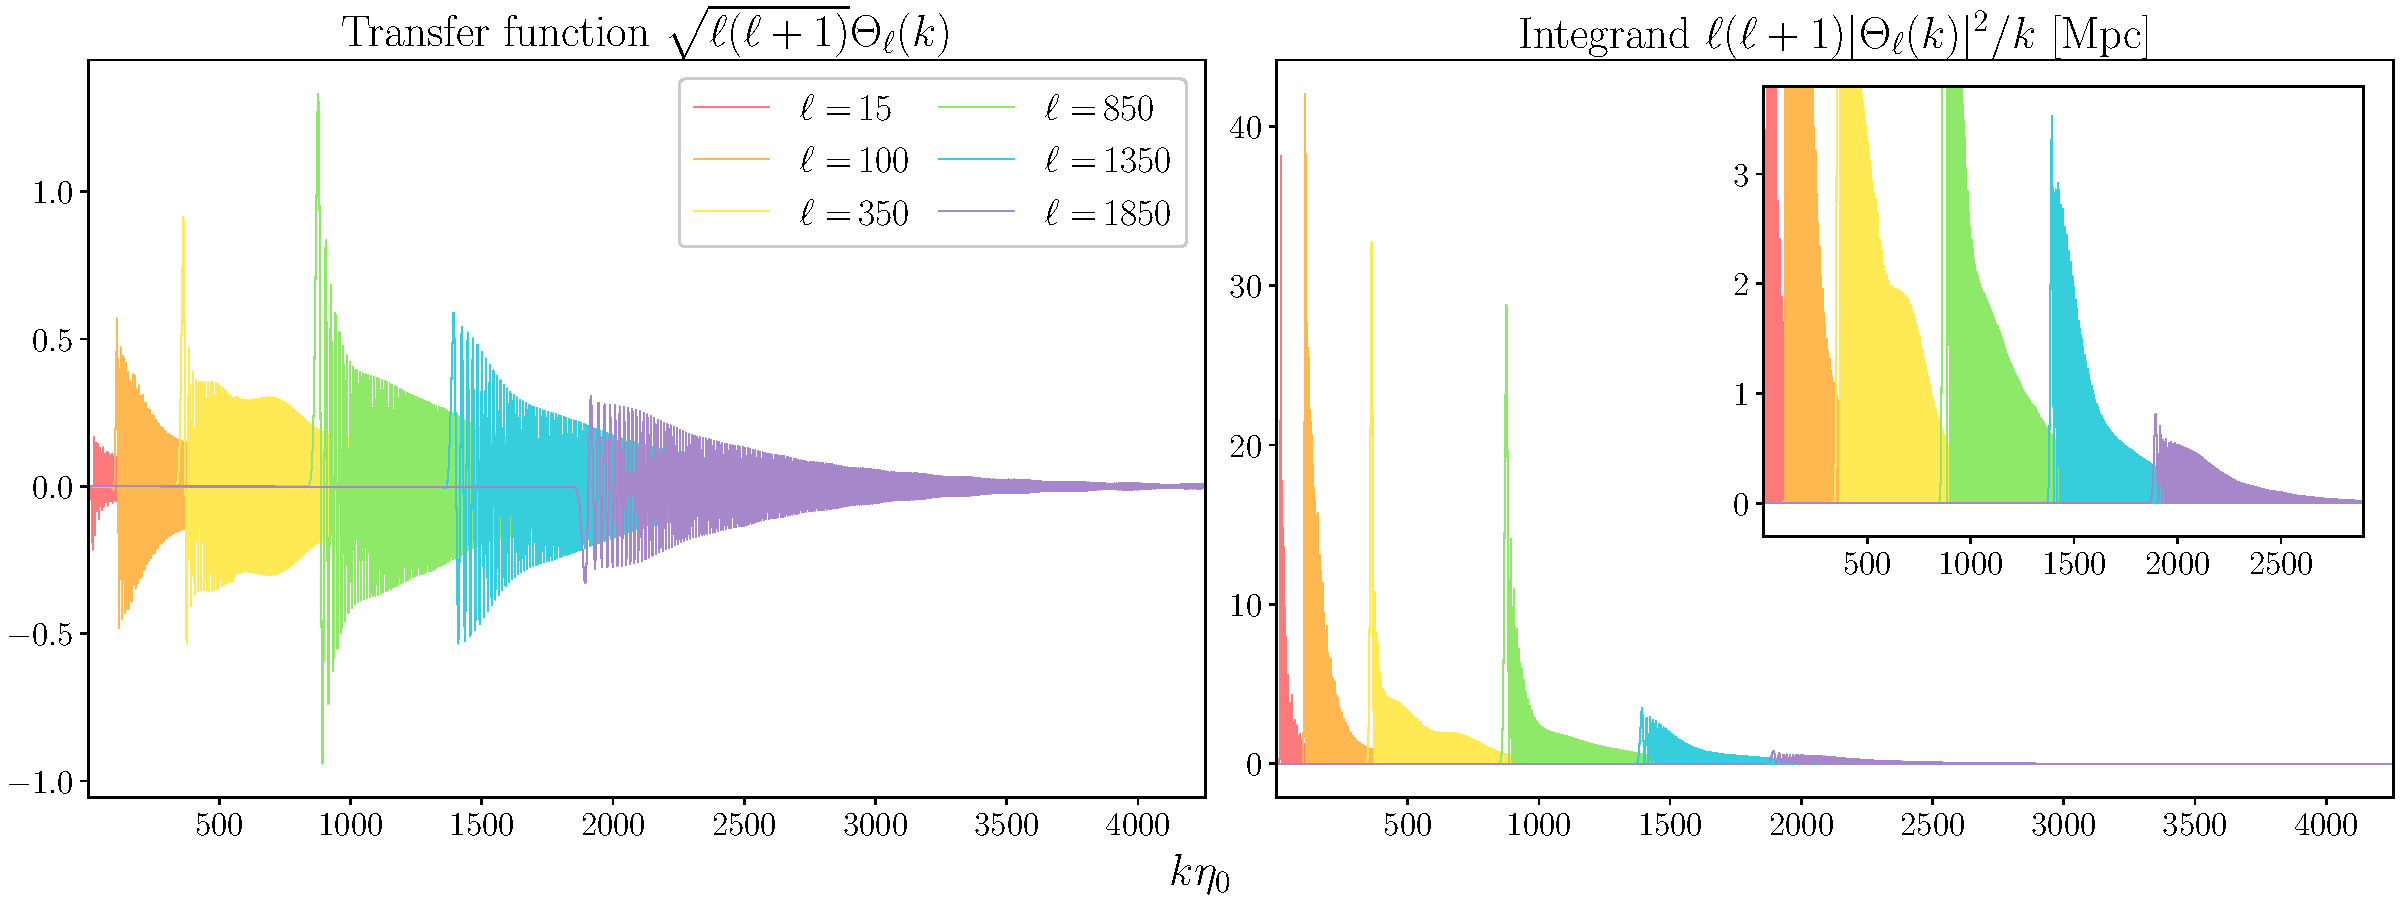
\includegraphics[width=\textwidth]{/Users/paljettrosa/Documents/GitHub/AST5220/figs/transfer_function.pdf}
  \caption{The transfer function $\Theta_\ell(k)$ (left) and the integrand $|\Theta_\ell(k)|^2/k$ (right) for selected multipoles $\ell$. The transfer function describes the projection of primordial perturbations onto angular scales today, while the integrand determines the contribution of each mode $k$ to the angular power spectrum $C_\ell$. \colorbox{Plum}{TODO: maybe change}}\label{fig:transfer function}
\end{figure*}

Figure \ref{fig:transfer function} presents the transfer function $\Theta_\ell(k)$ (left panel) and the integrand of the CMB angular power spectrum integral $|\Theta_\ell(k)|^2 / k$ (right panel), evaluated for a range of multipoles $\ell$. For clarity and better comparison across $\ell$, the left panel is scaled by $\sqrt{\ell(\ell+1)}$ and the right panel by $\ell(\ell+1)$, making the relative contributions more visually apparent.

% The transfer functions $\Theta_\ell(k)$ describe how primordial perturbations at wavenumber $k$ are projected onto angular scale $\ell$. These oscillatory structures reflect acoustic oscillations in the photon-baryon fluid prior to recombination, and their frequency increases with $\ell$, corresponding to finer angular scales. As expected, we see that higher $\ell$-values are sensitive to smaller physical scales (higher $k$) due to their tighter angular resolution on the sky.

% The right panel shows the quantity $\ell(\ell+1)|\Theta_\ell(k)|^2 / k$, which appears in the integral for $C_\ell$. 
In both subplots, the curves reveal where in $k$-space the dominant contributions to the temperature anisotropies arise. We see that as $\ell$ increases, the peak of the integrand shifts to higher $k$, confirming that small-scale modes predominantly source high-$\ell$ power. This is consistent with the approximate projection relation $k \sim \ell/\eta_0$, and illustrates the relationship between spatial and angular scales in cosmological perturbation theory. It also highlights key features that shape the observed spectrum $C_\ell$, such as the oscillatory structure and damping at small scales. \colorbox{Plum}{TODO: maybe change}
% where $\eta_0$ is the comoving distance to the surface of last scattering.


\subsubsection{The CMB temperature power spectrum}

\begin{figure*}
  \centering
  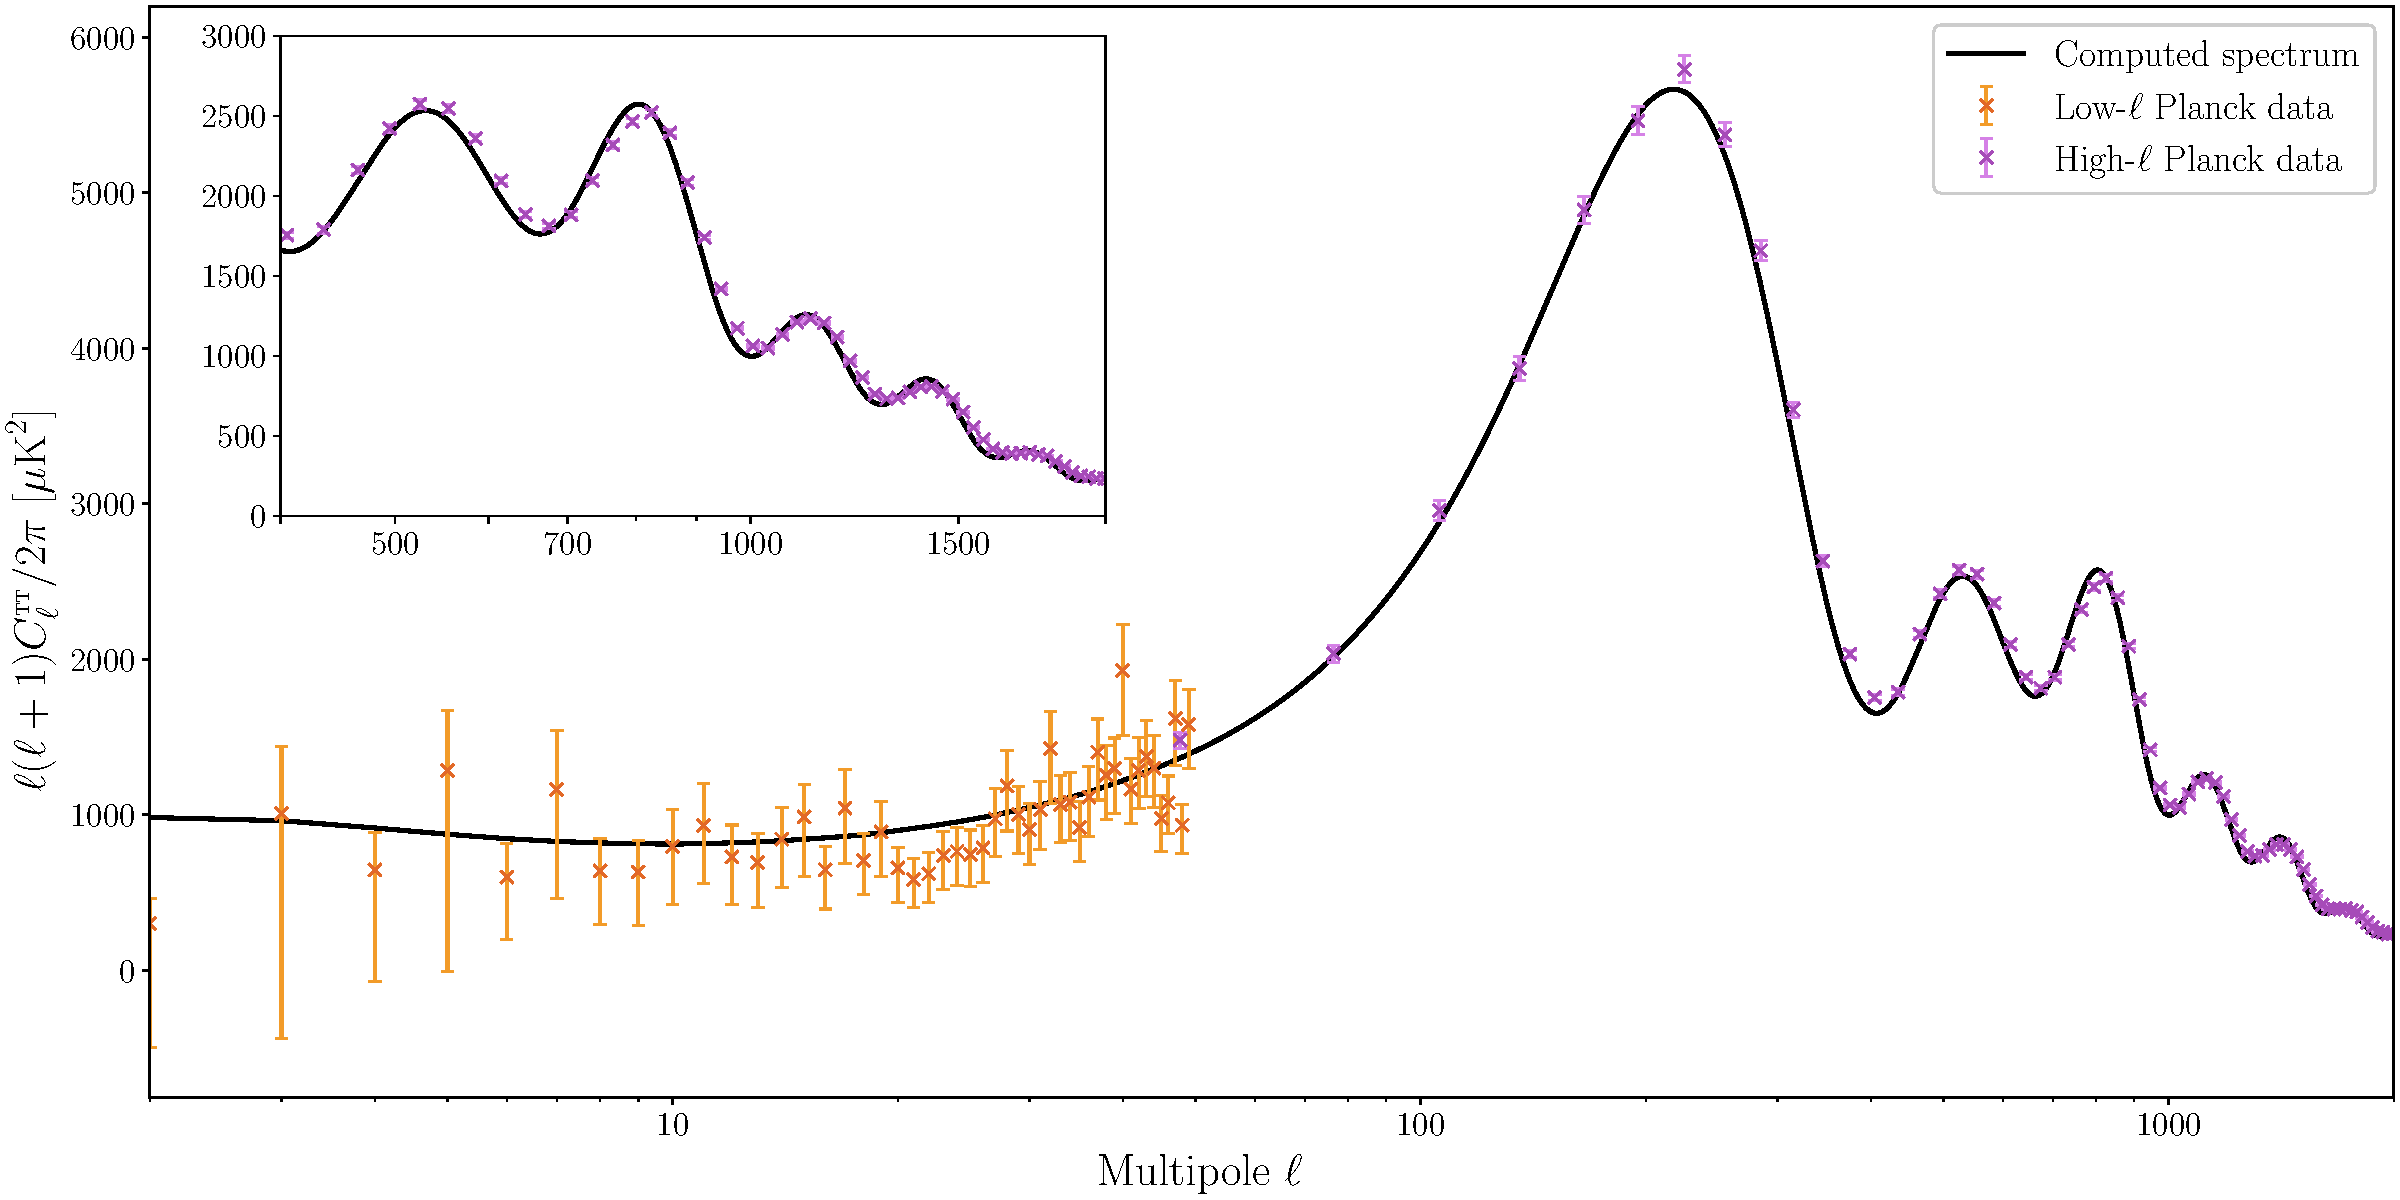
\includegraphics[width=\textwidth]{/Users/paljettrosa/Documents/GitHub/AST5220/figs/CMB.pdf}
  \caption{The CMB temperature power spectrum $C_\ell^\text{TT}$ (black) compared with Planck low-$\ell$ (orange) and high-$\ell$ (purple) data points. The inset highlights a zoom on the high-$\ell$ region. The first three peaks are clearly visible, and the agreement with data is overall good, though the computed peaks are slightly higher, likely due to the absence of gravitational lensing smoothing. \colorbox{Plum}{TODO: maybe change}}\label{fig:CMB}
\end{figure*}

Figure \ref{fig:CMB} presents the final CMB temperature power spectrum $C_\ell^\text{TT}$ computed using the line-of-sight formalism discussed in section \ref{subsubsec: IV theory LOS}, plotted with conventional normalization in units of $\mu\text{K}^2$. Superimposed are the observational data from the Planck satellite, with orange error bars representing low-$\ell$ data and purple bars corresponding to high-$\ell$ measurements. The inset in the top-left corner shows a magnified view of the high-$\ell$ region.

The spectrum exhibits the well-known acoustic peak structure, arising from oscillations in the tightly coupled photon-baryon plasma prior to recombination (see section \ref{subsubsec: IV theory features}). The first peak at $\ell \sim 220$ corresponds to modes that underwent a full compression phase, while subsequent peaks correspond to higher harmonics. As expected, the odd-numbered peaks are amplified due to baryon loading, and the relative suppression of even-numbered peaks encodes the baryon-to-photon ratio. These features are direct consequences of the physics described by the harmonic oscillator formulation of the photon monopole perturbation in the presence of gravity and baryons.

% \color{Plum}
% Additionally, the rising envelope of the acoustic peaks is shaped by radiation driving—an enhancement in oscillation amplitude for modes that enter the horizon during radiation domination, due to the decay of the gravitational potential $\Psi$. This mechanism is detailed in the oscillator analysis in section~5.4 and leads to greater power at higher $\ell$.

% Beyond $\ell \gtrsim 800$, the spectrum exhibits an exponential decline due to diffusion damping (or Silk damping), caused by photon diffusion erasing anisotropies on small angular scales. The suppression is well captured by the damping envelope $D(k) \sim \exp[-(k/k_D)^2]$, where the damping scale $k_D$ depends sensitively on the baryon density and ionization history.

% At large scales ($\ell \lesssim 50$), the spectrum approaches the Sachs-Wolfe plateau, reflecting temperature anisotropies from photons climbing out of static gravitational potential wells on super-horizon scales. The fluctuations here are mostly due to gravitational redshift and are nearly scale-invariant, consistent with a primordial spectrum with $n_s \approx 1$. As noted in section~5.1, this regime suffers from large uncertainties due to cosmic variance, which arises from the limited number of independent modes available on large angular scales. This intrinsic statistical limitation explains the significant spread in the low-$\ell$ Planck data points, despite high instrumental precision.

% The computed spectrum generally agrees well with the Planck data across all scales. However, the zoomed-in subplot reveals that the theoretical peaks are somewhat sharper and taller than observed. This discrepancy is likely due to our neglect of gravitational lensing, which was not included in the current computation. As discussed in section~5.7, lensing deflects CMB photons along their trajectories, smoothing the acoustic peaks by transferring power between neighboring multipoles. Including lensing in the calculation would slightly suppress the peak heights and reduce their sharpness, improving the agreement with observational data.

% Overall, the successful reproduction of the CMB power spectrum—including its peak structure, damping tail, and large-scale behavior—confirms the accuracy of the underlying physical model and numerical implementation. The small discrepancies provide a useful indication of secondary effects, such as lensing, that become important for high-precision cosmology.
% \color{black}

\colorbox{Plum}{TODO: we treat neutrinos as massless?}

\colorbox{Plum}{TODO: truncating the hierarchy too early?}

\begin{figure}
  \centering
  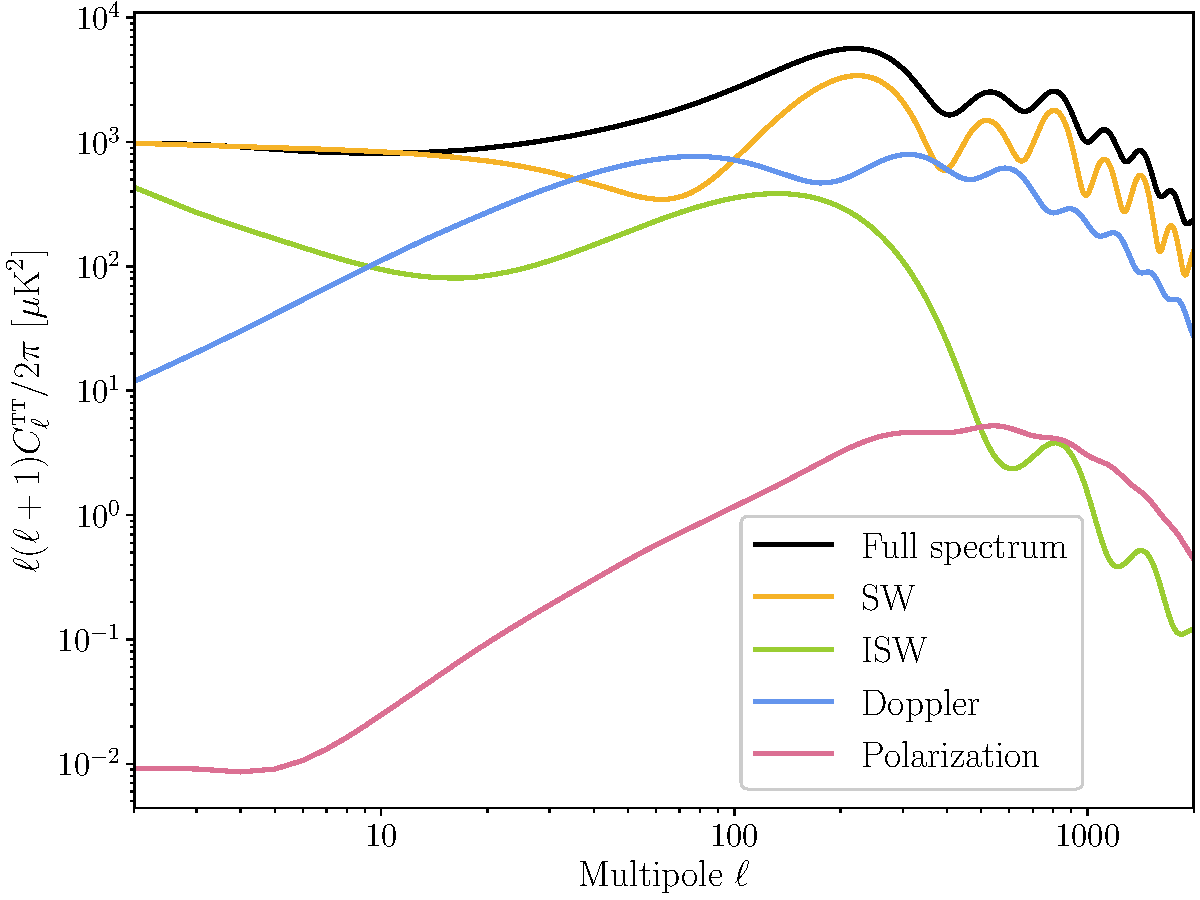
\includegraphics[width=\columnwidth]{/Users/paljettrosa/Documents/GitHub/AST5220/figs/CMB_contributions.pdf}
  \caption{Breakdown of the individual contributions to the CMB temperature power spectrum. The Sachs-Wolfe term (orange) dominates on large scales, the Doppler term (blue) modulates intermediate scales, and the ISW term (green) adds power at low $\ell$. The polarization contribution (red) is subdominant. The full spectrum (black) reflects the coherent sum of all these effects. \colorbox{Plum}{TODO: maybe change}}\label{fig:CMB contributions}
\end{figure}

% \color{Plum}
% Figure \ref{fig:CMB contributions} shows how the total temperature power spectrum is built up from individual physical effects encoded in the source function $\tilde{S}(k,x)$, as defined in section~5.2. Each colored curve corresponds to a spectrum computed using only one component of the source function, allowing us to isolate their impact on the observed CMB anisotropies.

% The Sachs-Wolfe (SW) contribution (orange) dominates the low-$\ell$ (large angular scale) portion of the spectrum, generating the Sachs-Wolfe plateau discussed in section~5.3. This effect arises from the gravitational redshifting of photons climbing out of potential wells at the last scattering surface and is responsible for most of the signal for $\ell \lesssim 30$.

% The integrated Sachs-Wolfe (ISW) term (green) adds to this low-$\ell$ signal and slightly boosts power on the largest angular scales. This term arises due to time variations in the gravitational potentials along the line of sight, particularly relevant during periods of radiation domination and dark energy domination when potential wells evolve. The ISW effect is especially pronounced at very low $\ell$, consistent with the expectations from evolving $\Phi$ and $\Psi$ after matter-radiation and matter-dark energy equality.

% The Doppler contribution (blue), arising from velocity gradients in the photon-baryon fluid at recombination, contributes most strongly at intermediate $\ell$ (around the first few peaks), helping to lift troughs between acoustic peaks. While it does not by itself produce sharp peak structure, it modulates the amplitude of oscillations and adds to the overall spectrum in a scale-dependent way.

% The polarization contribution (red) is generally small, but becomes more important at higher multipoles. It originates from anisotropic Thomson scattering during recombination and reionization, affecting the quadrupole of the photon distribution and hence contributes to both temperature and polarization anisotropies.

% Finally, the full spectrum (black) is obtained by summing over all terms in the source function. It exhibits the complete series of acoustic peaks, with precise structure arising from the interplay of all contributing effects. The difference in magnitude between the full spectrum and any single component underscores the necessity of including all physical contributions to accurately model the CMB anisotropies.

% This decomposition clearly shows how different physical mechanisms contribute across scales: gravitational effects dominate large scales, velocity effects modulate the intermediate range, and polarization and damping features become more relevant at small angular scales. It also highlights the importance of each term in shaping the structure of $C_\ell^\text{TT}$, as explored throughout milestone IV.
% \color{black}


\subsubsection{TE and EE polarization power spectra}

\begin{figure*}
  \centering
  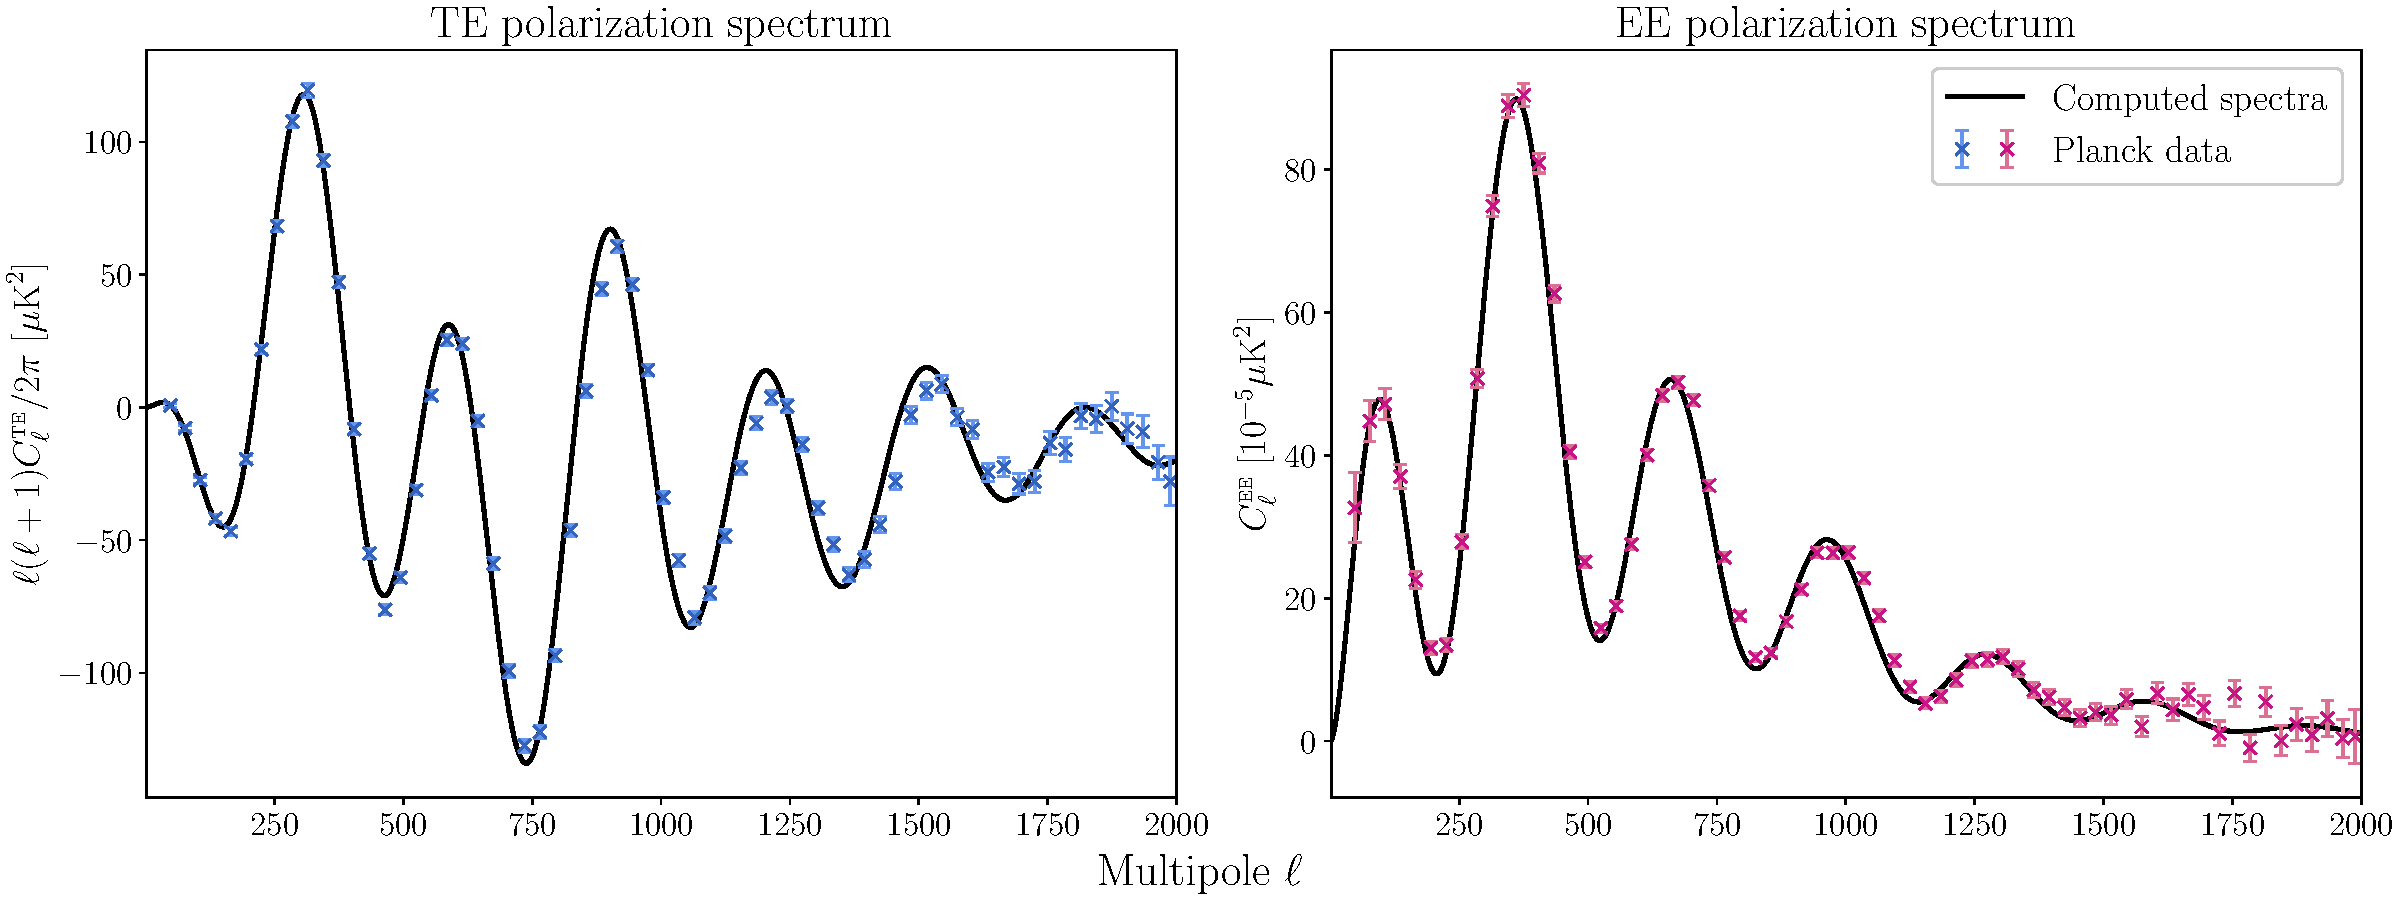
\includegraphics[width=\textwidth]{/Users/paljettrosa/Documents/GitHub/AST5220/figs/polarization_spectra.pdf}
  \caption{The CMB TE (left) and EE (right) polarization spectra compared with high-$\ell$ data. The computed spectra reproduce the oscillatory features seen in the data, though the amplitude is somewhat larger and the TE peaks slightly shifted in $\ell$, likely due to the neglect of gravitational lensing. \colorbox{Plum}{TODO: maybe change}}\label{fig:polarization spectra}
\end{figure*}

% \color{Plum}
% In figure \ref{fig:polarization spectra}, I present the CMB temperature-polarization cross-power spectrum ($C_\ell^\text{TE}$, left) and the E-mode polarization auto-power spectrum ($C_\ell^\text{EE}$, right). Both spectra are shown with high-$\ell$ Planck data points overlaid with error bars. These polarization spectra complement the temperature (TT) spectrum by providing additional constraints on the early Universe physics and breaking degeneracies between cosmological parameters.

% As discussed in section \colorbox{Plum}{TODO: theory ref}, the E-mode polarization arises primarily from the quadrupole anisotropy in the photon distribution at the time of recombination, induced by velocity gradients in the photon-baryon fluid. The TE spectrum measures the correlation between these polarization patterns and temperature fluctuations, while the EE spectrum quantifies the variance of the polarization signal itself.

% The TE spectrum exhibits a characteristic oscillatory pattern that is out of phase with the TT spectrum due to the different sources of temperature and polarization fluctuations. In the left panel, the computed $C_\ell^\text{TE}$ spectrum agrees qualitatively with the Planck data across the full multipole range, showing alternating peaks and troughs consistent with acoustic oscillations. However, the theoretical prediction appears to be slightly shifted toward lower $\ell$ compared to the data, especially around the peak regions. This shift may suggest a minor mismatch in the acoustic scale, possibly due to simplified assumptions in the background evolution or missing physical effects such as gravitational lensing.

% In the EE spectrum (right panel), the predicted peak structure again aligns well with the general trend in the data. Nevertheless, as with the TT and TE spectra, the computed EE spectrum exhibits slightly higher peak amplitudes compared to observations. One plausible explanation, as discussed in the previous section, is the omission of gravitational lensing effects. Lensing redistributes power by smoothing out the acoustic peaks in all CMB spectra, including TT, TE, and EE. This effect leads to slightly lower and broader peaks in the observed spectra, an effect clearly seen in the high-$\ell$ Planck data and absent in our unlensed predictions.

% Other possible contributors to these discrepancies include inaccuracies in the ionization history (e.g., assumptions in the reionization model), numerical inaccuracies in the Boltzmann hierarchy integration, or simplifications in the polarization source function. Overall, however, the spectra reproduce the expected physical features with good qualitative agreement and capture the core signatures of the polarization anisotropies.
% \color{black}


\subsubsection{The neutrino power spectrum}

\begin{figure}
  \centering
  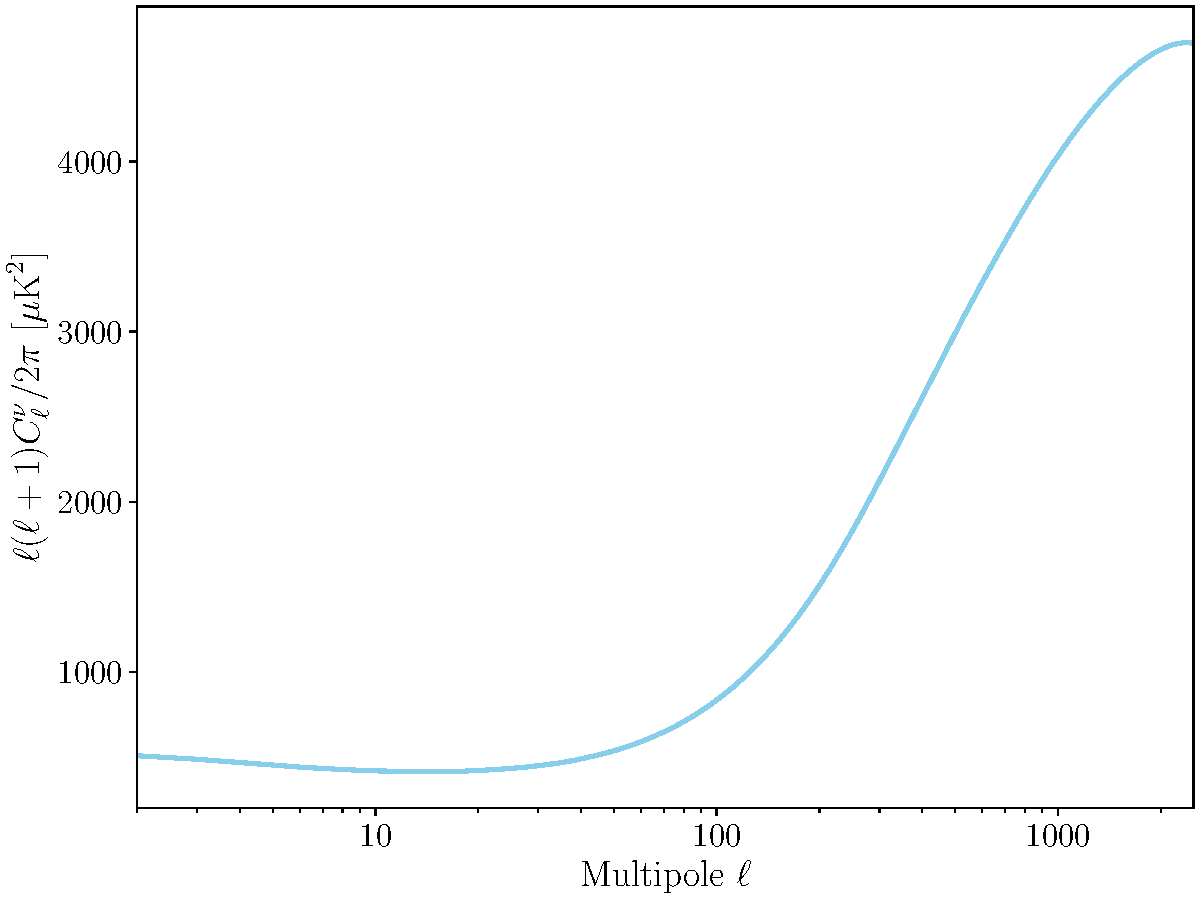
\includegraphics[width=\columnwidth]{/Users/paljettrosa/Documents/GitHub/AST5220/figs/neutrino_spectrum.pdf}
  \caption{The neutrino angular power spectrum $C_\ell^\nu$, computed using the same conventions as the CMB temperature spectrum. Although unobservable, the spectrum illustrates the effects of free-streaming relativistic particles and includes only Sachs-Wolfe and ISW contributions. \colorbox{Plum}{TODO: spectrum looks wrong}}\label{fig:neutrino spectrum}
\end{figure}

% \color{Plum}
% Figure \ref{fig:neutrino spectrum} shows the angular power spectrum of the cosmic neutrino background (CNB) temperature anisotropies, $C_\ell^\nu$, calculated using the same normalization as for the CMB spectrum—except using the neutrino temperature instead of the photon temperature. Although this spectrum is not observable in practice due to the extremely weak interactions of neutrinos, it still provides valuable theoretical insights.

% As discussed in section \colorbox{Plum}{TODO: theory ref}, the evolution of neutrino perturbations is simpler than that of photons, owing to their decoupling in the very early Universe. The neutrino source function includes only two terms: a Sachs-Wolfe term, $\Theta_0^\nu + \Psi$, and an integrated Sachs-Wolfe term, $\Psi' - \Phi'$. This simplicity leads to a much smoother and featureless spectrum compared to the CMB temperature spectrum, which exhibits pronounced acoustic peaks due to the photon-baryon interactions prior to recombination.

% The overall shape of $C_\ell^\nu$ is determined primarily by free-streaming behavior. Since neutrinos decouple while still relativistic, they stream out of overdense regions, suppressing power on small scales (high $\ell$) and leading to the smooth decay seen in the spectrum. The lack of oscillatory features reflects the absence of acoustic oscillations in the neutrino perturbations.

% Furthermore, the relative amplitude of the spectrum is lower than that of the CMB, consistent with the fact that gravitational potentials decay less effectively in a radiation-dominated Universe, and neutrinos contribute only passively to the potential evolution. Unlike the CMB, there is no Doppler or polarization term to modulate the angular structure of $C_\ell^\nu$, and thus its contributions are limited to broader features.
% \color{black}


\subsubsection{The matter power spectrum}

\begin{figure}
  \centering
  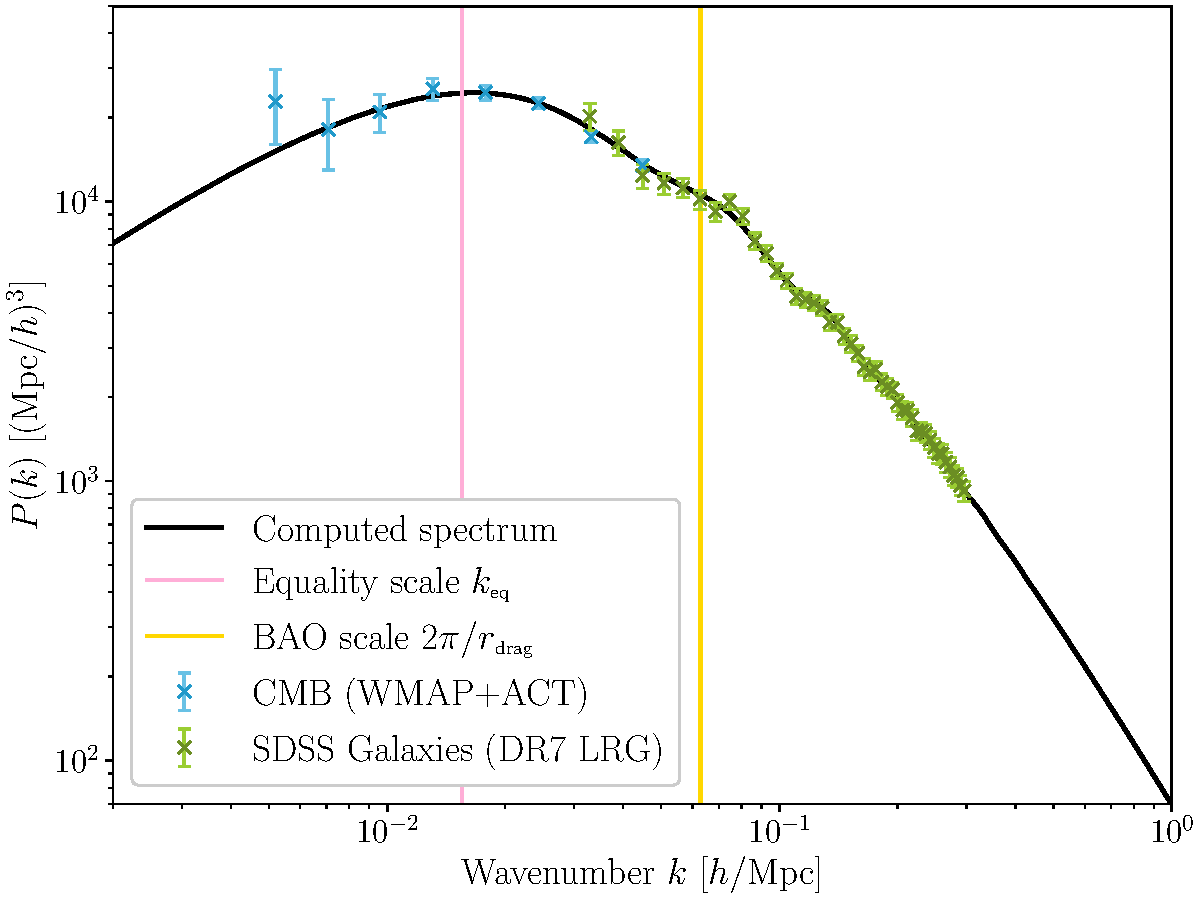
\includegraphics[width=\columnwidth]{/Users/paljettrosa/Documents/GitHub/AST5220/figs/P_k.pdf}
  \caption{Matter power spectrum $P(k)$ in units of (Mpc/$h$)$^3$. Theoretical prediction is compared to WMAP+ACT (blue) and SDSS DR7 LRG (green) data. The model reproduces the overall shape and amplitude well, especially around the BAO feature at $k \sim 0.1\,h$/Mpc. \colorbox{Plum}{TODO: maybe change}}\label{fig:P_k}
\end{figure}

Figure \ref{fig:P_k} shows the matter power spectrum $P(k)$ today, plotted in units of $(\text{Mpc}/h)^3$ as a function of the wavenumber $k$ in $h/\text{Mpc}$. The black curve represents the theoretically computed spectrum, while blue and green error bars show observational data from CMB measurements by the Wilkinson Microwave Anisotropy Probe (WMAP) and the Acatama Cosmology Telescope (ACT), and the Sloan Digital Sky Survey (SDSS) DR7 Luminous Red Galaxies (LRGs), respectively. \colorbox{Plum}{TODO: rephrase}

As detailed in section \ref{subsubsec: IV theory matter}, the shape of the matter power spectrum reflects both the primordial spectrum seeded during inflation and the subsequent growth of perturbations across spatial scales. In particular, the turnover near the scale $k_\text{eq}$ (marked on the plot) corresponds to the mode that entered the horizon at matter-radiation equality. Modes with $k \ll k_\text{eq}$ entered the horizon during matter domination and grew efficiently due to gravitational instability. Conversely, modes with $k \gg k_\text{eq}$ entered during radiation domination, when the rapid expansion and pressure support from relativistic species suppressed growth, resulting in the $\propto k^{-3}$ decline of $P(k)$ at large $k$. 

\colorbox{Plum}{TODO: discuss how the primordial spectrum is visible}

The plot also marks the baryon acoustic oscillation (BAO) scale $2\pi/r_\text{drag}$, which arises from sound waves in the early Universe's photon-baryon fluid and appears as a characteristic scale in both the matter and CMB power spectra. Although the BAO wiggles are less pronounced in the matter power spectrum due to the smoothing effect of nonlinear evolution, they are still visible. \colorbox{Plum}{TODO: change/remove this}

The agreement between the computed spectrum and observational data is generally good across a wide range of scales. On large scales ($k \lesssim 0.1\,h/\text{Mpc}$), the model accurately matches both the CMB and galaxy data, confirming the consistency of the perturbation evolutions with initial inflationary conditions. \colorbox{Plum}{TODO: word different} On smaller scales ($k \gtrsim 0.1\,h/\text{Mpc}$), the slight deviations likely stem from nonlinear clustering effects not captured in our linear treatment. Additionally, galaxy bias and redshift-space distortions introduce observational systematics in the SDSS measurements, which may also contribute to discrepancies. \colorbox{Plum}{TODO: add source}




\section{Conclusions}\label{sec: conclusions}

\bibliographystyle{aa} % style aa.bst
\bibliography{references} % your references Yourfile.bib

\appendix

\onecolumn

\section{Toy cosmology figures}\label{appsec: figures}
% \subsection{Milestone I}\label{appsubsec: fig I}
\begin{figure}[h!]
  \centering
  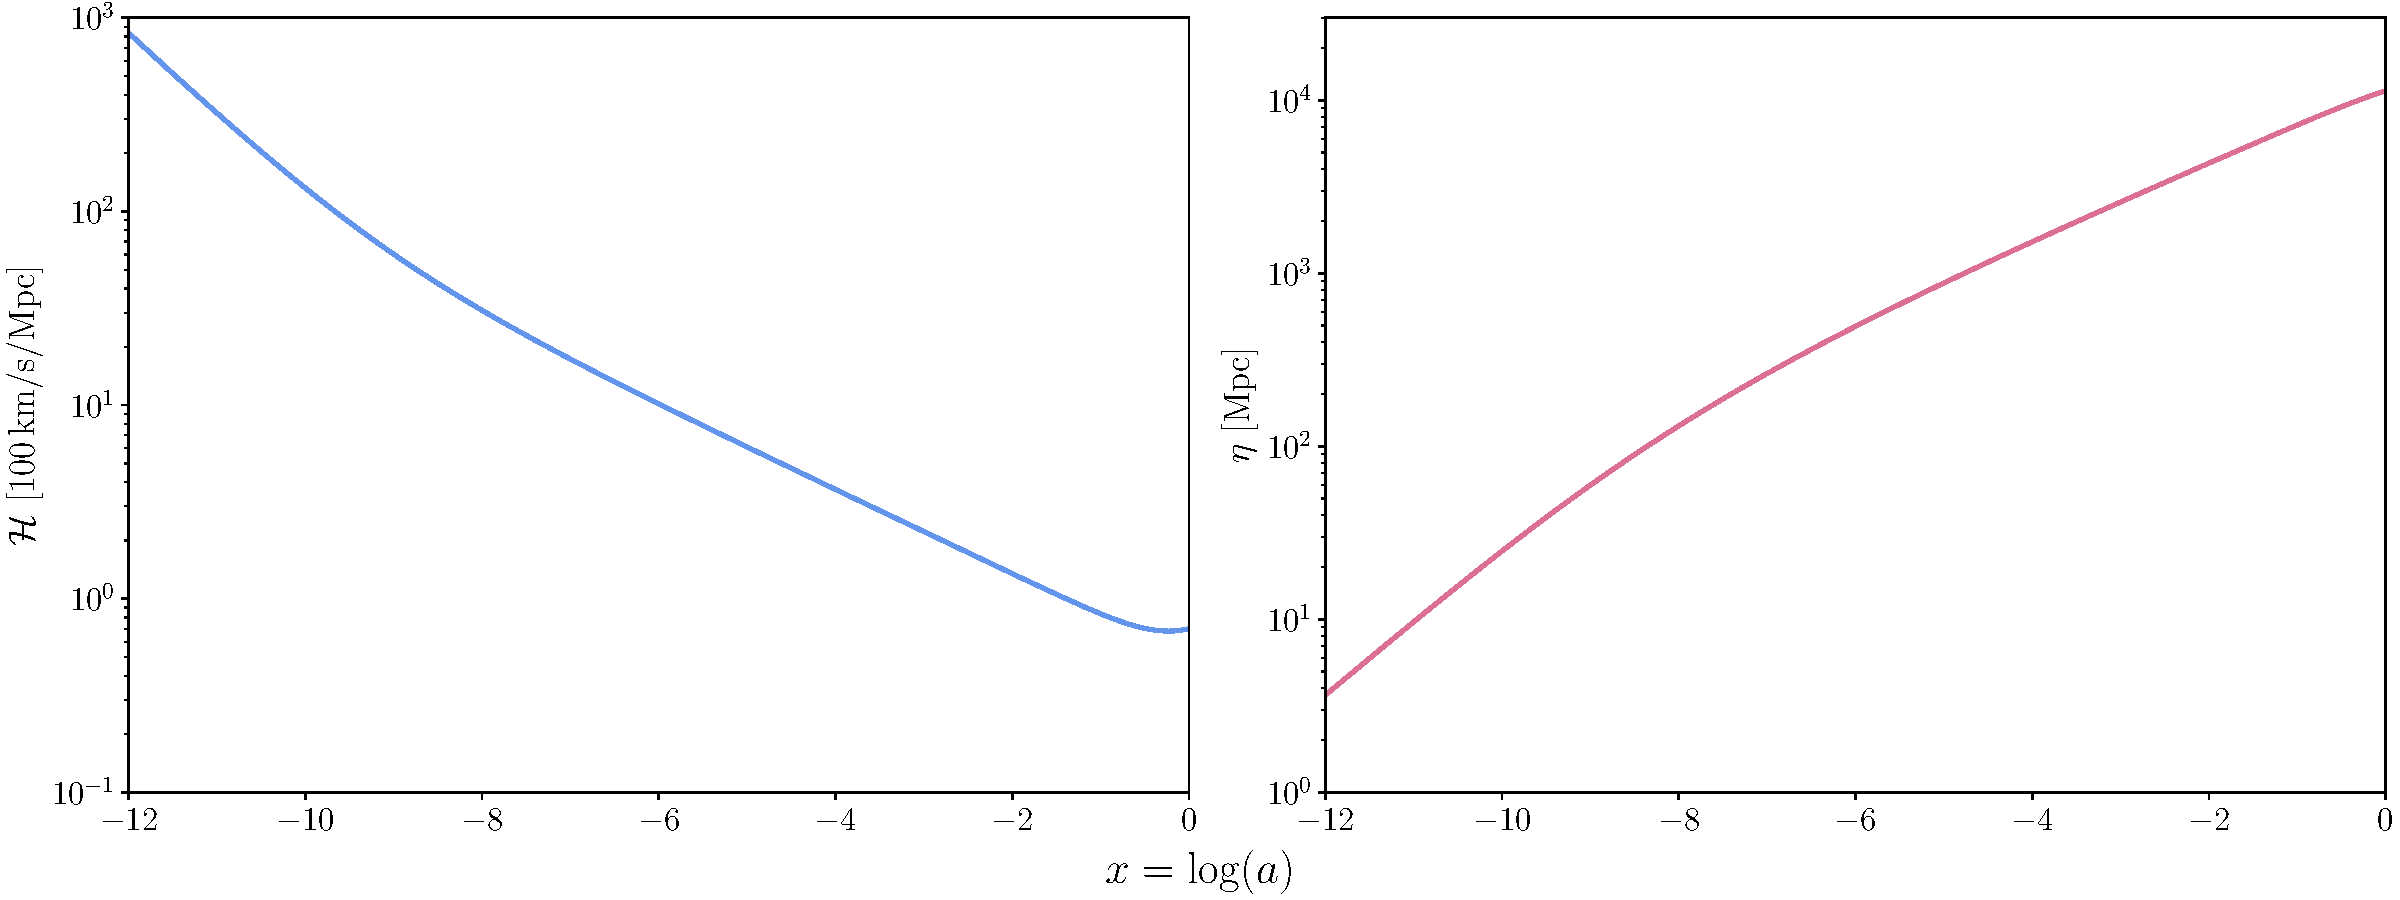
\includegraphics[width=0.95\textwidth]{/Users/paljettrosa/Documents/GitHub/AST5220/figs/toy/Hp_and_eta.pdf}
  \caption{Evolution of the conformal Hubble parameter $\mathcal{H}$ (left) and the conformal time $\eta$ (right) in Winther's toy cosmological model. The parameters used are $h=0.7$, $\Omega_{\text{CDM}0}=0.45$, $\Omega_{b0}=0.05$ and $N_\text{eff}=0$. $\Omega_{k0}$ and $T_\text{CMB0}$ are the same as for the fiducial cosmology.}\label{appfig: Hp_and_eta}
  \vspace{-15pt}
\end{figure}

\begin{figure}[h!]
  \begin{minipage}{0.5\textwidth}
  % \begin{figure}[h!]
    % \vspace{-11pt}
    \centering
    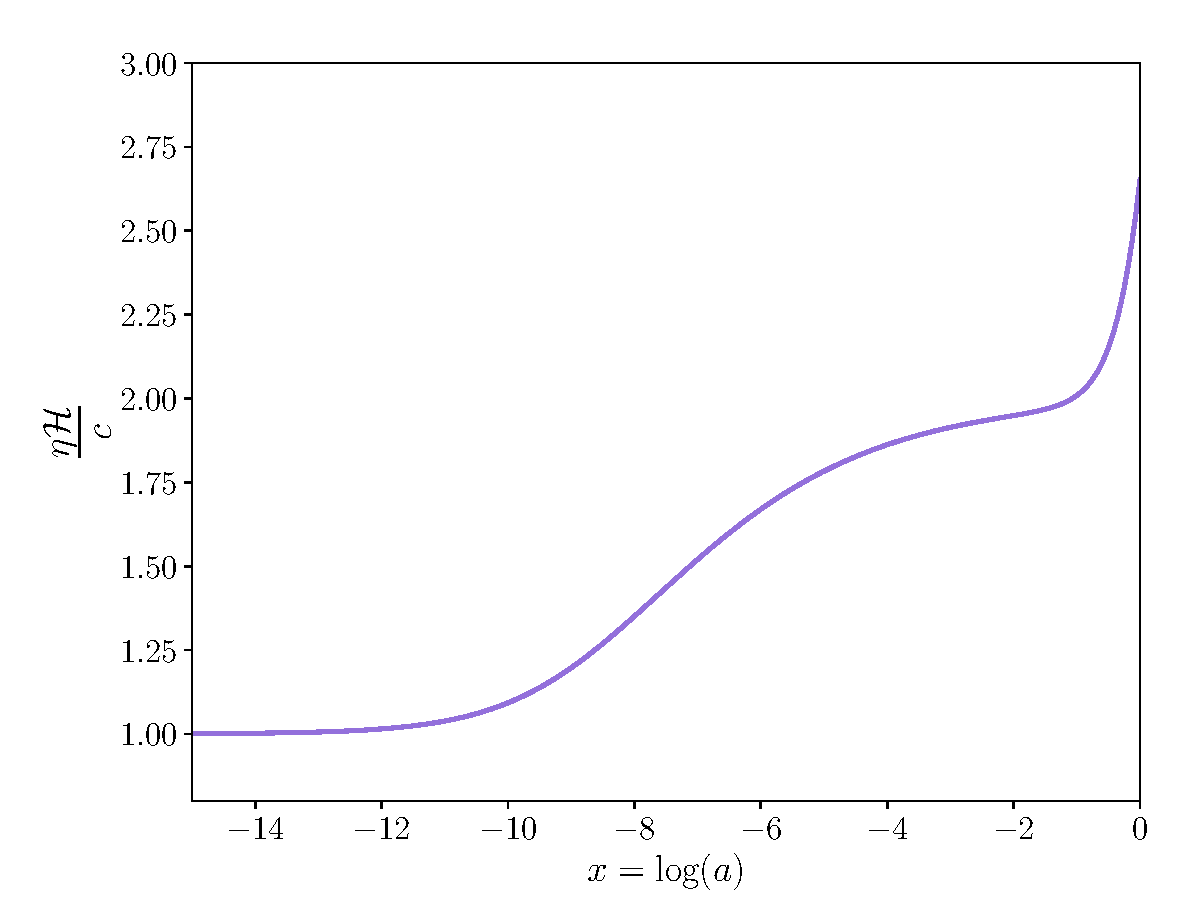
\includegraphics[width=0.95\linewidth]{/Users/paljettrosa/Documents/GitHub/AST5220/figs/toy/eta_Hp_over_c.pdf}
    \caption{Evolution of the ratio $\eta\mathcal{H}/c$ in Winther's toy cosmological\\ model ($h=0.7$, $\Omega_{\text{CDM}0}=0.45$, $\Omega_{b0}=0.05$ and $N_\text{eff}=0$).}\label{appfig: eta_Hp_over_c}
  % \end{figure}
  \end{minipage}
  \begin{minipage}{0.5\textwidth}
  % \begin{figure}[h!]
    % \centering
    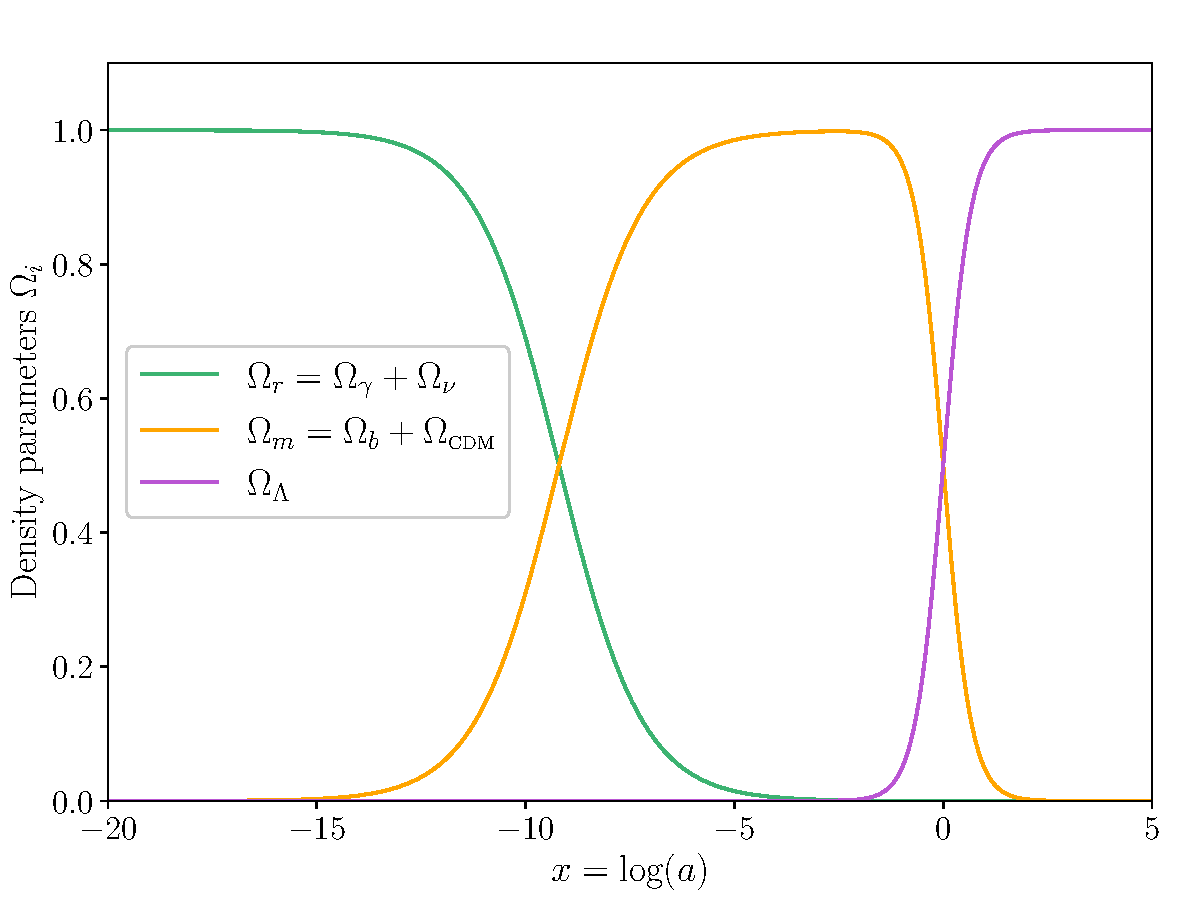
\includegraphics[width=0.95\linewidth]{/Users/paljettrosa/Documents/GitHub/AST5220/figs/toy/Omega_i.pdf}
    % \vspace{-11pt}
    \caption{Evolution of the density parameters $\Omega_r$ (green), $\Omega_m$ (orange) and $\Omega_\Lambda$ (purple) in Winther's toy cosmological model ($h=0.7$, $\Omega_{\text{CDM}0}=0.45$, $\Omega_{b0}=0.05$ and $N_\text{eff}=0$).}\label{appfig: Omega_i}
  % \end{figure}
  \end{minipage}
\vspace{-5pt}
\end{figure}


\begin{figure}[h!]
  % \subsection{Milestone II}\label{appsubsec: fig II}
  \centering
  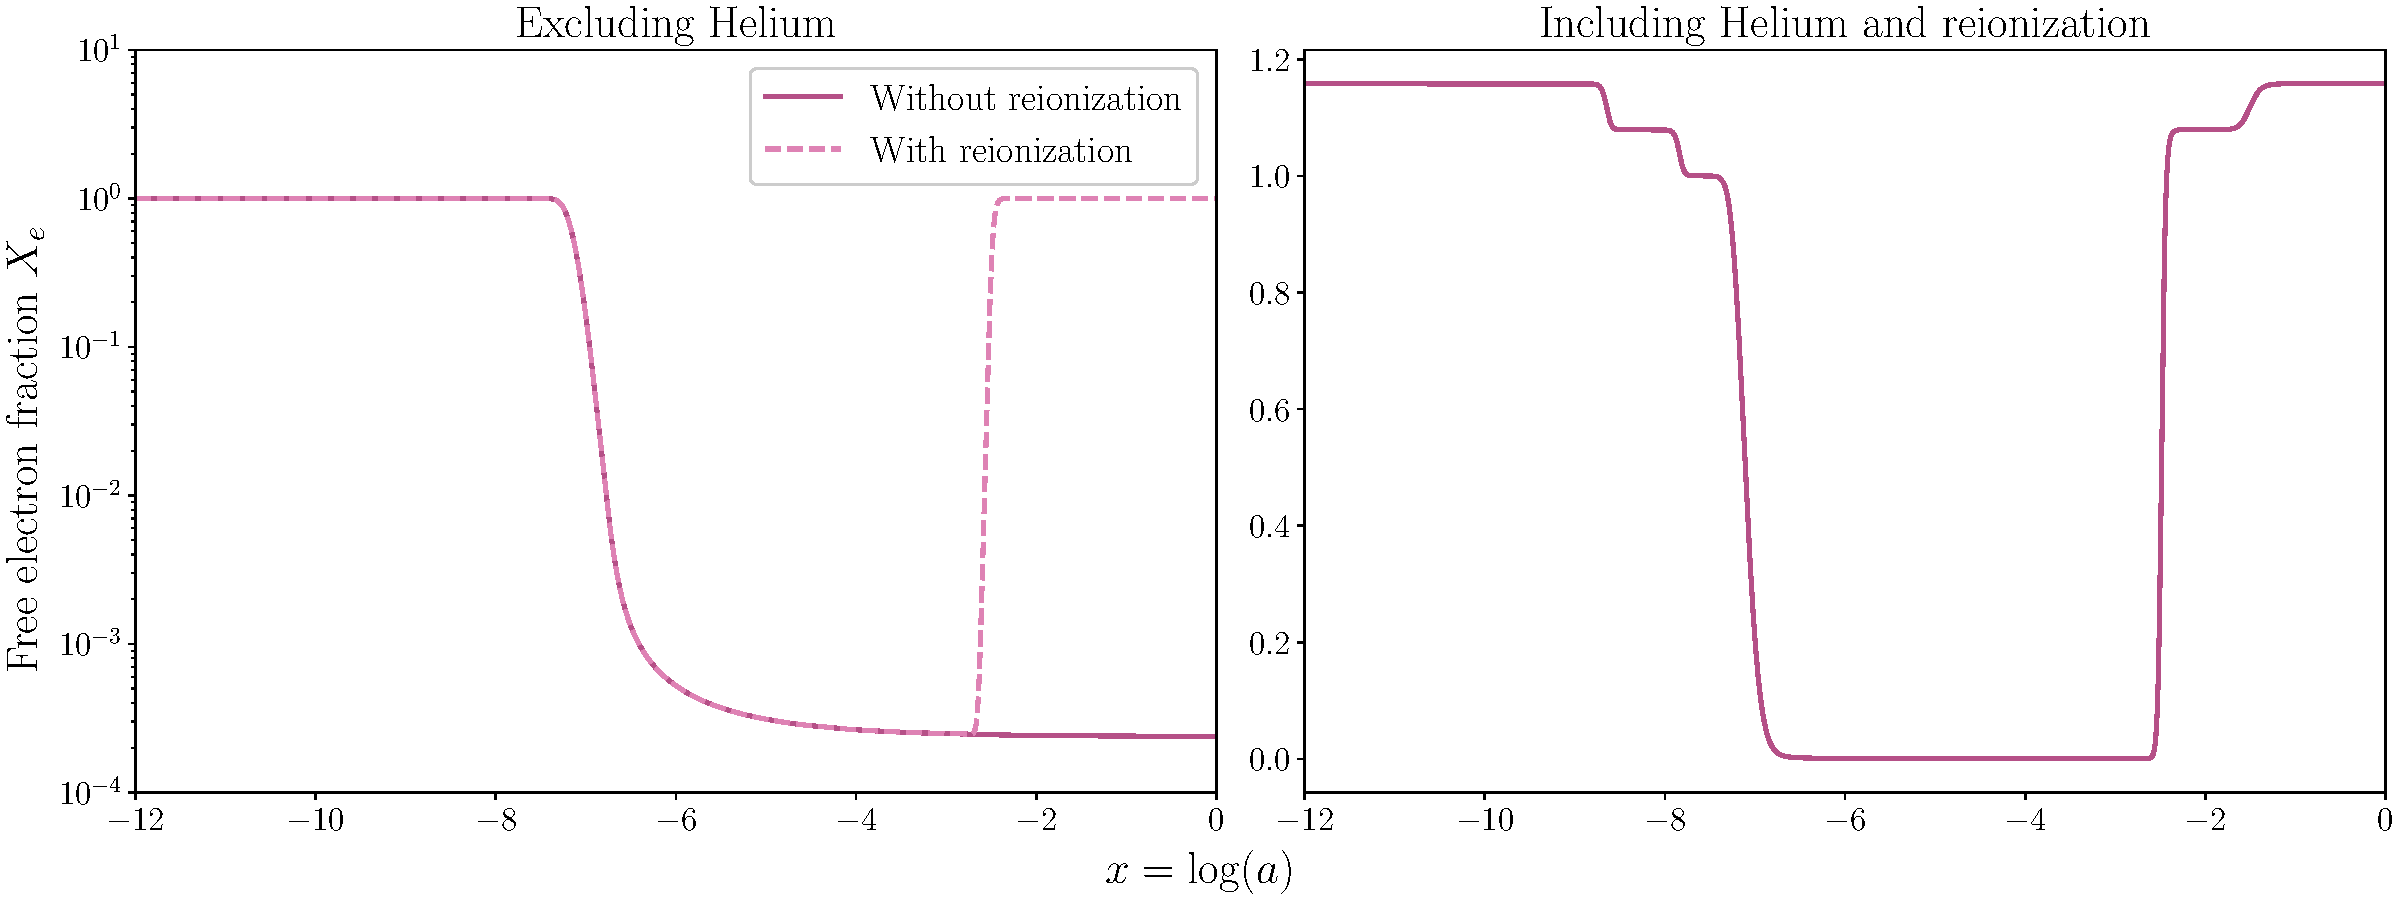
\includegraphics[width=0.95\textwidth]{/Users/paljettrosa/Documents/GitHub/AST5220/figs/toy/Xe.pdf}
  \caption{Evolution of the free electron fraction with (right) and without (left) Helium in Winther's toy cosmological model. The Hydrogen reionization parameters used are $z_\text{reion}=11.0$ and $\Delta z_\text{reion}=0.5$. When including Helium, $Y_p=0.24$ is used as the primordial abundance, and $z_\text{He,reion}=3.5$ and $\Delta z_\text{He,reion}=0.5$ as Helium reionization parameters.}\label{appfig: Xe}
  \vspace{-20pt}
\end{figure}

\newpage

\begin{figure}[h!]
  \centering
  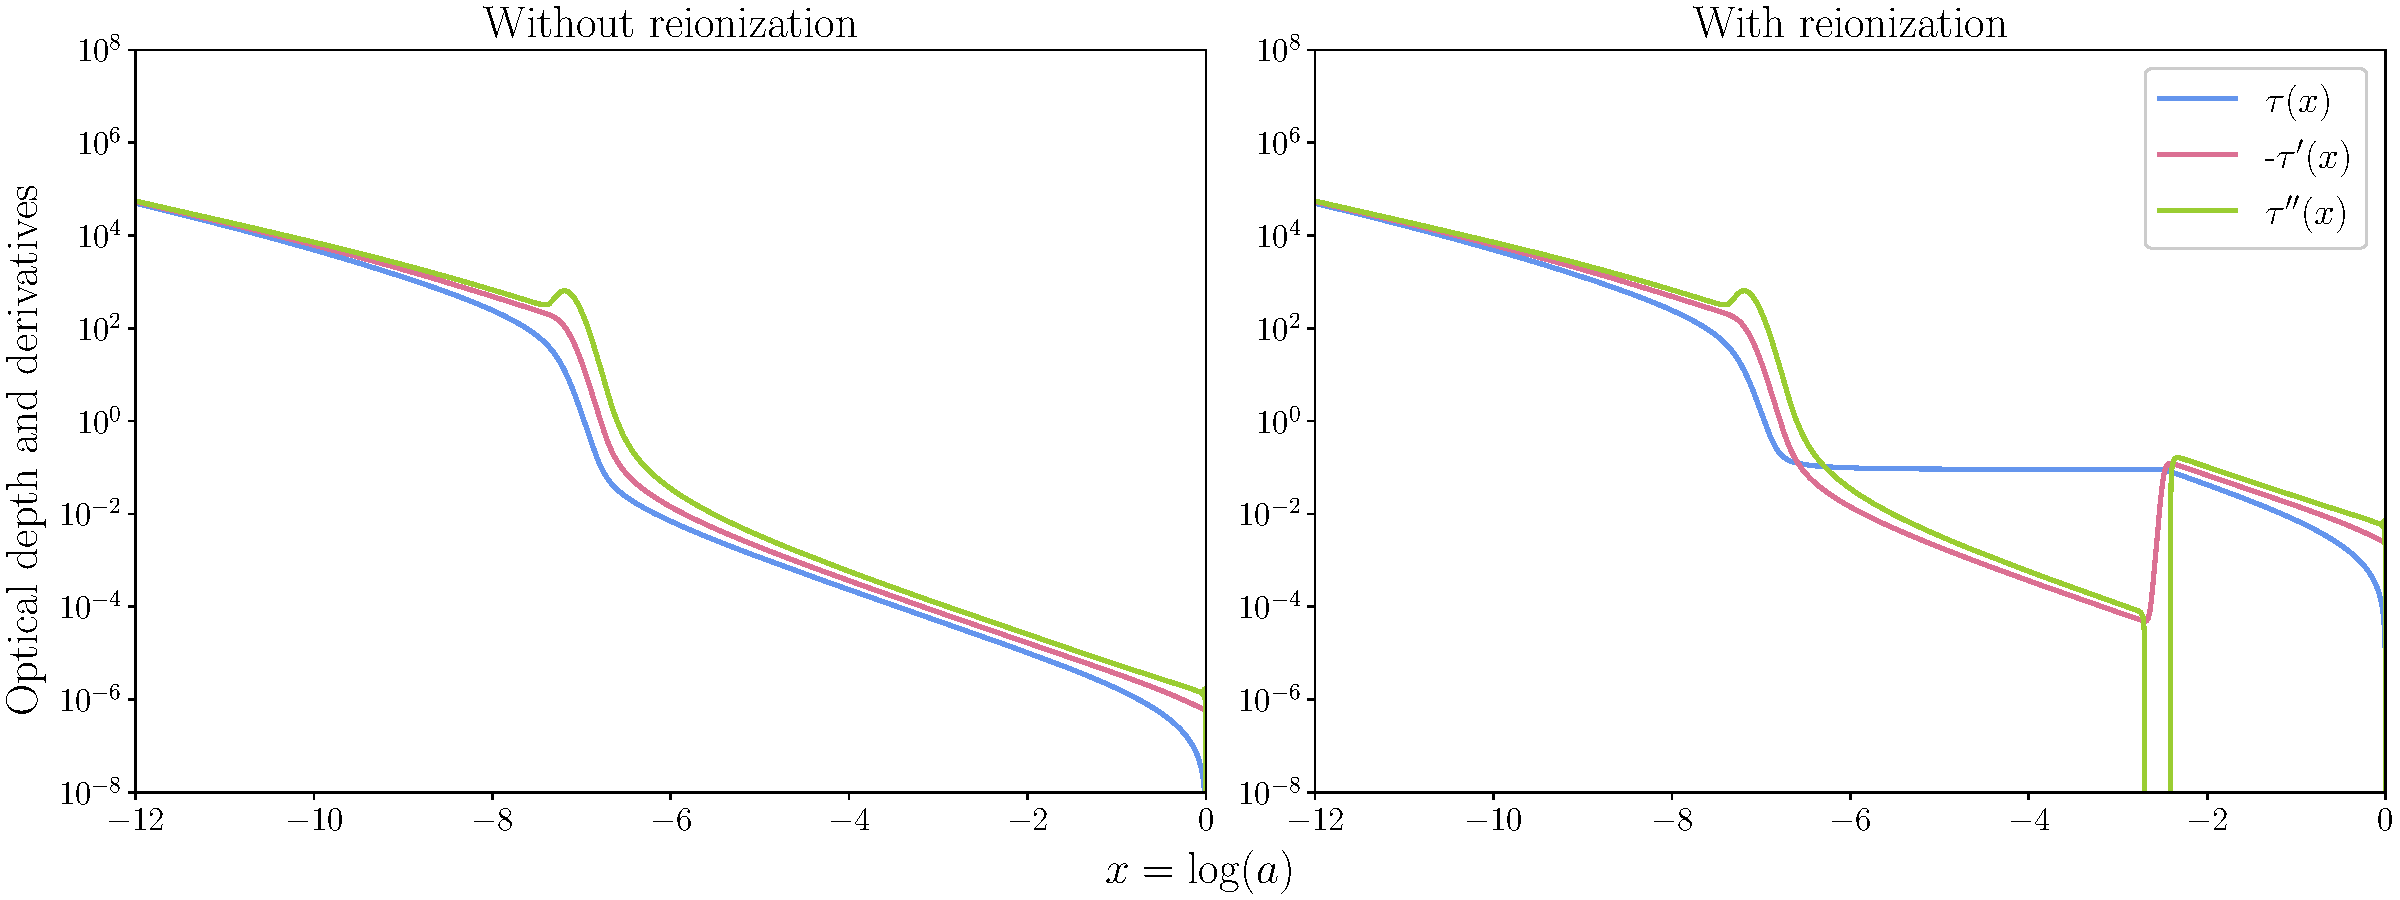
\includegraphics[width=0.95\textwidth]{/Users/paljettrosa/Documents/GitHub/AST5220/figs/toy/tau.pdf}
  \caption{Evolution of the optical depth $\tau$ and derivatives $-\tau'$ and $\tau''$ with (right) and without (left) reionization included in Winther's toy cosmological model. Helium is not included, and the reionization parameters used are $z_\text{reion}=11.0$ and $\Delta z_\text{reion}=0.5$.}\label{appfig: tau}
  \vspace{-10pt}
\end{figure}

\begin{figure}[h!]
  % \vspace{-10pt}
  \begin{minipage}{0.5\textwidth}
    \centering
    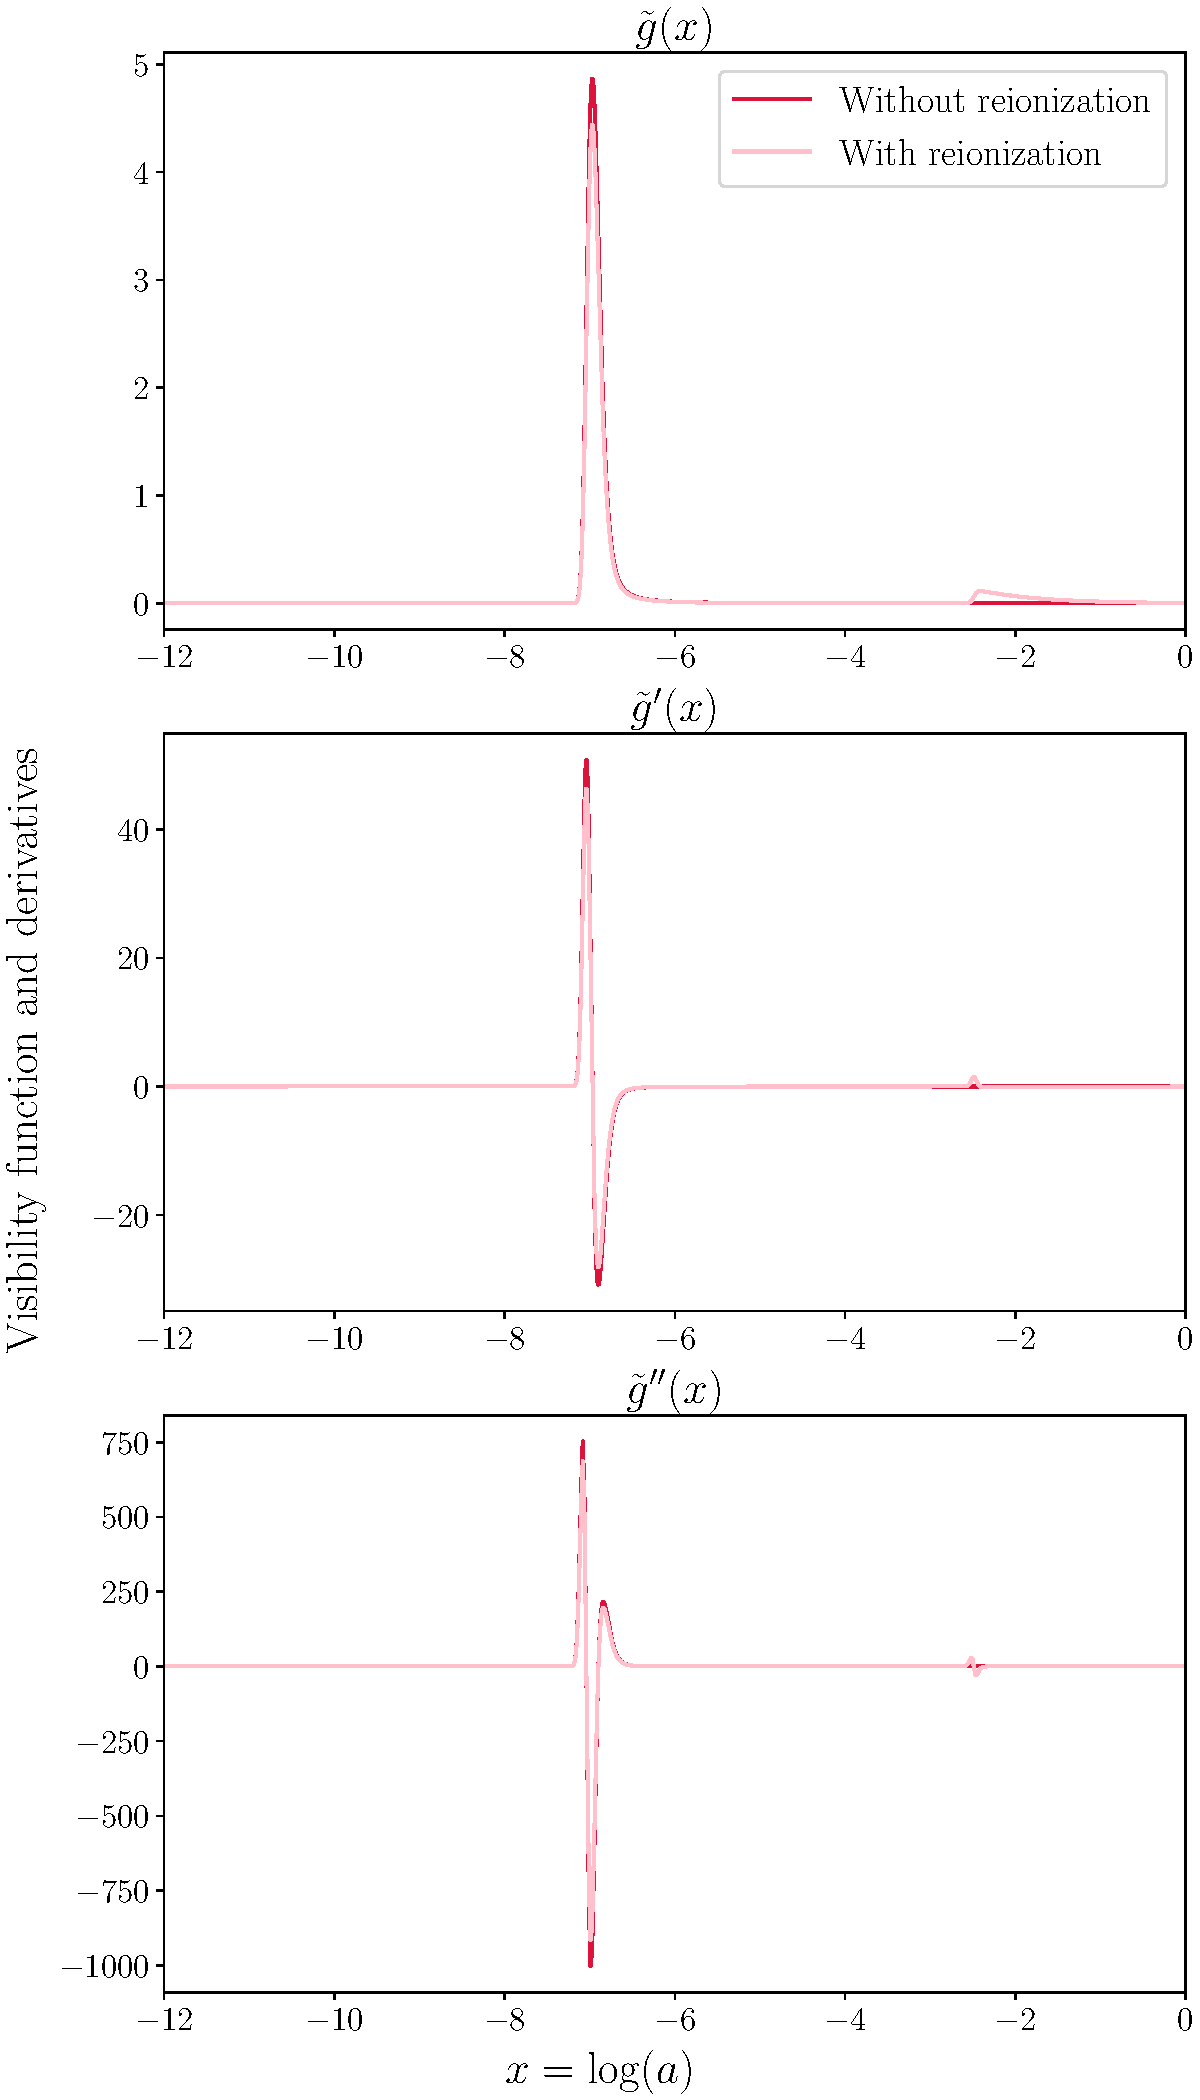
\includegraphics[width=0.95\linewidth]{/Users/paljettrosa/Documents/GitHub/AST5220/figs/toy/g_tilde.pdf}
    \caption{The visibility function $\tilde{g}$ (top) and its first (middle) and second (bottom) derivatives $\tilde{g}'$ and $\tilde{g}''$ in Winther's toy cosmological model, plotted with (pink) and without (red) reionization. Helium is not included, and the reionization parameters are $z_\text{reion}=11.0$ and $\Delta z_\text{reion}=0.5$.}\label{appfig: g_tilde}
  \end{minipage}
  \begin{minipage}{0.5\textwidth}
    % \subsection{Milestone III}\label{appsubsec: fig III}
    \centering
    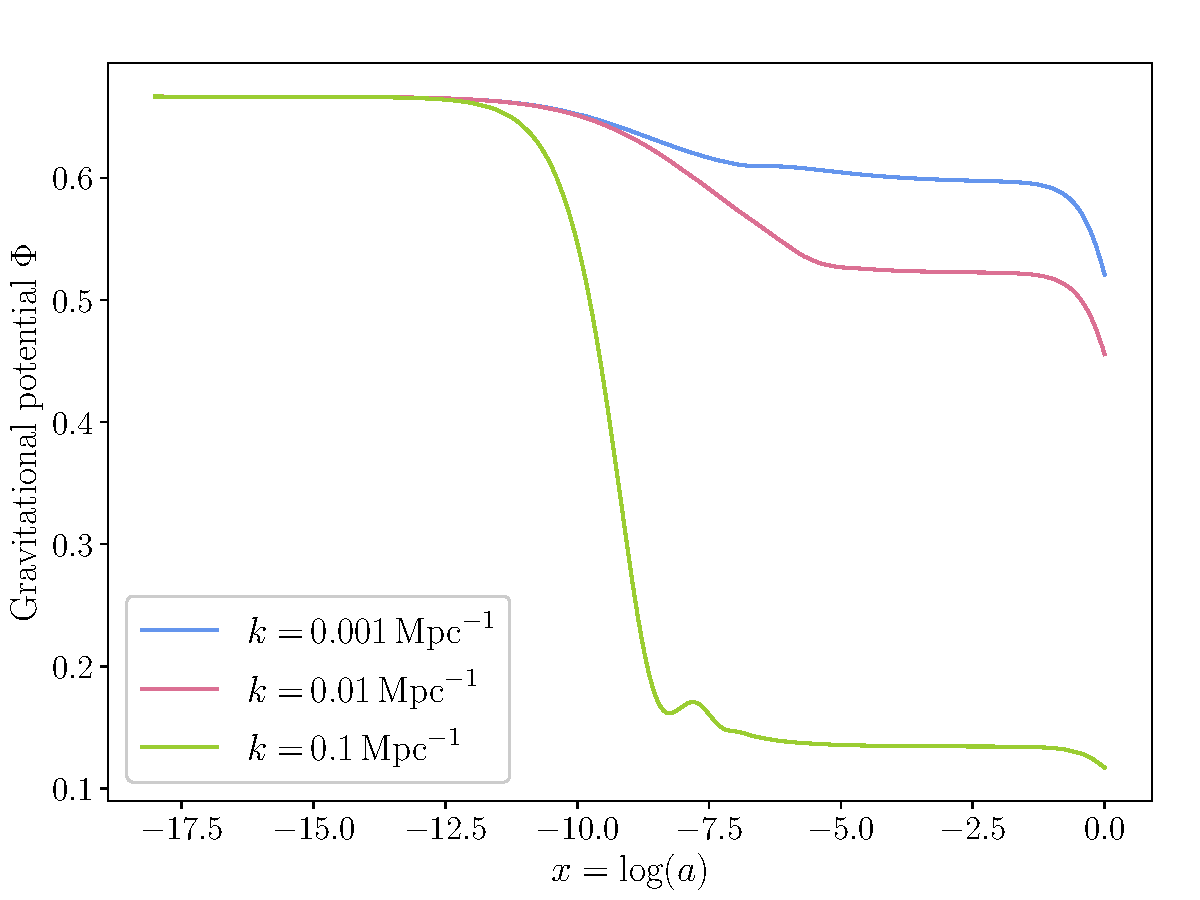
\includegraphics[width=0.98\linewidth]{/Users/paljettrosa/Documents/GitHub/AST5220/figs/toy/Phi.pdf}
    \caption{Evolution of the gravitational potential $\Phi$ on small (green), intermediate (red) and large (blue) scales in Winther's toy cosmological model. Polarization and neutrinos are not included.}\label{appfig: Phi}
  \end{minipage}
  \vspace{-20pt}
\end{figure}

% \newpage

\begin{figure}[h!]
  \centering
  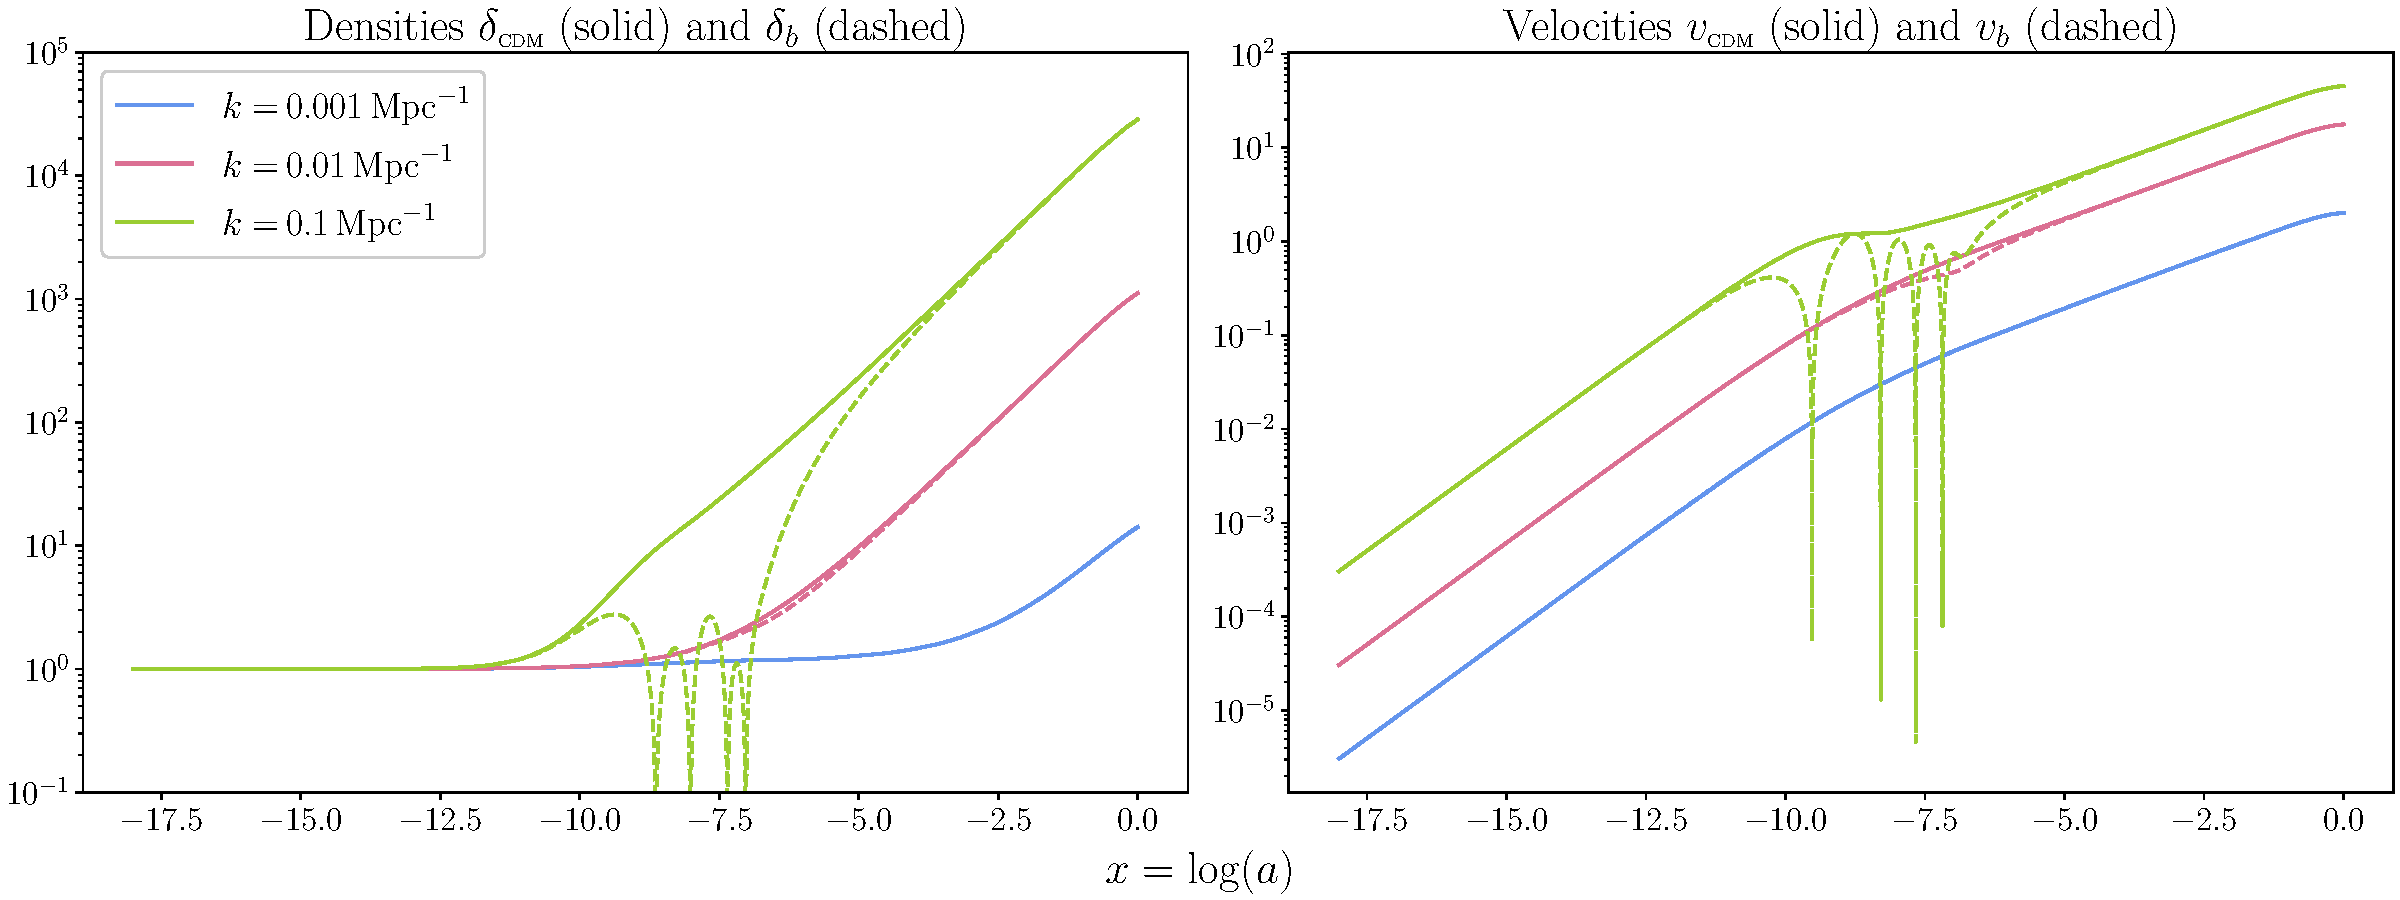
\includegraphics[width=0.95\textwidth]{/Users/paljettrosa/Documents/GitHub/AST5220/figs/toy/delta_and_v.pdf}
  \caption{Evolution of the CDM and baryon density (left) and velocity (right) perturbations on small (green), intermediate (red) and large (blue) scales in Winther's toy cosmological model. Dashed lines are used for baryons. The absolute values are plotted, since they can be negative and a logarithmic $y$-axis is used. Polarization and neutrinos are not included.}\label{appfig: delta_and_v}
\end{figure}

\begin{figure}[h!]
  \vspace{5pt}
  \centering
  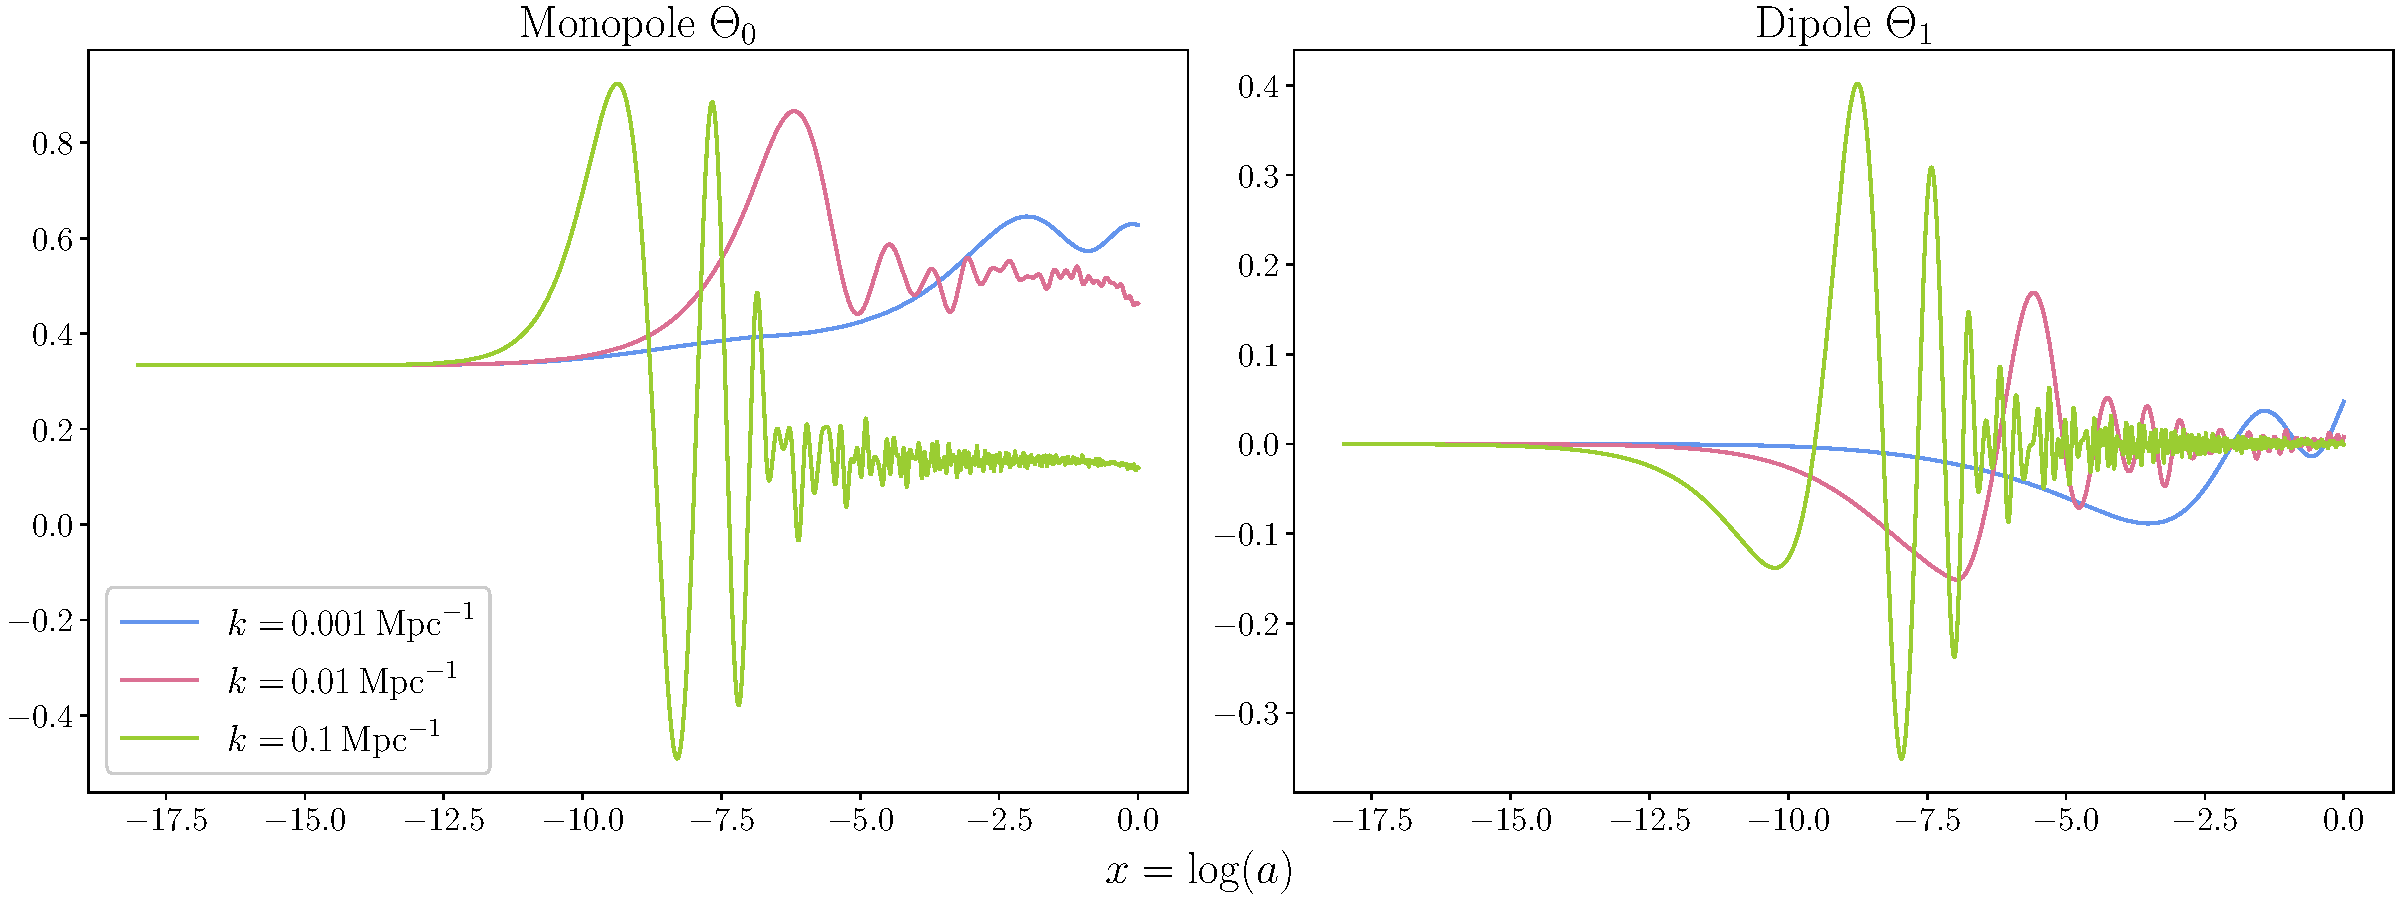
\includegraphics[width=0.95\textwidth]{/Users/paljettrosa/Documents/GitHub/AST5220/figs/toy/Thetas.pdf}
  \caption{Evolution of the photon monopole $\Theta_0$ (left) and dipole $\Theta_1$ (right) on small (green), intermediate (red) and large (blue) scales in Winther's toy cosmological model. Polarization and neutrinos are not included.}\label{appfig: Thetas}
\end{figure}


\begin{figure}[h!]
  \vspace{5pt}
  % \subsection{Milestone IV}\label{appsubsec: fig IV}
  \centering
  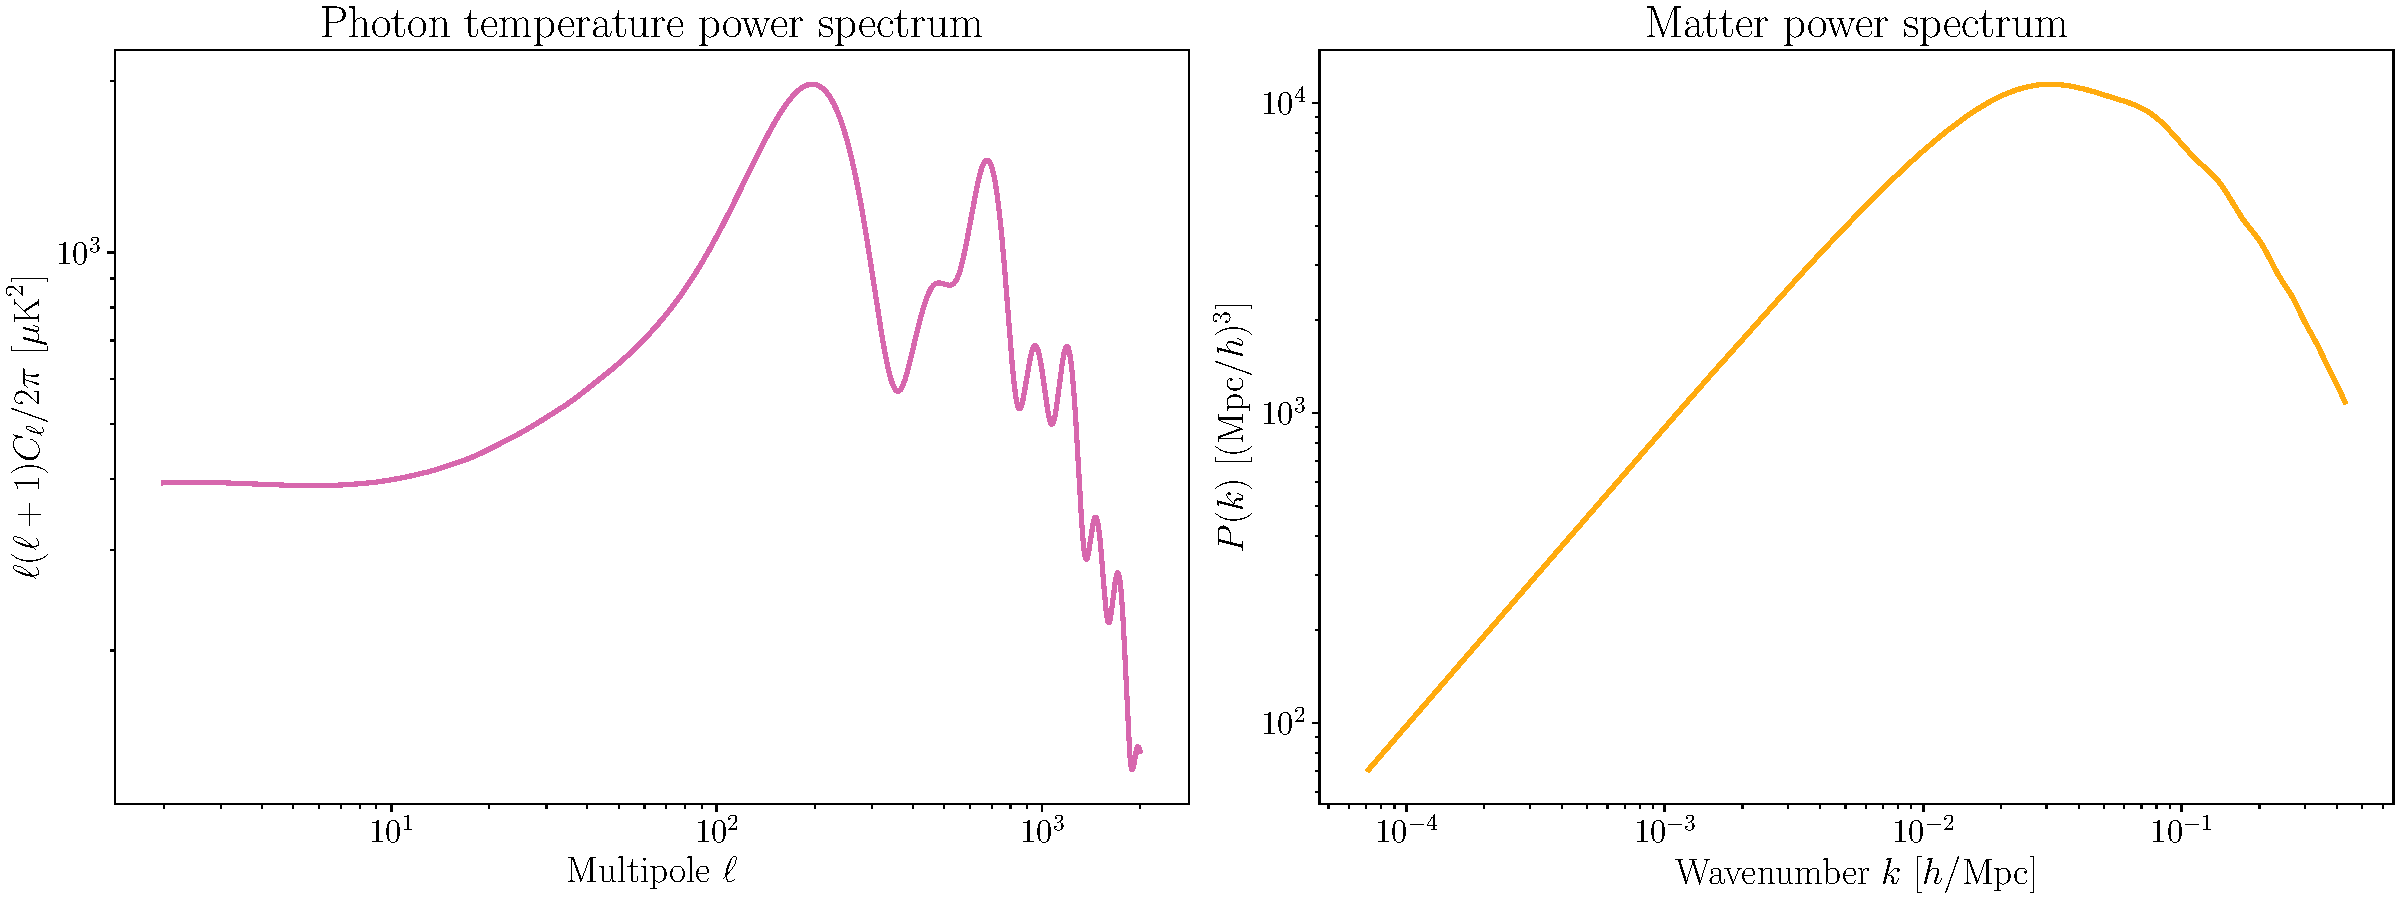
\includegraphics[width=0.95\textwidth]{/Users/paljettrosa/Documents/GitHub/AST5220/figs/toy/C_ell_and_P_k.pdf}
  \caption{The CMB power spectrum $\ell(\ell+1)C_\ell/2\pi$ (left) and matter power spectrum $P(k)$ (right) in Winther's toy cosmological model. Helium, reionization, polarization and neutrinos are not included. The parameters used for the primordial power spectrum are $A_s=10^{-9}$, $n_s=0.965$ and $k_\text{pivot}=0.05\,\text{Mpc}^{-1}$.}\label{appfig: C_ell_and_P_k}
\end{figure}

\twocolumn

\end{document}